\begin{flushright} {\tiny {\color{gray} chapter8.tex}} \end{flushright}

Solving the Stokes equations and the energy equations is one thing. Doing it in 
a geodynamical context requires a lot of additional techniques. 
\newpage %-----------------------------------------------------------------------------------------
\subsection{Dealing with a free surface (and mesh deformation)}\label{sec:freesurface} \index{general}{Free Surface}


When carrying out global models, typically  mantle convection, the effect of the free surface
is often neglected/negligeable: topography ranges from $\sim$ 10km depth to $\sim$ 10km height, which 
is very small compared to the depth of the mantle ($\sim$ 3000km). 

However, it has long been regognised that there is a feedback between topography and crust/lithosphere
deformation: the surface of the Earth reflects the deeper processes, from orogeny, back-arc basins, 
rifts, mid-ocean ridges, etc ... (see for instance \cite{brau10}).

\begin{remark}
Free surface flows are not unique to Earth sciences, and their modelling has given rise to many studies 
and textbooks. A typical free-surface flow problem in the CFD literature is the so-called 'dam break' 
problem \cite{moeb99,bacp07,liir07,lemx08,homa09,anco09}. Other occurrences involve 
sea waves, flow over structures, flow around ships, mould filling, flow with bubbles \cite{liir07}.
\end{remark}
 
What distinguishes geodynamics free surface modelling from its engineering 
counterpart is (i) the absence of surface tension, (ii) the fact that the fluids under consideration are
Stokesian, (iii) their rheology is complex (the elastic and plastic components can be 
dominant at the surface).

%There are to main modelling approaches employed in Computational Geodynamics: the so-called 
%'sticky air' approach and the Arbitrary-Lagrangian approach.

The problem of dealing with a free surface can be deceptively simple at first glance: as mentioned before the
amplitude of surface movement is often less than 1\% of the domain size. Isostacy-driven movements are
easy to deal with since the movement is vertical (and often characteried by  long wavelength). However, computational 
problems quickly arise in subduction modelling: the downgoing lithosphere subducts below the 
overriding plate and the relative convergence of the two is likely to generate a cusp at the trench. The presence
of shear bands intersecting the surface accentuates the problem:

\begin{center}
\includegraphics[width=13cm]{images/freesurface/matv15} \\
{\tiny Taken from Maffione et al \cite{matv15}. Example of free surface deformation above 
intra-oceanic subduction initiation}
\end{center}

\begin{remark} It is difficult to talk about free surface without including the underlying mesh. What follows
should be read alongside Section~\ref{sec:meshes}.
\end{remark}

%.......................................
\subsubsection{The fully Lagrangian approach}

\index{general}{Bow-tied element}

In this case the mesh is deformed with the velocity (or displacement) computed on its nodes. 
It is sometimes called 'body fitting' \cite{crsg12} or 'boundary fitted'. 
In the case when large deformation occurs (which is rather frequent in geodynamics - 
think about subduction or rifting processes where materials end up moving 100's or 1000's of km, horizontally
and/or vertically), it leads to highly deformed elements, and in some case even bow-tied:

\begin{center}
\frame{\includegraphics[width=4.5cm]{images/freesurface/b00}}
\frame{\includegraphics[width=4.5cm]{images/freesurface/b01}}
\frame{\includegraphics[width=4.5cm]{images/freesurface/b02}}\\
\frame{\includegraphics[width=4.5cm]{images/freesurface/b03}}
\frame{\includegraphics[width=4.5cm]{images/freesurface/b05}}
\frame{\includegraphics[width=4.5cm]{images/freesurface/b07}}\\
\frame{\includegraphics[width=4.5cm]{images/freesurface/b08}}
\frame{\includegraphics[width=4.5cm]{images/freesurface/b09}}
\frame{\includegraphics[width=4.5cm]{images/freesurface/b10}}\\
{\tiny Example of a free surface evolution above a sinking sphere. The isostatic rebound above the sphere 
generates a cusp which, if no special measure is taken, ultimately leads to a bow-tied element. Once this 
occurs the simulation stops since the mapping of the bow-tied element to the reference element yields to
wrong elemental matrix. Curtesy of M. Fraters}
\end{center}

In the mildest cases this does not occur but it has long been established that 
large mesh deformation yields low accuracy calculations, 
especially when angles between edges become small or large. 
One way to overcome this problem is to remesh, i.e. generate a better mesh based on the 
available information on the deformed one. In 2D this is routinely done, especially when 
triangular elements are used. In 3D, multiple remeshing are very costly and it is generally
avoided.  
Note also that re-meshing often involves some form of interpolation and therefore some unwanted 
numerical diffusion. 
When deformation is reasonably small, fully lagrangian methods work and have been used in 
geodynamics \cite{hach96b,mera80,labp00}.

\begin{center}
\includegraphics[width=8cm]{images/freesurface/labp00}\\
{\captionfont Taken from \cite{labp00}. Upper-crustal faulting, note that the bottom and the top surface are deformed.}
\end{center}


\begin{center}
\begin{minipage}{0.45\textwidth}
\centering
\includegraphics[width=7cm]{images/freesurface/guez96}\\
{\captionfont Taken from \cite{guez96}. Subduction model, topographic expression is shown without vertical exaggeration}. 
\end{minipage}\hfill
\begin{minipage}{0.45\textwidth}
\centering
\includegraphics[width=6cm]{images/freesurface/gowo93}\\
{\captionfont Taken from \cite{gowo93}. Asymmetric lithospheric extension.}
\end{minipage}
\end{center}







GET:
Crook et al. 2006, and references therein \cite{crwy06})
Beaumont et al. 1994;  \cite{befh94}


%.......................................
\subsubsection{The Eulerian approach: using sticky air}
\index{general}{Sticky Air}

Sticky air is the default option for numerical methods which mesh 
cannot be deformed (typically the finite difference method).
In this case, the air above the crust/sediments is modelled as a zero-density fluid with 
very low viscosity (see for instance the early article by Zaleski and Julien \cite{zaju92}). 
One problem quickly arises when one realises that the viscosity of the 
air ($\sim 18.5\cdot10^{-6}$ Pa$\cdot$s\footnote{\url{https://en.wikipedia.org/wiki/Viscosity}})
is almost 25-30 orders of magnitude lower than the (effective) viscosity of Earth materials. 
Real air viscosity cannot therefore be used because of 1) round-off errors, 2) extremely 
poorly-conditioned matrices. Low viscosities around $10^{16}-10^{19}$Pa$\cdot$s are then 
commonly used as they are still negligible next to those of the (plastic) crust, and the 
flow of air parallel to Earth materials only generates extremely small shear and normal stress values
(thereby approaching the true nature of a free surface). 
This approach is the one employed in all the papers based on the I2/I3(EL)VIS code (see Appendix~\ref{app:codes})
and has been benchmarked in Crameri et al. \cite{crsg12}.

This approach has a few advantages:
\begin{enumerate}
\item it is simple to implement 
\item it is compatible with all the standard numerical methods (FEM, FDM,FVM)
\item it avoids (potentially complicated) remeshing
\end{enumerate}
and quite a few drawbacks:
\begin{enumerate}
\item it increases the size of the computational domain, thereby adding more unknowns to the linear system: in \cite{scbe08} the air layer is set to 50km while the lithospheric domain underneath is 700km thick;
\item it requires the use of averaging all along the free-surface
where very large viscosity contrasts are present. Here is what Poliakov and Podlachikov \cite{popo92}
say about the sticky air method:
"Zaleski \& Julien \cite{zaju92} used a top layer with a very low
viscosity and density to represent air or water above the
surface. This allows a simple representation of the free
surface. However, due to the very high viscosity and density
contrast and diffusion between the top layer and the
underlying layers, calculations sometimes become unstable
and give significant errors."

\item it can showcase air entrainment:
\begin{center}
\includegraphics[width=8cm]{images/freesurface/scbe08}\\
{\small Taken from \cite{scbe08}. Details of the entrainment and lubrication of the soft surface layer. 
Light blue particles are sticky air particle and are found to greatly alter the viscosity
of the subduction channel.}
\end{center}
\item it is not clear how thick the air layer must be
\item it often requires to ascribe thermal parameters to the air;
\item it makes the implementation of Dirichlet or Neuman boundary conditions for temperature at the surface less
obvious.
\item it makes the coupling with surface processes codes less straightforward.
\item its accuracy depends on the method used to track materials in the rest of the code (markers, level sets, ...). If markers are used, the free surface position is then known up to the average distance between markers.
\item it negatively impacts the condition number of the matrix.
\end{enumerate}

The sticky air approach is employed by various codes in the subduction benchmark study \cite{scbe08}

The term 'sticky water' is sometimes employed too. The dynamic viscosity of water is about 
$10^{-3}$Pa$\cdot$s so that it is also negligible compared to the viscosity of Earth materials
and the same reasonng as air applies. However, in such a case a density of about 1000kg/m$^3$ 
is then assigned to the layer. REF?

In conclusion, as stated in \cite{crsg12}: "the sticky air method is a good way to
simulate a free surface for Eulerian approaches, provided that its
parameters are chosen carefully."


%..........................................................
\subsubsection{The Arbitrary Lagrangian Eulerian (ALE) approach}
\index{general}{Arbitrary Lagrangian Eulerian} \index{general}{ALE}

It is a very widely used approach in FEM-based geodynamics codes but originates in the field of 
CFD \cite{hiac74,hulz81} and is described at length in \cite{sozo01,dohp04,dohu03}.
To put it very simply, the key idea in the ALE formulation is
the introduction of a computational mesh which can move and deform with a velocity 
independent of the velocity carried by the material particles.

\paragraph{The simple approach in \cite{thie11}.}
What follows is written with a 2D Cartesian model in mind ($Q_1\times P_0$ elements are used).
The computational domain is a rectangle of size $L_x \times  L_y$ 
and a nnx $\times$ nny rectangular grid spanning the simulation
domain is generated.
The grid points constituting the top row of the grid define the
discrete free surface of the domain. Once the Eulerian velocity field
has been computed on these, their position is first updated using a
simple Eulerian advection step (see a,b on figure hereunder):
\[
\vec{r}_i'(t+\delta t) = \vec{r}_i(t) + \vec{v}_i \cdot \delta t
\qquad\qquad
i=1,\dots nnx
\]
The other boundaries of the system remain fixed at locations
$x=0$, $x=L_x$ and $y=0$. Even though the Eulerian grid must conform
to the current domain shape, only vertical motion of grid nodes is
allowed. It is therefore necessary to resample the predicted free
surface given by $\vec{r}_i'$ at equidistant positions between $x=0$ and $x=L_x$.
The resampling is carried out either with Spline functions or a 
moving least square algorithm. 
Finally, the vertical position of all the nodes corresponding
to column $i\in [1,nnx]$ is recalculated so that they are equidistant, 
as sketched in Figure d. This has the advantage of keeping
the mesh distortion to a minimum in the case of large
deformation.

\begin{center}
\includegraphics[width=9cm]{images/freesurface/ale2d}\\
 {\small The ALE algorithm of \cite{thie11} in 2D. 
(a) Grid and free surface at a given time $t$; 
(b) advection of the free surface; 
(c) resampling of the free surface at equidistant abscissae; 
(d) vertical adjustment of grid nodes in each column at equidistant ordinates.}
\end{center}

The ALE method is used in the SOPALE, SULEC, FANTOM, ELEFANT, and ASPECT codes to name a few
(see Appendix~\ref{app:codes}).


\paragraph{The not-so-simple but rather elegant approach of ASPECT}

What follows is mostly borrowed from Rose et al \cite{robh17}. Their approach 
has the advantage that it does not presuppose a geometry (Cartesian, Spherical, ...)
nor a number of dimensions. It is also designed to work in parallel and on octree-based
meshes, and with various combinations of boundary conditions.
Note that the authors specify that "for moderate mesh deformation, the mesh stays smooth and well
conditioned, though it breaks down for large deformations".


This approach is obtained by simply imposing the obvious condition 
that no particle (fluid parcel) can cross the free surface (because it is a material surface). 
This can be imposed in a straightforward manner by using a Lagrangian description along this surface. 
However, this condition may be relaxed by imposing only the necessary 
condition: $\vec{\upnu}$ equal to zero along the normal to the boundary 
(ie. $\vec{n}\cdot\vec{\upnu} = 0$, where $\vec{n}$ is the outward unit 
normal to the fluid domain). 
The mesh position, normal to the free surface, is determined from the normal component of 
the particle velocity 
and remeshing can be performed along the tangent; 
see, for instance Huerta and Liu, 1989 \cite{huli88} or Braess and Wriggers, 2000 \cite{brwr00} 

As mentioned above the mesh velocity in normal direction at the free surface (with
unit normal $\vec{n}$) has to be consistent with the velocity of the Stokes
velocity solution $\vec{\upnu}(t)$:
\begin{equation}
\vec{\upnu}_{\text{mesh}}(t)\cdot \vec{n} = \vec{\upnu}(t)\cdot \vec{n} 
\qquad
\text{on}
\quad
\Gamma_F
\end{equation}
In ALE calculations the internal mesh velocity is usually undetermined, 
but one wants to smoothly deform the mesh so as to preserve its regularity, 
avoiding inverted or otherwise poorly conditioned cells. 
The mesh deformation can be calculated in many different ways, icluding algebraic 
(as mentioned in the previous paragraph) and PDE based approaches.
The latter is chosen here. 
The Laplace equation is solved where the unknown is the mesh velocity, i.e. 
one must solve:
\begin{equation}
\Delta \vec{\upnu}_{\text{mesh}} = 0\label{eq:fsaspect1}
\end{equation}
subjected to the following boundary conditions:
\begin{eqnarray}
\vec{\upnu}_{\text{mesh}} &=& \vec{0} \qquad\qquad \text{on } \Gamma_0 \\
\vec{\upnu}_{\text{mesh}} &=& (\vec{\upnu}\cdot\vec{n})\vec{n} \qquad \text{on } \Gamma_F \\
\vec{\upnu}_{\text{mesh}}\cdot \vec{n} &=& 0 \qquad\qquad \text{on } \Gamma_{FS} \label{eq:fsaspect2}
\end{eqnarray}
where $\Gamma_{FS}$ is the part of the boundary with free slip boundary conditions, 
$\Gamma_0$ is the no-slip part and $\Gamma_{FS}$ is the free slip part.

Once the mesh velocity has been obtained for all mesh points, these can be moved with 
said velocity. However, it must be noted that the multiple occurences of the normal vector
in the above equations is not without problem as the normal vectors are not well defined on the
mesh vertices, which is where the mesh velocity is defined.

This yields what the author coin the 'quasi-implicit' scheme 
(we have so far neglected any kind of stabilisation):
\begin{enumerate}
\item Solve the Stokes system;
\item Solve for the surface mesh velocity using Equation~\ref{eq:fsaspect3};
\item Solve for the internal mesh velocity using Equations~\ref{eq:fsaspect1}, \ref{eq:fsaspect2}; 
\item Advect the mesh forward in time using displacements determined by
the forward Euler scheme: $\vec{x}(t^{n+1} ) = \vec{x}(t^n ) + \vec{\upnu}_{\text{mesh}} \delta t$.
\end{enumerate}

Note that Rose et al (2017) \cite{robh17} go further than this, propose a 'nonstandard finite difference scheme' 
and make a link with the stabilisation presented in Kaus et al (2010) \cite{kamm10}.

The authors list two simple methods of computing the normals:
\begin{itemize}
\item one can take $\vec{n}$ as the direction of the local vertical,
\item one could compute $\vec{n}$ as some weighted average of the cell normals adjacent to a given
vertex
\end{itemize}
but conclude that they have found that these schemes do not necessarily
have good mass conservation properties.

A better approach is proposed in the form of an $L_2$ projection of the 
normal velocity $\vec{v}\cdot\vec{n}$ onto the free surface $\Gamma_F$. 
Multiplying the boundary conditions 
\[
\vec{\upnu}_{\text{mesh}} = (\vec{\upnu}\cdot\vec{n})\vec{n} 
\]
by a test function $\vec{w}$ and integrating over the free surface part of the boundary, we find:
\begin{equation}
\int_{\Gamma_F} \vec{w}\cdot\vec{\upnu}_{\text{mesh}} d\Gamma 
=
\int_{\Gamma_F} \vec{w}\cdot (\vec{\upnu}\cdot\vec{n})\vec{n} d\Gamma
=
\int_{\Gamma_F} (\vec{w}\cdot\vec{n}) (\vec{\upnu}\cdot\vec{n}) d\Gamma \label{eq:fsaspect3}
\end{equation}
When discretized, this forms a linear system which can be solved for the mesh velocity 
$\vec{\upnu}_{\text{mesh}}$ at the free surface. 
This system, being nonzero over only the free surface, is relatively computationally inexpensive to solve.
The authors unfortunately fail to mention that this approach is particularly 
interesting since the numerical quadrature used to compute the above integrals
require the normal $\vec{n}$ between the nodes and these normals are well defined over each 
segment joining two nodes!\footnote{what if $Q_k$ with $k>1$ elements are used and nodes on the surface
no more form a line? }

In what follows I present in some detail how to carry out the $L_2$ projection to arrive at the surface velocity
for both $Q_1$ and $Q_2$ elements.

I start from the following integral over a $Q_1$ element:
\begin{eqnarray}
\int_{\Gamma_e} N_i \vec{\upnu}_{mesh} d\Gamma
&=& \int N_i \left( \begin{array}{c} u_{mesh} \\ v_{mesh} \end{array} \right) d\Gamma \\
&=& \int N_i 
\left( \begin{array}{cccc}  N_1 & 0 & N_2 & 0 \\ 0 & N_1 & 0 & N_2  \end{array}\right)\cdot
\left( \begin{array}{c} u_1 \\ v_1 \\ u_2 \\ v_2 \end{array} \right) d\Gamma \\
\end{eqnarray}
Writing this equation alternatively for $N_i=N_1,N_2$ yields:
\[
\int_{\Gamma_e} 
\left( \begin{array}{cccc}  
N_1N_1 & 0 & N_1N_2 & 0 \\ 
0 & N_1N_1 & 0 & N_1N_2 \\
N_2N_1 & 0 & N_2N_2 & 0 \\ 
0 & N_2N_1 & 0 & N_2N_2 
\end{array}\right)
\cdot \left( \begin{array}{c} u_1 \\ v_1 \\ u_2 \\ v_2 \end{array} \right) 
d\Gamma 
=
\int_{\Gamma_e} 
\left( \begin{array}{cccc}  
N_1N_1 & 0 & N_1N_2 & 0 \\ 
0 & N_1N_1 & 0 & N_1N_2 \\
N_2N_1 & 0 & N_2N_2 & 0 \\ 
0 & N_2N_1 & 0 & N_2N_2 
\end{array}\right)
d\Gamma \quad 
\cdot \left( \begin{array}{c} u_1 \\ v_1 \\ u_2 \\ v_2 \end{array} \right) 
\]
Turning now to the right hand side %(I denote by $\vec{n}_e$ the normal to the element edge):
$\int_{\Gamma_e} N_i   (\vec{\upnu}\cdot\vec{n}_e)\vec{n}_e  d\Gamma$, it yields the following rhs:
\[
\int_{\Gamma_e}   (\vec{\upnu}\cdot\vec{n}_e)
\left(\begin{array}{c}
N_1 n_x \\ N_1 n_y \\ N_2 n_x \\ N_2 n_y
\end{array}\right)
 d\Gamma
\]
The elemental matrix and rhs must be built for each element and assembled in a 
global matrix and rhs. The solution is the mesh velocity vector at all surface nodes.
the same approach can be taken for $Q_2$ elements:
\begin{eqnarray}
\int_{\Gamma_e} N_i \vec{\upnu}_{mesh} d\Gamma
&=& \int N_i \left( \begin{array}{c} u_{mesh} \\ v_{mesh} \end{array} \right) d\Gamma \\
&=& \int N_i 
\left( \begin{array}{cccccc}  
N_1 & 0 & N_2 & 0 & N_3 & 0\\ 
0 & N_1 & 0 & N_2 & 0 & N_3 
\end{array}\right)\cdot
\left( \begin{array}{c} u_1 \\ v_1 \\ u_2 \\ v_2 \\ u_3 \\ v_3 \end{array} \right) d\Gamma 
\end{eqnarray}
Writing this equation alternatively for $N_i=N_1,N_2,N_3$ yields:
\begin{eqnarray}
&&\int_{\Gamma_e} 
\left( \begin{array}{cccccc}  
N_1N_1 & 0 & N_1N_2 & 0 & N_1N_3 & 0 \\ 
0 & N_1N_1 & 0 & N_1N_2 & 0 & N_1N_3 \\
N_2N_1 & 0 & N_2N_2 & 0 & N_2N_3 & 0 \\ 
0 & N_2N_1 & 0 & N_2N_2 & 0 & N_2N_3 \\
N_3N_1 & 0 & N_3N_2 & 0 & N_3N_3 & 0 \\ 
0 & N_3N_1 & 0 & N_3N_2 & 0 & N_3N_3 \\
\end{array}\right)
\cdot \left( \begin{array}{c} u_1 \\ v_1 \\ u_2 \\ v_2 \\ u_3 \\ v_3 \end{array} \right) 
d\Gamma \nn\\ 
&=&
\int_{\Gamma_e} 
\left( \begin{array}{cccccc}  
N_1N_1 & 0 & N_1N_2 & 0 & N_1N_3 & 0 \\ 
0 & N_1N_1 & 0 & N_1N_2 & 0 & N_1N_3 \\
N_2N_1 & 0 & N_2N_2 & 0 & N_2N_3 & 0 \\ 
0 & N_2N_1 & 0 & N_2N_2 & 0 & N_2N_3 \\
N_3N_1 & 0 & N_3N_2 & 0 & N_3N_3 & 0 \\ 
0 & N_3N_1 & 0 & N_3N_2 & 0 & N_3N_3 
\end{array}\right)
d\Gamma \quad 
\cdot \left( \begin{array}{c} u_1 \\ v_1 \\ u_2 \\ v_2 \\ u_3 \\ v_3 \end{array} \right) 
\end{eqnarray}

The right hand side is then  
\[
\int_{\Gamma_e}   (\vec{\upnu}\cdot\vec{n}_e)
\left(\begin{array}{c}
N_1 n_x \\ N_1 n_y \\ 
N_2 n_x \\ N_2 n_y \\
N_3 n_x \\ N_3 n_y 
\end{array}\right)
 d\Gamma
\]
Having obtained the boundary condition velocity for the Laplace equation, we can now turn our attention 
to solving this ODE. 


Note that Rose et al (2017) \cite{robh17} go further than this and propose a 'nonstandard finite difference scheme' and make a link with the stabilisation presented in Kaus et al (2010) \cite{kamm10}.

In what follows I omit the subscript 'mesh' and focus on the 2D case. The components of the (mesh) velocity
are given by
\[
u^h = \sum_{i=1}^{m_\upnu} N_i^\upnu u_i
\qquad
\qquad
v^h = \sum_{i=1}^{m_\upnu} N_i^\upnu v_i
\qquad
\qquad
\vec{\upnu}^h=\left( 
\begin{array}{c}
u^h \\
v^h 
\end{array}  \right)
\]
We start from the ODE to solve in its strong form:
\[
\Delta \vec{\upnu}^h = \vec{0}
\]
We multiply it by a velocity test function $N_i^\upnu$ and integrate over an element: 
\begin{eqnarray}
&&\vec 0 \nonumber\\
&=& \int_{\Omega_e} N_i^\upnu  \Delta \vec{\upnu}^h \nonumber\\ 
&=&\int_{\Omega_e} N_i^\upnu \Delta \vec\upnu^h dV \nonumber\\
&=&\int_{\Omega_e}  \left(\begin{array}{c}
N_i^\upnu \Delta u^h \\
N_i^\upnu \Delta v^h 
\end{array}\right) dV \nonumber\\
&=&\int_{\Omega_e}  \left(\begin{array}{c}
N_i^\upnu \vec\nabla \cdot \vec\nabla u^h \\
N_i^\upnu \vec\nabla \cdot \vec\nabla v^h 
\end{array}\right) dV \nonumber\\
&=&
\int_{\Omega_e}   \left(\begin{array}{c}
\vec\nabla N_i^\upnu \cdot \vec\nabla u^h \\
\vec\nabla N_i^\upnu \cdot \vec\nabla v^h 
\end{array}\right) dV \nonumber\\
&=&
\int_{\Omega_e}
\left(\begin{array}{c}
\partial_x N_i^\upnu \partial_x u^h + \partial_y N_i^\upnu \partial_y u^h \\ 
\partial_x N_i^\upnu \partial_x v^h + \partial_y N_i^\upnu \partial_y v^h 
\end{array}\right) dV \nonumber\\
&=&\int_{\Omega_e}
\left(
\begin{array}{cccc}
\partial_x N_i^\upnu & \partial_y N_i^\upnu & 0 & 0 \\ 
0 & 0 & \partial_x N_i^\upnu & \partial_y N_i^\upnu  \\ 
\end{array}
\right)
\!\cdot\!
\left(
\begin{array}{c}
\partial_x u^h \\
\partial_y u^h \\
\partial_x v^h \\
\partial_y v^h 
\end{array}
\right) dV \nonumber\\
&=&\int_{\Omega_e}
\left(
\begin{array}{cccc}
\frac{\partial N_i^\upnu}{\partial x} & \frac{\partial N_i^\upnu}{\partial y} & 0 & 0 \\ 
0 & 0 & \frac{\partial N_i^\upnu}{\partial x} & \frac{\partial N_i^\upnu}{\partial y}  \\ 
\end{array}
\right)
\!\cdot\!
\left(
\begin{array}{cccccccccc}
\frac{\partial N_1^\upnu}{\partial x} & 0  & \frac{\partial N_2^\upnu}{\partial x} & 0  & \cdots & \frac{\partial N^\upnu_{m_\upnu}}{\partial x} & 0 \\ \\
\frac{\partial N_1^\upnu}{\partial y} & 0  & \frac{\partial N_2^\upnu}{\partial y} & 0  & \cdots & \frac{\partial N^\upnu_{m_\upnu}}{\partial y} & 0 \\ \\
0 & \frac{\partial N_1^\upnu}{\partial x}  & 0& \frac{\partial N_2^\upnu}{\partial x}  & \cdots & 0 & \frac{\partial N^\upnu_{m_\upnu}}{\partial x}  \\ \\
0 & \frac{\partial N_1^\upnu}{\partial y}  & 0& \frac{\partial N_2^\upnu}{\partial y}  & \cdots & 0 & \frac{\partial N^\upnu_{m_\upnu}}{\partial y}  
\end{array}
\right) 
\!\cdot\!
\left(
\begin{array}{c}
u_1 \\ v_1 \\ u_2 \\ v_2 \\ \dots \\ u_{m_v} \\ v_{m_v} 
\end{array}
\right) dV \nonumber
\end{eqnarray}
Writing this equation for $i=1,...m_\upnu$, we obtain:
\[
\int
\left(
\begin{array}{cccc}
\frac{\partial N_1^\upnu}{\partial x} & \frac{\partial N_1^\upnu}{\partial y} & 0 & 0 \\ 
0 & 0 & \frac{\partial N_1^\upnu}{\partial x} & \frac{\partial N_1^\upnu}{\partial y}  \\ 
\frac{\partial N_2^\upnu}{\partial x} & \frac{\partial N_2^\upnu}{\partial y} & 0 & 0 \\ 
0 & 0 & \frac{\partial N_2^\upnu}{\partial x} & \frac{\partial N_2^\upnu}{\partial y}  \\ 
\vdots & \vdots & \vdots & \vdots \\
\vdots & \vdots & \vdots & \vdots \\
\frac{\partial N_{m_\upnu}^\upnu}{\partial x} & \frac{\partial N_{m_\upnu}^\upnu}{\partial y } & 0 & 0 \\ 
0 & 0 & \frac{\partial N_{m_\upnu}^\upnu}{\partial x} & \frac{\partial N_{m_\upnu}^\upnu}{\partial y}  \\ 
\end{array}
\right)
\cdot
\left(
\begin{array}{cccccccccc}
\frac{\partial N_1^\upnu}{\partial x} & 0  & \frac{\partial N_2^\upnu}{\partial x} & 0  & \cdots & \frac{\partial N^\upnu_{m_\upnu}}{\partial x} & 0 \\ \\
\frac{\partial N_1^\upnu}{\partial y} & 0  & \frac{\partial N_2^\upnu}{\partial y} & 0  & \cdots & \frac{\partial N^\upnu_{m_\upnu}}{\partial y} & 0 \\ \\
0 & \frac{\partial N_1^\upnu}{\partial x}  & 0& \frac{\partial N_2^\upnu}{\partial x}  & \cdots & 0 & \frac{\partial N^\upnu_{m_\upnu}}{\partial x}  \\ \\
0 & \frac{\partial N_1^\upnu}{\partial y}  & 0& \frac{\partial N_2^\upnu}{\partial y}  & \cdots & 0 & \frac{\partial N^\upnu_{m_\upnu}}{\partial y}  
\end{array}
\right) 
\cdot
\underbrace{
\left(
\begin{array}{c}
u_1 \\ v_1 \\ u_2 \\ v_2 \\ \dots \\ u_{m_v} \\ v_{m_v} 
\end{array}
\right) }_{\vec V}
dV
=\vec{0}
\]
or, 
\[
\left( \int_{\Omega_e} {\bm B}^T  \cdot {\bm B} \; dV \right)\cdot \vec{V} = \vec{0}
\]
where ${\bm B}$ is a $(ndim*ndim) \times (m_v*ndofV)$ matrix. This is implemented in Stone 54 \ref{f54}.

\begin{remark}
The integration by parts should have a minus appear but since the left hand side 
is 0, it is not taken into account. 
\end{remark}

\todo[inline]{surface terms arising from the integration by parts are neglected. EXPLAIN WHY!}


\paragraph{Yet another approach \cite{dohp04}}
The unknown position of free surfaces can be computed using the following approach:
for the simple case of a single-valued function $h=h(x,y,t)$, a hyperbolic equation must be solved,
\begin{equation}
\frac{\partial h}{\partial t} + (\vec{ \upnu}\cdot \vec{ \nabla}) h = 0    \label{eqfs1}
\end{equation}
This is the kinematic equation of the surface and has been used, for instance, 
by Ramaswamy and Kawahara (1987), Huerta and Liu, 1988b, 1990; Souli and Zolesio (2001).





\underline{Idea:} Eq. (\ref{eqfs1}) is a simple advection equation. 
One could also add a diffusion operator with a diffusion coefficient $D$.
Low values of $D$ could be used to stabilise the surface while 
higher values (possibly nonlinear ones) could be used to account for simple 
surface processes. 

\begin{equation}
\frac{\partial h}{\partial t} + (\vec{\upnu}\cdot\vec{ \nabla}) h = D \Delta h  \label{eqfs2}
\end{equation}

Also, Hansen and Nielsen \cite{hanl00,hani03} write:
During the entire model evolution surface processes act to re-distribute sediments. 
These processes are modelled by a diffusion equation with a source term enabling the transport 
of sediments to and from the model profile. The transport equation is written
\[
\dot{h}=\nabla\cdot (\kappa \nabla h) + \dot{s}(w)
\]
where $\kappa=200 km^2/Ma$ is the diffusivity of topography and $\dot{s}(w)$ 
is a linear function of water depth. 



The following pictures are taken from Naliboff et al \cite{nabp17} on the topic 
of how complex fault interaction controls continental rifting. It is a beautiful
example (among many) of the importance of free surface geodynamical expression
and large deformation:

\begin{center}
\includegraphics[width=9cm]{images/freesurface/nabp17a}\\
\includegraphics[width=9cm]{images/freesurface/nabp17b}\\
\includegraphics[width=14cm]{images/freesurface/nabp17c}\\
{\captionfont Taken from \cite{nabp17}}
\end{center}

%-------------------------------------------------------
\subsubsection{On the topic of moving internal nodes}

Braess \& Wriggers \cite{brwr00} propose the following interesting algorithm:
"A measure of the quality of a triangular mesh is the quotient of the
outer radius $r_{out}$ and the inner radius $r_{in}$ 
of each element. This quotient is important because it plays a
certain role in a priori error estimates. If an element degenerates this quotient will approach infinity.
Another important feature of good mesh is that no element becomes very large. With these considerations
in mind the penalty function $W$ is defined:
\begin{equation}
W = \sum_{elts} \left( \frac{r_{out}}{r_{in}} \right)^m \left( \frac{r_{out}}{r_0} \right)^n
\end{equation}
where $m$, $n$ and $r_0$ are positive constants. 
For our calculations we chose $m=3$, $n=1$ and $r_0=1$, but the results seem
to depend only slightly on this choice. Whenever a triangle is distorted or very large, this function becomes
very large. A similar penalty function was presented in \cite{jole97} for 
four-node elements. In that case the angles
of the elements are used to construct the penalty function.
In order to regularize a distorted mesh the coordinates of the internal nodes will be chosen such that $W$ is
minimized. It is not necessary to reach the global minimum, a rough approximation is sufficient.
Therefore the minimization of the potential can be done efficiently with standard procedures and will not be
discussed in any detail. This algorithm can also be applied to $h$-adaptive mesh-generation by choosing
appropriate constants $r_0$ for each triangle."\footnote{Indeed, if $r_0$ is the same for all elements
this parameter will not play any role at all in the minimisation process.} 



\vspace{4cm}
This is still WORK IN PROGRESS. I Need to look at those papers:
\cite{raka87}
\cite{huli88}\cite{pobe98}
\cite{bens89}
\cite{sucy00}
\cite{rama90}
\cite{tebm92}(moving pulse)
\cite{dumg11}
\cite{dumy16} 
\cite{anmp15}
\cite{krwd12}
\cite{stcl10}
\cite{maie12}
\cite{guez96}\cite{zhgm96}
\cite{elsp04}
\cite{brwr00}
\cite{pada83}
and talk about free surface stabilisation \cite{kamm10,qube11,dumg11,robh17}.



 
\newpage %-----------------------------------------------------------------------------------------
\subsection{Convergence criterion for nonlinear iterations\label{sec:nlconvcrit}}\begin{flushright} {\tiny {\color{gray} nlconvcrit.tex}} \end{flushright}

Disclaimer: the topic of nonlinear PDEs solving is vast and has received 
much attention from the mathematical community. In what follows I present 
a few key ideas which are at the core of many codes and publications in 
computational geodynamics.

Looking at the conservation equations that we must solve, i.e. 
conservation of mass, momentum and energy, we find that more often 
than not the coefficients of these PDEs depend on the strain rate, 
temperature, pressure, etc ... 
This makes solving the PDEs even harder. 
Also the advection term $\vec{\upnu}\cdot \vec\nabla$ couples the two primary 
variables velocity and temperature. 

One simple approach consists first in 'separating' the mass+momentum equations 
from the energy equation: one solves the first two equations assuming temperature known
while the energy equation is solved assuming velocity and pressure known. 
Better schemes obviously exist and iterate on these equations until convergence 
for velocity, pressure and temperature is reached (see for instance the \aspect manual). 
In what follows I focus on the mass and momentum equations assuming temperature known. 

The main source of nonlinearity lies in the (effective) viscosity which often
depends on strain rate and pressure (note that density can also depend on pressure
in compressible cases):
\begin{eqnarray}
\vec\nabla\cdot (2 \eta_{\rm eff}(\dot{\bm\varepsilon},p) \;  \dot{\bm\varepsilon}) 
- \vec\nabla p + \rho \vec{g} &=& \vec{0} \nn\\
\vec\nabla \cdot \vec\upnu &=& 0\nn
\end{eqnarray}
Simply put, in order to solve these equations and obtain 
the velocity and pressure fields I need to specify the density and viscosity (and of course 
appropriate boundary conditions!), but in order to compute the viscosity I need the strain rate 
and pressure fields.  

The simplest approach here consists in so-called Picard iterations as 
explained in Section~\ref{ss:picard}.

Let us start with the penalty-based FEM codes. In this case the mass and momentum 
equations are 'merged' into a single PDE where pressure has been eliminated:
\[
\vec\nabla\cdot (2 \eta_{\rm eff}(\dot{\bm\varepsilon},p) \;  \dot{\bm\varepsilon}) 
+\lambda \vec\nabla (\vec\nabla \cdot \vec\upnu) + \rho \vec{g} = \vec{0} 
\]
In this case the algorithm is simple:
\begin{enumerate}
\item start with a guess for the velocity and pressure fields, i.e. $\vec{\cal V}^{old}$ 
and $\vec{\cal P}^{old}$
\item compute the effective viscosity field with $\vec{\cal V}^{old}$ and $\vec{\cal P}^{old}$
\item solve PDE, obtain new solution $\vec{\cal V}^{new}$ 
\item compute $\vec{\cal P}^{new}$ from $\vec{\cal V}^{new}$
\item assess convergence, i.e. answer 'how close are the newly obtained fields from the old ones?'
\item $\vec{\cal V}^{old} \leftarrow \vec{\cal V}^{new}$, and $\vec{\cal P}^{old} \leftarrow \vec{\cal P}^{new}$
\item if not converged go back to 2, else exit
\end{enumerate}

Thieulot (2011) \cite{thie11} computes the means
$\langle \vec{\cal V}^i\rangle$, 
$\langle \vec{\cal V}^{i+1}\rangle$, 
and the variances 
$\sigma_{\cal V}^i$ and 
$\sigma_{\cal V}^{i+1}$ 
followed by the correlation 
\[
R^{i,i+1} = \frac{\langle (\vec{\cal V}^i - \langle \vec{\cal V}^i\rangle)
\cdot ( \vec{\cal V}^{i+1} - \langle \vec{\cal V}^{i+1}\rangle) \rangle }
{\sqrt{\sigma_{\cal V}^i \sigma_{\cal V}^{i+1}}}
\]
Since the correlation is normalised, it takes values between 0
(very dissimilar velocity fields) and 1 (very similar fields). The
following convergence criterion, formulated in terms of the variable $\chi = 1 -R^{i,i+1} $
has been implemented: convergence is reached when $\chi<tol$.
Since pressure is a derived quantity from velocity, if velocity is converged so is 
pressure\footnote{Two caveats here: the amplitude of the chequerboard mode
might come into play - in the case $Q_1\times P_0$ elements are used- and so does the applied smoothing.}.

When the algorithm above is close to convergence then $\vec{\cal V}^i$ and $\vec{\cal V}^{i-1}$ are close. 
If these were scalar quantities we could subtract them and look at the (absolute) difference: 
if it is 'small enough' then the algorithm has converged. 
However there are two problems with this: 
\begin{enumerate}
\item $\vec{\cal V}^i$ and $\vec{\cal V}^{i-1}$ are vector 
quantities (with potentially millions of values) so in order to measure a scalar difference 
between these we must take the norm of the difference, or $||\vec{\cal V}^i-\vec{\cal V}^{i-1}||$
and it is common to take the $L^2$-norm. 
\item we do not know a priori the (magnitude of the) solution so that 'small enough' is a dangerous 
statement. We could check for $||\vec{\cal V}^i-\vec{\cal V}^{i-1}||<tol$ and set $tol=10^{-6}$
for example. However in geodynamics velocities are of the order of a \si{\cm\per\year} which is 
about $3.1\cdot10^{-10}\si{\metre\per\second}$. Small velocity changes would then be enforced
only if $tol<10^{-12}$. This value might prove completely unpractical for other applications. 
In light of all this one then resorts to assessing the {\it relative} change in the velocity by normalising 
the previous quantity by the average velocity in the domain $||\vec{\cal V}^i||$.
\end{enumerate}

This is the very approach taken by Spiegelman \etal \cite{spmw16} who monitor the 
relative changes in the solution from iteration to iteration: 
\[
\frac{||\Delta \vec{\cal V} ||_{L2}}{||\vec{\cal V}||_{L2}} 
=
\left( \frac{\int\limits_\Omega (\vec{\cal V}_i-\vec{\cal V}_{i-1}) \cdot( \vec{\cal V}_i-\vec{\cal V}_{i-1}) dV}{\int\limits_\Omega \vec{\cal V}_i\cdot\vec{\cal V}_i dV} \right)^{1/2}
\]
Of course, if a mixed formulation is used where velocity and pressure are solved for unknowns,
the same monitoring can be done for pressure:
\[
\frac{||\Delta \vec{\cal P} ||_{L2}}{||\vec{\cal P}||_{L2}} 
=
\left( \frac{\int\limits_\Omega (\vec{\cal P}_i-\vec{\cal P}_{i-1}) \cdot( \vec{\cal P}_i-\vec{\cal P}_{i-1}) dV}{\int\limits_\Omega \vec{\cal P}_i\cdot\vec{\cal P}_i dV} \right)^{1/2}
\]
Convergence is reached when both are below 0.001 (as in Lemiale \etal (2008) \cite{lemm08}) 
or 0.0001 (as in Kaus \etal (2010) \cite{kaus10}).

The last option is via the nonlinear residual. Coming back to the penalty formulation, 
we can form the nonlinear residual as follows:
\[
\vec{\cal R}^i = \K(\eta_{\rm eff}(\dot{\bm\varepsilon}^{i},p^{i})) \cdot \vec{\cal V}^i - \vec{f}
\]
where $\K$ is defined in Section~\ref{sec_penalty}. 
Close to convergence $\vec{\cal V}^i$ and $\vec{\cal V}^{i-1}$
are very close so that we expect the residual $\vec{\cal R}$ to become smaller and smaller.
In order to extract a scalar from $\vec{\cal R}$ we once again resort to the $L^2$-norm and 
we also wish to to monitor its relative change. In this case it is customary to use $\vec{\cal R}^0=\vec{f}$ so 
that the convergence criterion becomes
\[
\frac{||\vec{\cal R}^i ||}{||\vec{\cal R}^0 ||} < tol.
\]

FINISH: explain problem with mixed formulation!


\begin{center}
\includegraphics[width=6cm]{images/nlconv/spmw16}\\
{\captionfont Taken from Spiegelman, May \& Wilson \etal (2016). Example of 
reported nonlinear convergence.}
\end{center}





 
\newpage %-----------------------------------------------------------------------------------------
\subsection{Strain weakening} \label{sec:strainweakening} \begin{flushright} {\tiny {\color{gray} strainweakening.tex}} \end{flushright}

Several mechanisms may contribute to strain or strain
rate dependent weakening but their relative and absolute
importance is poorly constrained. Furthermore, 
weakening mechanisms are often crudely parameterised in 
geodynamical codes with simple mathematical functions 
and a limited number of parameters. 

For example, in \cite{alht11} the authors use a von Mises plasticity formulation so that the 
rheology is parameterised by the cohesion $c$, or $c=\sigma_y$ in their notations. The
yield strength $\sigma_y$ starts is constant until the strain
$\varepsilon$ reaches the threshold value $\varepsilon_1$. It then decreases linearly
from $\sigma_y$ to $\sigma_{y}^{sw}$ between $\varepsilon_1$ and $\varepsilon_2$. 
For strain values $\varepsilon>\varepsilon_2$ , the yield strength remains constant 
at $\sigma_y^{sw}$ .

\begin{center}
\includegraphics[width=6cm]{images/strainweakening/alht11}\\
{\tiny Taken from \cite{alht11}}
\end{center}

The same authors in a subsequent study use a Drucker-Prager rheology parameterised by 
cohesion $c$ and friction angle $\phi$. They use the same approach as before but now 
both parameters are subjected to strain weakening: 

\begin{center}
\includegraphics[width=6cm]{images/strainweakening/alht12}\\
{\tiny Taken from \cite{alht12}, see also \cite{thie11}}
\end{center}

They further define the factor $R=C^0/C^{sw}=\phi^0/\phi^{sw}\geq 1$ which is a proxy
for the ratio $\sigma_y/\sigma_y^{sw}$ where $\sigma_y=p \sin\phi + c \; \cos \phi$, 
and carry out 3D crustal extensional models for $R$ between 2 and 5. 


\begin{itemize}
\item In \cite{lemh17} the authors also define 
\[
\tau_y = p \sin (\phi(\varepsilon^p))  + c_0 \cos(\phi(\varepsilon^p))
\]
but the cohesion is regarded to be constant. 
The angle of friction $\phi$ is assumed to decrease as a function of the accumulated plastic
strain $\varepsilon^p$ to
\[
\phi(\varepsilon^p) 
=
\max \left(
\phi_\infty , \phi_0 - \frac{\varepsilon^p (\phi_0-\phi_\infty)}{\varepsilon^p_\infty}
\right)
\]
This equation defines an empirical softening relation which reduces the
friction angle linearly with accumulated plastic strain.
$\phi_0$ defines the initial friction angle, $\varepsilon^p_\infty$
represents the measure of plastic strain after which complete softening is achieved and internal
friction angle reaches $\phi_\infty$ . Plastic strain represents an integrated,
tensorial invariant measure of the deformation which has occurred
due to plastic yielding. Thus, the quantity $\varepsilon^p$ can be regarded as
a simplified measure of material damage. 


\item In Dyksterhuis \etal \cite{dyrm07} a variant of the above formulation is used:
\[
f(\varepsilon)=
\left\{
\begin{array}{cc} 
1-(1-a)(\varepsilon/\varepsilon_0)^n & \varepsilon \leq \varepsilon_0 \\
a &  \varepsilon \geq \varepsilon_0 
\end{array}
\right.
\]
where $\varepsilon$ is the accumulated plastic strain, $\varepsilon_0$ is the
saturation strain beyond which no further weakening
takes place, $n$ is an exponent that controls the shape
of the function and $a$ is a maximum value of strain
weakening beyond which no further weakening
occurs. This equation leads to the following plot:

\begin{center}
\includegraphics[width=6cm]{images/strainweakening/dyrm07}\\
{\tiny Strain-softening behaviour showing strength weakening from 100 to 20\% 
after an accumulated strain of 0.5, after which no further weakening occurs. 
Dashed lines show the effect of the exponential parameter
(En) on the curve. Taken from \cite{dyrm07}}
\end{center}

Although it is not specified in \cite{dyrm07} what $f$ is, other users of the code 
specify that the yield strength is given by 
\[
\sigma_y = (B_0 + B_1 p ) f(\varepsilon)
\]
where $p$ is the pressure, $B_0$ is the cohesion, or yield stress at
zero pressure, and $B_p$ is the pressure dependence of the yield
stress, equivalent to the friction coefficient in Byerlee's law. 

In \cite{yamz18} the authors take a different approach:
\[
C=C_0+C_1 \exp \left( -\frac{\varepsilon_{plast}}{\varepsilon_{ref}} \right)
\]
\[
\mu=\mu_0+\mu_1 \exp \left( -\frac{\varepsilon_{plast}}{\varepsilon_{ref}} \right)
\]
where $C_0$ and $C_0+C_1$ represent the minimum and maximum cohesions, respectively;
$\mu_0$ and $\mu_0+\mu_1$ represent the minimum and maximum frictional coefficients, respectively. 
$\varepsilon_{plast}$ and $\varepsilon_{ref}$ represent accumulated plastic strain and 
reference strain, respectively.

\index{general}{Plastic Hardening}
\item In \cite{leor89} the authors describe another formulation for plastic hardening. The angle of friction 
changes with the accumulated plastic strain:
\[
\sin \phi = \sin \phi_i  + \frac{2(\sin \phi_f - \sin\phi_i)\sqrt{\varepsilon^p_c  \varepsilon^p }}{\varepsilon^p + \varepsilon^p_c}
\] 
where $\phi$ transitions from an initial value $\phi_i$ to a maximum $\phi_f$ attained when the effective
plastic strain reaches a critical value $\varepsilon_c^p$. When $\varepsilon^p \rightarrow \varepsilon^p_c$
then $\phi \rightarrow \phi_f$.

\end{itemize}


\Literature: \cite{ster99,nigo15}
 %----------------
\newpage %-----------------------------------------------------------------------------------------
\subsection{The SUPG formulation for the energy equation} \label{ss:supg} As abondantly documented in the literature advection needs to be stabilised
as it otherwise showcases non-negligible under- and overshoots.
A standard approach is the Streamline Upwind Petrov Galerkin (SUPG) method.

\Literature \cite{brhu82}\cite{humm86}

%------------------------------
\subsubsection{Linear elements}

When using linear elements, its implementation is rather trivial, as shown in 
the DOUAR paper \cite{brtf08} or the FANTOM paper \cite{thie11}. 
The advection matrix is simply modified and computed as follows:
\[
({\bm K}_a^e)_{SUPG}
=
\int_{x_k}^{x_{k+1}}   ({\bm N}^\star)^T \rho C_p \vec\upnu \cdot {\bm B} dx  
\quad\quad
{\text with}
\quad\quad
{\bm N}^\star= {\bm N} + \tau \vec \upnu \cdot {\bm B}
\]
Note that we can also write 
\[
({\bm K}_a^e)_{SUPG}
=
\int_{x_k}^{x_{k+1}}   {\bm N}^T \rho C_p \vec\upnu \cdot {\bm B} dx  
+
\int_{x_k}^{x_{k+1}}  \tau (\vec \upnu \cdot {\bm B})^T   \rho C_p (\vec\upnu \cdot {\bm B}) dx  
\]
and we see that the SUPG method introduces and additional term that is akin to 
a diffusion term in the direction of the flow.
This can be seen by looking at the advection matrix a regular grid of 1D 
elements of size $h$:
\[
({\bm K}_a^e)_{SUPG}=
{\bm K}_a^e
+
\rho C_p
\frac{\tau u^2}{h}
\left(
\begin{array}{cc}
1 & -1 \\ \\
-1 & 1
\end{array}
\right)
\]
The additional matrix has the same structure as the 1D diffusion matrix matrix in \ref{sec:diff1D}.

The parameter $\tau$ is chosen as follows:
\begin{equation}
\tau=\gamma \frac{h}{\upnu} 
\label{tausupg}
\end{equation}
where $\gamma$ is a user chosen parameter (see Appendix A of \cite{thie11}). 

A typical test case for testing a advection scheme is the step advection benchmark (
see for instance \cite{dohu03}). At $t=0$, 
a field $T(x)$ is prescribed in a 1D domain of unit length. For $x\le 1/4$ we have $T(x)=1$ and 
$T(x)=0$ everywhere else as shown on the following figure:
\begin{center}
\includegraphics[width=8cm]{images/supg/fantom3}
\end{center}
The prescribed velocity is $\upnu=1$, 50 elements are used and 250 time steps are 
carried out with $\delta t=0.1h/\upnu=0.002$.
As discussed in \cite{thie11}, using Equation~\ref{tausupg}, 
one arrives to $\gamma=0.045$, which leads to a desired removal of the oscillations through a small
amount of numerical diffusion. Braun \cite{brau03} argues for a constant
$\gamma=1/\sqrt{15}=0.258$ (after \cite{hubr82}), which effect is also shown in the figure above. This 
value is arguably too large and introduces indesirable diffusion.








Another classic example of advection testing is a 2D problem where (for example) a cylinder, a Gaussian 
and a cone are prescribed and advected with a velocity field (see for instance \cite{dohu03}). 

\begin{center}
\includegraphics[width=0.45\textwidth]{images/supg/supg1}
\includegraphics[width=0.45\textwidth]{images/supg/supg2}\\
{\small After a $2\pi$ rotation and in the absence of stabilisation we see that the temperature field
showcases clearly visible ripples.}
\end{center}






\begin{remark}
Note that \aspect{} originally did not rely on the SUPG formulation to stabilise the 
advection(-diffusion) equations\cite{krhb12}. It instead relied on the Entropy Viscosity
formulation \cite{gupp11}.
It is only during the 6th Hackathon in May 2019 that the SUPG was introduced on the code.
Note that the \aspect{} implementation is based on the deal.II step 
63\footnote{\url{https://www.dealii.org/developer/doxygen/deal.II/step_63.html}}.
\end{remark}
 %----------
\newpage %-----------------------------------------------------------------------------------------
\subsection{Assigning values to quadrature points} 
As we have seen in Section \ref{solvingFEM}, the building of the elemental matrix and rhs
requires (at least) to assign a density and viscosity value to each quadrature point inside
the element. Depending on the type of modelling, this task can prove more complex than 
one might expect and have large consequences on the solution accuracy.

Here are several options:

\begin{itemize}
\item The simplest way (which is often used for benchmarks) consists in computing the 'real'
coordinates $(x_q,y_q,z_q)$ of a given quadrature point based on its reduced coordinates 
$(r_q,s_q,t_q)$, and passing these coordinates to a function which returns density and/or viscosity
at this location. For instance, for the Stokes sphere:
\begin{verbatim}
def rho(x,y):
    if (x-.5)**2+(y-0.5)**2<0.123**2:
       val=2.
    else:
       val=1.
    return val

def mu(x,y):
    if (x-.5)**2+(y-0.5)**2<0.123**2:
       val=1.e2
    else:
       val=1.
    return val
\end{verbatim}
This is very simple, but it has been shown to potentially be problematic. In essence, it can introduce very large contrasts inside a single element and perturb the quadrature. Please read section 3.3 of \cite{hedg17} and/or
have a look at the section titled "Averaging material properties" in the ASPECT manual.

\item another similar approach consists in assigning a density and viscosity value to the nodes of the FE mesh first, and then using these nodal values to assign values to the quadrature points. Very often ,and quite logically, the shape functions are used to this effect. Indeed we have seen before that for any point $(r,s,t)$ inside an element we have
\[
f_h(r,s,t) = \sum_{i}^m f_i N_i(r,s,t)
\]  
where the $f_i$ are the nodal values and the $N_i$ the corresponding basis functions. 

In the case of linear elements ($Q_1$ basis functions), this is straightforward. In fact, the basis functions $N_i$ can be seen as moving weights: the closer the point is to a node, the higher the weight (basis function value). 

However, this is quite another story for quadratic elements ($Q_2$ basis functions). In order to illustrate the 
problem, let us consider a 1D problem. The basis functions are 
\[
N_1(r) =\frac{1}{2}r(r-1)
\quad\quad
N_2(r)=1-r^2
\quad\quad
N_3(r) =\frac{1}{2}r(r+1)
\]
Let us further assign: $\rho_1=\rho_2=0$ and $\rho_3=1$. Then 
\[
\rho_h(r) = \sum_{i}^m \rho_i N_i(r) = N_3(r)
\]  
There lies the core of the problem: the $N_3(r)$ basis function is negative for $r\in[-1,0]$. This means that the quadrature point in this interval will be assigned a negative density, which is nonsensical and numerically problematic!

{\color{red} use 2X Q1. write about it !}

\end{itemize}

The above methods work fine as long as the domain contains a single material. As soon as there are multiple fluids in the domain a special technique is needed to track either the fluids themselves or their interfaces. 
Let us start with markers. We are then confronted to the infernal trio (a {\it menage a trois}?)
which is present for each element, composed of its nodes, its markers and its quadrature points. 

Each marker carries the material information (density and viscosity). 
This information must ultimately be projected onto the quadrature points. Two main options are possible: an algorithm is designed and projects the marker-based fields onto the quadrature points directly or the marker fields are first projected onto the FE nodes and then onto the quadrature points using the techniques above.  

--------------------------




At a given time, every element $e$ contains $n^e$ markers. During the FE matrix building 
process, viscosity and density values are needed at the quadrature points. 
One therefore needs to project the values carried by the markers at these locations. 
Several approaches are currently in use in the community and the topic has been 
investigated 
by \cite{deka08} and \cite{dumg11} for instance.

{\sc elefant} adopts a simple approach: viscosity and density are considered to be elemental values, i.e. 
all the markers within a given element contribute to assign a unique constant density and viscosity 
value to the element by means of an averaging scheme. 

While it is common in the literature to treat the so-called arithmetic, geometric and harmonic means 
as separate averagings, I hereby wish to introduce the notion of generalised mean, which is a family 
of functions for aggregating sets of numbers that include as special cases the arithmetic, geometric and 
harmonic means. 

If $p$ is a non-zero real number, we can define the generalised mean (or power mean)
with exponent $p$ of the positive real numbers $a_1$, ... $a_n$ as:
\begin{equation}
M_p(a_1,...a_n)=
\left(
\frac{1}{n} \sum_{i=1}^n a_i^p
\right)^{1/p}
\end{equation}
and it is trivial to verify that we then have the special cases:
\begin{eqnarray}
M_{-\infty} &=& \lim_{p\rightarrow -\infty} M_p = \min (a_1,...a_n)                   \quad ({\rm minimum})  \\
M_{-1}      &=& \frac{n}{\frac{1}{a_1} + \frac{1}{a_2} + \cdots + \frac{1}{a_n}} \quad\quad  ({\rm harm.\; avrg.}) \\
M_{0}       &=& \lim_{p\rightarrow 0} M_p = \bigg(\prod_{i=1}^n a_i \bigg)^{1/n} \quad\quad  ({\rm geom.\; avrg.}) \\
M_{+1}      &=& \frac{1}{n}\sum_{i=1}^n a_i                                      \quad\quad\quad\quad\quad\quad  ({\rm arithm.\; avrg.}) \\
M_{+2}      &=& \sqrt{ \frac{1}{n} \sum_{i=1}^n a_i^2   }    \quad\quad\quad ({\rm root\;  mean \; square})  \\ 
M_{+\infty} &=& \lim_{p\rightarrow +\infty} M_p = \max (a_1,...a_n)     \quad ({\rm maximum}) 
\end{eqnarray}
Note that the proofs of the limit convergence are given in \cite{bull03}.  

An interesting property of the generalised mean is as follows:
for two real values $p$ and $q$, if $p<q$ then $M_p \leq M_q$.
This property has for instance been illustrated in Fig. 20 of \cite{scbe08}. 

One can then for instance look at the generalised mean of 
a randomly generated set of 1000 viscosity values within $10^{18}Pa.s$
and $10^{23}Pa.s$ for $-5\leq p\leq 5$. Results are shown 
in the figure hereunder and the arithmetic, geometric and 
harmonic values are indicated too. 
The function $M_p$ assumes an arctangent-like shape: very low values of p 
will ultimately yield the minimum viscosity in the array while very high values will 
yield its maximum. In between, the transition is smooth and occurs essentially for $|p|\leq 5$. 

\includegraphics[width=12cm]{images/avrg/avrg.pdf}











\begin{mdframed}[backgroundcolor=green!5]
\begin{itemize}
\item[$\triangleright$] {\sl python\_codes/fieldstone\_markers\_avrg}
\end{itemize}
\end{mdframed}



 %----------------------------
\newpage %-----------------------------------------------------------------------------------------
\subsection{Matrix (Sparse) storage} The FE matrix is the result of the assembly process of all elemental matrices. 
Its size can become quite large when the resolution is being increased (from thousands
of lines/columns to tens of millions).

One important property of the matrix is its sparsity. Typically less than 1\% of the 
matrix terms is not zero and this means that the matrix storage can and should be optimised. 
Clever storage formats were designed early on since the amount of RAM memory in computers
was the limiting factor 3 or 4 decades ago. \cite{saad}

There are several standard formats:
\begin{itemize}
\item compressed sparse row (CSR) format\index{CSR} \index{Compressed Sparse Row}
\item compressed sparse column format (CSC) \index{CSC} \index{Compressed Sparse Column}
\item the Coordinate Format (COO)
\item Skyline Storage Format
\item ...
\end{itemize}

I focus on  the CSR format in what follows. 

%..............................................................................
\subsubsection{2D domain - One degree of freedom per node}

Let us consider again the  $3\times2$ element grid which counts 12 nodes.
\begin{verbatim}
8=======9======10======11
|       |       |       |
|  (3)  |  (4)  |  (5)  |
|       |       |       |
4=======5=======6=======7
|       |       |       |
|  (0)  |  (1)  |  (2)  |
|       |       |       |
0=======1=======2=======3
\end{verbatim}

In the case there is only a single degree of freedom per node, the 
assembled FEM matrix will look like this:

\[
\left(
\begin{array}{cccccccccccc}
X & X &   &   & X & X &   &   &   &   &   &   \\
X & X & X &   & X & X & X &   &   &   &   &   \\
  & X & X & X &   & X & X & X &   &   &   &   \\
  &   & X & X &   &   & X & X &   &   &   &   \\
X & X &   &   & X & X &   &   & X & X &   &   \\
X & X & X &   & X & X & X &   & X & X & X &   \\
  & X & X & X &   & X & X & X &   & X & X & X \\
  &   & X & X &   &   & X & X &   &   & X & X \\
  &   &   &   & X & X &   &   & X & X &   &   \\
  &   &   &   & X & X & X &   & X & X & X &   \\
  &   &   &   &   & X & X & X &   & X & X & X \\
  &   &   &   &   &   & X & X &   &   & X & X \\
\end{array}
\right)
\]
where the $X$ stand for non-zero terms.
This matrix structure stems from the fact that
\begin{itemize}
\item node 0 sees nodes 0,1,4,5
\item node 1 sees nodes 0,1,2,4,5,6 
\item node 2 sees nodes 1,2,3,5,6,7 
\item ...
\item node 5 sees nodes 0,1,2,4,5,6,8,9,10 
\item ...
\item node 10 sees nodes 5,6,7,9,10,11 
\item node 11 sees nodes 6,7,10,11
\end{itemize}
In light thereof, we have
\begin{itemize}
\item 4 corner nodes which have 4 neighbours (counting themselves) 
\item 2(nnx-2) nodes which have 6 neighbours
\item 2(nny-2) nodes which have 6 neighbours
\item (nnx-2)$\times$(nny-2) nodes which have 9 neighbours
\end{itemize}
In total, the number of non-zero terms in the matrix is then:
\[
NZ=4\times4+4\times6+2\times6+2\times9=70
\]
In general, we would then have:
\[
NZ=4\times4+[2(nnx-2)+2(nny-2)]\times6 + (nnx-2)(nny-2)\times9
\]

Let us temporarily assume $nnx=nny=n$. Then the matrix size (total
number of unknowns) is $N=n^2$ and  
\[
NZ=16+24(n-2)+9(n-2)^2
\]
A full matrix array would contain $N^2=n^4$ terms. 
The ratio of $NZ$ (the actual number of reals to store)
to the full matrix size (the number of reals a full matrix contains) is then 
\[
R = \frac{16+24(n-2)+9(n-2)^2}{n^4}
\]
It is then obvious that when $n$ is large enough $R \sim 1/n^2$.

CSR stores the nonzeros of the matrix row by row, in a
single indexed array A of double precision  numbers.
Another array COLIND contains the column index of each
corresponding entry in the A array. A third integer array RWPTR
contains pointers to the beginning of each row, which an additional pointer to
the first index following the nonzeros of the matrix A.
A and COLIND have length NZ and RWPTR has length N+1.

In the case of the here-above matrix, the arrays COLIND and RWPTR will look like:
\[
COLIND=(0,1,4,5, \; 0,1,2,4,5,6, \; 1,2,3,5,6,7, ..., 6,7,10,11)
\]
\[
RWPTR=(0,4,10,16, ... )
\]

%..............................................................................
\subsubsection{2D domain - Two degrees of freedom per node}

When there are now two degrees of freedom per node, such as in the case of the Stokes equation
in two-dimensions, the size of the $\K$ matrix is given by 
\begin{lstlisting}
NfemV=nnp*ndofV  
\end{lstlisting}
In the case of the small grid above, we have {\tt NfemV=24}.
Elemental matrices are now $8\times8$ in size.

We still have
\begin{itemize}
\item 4 corner nodes which have 4 neighbours
\item 2(nnx-2) nodes which have 6 neighbours
\item 2(nny-2) nodes which have 6 neighbours
\item (nnx-2)x(nny-2) nodes which have 9 neighbours,
\end{itemize}
but now each degree of freedom from a node sees the other two
degrees of freedom of another node too.
In that case, the number of nonzeros has been multiplied by four
and the assembled FEM matrix looks like:
\begin{equation}
\left(
\begin{array}{cccccccccccccccccccccccc}
X&X & X&X &  &  &  &  & X&X & X&X &  &  &  &  &  &  &  &  &  &  &  &  \\
X&X & X&X &  &  &  &  & X&X & X&X &  &  &  &  &  &  &  &  &  &  &  &  \\
X&X & X&X & X&X &  &  & X&X & X&X & X&X &  &  &  &  &  &  &  &  &  &  \\
X&X & X&X & X&X &  &  & X&X & X&X & X&X &  &  &  &  &  &  &  &  &  &  \\
 &  & X&X & X&X & X&X &  &  & X&X & X&X & X&X &  &  &  &  &  &  &  &  \\
 &  & X&X & X&X & X&X &  &  & X&X & X&X & X&X &  &  &  &  &  &  &  &  \\
 &  &  &  & X&X & X&X &  &  &  &  & X&X & X&X &  &  &  &  &  &  &  &  \\
 &  &  &  & X&X & X&X &  &  &  &  & X&X & X&X &  &  &  &  &  &  &  &  \\
X&X & X&X &  &  &  &  & X&X & X&X &  &  &  &  & X&X & X&X &  &  &  &  \\
X&X & X&X &  &  &  &  & X&X & X&X &  &  &  &  & X&X & X&X &  &  &  &  \\
X&X & X&X & X&X &  &  & X&X & X&X & X&X &  &  & X&X & X&X & X&X &  &  \\
X&X & X&X & X&X &  &  & X&X & X&X & X&X &  &  & X&X & X&X & X&X &  &  \\
 &  & X&X & X&X & X&X &  &  & X&X & X&X & X&X &  &  & X&X & X&X & X&X \\
 &  & X&X & X&X & X&X &  &  & X&X & X&X & X&X &  &  & X&X & X&X & X&X \\
 &  &  &  & X&X & X&X &  &  &  &  & X&X & X&X &  &  &  &  & X&X & X&X \\
 &  &  &  & X&X & X&X &  &  &  &  & X&X & X&X &  &  &  &  & X&X & X&X \\
 &  &  &  &  &  &  &  & X&X & X&X &  &  &  &  & X&X & X&X &  &  &  &  \\
 &  &  &  &  &  &  &  & X&X & X&X &  &  &  &  & X&X & X&X &  &  &  &  \\
 &  &  &  &  &  &  &  & X&X & X&X & X&X &  &  & X&X & X&X & X&X &  &  \\
 &  &  &  &  &  &  &  & X&X & X&X & X&X &  &  & X&X & X&X & X&X &  &  \\
 &  &  &  &  &  &  &  &  &  & X&X & X&X & X&X &  &  & X&X & X&X & X&X \\
 &  &  &  &  &  &  &  &  &  & X&X & X&X & X&X &  &  & X&X & X&X & X&X \\
 &  &  &  &  &  &  &  &  &  &  &  & X&X & X&X &  &  &  &  & X&X & X&X \\
 &  &  &  &  &  &  &  &  &  &  &  & X&X & X&X &  &  &  &  & X&X & X&X \\
\end{array}
\right)\nonumber
\end{equation}
Note that the degrees of freedom are organised as follows: 
\[
(u_0,v_0,u_1,v_1,u_2,v_2, ... u_{11},v_{11})
\]
In general, we would then have:
\[
NZ=4 \left[4\times4+[2(nnx-2)+2(nny-2)]\times6 + (nnx-2)(nny-2)\times9 \right]
\]
and in the case of the small grid,
the number of non-zero terms in the matrix is then:
\[
NZ=4\left[4\times4+4\times6+2\times6+2\times9\right]=280
\]
In the case of the here-above matrix, the arrays COLIND and RWPTR will look like:
\[
COLIND=(0,1,2,3,8,9,10,11, \; 0,1,2,3,8,9,10,11,\; ...)
\]
\[
RWPTR=(0,8,16,28, ... )
\]

%..............................................................................
\subsubsection{Matrix Storage in fieldstone}

The majority of the codes have the FE matrix being a full array
\begin{lstlisting}
a_mat = np.zeros((Nfem,Nfem),dtype=np.float64) 
\end{lstlisting}
and it is converted to CSR format on the fly in the solve phase:
\begin{lstlisting}
sol = sps.linalg.spsolve(sps.csr_matrix(a_mat),rhs)
\end{lstlisting}

Note that linked list storages can be used (lil\_matrix). Substantial memory savings 
but much longer compute times.


%..............................................................................
\subsubsection{Sparse Matrix-Vector multiplication}
\index{SpMV}

\Literature \cite{krda10}


 %---------------------------------------------
\newpage %-----------------------------------------------------------------------------------------
\subsection{Mesh generation} \label{sec:meshes} 
Before basis functions can be defined and PDEs can be discretised and solved 
we must first tesselate the domain with polygons, e.g. triangles and 
quadrilaterals in 2D, tetrahedra, prisms and hexahedra in 3D. \index{convex polygon} 

When the domain is itself simple (e.g. a rectangle, a sphere, ...) the mesh (or grid) can 
be (more or less) easily produced and the connectivity array filled with straightforward 
algorithms \cite{thie18}.
However, real life applications can involve extremely complex geometries (e.g. a bridge, 
a human spine, a car chassis and body, etc ...) and dedicated algorithms/softwares 
must be used (see \cite{thsw,frge,xiyz09}). 

We usually distinguish between two broad classes of grids: structured grids (with a regular 
connectivity) and unstructured grids (with an irregular connectivity).
\index{structured grid} \index{unstructured grid}

\begin{center}
\includegraphics[width=5cm]{images/meshes/structured_grid}
\includegraphics[width=5cm]{images/meshes/unstructured_grid}
\end{center}

\begin{remark}
\index{meshless}
Various families of so-called meshless methods exist and are commonly employed in Computational 
Fluid Dynamics \cite{liugu,liliu,grliu,liuliu}. They are however very rarely used in 
Computational geodynamics, with a noticeable exception \cite{hans03}.
\end{remark}

%............................................
\subsubsection{Quadrilateral-based meshes}

Let us now focus on the case of a rectangular computational domain of size 
{\tt Lx} $\times$ {\tt Ly} with a regular mesh composed of {\tt nelx}$\times${\tt nely}={\tt nel}
   quadrilaterals.  
There are then {\tt nnx}$\times${\tt nny}={\tt nnp} grid points.
The elements are of size {\tt hx}$\times${\tt hy} with {\tt hx}={\tt Lx}/{\tt nelx}.

We have no reason to come up with an irregular/illogical node numbering so 
we can number nodes row by row or column by column as shown on the example 
hereunder of a 3$\times$2 grid:

\begin{verbatim}
8=======9======10======11       2=======5=======8======11
|       |       |       |       |       |       |       |
|  (3)  |  (4)  |  (5)  |       |  (1)  |  (3)  |  (5)  |
|       |       |       |       |       |       |       |
4=======5=======6=======7       1=======4=======7======10
|       |       |       |       |       |       |       |
|  (0)  |  (1)  |  (2)  |       |  (0)  |  (2)  |  (4)  |
|       |       |       |       |       |       |       |
0=======1=======2=======3       0=======3=======6=======9

     "row by row"                  "column by column"
\end{verbatim}

The numbering of the elements themselves could be done in a somewhat chaotic 
way but we follow the numbering of the nodes for simplicity.
The row by row option is the adopted one in \fieldstone{} and the coordinates of the 
points are computed as follows:

\begin{lstlisting}
x = np.empty(nnp, dtype=np.float64)
y = np.empty(nnp, dtype=np.float64)
counter = 0
for j in range(0,nny):
    for i in range(0,nnx):
        x[counter]=i*hx
        y[counter]=j*hy
        counter += 1
\end{lstlisting}
The inner loop has {\tt i} ranging from {\tt 0} to {\tt nnx-1} first for {\tt j}=0, 1, ...
up to {\tt nny-1} which indeed corresponds to the row by row numbering.

\index{connectivity array} 
We now turn to the connectivity. As mentioned before, this is a structured mesh so that the so-called
connectivity array, named {\tt icon} in our case, can be filled easily. For each element we need
to store the node identities of its vertices. Since there are {\tt nel} elements and {\tt m=4} corners, 
this is a {\tt m}$\times${\tt nel} array. The algorithm goes as follows:

\begin{lstlisting}
icon =np.zeros((m,nel),dtype=np.int16)
counter = 0
for j in range(0,nely):
    for i in range(0,nelx):
        icon[0,counter] = i + j * nnx 
        icon[1,counter] = i + 1 + j * nnx 
        icon[2,counter] = i + 1 + (j + 1) * nnx 
        icon[3,counter] = i + (j + 1) * nnx 
        counter += 1
\end{lstlisting}

In the case of the 3$\times$2 mesh, the {\tt icon} is filled as follows:
\begin{center}
\begin{tabular}{ccccccc}
element id$\rightarrow$ &0 &1&2&3&4&5 \\
node id$\downarrow$ \\
0& 0& 1& 2& 4& 5  &6\\
1& 1& 2& 3& 5& 6  &7\\
2& 5& 6& 7& 9& 10 &11\\
3& 4& 5& 6& 8& 9  &10\\
\end{tabular}
\end{center}
It is to be understood as follows: element $\#4$ is composed of nodes 5, 6, 10 and 9.
Note that nodes are always stored in a counter clockwise manner, starting at the bottom left.
This is very important since the corresponding basis functions and their derivatives 
will be labelled accordingly.

In three dimensions things are very similar. The mesh now counts 
{\tt nelx}$\times${\tt nely}$\times${\tt nelz}={\tt nel} elements which represent 
a cuboid of size {\tt Lx}$\times${\tt Ly}$\times${\tt Lz}.
The position of the nodes is obtained as follows:
\begin{lstlisting}
x = np.empty(nnp,dtype=np.float64)
y = np.empty(nnp,dtype=np.float64)
z = np.empty(nnp,dtype=np.float64)
counter=0
for i in range(0,nnx):
    for j in range(0,nny):
        for k in range(0,nnz):
            x[counter]=i*hx
            y[counter]=j*hy
            z[counter]=k*hz
            counter += 1
\end{lstlisting}
The connectivity array is now of size {\tt m}$\times${\tt nel} with {\tt m=8}:
\begin{lstlisting}
icon =np.zeros((m,nel),dtype=np.int16)
counter = 0
for i in range(0,nelx):
    for j in range(0,nely):
        for k in range(0,nelz):
            icon[0,counter]=nny*nnz*(i  )+nnz*(j  )+k
            icon[1,counter]=nny*nnz*(i+1)+nnz*(j  )+k
            icon[2,counter]=nny*nnz*(i+1)+nnz*(j+1)+k
            icon[3,counter]=nny*nnz*(i  )+nnz*(j+1)+k
            icon[4,counter]=nny*nnz*(i  )+nnz*(j  )+k+1
            icon[5,counter]=nny*nnz*(i+1)+nnz*(j  )+k+1
            icon[6,counter]=nny*nnz*(i+1)+nnz*(j+1)+k+1
            icon[7,counter]=nny*nnz*(i  )+nnz*(j+1)+k+1
            counter += 1
\end{lstlisting}

\improvement[inline]{produce drawing of node numbering}

Although it is not very common in geosciences, quadrilateral meshes are sometimes 
employed in a boundary-fitted way, as shown hereunder:

\begin{center}
\includegraphics[width=7cm]{images/meshes/gukt16}\\
\end{center}


%...................................................
\subsubsection{Delaunay triangulation and Voronoi cells, and triangle-based meshes}

The topic of Delaunay\footnote{The triangulation is named after 
Boris Delaunay for his work on this topic from 1934.}
 triangulation is vast, but a simple definition can be written 
as follows:
"a Delaunay triangulation for a set P 
of points in a plane is a triangulation DT(P) such that no point in P is  
inside the circumcircle of any triangle in DT(P)." [wikipedia]
Other properties of such triangulations are that they 
maximize the minimum angle of all the angles of the 
triangles in the triangulation.
Note that for four or more 
points on the same circle (e.g., the vertices of a rectangle) the Delaunay triangulation is  
not unique and that points on a line also cannot yield a valid triangulation
(for the simple reason that they do not form a triangle).

\begin{center}
\includegraphics[width=4cm]{images/meshes/delaunay}
\includegraphics[width=4cm]{images/meshes/delaunay3}\\
{\scriptsize a) A Delaunay triangulation in the plane with circumcircles shown.
b) The Delaunay triangulation of a random set of 100 points in a plane.}
\end{center}

The Delaunay triangulation of a discrete point set P in general corresponds 
to the dual graph of the Voronoi diagram for P. 
A Voronoi diagram is composed of non-overlapping Voronoi cells which make a partition 
of the plane. 
For each point there is a corresponding region consisting of all points closer to that 
point than to any other: this region is the Voronoi cell of that point.

\begin{center}
a)\includegraphics[width=4cm]{images/meshes/delaunay2}
b)\includegraphics[width=4cm]{images/meshes/voronoi}\\
{\scriptsize a) The Delaunay triangulation with all the circumcircles and their centers (in red).
b) Connecting the centers of the circumcircles produces the Voronoi diagram (in red). }
\end{center}

The Delaunay triangulation is used in the DOUAR code which is based on a particle levelset function to track materials. These particles are connected by means of a Delaunay triangulation (usually in a plane at startup, and then in a local Euclidean geometry once the surface is deformed) \cite{brtf08}.

\Literature: \cite{gebo}.


Once a Delaunay triangulation has been obtained it can be used as a FEM mesh.  
Triangle-based meshes are obviously better suited for simulations of complex geometries:
\begin{center}
\includegraphics[height=4cm]{images/meshes/tr1}
\includegraphics[height=4cm]{images/meshes/dolfin}
\end{center}

A very practical 2D triangle mesher is the 
code {\sl Triangle}\footnote{\url{https://www.cs.cmu.edu/~quake/triangle.html}}
written by J.R. Shewchuk \cite{shew96}.
Triangle is specialized for creating two-dimensional finite element meshes, but can 
also perform simpler related tasks such as forming Delaunay triangulations under various assumptions.

\begin{center}
\includegraphics[width=13cm]{images/meshes/bugw01}\\
{\scriptsize Taken from Buiter et al \cite{bugw01}. Finite element grid. 
The subducting plate initially extends to 1226 km in the horizontal direction and 
is not completely shown here. Discretization in the subducting plate is slightly coarser 
towards the right edge.}
\end{center}

\begin{center}
\includegraphics[width=13cm]{images/meshes/bafl16}\\
{\scriptsize Numerical model setup of the 2D axisymmetric half-space with all applied 
boundary conditions to study the effects of ice-cap unloading
on shallow volcanic systems \cite{bafl16}}
\end{center}

Although it is rarely used in practice it is possible to produce meshes which contain 
both quadrilateral and triangular elements:
\begin{center}
\includegraphics[width=13cm]{images/meshes/fige95}\\
{\scriptsize Mesh used to analayse the stress distribution around a pressurized crack in a layered 
elastic medium \cite{fige95}}
\end{center}


\Literature \cite{musd15}\cite{vemm09}



\todo[inline]{mention stripack, plus paper moresi with it, and lithos1.0}

\todo[inline]{write about gmesh}


%...........................
\subsubsection{Tetrahedra}

\begin{center}
\includegraphics[height=4cm]{images/meshes/tetra}\\
\end{center}

\begin{center}
\includegraphics[width=5cm]{images/meshes/glacier}
{\small Example of 3D mesh \cite{yash15}  }
\end{center}

\begin{center}
\includegraphics[width=5cm]{images/meshes/gowo05}
{\small Normalized velocities of a STEP subduction model \cite{gowo05}  }
\end{center}


%............................................
\subsubsection{Hexahedra}

A hexahedron is a convex polytope isomorphic to the cube $[0,1]^3$.
Edges are line segments, facets are strictly {\bf planar} convex polygons.

\begin{center}
\includegraphics[width=5cm]{images/meshes/hexa.jpg}
\includegraphics[width=6cm]{images/meshes/hexa2}
\end{center}




%.......................................
\subsubsection{Adaptive Mesh Refinement}
\index{AMR} \index{Adaptive Mesh Refinement}

\Literature: \cite{bugg10}\cite{beck10}\cite{lezh11} \cite[sect 3]{bugs09} \cite{beck10}


\newpage

\includegraphics[width=5cm]{images/meshes/AMR/amr0}
\includegraphics[width=5cm]{images/meshes/AMR/amr1}
\includegraphics[width=5cm]{images/meshes/AMR/amr2}\\
\includegraphics[width=5cm]{images/meshes/AMR/amr3}
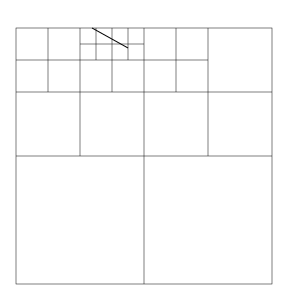
\includegraphics[width=5cm]{images/meshes/AMR/amr4}
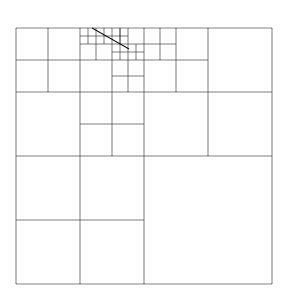
\includegraphics[width=5cm]{images/meshes/AMR/amr5}\\
\includegraphics[width=5cm]{images/meshes/AMR/amr6}
\includegraphics[width=5cm]{images/meshes/AMR/amr7}
\includegraphics[width=5cm]{images/meshes/AMR/amr8}

\begin{tabular}{l|ccccccccc}
             & \# l0  & \# l1 & \# l2 & \# l3 & \# l4 & \# l5 & \# l6 & \# l7 & \# l8 \\ 
\hline\hline
max level= 0 & 1 & \\
max level= 1 & 0 & 4 & \\
max level= 2 & 0 & 3 & 4 \\
max level= 3 & 0 & 2 & 7 & 4\\
max level= 4 & 0 & 2 & 5 & 10 & 8 \\
max level= 5 & 0 & 1 & 8 & 12 & 11 & 20 \\ 
max level= 6 & 0 & 1 & 8 & 11 & 13 & 20 & 32 \\
max level= 7 & 0 & 0 & 11 & 14 & 15 & 23 & 37 & 60 \\
max level= 8 & 0 & 0 & 11 & 13 & 17 & 27 & 43 & 72 & 116 \\
\hline
\end{tabular}

\includegraphics[width=8cm]{images/meshes/AMR/amr_data1.pdf}
\includegraphics[width=8cm]{images/meshes/AMR/amr_data2.pdf}

In the particular case presented here, even though the inclusion in a short 
two-dimensional line, the total number of elements grows faster than the 
third power of the refinement level. While of course the total number 
of elements remains much smaller than the constant resolution counterpart, 
this observation tells us that authorising a unit increase of the maximum 
refinement level can have a substantial effect on the total number of elements.

\newpage

\noindent
\includegraphics[width=4cm]{images/meshes/AMR/amr_0}
\includegraphics[width=4cm]{images/meshes/AMR/amr_1}
\includegraphics[width=4cm]{images/meshes/AMR/amr_2}
\includegraphics[width=4cm]{images/meshes/AMR/amr_3}\\
\includegraphics[width=4cm]{images/meshes/AMR/amr_4}
\includegraphics[width=4cm]{images/meshes/AMR/amr_5}
\includegraphics[width=4cm]{images/meshes/AMR/amr_6}
\includegraphics[width=4cm]{images/meshes/AMR/amr_7}


\includegraphics[width=5cm]{images/meshes/AMR/amr_data3.pdf}
\includegraphics[width=5cm]{images/meshes/AMR/amr_data4.pdf}
\includegraphics[width=5cm]{images/meshes/AMR/amr_data5.pdf}






%.......................................
\subsubsection{Conformal Mesh Refinement}

\Literature: \cite{vaks15}\cite{kott05}


%.......................................
\subsubsection{Meshes in an annulus}


\begin{center}
\includegraphics[width=7cm]{images/meshes/brhv08}
\includegraphics[width=7cm]{images/meshes/brva07a}\\
{\scriptsize The quadratic finite element mesh as used in \cite{brhv08,brva07a}}
\end{center}


%.......................................
\subsubsection{Meshes in a hollow sphere}

The cubed sphere \cite{roip96}

The Citcom mesh  \cite{thie18}

WRITE MORE!!
 %----------------------------
\newpage %-----------------------------------------------------------------------------------------
\subsection{Visco-Plasticity} 
\Literature: \cite{mumc03,chpe15,momu06,muso11}

\subsubsection{Tensor invariants}\label{sec:invariants}

Before we dive into the world of nonlinear rheologies it is necessary to introduce the concept of tensor 
invariants since they are needed further on. \index{general}{Tensor Invariant}
Unfortunately there are many different notations used in the literature and these can prove to be 
confusing. Note that we only consider symmetric tensors in what follows.

\index{general}{Moment Invariant}
Given a tensor $\bm{T}$,  one can compute its (moment) invariants as follows \cite[p.339]{reddybook2}: 
\begin{itemize}
\item first invariant:
\begin{eqnarray}
{\cal I}_1({\bm T})|^{2D} &=& Tr[\bm{T}] = T_{xx} + T_{yy} \nonumber\\
{\cal I}_1({\bm T})|^{3D} &=& Tr[\bm{T}] = T_{xx} + T_{yy} + T_{zz} 
\end{eqnarray}
\item second invariant:
\begin{eqnarray}
{\cal I}_2({\bm T})|^{2D} &=& \frac{1}{2} Tr[{\bm T}\cdot{\bm T}] = \frac{1}{2} \sum_{ij} T_{ij} T_{ji} = \frac{1}{2} (T_{xx}^2 + T_{yy}^2) + T_{xy}^2 \nonumber\\
{\cal I}_2({\bm T})|^{3D} &=& \frac{1}{2} Tr[{\bm T}\cdot{\bm T}] = \frac{1}{2} \sum_{ij} T_{ij} T_{ji} = \frac{1}{2} (T_{xx}^2 + T_{yy}^2 + T_{yy}^2) + T_{xy}^2 + T_{xz}^2 + T_{yz}^2 
\end{eqnarray}
\item third invariant: 
\begin{equation}
{\cal I}_3({\bm T}) = \frac{1}{3} Tr[{\bm T}\cdot{\bm T}\cdot {\bm T}]  = \frac{1}{3}\sum_i\sum_j \sum_k T_{ij} T_{jk} T_{ki} 
\end{equation}
\end{itemize}
These definitions are to be found in Appendix A.2 of \cite{zita2}.
 

\subsubsection{Stress invariants}\label{sec:stress_invariants}

The implementation of the plasticity criterions relies essentially 
on the second invariants of the (deviatoric) stress ${\bm \tau}$ 
and the (deviatoric) strainrate tensors $\dot{\bm \varepsilon}$:

\begin{eqnarray}
{\cal I}_2({\bm \tau})|^{2D}            
&=& \frac{1}{2} ( \tau_{xx}^2 + \tau_{yy}^2  ) + \tau_{xy}^2   \nonumber\\
&=& \frac{1}{4} (\sigma_{xx} - \sigma_{yy})^2 + \sigma_{xy}^2 \nonumber\\
\nonumber\\
{\cal I}_2({\bm \tau})|^{3D}            
&=&\frac{1}{2}(\tau_{xx}^2 + \tau_{yy}^2 + \tau_{zz}^2 ) + \tau_{xy}^2 + \tau_{xz}^2 + \tau_{yz}^2  \nonumber\\
&=&\frac{1}{6}\left[(\sigma_{xx}-\sigma_{yy})^2 + (\sigma_{yy}-\sigma_{zz})^2 + (\sigma_{xx}-\sigma_{zz})^2 \right] 
   + \sigma_{xy}^2 + \sigma_{xz}^2 + \sigma_{yz}^2 \nonumber \\
\nonumber\\
{\cal I}_2(\dot{\bm{\varepsilon}}^d)|^{2D} 
&=& \frac{1}{2} \left[ (\dot{\varepsilon}_{xx}^d)^2 + (\dot{\varepsilon}_{yy}^d)^2  \right] + (\dot{\varepsilon}_{xy}^d)^2  \nonumber\\
           &=& \frac{1}{2} \left[ 
               \frac{1}{4}(\dot{\varepsilon}_{xx} - \dot{\varepsilon}_{yy})^2 + \frac{1}{4}(\dot{\varepsilon}_{yy} - \dot{\varepsilon}_{xx})^2 
               \right] + \dot{\varepsilon}_{xy}^2  \nonumber\\
           &=& \frac{1}{4} (\dot{\varepsilon}_{xx} - \dot{\varepsilon}_{yy})^2  + \dot{\varepsilon}_{xy}^2  \nonumber\\
\nonumber\\
{\cal I}_2(\dot{\bm{\varepsilon}}^d)|^{3D} 
&=& \frac{1}{2} \left[ (\dot{\varepsilon}_{xx}^d)^2 + (\dot{\varepsilon}_{yy}^d)^2 + (\dot{\varepsilon}_{zz}^d)^2   \right] 
+ (\dot{\varepsilon}_{xy}^d)^2  
+ (\dot{\varepsilon}_{xz}^d)^2  
+ (\dot{\varepsilon}_{yz}^d)^2  \nonumber\\
           &=& \frac{1}{6} \left[ (\dot{\epsilon}_{xx}-\dot{\epsilon}_{yy})^2 + (\dot{\epsilon}_{yy}-\dot{\epsilon}_{zz})^2 + (\dot{\epsilon}_{xx}-\dot{\epsilon}_{zz})^2 \right] 
               + \dot{\epsilon}_{xy}^2 + \dot{\epsilon}_{xz}^2 + \dot{\epsilon}_{yz}^2 \nonumber \\
\nonumber
\end{eqnarray}

Note that these (second) invariants are almost always used under a square root so we define:
\begin{mdframed}[backgroundcolor=blue!5]
\[
\tau_{e}=\sqrt{{\cal I}_2({\bm \tau})}
\quad\quad
\quad\quad
\dot{\varepsilon}_{e}=\sqrt{{\cal I}_2(\dot{\bm \varepsilon}^d)}
\]
\end{mdframed}
Note that these quantities have the same dimensions as their tensor counterparts, i.e. Pa for stresses and s$^{-1}$ for strain rates.

If the stress tensor is such that it is diagonal, i.e.
\[
{\bm \sigma}= \left( \begin{array}{ccc}
\sigma_1 & 0 & 0 \\
0 & \sigma_2 & 0 \\
0 & 0 & \sigma_3
\end{array}\right)
\qquad
{\rm and}
\qquad
{\bm \tau}= \left( \begin{array}{ccc}
\tau_1 & 0 & 0 \\
0 & \tau_2 & 0 \\
0 & 0 & \tau_3
\end{array}\right)
\]
then the invariants are 
\begin{eqnarray}
{\cal I}_1({\bm \sigma}) &=& \sigma_1 + \sigma_2+ \sigma_3 \nonumber\\
{\cal I}_2({\bm \tau})|^{2D} &=& \frac{1}{4} (\sigma_{1} - \sigma_{2})^2 \nonumber\\
{\cal I}_2({\bm \tau})|^{3D} &=& \frac{1}{6}\left[(\sigma_{1}-\sigma_{2})^2 + (\sigma_{2}-\sigma_{3})^2 
+ (\sigma_{1}-\sigma_{3})^2 \right] \\ 
{\cal I}_3({\bm \tau}) 
&=& \frac{1}{3} Tr[{\bm T}\cdot{\bm T}\cdot {\bm T}]  \nn\\
&=& \frac{1}{3} Tr
\left[
\left(
\begin{array}{ccc}
\tau_1 & 0 & 0 \\
0 & \tau_2 & 0 \\
0 & 0 & \tau_3 
\end{array}
\right)
\cdot
\left(
\begin{array}{ccc}
\tau_1 & 0 & 0 \\
0 & \tau_2 & 0 \\
0 & 0 & \tau_3 
\end{array}
\right)
\cdot
\left(
\begin{array}{ccc}
\tau_1 & 0 & 0 \\
0 & \tau_2 & 0 \\
0 & 0 & \tau_3 
\end{array}
\right)
\right] \nn\\
&=&  \frac{1}{3} Tr
\left(
\begin{array}{ccc}
\tau_1^3 & 0 & 0 \\
0 & \tau_2^3 & 0 \\
0 & 0 & \tau_3^3 
\end{array}
\right) \nn\\
&=& \frac{1}{3}(\tau_1^3+\tau_2^3+\tau_3^3) \nn\\
&=&  \frac{1}{3} [ 
(\sigma_1-{\cal I}_1({\bm \sigma})/3)^3+  
(\sigma_2-{\cal I}_1({\bm \sigma})/3)^3+
(\sigma_3-{\cal I}_1({\bm \sigma})/3)^3 ]   \nonumber\\ 
&=&  \frac{1}{3\cdot 27} [ 
(3\sigma_1-{\cal I}_1({\bm \sigma}))^3+  
(3\sigma_2-{\cal I}_1({\bm \sigma}))^3+
(3\sigma_3-{\cal I}_1({\bm \sigma}))^3 ]   \nonumber\\ 
&=& \frac{1}{81}
\left[
(2\sigma_1-\sigma_2-\sigma_3)^3+
(2\sigma_2-\sigma_1-\sigma_3)^3+
(2\sigma_3-\sigma_1-\sigma_2)^3
\right] 
\label{eq:3rdinvb} 
\end{eqnarray}
This formulation of the third invariant of ${\bm \tau}$ is used in \cite{wojc18}.


{\color{gray} 
One can prove that (REF?)\footnote{Near identical equations are to be found at 
\url{https://en.wikipedia.org/wiki/Cauchy_stress_tensor}} 
\begin{eqnarray}
{\cal I}_3({\bm \tau}) 
&=& \frac{1}{27} \left( 2 {\cal I}_1({\bm \sigma})^3 + 
9 {\cal I}_1({\bm \sigma}) {\cal I}_2({\bm \sigma}) 
+27 {\cal I}_3({\bm \sigma})   \right) \nn\\
&=& det ({\bm\tau}) \nn\\
&=& \tau_1 \tau_2\tau_3 \nn\\
\end{eqnarray}

The third (deviatoric) stress invariant is given by: (VERIFY!!)
\begin{eqnarray}
{\cal I}_3({\bm \tau})|^{3D} 
&=&  \frac{1}{3} s_{xx} (s_{xx}^2 + 3  s_{xy}^2   + 3  s_{xz}^2  )     \nonumber\\
&+& \frac{1}{3} s_{yy} (3s_{xy}^2 +  s_{yy}^2   + 3  s_{yz}^2  )     \nonumber\\
&+& \frac{1}{3} s_{zz} ( 3 s_{xz}^2  + 3 s_{yz}^2 +s_{zz}^2)       \nonumber\\
&+& 2   s_{xy} s_{xz} s_{yz}   \nonumber \\
&=& s_1 s_2 s_3 \nonumber
\end{eqnarray}

}

%%%%%%%%%%%%%%%%%%%%%%%%%%%%%%%%%%%%%%%%%%%%%%%%%%%%%%%%%%%%%%%%%%%%%%%%%%%%%%%%%%%%%%%%%%%%%%%%%%%%
\subsubsection{Alternative principal stresses notations}\label{sec:altinv}

The principal stress of the stress tensor ${\bm \sigma}$ are $\sigma_1$, $\sigma_2$
and $\sigma_3$ with $\sigma_1 \geq \sigma_2 \geq \sigma_3$.
Following \cite{wojc18}, we start by stating that the intermediate principal 
stress can always be represented as a linear combination of two other stresses:
\begin{equation}
\sigma_2 = (1-b)\sigma_1 + b \sigma_3
\qquad
{\rm where}
\qquad
b = \frac{\sigma_1-\sigma_2}{\sigma_1-\sigma_3}\in [0,1]
\end{equation}
The quantity $b$ is called the principal stress ratio. \index{general}{Principal Stress Ratio}
Let us now introduce the maximum shear plane stresses $p$ and $q$ such that 
\begin{equation}
p=\frac{\sigma_1+\sigma_3}{2}
\qquad
q=\frac{\sigma_1-\sigma_3}{2}
\end{equation}
so that we have 
\begin{eqnarray}
\sigma_1 &=& p+q \\
\sigma_2 &=& p-aq \qquad a=2b-1 \in[-1,1] \\
\sigma_3 &=& p-q
\end{eqnarray}
The quantity $a$ is an equivalent measure of the principal stress ratio.
We can introduce $a,p,q$ in the invariants above:
\begin{eqnarray}
{\cal I}_1({\bm \sigma}) 
&=& \sigma_1 + \sigma_2 + \sigma_3 \nn\\
&=& p+q + p-aq + p-q \nn\\
&=& 3p -aq \\
{\cal I}_2({\bm \tau}) 
&=&\frac{1}{6}\left[(\sigma_{1}-\sigma_{2})^2 +(\sigma_{2}-\sigma_{3})^2 +(\sigma_{1}-\sigma_{3})^2\right]\nn\\ 
&=&\frac{1}{6}\left[(p+q-p+aq)^2 +(p-aq-p+q)^2 +(p+q-p+q)^2\right]\nn\\ 
&=&\frac{1}{6}\left[(q+aq)^2 +(-aq+q)^2 +(q+q)^2\right]\nn\\ 
&=&\frac{q^2}{6}\left[(1+a)^2 +(-a+1)^2 + 4 \right]\nn\\ 
&=&\frac{q^2}{6}\left[ 1+2a+a^2 +1 - 2a+a^2 + 4 \right]\nn\\ 
&=&\frac{q^2}{3}\left( a^2 +3 \right)
\end{eqnarray}
Using the definition of the third invariant of Eq.~\ref{eq:3rdinvb}:
\begin{eqnarray}
{\cal I}_3({\bm \tau}) 
&=& \frac{1}{81} \left[
(2\sigma_1-\sigma_2-\sigma_3)^3+
(2\sigma_2-\sigma_1-\sigma_3)^3+
(2\sigma_3-\sigma_1-\sigma_2)^3
\right] \nn\\
&=& \frac{1}{81} \left[
(2p+2q-p+aq-p+q)^3+
(2p-2aq-p-q-p+q)^3+
(2p-2q-p-q-p+aq)^3
\right] \nn\\
&=& \frac{1}{81} \left[ (2q+aq+q)^3+ (-2aq-q+q)^3+ (-2q-q+aq)^3 \right] \nn\\
&=& \frac{q^3}{81} \left[ (3+a)^3+ (-2a)^3+ (-3+a)^3 \right] \nn\\
&=& \frac{q^3}{81} \left[ 27 +9a + 3a^2 + a^3  -8a^3 -27 +9a -3a^2 + a^3 \right] \nn\\
&=& \frac{q^3}{81} \left( 18a  -6 a^3  \right) \nn\\
&=& \frac{2a q^3}{27} \left( 3 - a^2  \right) 
\end{eqnarray}
which is not exactly Eq.(14) of \cite{wojc18}!!

\begin{remark}
Wojciechowski \cite{wojc18} defines the Lode angle \index{general}{Lode Angle} 
as being the opposite of my definition in Eq.~\ref{eq:lodang}.
\end{remark}

Finally, we can show that 
\begin{eqnarray}
a 
&=& 2b-1 \nn\\
&=& 2 \frac{\sigma_1-\sigma_2}{\sigma_1-\sigma_3} -1 \nn\\
&=& 2 \frac{  -\frac{1}{\sqrt{3}}\sin \theta  + \cos \theta - \frac{2}{\sqrt{3}} \sin \theta }
{-\frac{1}{\sqrt{3}}\sin \theta  + \cos \theta +\frac{1}{\sqrt{3}}\sin \theta  + \cos \theta } -1 \nn\\
&=& \frac{ -\frac{1}{\sqrt{3}}\sin \theta  + \cos \theta - \frac{2}{\sqrt{3}}\sin\theta }{\cos \theta } -1 \nn\\
&=& -\frac{3}{\sqrt{3}} \frac{\sin\theta}{\cos\theta} \nn\\
&=& -\sqrt{3} \tan\theta
\end{eqnarray}
Here again we arrive at the opposite of Eq.16 of \cite{wojc18}. 

%%%%%%%%%%%%%%%%%%%%%%%%%%%%%%%%%%%%%%%%%%%%%%%%%%%%%%%%%%%%%%%%%%%%%%%%%%%%%%%%%%%%%%%%%%%%%%%%%%%%
\subsubsection{Scalar viscoplasticity}

This formulation is quite easy to implement. It is widely used, e.g. \cite{will92,thfb08,spmw16}, and relies on the assumption that 
a scalar quantity $\eta_p$ (the 'effective plastic viscosity') exists such that the deviatoric stress tensor 
\begin{equation}
{\bm \tau}=2\eta_p \dot{\bm\varepsilon} \label{eqscpl1}
\end{equation}
is bounded by some yield stress value $Y$.
From Eq. (\ref{eqscpl1}) it follows that $\underline{\tau}_{II}= 2\eta_p \dot{\underline{\varepsilon}}_{II}=Y$ which yields
\begin{mdframed}[backgroundcolor=blue!5]
\[
\eta_p = \frac{Y}{2 \dot{\underline{\varepsilon}}_{II}}
\]
\end{mdframed}
This approach has also been coined the Viscosity Rescaling Method (VRM) \cite{kacha04}. 
\index{general}{VRM} \index{general}{Viscosity Rescaling Method}

\improvement[inline]{insert here the rederivation 2.1.1 of spmw16}

It is at this stage important to realise that (i) in areas where the strainrate is low, the resulting effective viscosity will be large, and 
(ii) in areas where the strainrate is high, the resulting effective viscosity will be low. This is not without consequences since 
(effective) viscosity contrasts up to 8-10 orders of magnitude have been observed/obtained with this formulation and it makes the FE 
matrix very stiff, leading to (iterative) solver convergence issues.
In order to contain these viscosity contrasts one usually resorts to viscosity limiters $\eta_{min}$ and $\eta_{max}$ such that 
\[
\eta_{min} \leq \eta_p \leq \eta_{max}
\]
Caution must be taken when choosing both values as they may influence the final results.


\begin{mdframed}[backgroundcolor=green!5]
\begin{itemize}
\item[$\triangleright$] {\sl python\_codes/fieldstone\_indentor}
\end{itemize}
\end{mdframed}


%-------------------------------------------------
\subsubsection{About the yield stress value $Y$}

In geodynamics the yield stress value is often given as a simple function. 
It can be constant (in space and time) and in this case we are dealing with a von Mises plasticity yield criterion. 
\index{general}{von Mises}. We simply assume $Y_{vM}=C$ where $C$ is a constant cohesion independent of pressure, strainrate,
deformation history, etc ... \index{general}{Cohesion}

Another model is often used: the Drucker-Prager plasticity model. \index{general}{Drucker-Prager}
A friction angle $\phi$ is then introduced and the yield value $Y$ takes the form
\[
Y_{DP}=p \sin\phi + C \cos \phi
\]
and therefore depends on the pressure $p$. Because $\phi$ is with the range $[0^\circ,45^\circ]$, $Y$ is
found to increase with depth (since the lithostatic pressure often dominates the overpressure).

Note that a slightly modified verion of this plasticity model has been used: the total pressure $p$
is then replaced by the lithostatic pressure $p_{lith}$.




%-------------------------------------------------
\subsubsection{Work in progress}

\Literature \cite{zico74,zigo74,zico74b,zien75,corm75,zigo75,zihl75,zijo78,vidm82,vidm84,vede84,zivt85,vimd86}
\cite{wasd97,debo88,debo01,hesd02,bewv11,mumg10,leor89,sccm13,desm93,demu92,debo91,shmv16}
\cite{modm01}\cite{baji02}
\cite{modm02}

Note that \cite{vidm82,vidm84,vimd86,zivt85} use the following formulation which they attribute to \cite{zijo78}:
\[
\eta_{eff} = \frac{c + (\dot{\varepsilon}_e / \gamma)^{1/n}}{ \dot{\varepsilon}_e }
\] 
For a perfectly plastic flow law, $\gamma \rightarrow \infty$ and then 
\[
\eta_{eff} = \frac{c}{ \dot{\varepsilon}_e }
\] 
and when when $c=0$ then the effective viscosity is essentially of the power law type.
Also, when $n=1$ the formulation becomes identical to the v-vp formulation (when the max viscosity is infinite) and with $1/\gamma=\eta_{min}$.





 %--------------------------------------------
\newpage %-----------------------------------------------------------------------------------------
\subsection{Pressure smoothing/filtering for $Q_1\times P_0$ elements \label{psmoothing}} 
It has been widely documented that the use of the $Q_1 \times P_0$ element is 
not without problems. Aside from the 
consequences it has on the FE matrix properties, we will here focus on another unavoidable side effect: 
the spurious pressure checkerboard modes. 
\index{general}{Pressure Smoothing} 
\index{general}{Checkerboard mode}

These modes have been thoroughly analysed decades ago, see for instance
Hughes \etal (1979)\cite{hulb79}, 
Sani \etal (1981) \cite{sagl81a,sagl81b},
Griffiths \& Silvester (1994) \cite{grsi94}.
They can be filtered out(Chen (1995)  \cite{chpc95}) 
or simply smoothed (Lee \etal (1979) \cite{legs79}), as we will see later.
Nodes on edges and corners may need special treatment as documented in Sani \etal \cite{sagl81a} or
Lee \etal (1979) \cite{legs79}.
The list of 8 schemes is not exhaustive with regards to the above mentioned publications. 
There has been considerable amount of work on the topic and this section is 
unfortunately not representing the literature appropriately.

\mscthesis: Get relevant literature, digest it, implement all variants in \stone 12.
 \index{general}{MSc Thesis} 


On the following figure (a,b), pressure fields for the lid driven cavity experiment 
are presented for both an even and un-even number of elements. We see that 
the amplitude of the modes can sometimes be so large that the 'real' pressure signal is 
not visible under the checkerboard and that something as simple as the number of elements in the 
domain can trigger those or not at all.

\begin{center}
a)\includegraphics[width=4cm]{images/checkerboard/p_el}
\includegraphics[width=4cm]{images/checkerboard/p_el_33x33}
b)\includegraphics[width=5cm]{images/checkerboard/press_doneahuerta}
c)\includegraphics[width=7cm]{images/checkerboard/douarpunch}\\
{\captionfont a) element pressure for a 32x32 grid and for a 33x33 grid;\\ 
b) image from \cite[p307]{dohu03} for a manufactured solution;
c) elemental pressure and smoothed pressure for the punch experiment \cite{thfb08}}
\end{center}

%----------------------------------------------------------------------
\paragraph{Scheme 1}.

The easiest post-processing step that can be used (especially when a regular grid is used) 
is explained in Thieulot \etal (2008) \cite{thfb08}: "The element-to-node interpolation is performed by
averaging the elemental values from elements common to each node; 
the node-to-element interpolation is performed
by averaging the nodal values element-by-element. This
method is not only very efficient but produces a smoothing
of the pressure that is adapted to the local density of the
octree. Note that these two steps can be repeated until a
satisfying level of smoothness (and diffusion) of the pressure field is attained."


\begin{center}
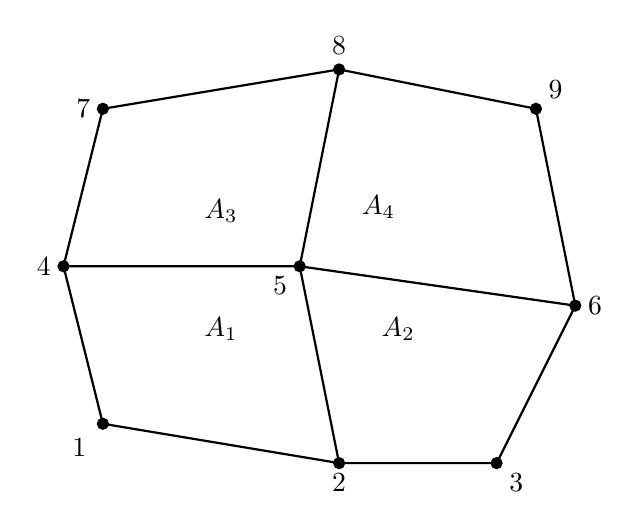
\begin{tikzpicture}
%\draw[fill=gray!5,gray!5](0,0) rectangle (9,7);
%\draw[step=0.5cm,gray,very thin] (0,0) grid (9,7); %background grid
\draw[thick](1.5,1.5) -- (4.5,1) -- (6.5,1) -- (7.5,3) -- (7,5.5) -- (4.5,6) --(1.5,5.5) -- (1,3.5) -- cycle;  
\draw[thick](4.5,1)--(4,3.5)--(4.5,6);
\draw[thick](1,3.5)--(4,3.5)--(7.5,3);
\draw[black,fill=black] (1.5,1.5) circle (2pt); \node[] at (1.2,1.2){1}; %1
\draw[black,fill=black] (4.5,1)   circle (2pt); \node[] at (4.5,0.75){2}; %2
\draw[black,fill=black] (6.5,1)   circle (2pt); \node[] at (6.75,0.75){3}; %3
\draw[black,fill=black] (1,3.5)   circle (2pt); \node[] at (0.75,3.5){4}; %4
\draw[black,fill=black] (4,3.5)   circle (2pt); \node[] at (3.75,3.25){5}; %5
\draw[black,fill=black] (7.5,3)   circle (2pt); \node[] at (7.75,3){6}; %6
\draw[black,fill=black] (1.5,5.5) circle (2pt); \node[] at (1.25,5.5){7}; %7
\draw[black,fill=black] (4.5,6)   circle (2pt); \node[] at (4.5,6.3){8}; %8
\draw[black,fill=black] (7,5.5)   circle (2pt); \node[] at (7.25,5.75){9}; %9
%\draw[thin,dashed](1,3.5)--(4.5,1)--(7.5,3)--(4.5,6)--cycle;
\node[] at (3,2.7){$A_1$}; %8
\node[] at (5.25,2.7){$A_2$}; %8
\node[] at (5,4.25){$A_4$}; %8
\node[] at (3,4.2){$A_3$}; %8
\end{tikzpicture}
\end{center}
\[
q_5^{(1)} = \frac{1}{4}\sum_{e=1}^4 p_e
\] 

In the codes which rely on the $Q_1 \times P_0$ element, the (elemental) pressure
is simply defined as 
\begin{lstlisting}
p=np.zeros(nel,dtype=np.float64)  
\end{lstlisting}
while the nodal pressure is then defined as\footnote{In virtually all stones $p$
stands for the 'raw' pressure and $q$ stands for its projection onto the velocity mesh.} 
\begin{lstlisting}
q=np.zeros(nnp,dtype=np.float64)  
\end{lstlisting}
The element-to-node algorithm is then simply (in 2D):

\begin{lstlisting}
count=np.zeros(nnp,dtype=np.int32)  
for iel in range(0,nel):
    q[icon[0,iel]]+=p[iel]
    q[icon[1,iel]]+=p[iel]
    q[icon[2,iel]]+=p[iel]
    q[icon[3,iel]]+=p[iel]
    count[icon[0,iel]]+=1
    count[icon[1,iel]]+=1
    count[icon[2,iel]]+=1
    count[icon[3,iel]]+=1
q=q/count
\end{lstlisting}



%----------------------------------------------------------------------
\paragraph{Schemes 2,3}.

{\sl Schemes 2,3} are very similar and are presented in Sani \etal (1981) \cite{sagl81a,sagl81b}.
Scheme 2 uses the areas of the surrounding elements as weights for the arithmetic averaging
while scheme 3 uses the area of the triangles:

\begin{multicols}{2}

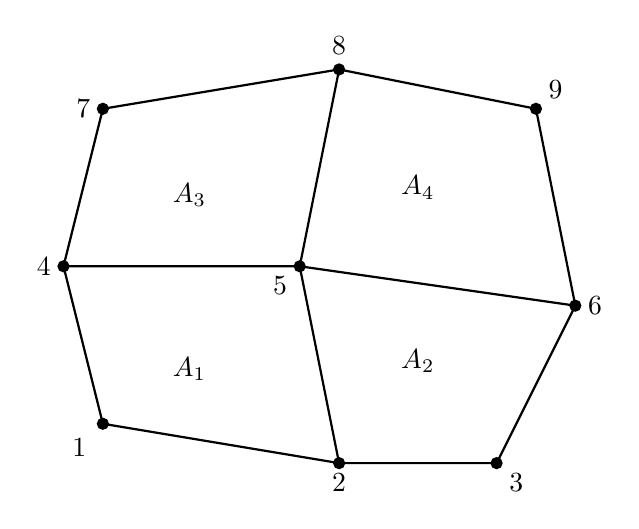
\begin{tikzpicture}
%\draw[fill=gray!5,gray!5](0,0) rectangle (9,7);
%\draw[step=0.5cm,gray,very thin] (0,0) grid (9,7); %background grid
\draw[thick](1.5,1.5) -- (4.5,1) -- (6.5,1) -- (7.5,3) -- (7,5.5) -- (4.5,6) --(1.5,5.5) -- (1,3.5) -- cycle;  
\draw[thick](4.5,1)--(4,3.5)--(4.5,6);
\draw[thick](1,3.5)--(4,3.5)--(7.5,3);
\draw[black,fill=black] (1.5,1.5) circle (2pt); \node[] at (1.2,1.2){1}; %1
\draw[black,fill=black] (4.5,1)   circle (2pt); \node[] at (4.5,0.75){2}; %2
\draw[black,fill=black] (6.5,1)   circle (2pt); \node[] at (6.75,0.75){3}; %3
\draw[black,fill=black] (1,3.5)   circle (2pt); \node[] at (0.75,3.5){4}; %4
\draw[black,fill=black] (4,3.5)   circle (2pt); \node[] at (3.75,3.25){5}; %5
\draw[black,fill=black] (7.5,3)   circle (2pt); \node[] at (7.75,3){6}; %6
\draw[black,fill=black] (1.5,5.5) circle (2pt); \node[] at (1.25,5.5){7}; %7
\draw[black,fill=black] (4.5,6)   circle (2pt); \node[] at (4.5,6.3){8}; %8
\draw[black,fill=black] (7,5.5)   circle (2pt); \node[] at (7.25,5.75){9}; %9
\node[] at (2.6,2.2){$A_1$}; %8
\node[] at (5.5,2.3){$A_2$}; %8
\node[] at (2.6,4.4){$A_3$}; %8
\node[] at (5.5,4.5){$A_4$}; %8
\end{tikzpicture}

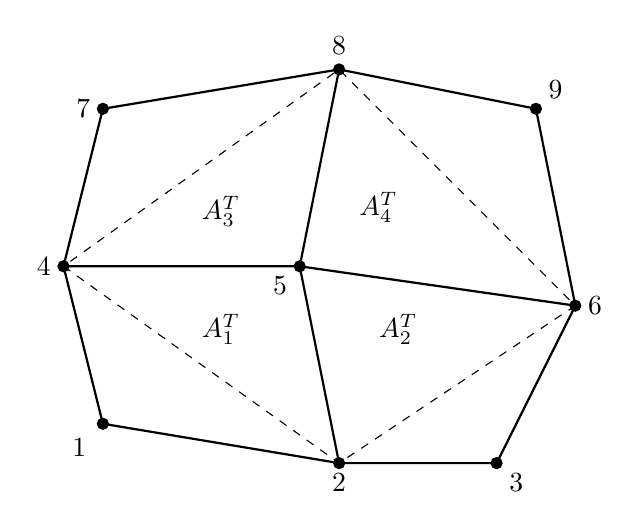
\begin{tikzpicture}
%\draw[fill=gray!5,gray!5](0,0) rectangle (9,7);
%\draw[step=0.5cm,gray,very thin] (0,0) grid (9,7); %background grid
\draw[thick](1.5,1.5) -- (4.5,1) -- (6.5,1) -- (7.5,3) -- (7,5.5) -- (4.5,6) --(1.5,5.5) -- (1,3.5) -- cycle;  
\draw[thick](4.5,1)--(4,3.5)--(4.5,6);
\draw[thick](1,3.5)--(4,3.5)--(7.5,3);
\draw[black,fill=black] (1.5,1.5) circle (2pt); \node[] at (1.2,1.2){1}; %1
\draw[black,fill=black] (4.5,1)   circle (2pt); \node[] at (4.5,0.75){2}; %2
\draw[black,fill=black] (6.5,1)   circle (2pt); \node[] at (6.75,0.75){3}; %3
\draw[black,fill=black] (1,3.5)   circle (2pt); \node[] at (0.75,3.5){4}; %4
\draw[black,fill=black] (4,3.5)   circle (2pt); \node[] at (3.75,3.25){5}; %5
\draw[black,fill=black] (7.5,3)   circle (2pt); \node[] at (7.75,3){6}; %6
\draw[black,fill=black] (1.5,5.5) circle (2pt); \node[] at (1.25,5.5){7}; %7
\draw[black,fill=black] (4.5,6)   circle (2pt); \node[] at (4.5,6.3){8}; %8
\draw[black,fill=black] (7,5.5)   circle (2pt); \node[] at (7.25,5.75){9}; %9
\draw[thin,dashed](1,3.5)--(4.5,1)--(7.5,3)--(4.5,6)--cycle;
\node[] at (3,2.7){$A_1^T$}; %8
\node[] at (5.25,2.7){$A_2^T$}; %8
\node[] at (5,4.25){$A_4^T$}; %8
\node[] at (3,4.2){$A_3^T$}; %8
\end{tikzpicture}

\end{multicols}




\[
q_5^{(2)} = \frac{\sum\limits_{e=1}^4 A_e p_e}{\sum\limits_{e=1}^4 A_e}
\qquad
\qquad
q_5^{(3)} = \frac{\sum\limits_{e=1}^4 A_e^T p_e}{\sum\limits_{e=1}^4 A_e^T}
\] 


\begin{remark} Although Schemes 1,2,3 are similar, scheme 1 is the simplest and fastest
to implement since the areas of neighbouring elements/triangles are not needed.
\end{remark}

\begin{remark} 
Schemes 1,2,3 are identical if all elements are rectangles of identical dimensions.
\end{remark}




%----------------------------------------------------------------------
\paragraph{Scheme 4} This scheme has been designed by me. 
It resembles the last three ones, but the weighing is in this case different.

Let us consider a 1D problem:
\begin{center}
\includegraphics[width=0.5\linewidth]{images/pressure_smoothing/newalgo.png}
\end{center}

Elemental pressures $p_1$ and $p_2$ corresponding to elements 1 and 2 respectively are known at
locations $x_1$ and $x_2$. The two elements have a different size, characterised in this case
by the distances $d_1$ and $d_2$ to their common edge.

The equation of the line passing through points $(x_1,p_1)$ and $(x_2,p_2)$ is 
\[
p(x)=\frac{p_2-p_1}{x_2-x_1}(x-x_1)+p_1
\]
The $x$ coordinate of the common edge is given by $x=x_1+d_1/2$, 
and since $x_2-x_1=(d_1+d_2)/2$, the 
pressure at this location writes:
\[
p(x_M)= \frac{p_2-p_1}{d_1+d_2}d_1+p_1 = \frac{\frac{p_1}{d_1} + \frac{p_2}{d_2}}{\frac{1}{d_1} + \frac{1}{d_2}}
\]
Extrapolating this formula to 2D, $d_1$ and $d_2$ are in fact the element volumes, so that
\[
q_5^{(4)} = 
\frac{\sum\limits_{j=1}^4 \frac{p_j^e}{A_j^e}}{\sum\limits_{j=1}^4 \frac{1}{A_j^e}}
=
\frac{
\frac{p_1^e}{A_1^e}+
\frac{p_2^e}{A_2^e}+
\frac{p_3^e}{A_3^e}+
\frac{p_4^e}{A_4^e}
}{
\frac{1}{A_1^e}+
\frac{1}{A_2^e}+
\frac{1}{A_3^e}+
\frac{1}{A_4^e}
}\]

There remains a problem, due to the presence of the boundary nodes for which 
the sums present in the above equation do not run up to 4. A boundary
node only has three neighbours and a corner node only two. Additional measures
are required for these nodes. 

\begin{center}
\includegraphics[width=0.5\linewidth]{images/pressure_smoothing/newalgo_corner.png}
\end{center}

The pressure value $p_N$ is obtained as follows:
\[
q_N = \frac{ 
 \frac{p_2^e}   {A_2^e}
+\frac{p_3^e}   {A_3^e}
+\frac{p_{2'}^e}{A_{2'}^e}
+\frac{p_{3'}^e}{A_{3'}^e}
}{
 \frac{1}{A_2^e}
+\frac{1}{A_3^e}
+\frac{1}{A_{2'}^e}
+\frac{1}{A_{3'}^e}
}
\]
The areas and pressures of the mirrored elements 2' and 3' are extrapolated from the areas of elements 2 and 6, and 3 and 7 respectively. 
Likewise the pressure $p_M$ at the corner node is obtained through the pressures of its surrounding elements.


%------------------------------------------------------------------------------
\paragraph{Scheme 5 - Least squares} This scheme is presented (among other places) in Lee \etal (1979)
\cite{legs79}. 
Let us start from the patch of 4 $Q_1$ elements counting 9 nodes: 

\begin{center}
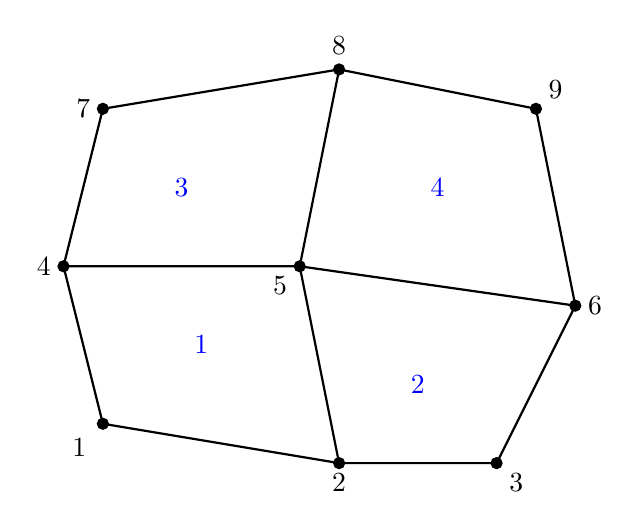
\begin{tikzpicture}
%\draw[fill=gray!5,gray!5](0,0) rectangle (9,7);
%\draw[step=0.5cm,gray,very thin] (0,0) grid (9,7); %background grid
\draw[thick](1.5,1.5) -- (4.5,1) -- (6.5,1) -- (7.5,3) -- (7,5.5) -- (4.5,6) --(1.5,5.5) -- (1,3.5) -- cycle;  
\draw[thick](4.5,1)--(4,3.5)--(4.5,6);
\draw[thick](1,3.5)--(4,3.5)--(7.5,3);

\node[] at (2.75,2.5) {\color{blue}1};
\node[] at (5.5,2) {\color{blue}2};
\node[] at (2.5,4.5) {\color{blue}3};
\node[] at (5.75,4.5) {\color{blue}4};

\draw[black,fill=black] (1.5,1.5) circle (2pt); \node[] at (1.2,1.2){1}; %1
\draw[black,fill=black] (4.5,1)   circle (2pt); \node[] at (4.5,0.75){2}; %2
\draw[black,fill=black] (6.5,1)   circle (2pt); \node[] at (6.75,0.75){3}; %3
\draw[black,fill=black] (1,3.5)   circle (2pt); \node[] at (0.75,3.5){4}; %4
\draw[black,fill=black] (4,3.5)   circle (2pt); \node[] at (3.75,3.25){5}; %5
\draw[black,fill=black] (7.5,3)   circle (2pt); \node[] at (7.75,3){6}; %6
\draw[black,fill=black] (1.5,5.5) circle (2pt); \node[] at (1.25,5.5){7}; %7
\draw[black,fill=black] (4.5,6)   circle (2pt); \node[] at (4.5,6.3){8}; %8
\draw[black,fill=black] (7,5.5)   circle (2pt); \node[] at (7.25,5.75){9}; %9

\end{tikzpicture}
\end{center}



We are looking for a field $q$ living on the nodes.
We build the quantity
\[
J=\iint_\Omega (q-p)^2 dV
\]
where $p$ is the elemental field. To make things clearer we split the integral into 
the sum of elemental integrals:
\[
J=
\iint_{\Omega_1} (q(x,y)-p_1)^2 dV+
\iint_{\Omega_2} (q(x,y)-p_2)^2 dV+
\iint_{\Omega_3} (q(x,y)-p_3)^2 dV+
\iint_{\Omega_4} (q(x,y)-p_4)^2 dV
\]
Inside each element the field $q(x,y)$ is given by a bilinear interpolation so that:
\begin{eqnarray}
J
&=& \iint_{\Omega_1} (\bN_1(x,y) q_1 + \bN_2(x,y)q_2 + \bN_5(x,y)q_5 + \bN_4(x,y)q_4 -p_1)^2 dV \nn\\
&+& \iint_{\Omega_2} (\bN_2(x,y) q_2 + \bN_3(x,y)q_3 + \bN_6(x,y)q_6 + \bN_5(x,y)q_5 -p_2)^2 dV \nn\\
&+& \iint_{\Omega_3} (\bN_4(x,y) q_4 + \bN_5(x,y)q_5 + \bN_8(x,y)q_8 + \bN_7(x,y)q_7 -p_3)^2 dV \nn\\
&+& \iint_{\Omega_4} (\bN_5(x,y) q_5 + \bN_6(x,y)q_6 + \bN_9(x,y)q_9 + \bN_8(x,y)q_8 -p_4)^2 dV 
\end{eqnarray}
where the $N_i$ functions are the basis functions (unusually expressed in $x,y$ coordinates).
The least square procedure looks for the set of $q_i$ such that 
\[
\frac{\partial J}{\partial q_i} =0 \qquad \forall i=1,...9
\]
and this yields 9 equations/constraints for 9 unknowns.
\begin{eqnarray}
\frac{\partial J}{\partial q_1} 
&=& \iint_{\Omega_1} 2 (\bN_1(x,y) q_1 + \bN_2(x,y)q_2 + \bN_5(x,y)q_5 + \bN_4(x,y)q_4 -p_1) \bN_1(x,y) dV \nn\\
\frac{\partial J}{\partial q_2}
&=& \iint_{\Omega_1} 2(\bN_1(x,y) q_1 + \bN_2(x,y)q_2 + \bN_5(x,y)q_5 + \bN_4(x,y)q_4 -p_1) \bN_2(x,y) dV \nn\\
&+& \iint_{\Omega_2} 2(\bN_2(x,y) q_2 + \bN_3(x,y)q_3 + \bN_6(x,y)q_6 + \bN_5(x,y)q_5 -p_2) \bN_2(x,y) dV \nn\\
\frac{\partial J}{\partial q_3}
&=& \iint_{\Omega_2} 2(\bN_2(x,y) q_2 + \bN_3(x,y)q_3 + \bN_6(x,y)q_6 + \bN_5(x,y)q_5 -p_2) \bN_3(x,y) dV \nn\\
\frac{\partial J}{\partial q_4}
&=& \iint_{\Omega_1} 2(\bN_1(x,y) q_1 + \bN_2(x,y)q_2 + \bN_5(x,y)q_5 + \bN_4(x,y)q_4 -p_1) \bN_4(x,y) dV \nn\\
&+& \iint_{\Omega_3} 2(\bN_4(x,y) q_4 + \bN_5(x,y)q_5 + \bN_8(x,y)q_8 + \bN_7(x,y)q_7 -p_3) \bN_4(x,y) dV \nn\\
\frac{\partial J}{\partial q_5}
&=& \iint_{\Omega_1} 2(\bN_1(x,y) q_1 + \bN_2(x,y)q_2 + \bN_5(x,y)q_5 + \bN_4(x,y)q_4 -p_1) \bN_5(x,y) dV \nn\\
&+& \iint_{\Omega_2} 2(\bN_2(x,y) q_2 + \bN_3(x,y)q_3 + \bN_6(x,y)q_6 + \bN_5(x,y)q_5 -p_2) \bN_5(x,y) dV \nn\\
&+& \iint_{\Omega_3} 2(\bN_4(x,y) q_4 + \bN_5(x,y)q_5 + \bN_8(x,y)q_8 + \bN_7(x,y)q_7 -p_3) \bN_5(x,y) dV \nn\\
&+& \iint_{\Omega_4} 2(\bN_5(x,y) q_5 + \bN_6(x,y)q_6 + \bN_9(x,y)q_9 + \bN_8(x,y)q_8 -p_4) \bN_5(x,y) dV \nn\\
\frac{\partial J}{\partial q_6}
&=& \iint_{\Omega_2} 2(\bN_2(x,y) q_2 + \bN_3(x,y)q_3 + \bN_6(x,y)q_6 + \bN_5(x,y)q_5 -p_2) \bN_6(x,y) dV \nn\\
&+& \iint_{\Omega_4} 2(\bN_5(x,y) q_5 + \bN_6(x,y)q_6 + \bN_9(x,y)q_9 + \bN_8(x,y)q_8 -p_4) \bN_6(x,y) dV \nn\\
\frac{\partial J}{\partial q_7}
&=& \iint_{\Omega_3} 2(\bN_4(x,y) q_4 + \bN_5(x,y)q_5 + \bN_8(x,y)q_8 + \bN_7(x,y)q_7 -p_3) \bN_7(x,y) dV \nn\\
\frac{\partial J}{\partial q_8}
&=& \iint_{\Omega_3} 2(\bN_4(x,y) q_4 + \bN_5(x,y)q_5 + \bN_8(x,y)q_8 + \bN_7(x,y)q_7 -p_3) \bN_8(x,y)dV \nn\\
&+& \iint_{\Omega_4} 2(\bN_5(x,y) q_5 + \bN_6(x,y)q_6 + \bN_9(x,y)q_9 + \bN_8(x,y)q_8 -p_4) \bN_8(x,y)dV \nn\\ 
\frac{\partial J}{\partial q_9}
&=& \iint_{\Omega_4} 2(\bN_5(x,y) q_5 + \bN_6(x,y)q_6 + \bN_9(x,y)q_9 + \bN_8(x,y)q_8 -p_4) \bN_9(x,y)dV 
\end{eqnarray}
The factor 2 are removed and the terms $\int p_i N_j $ are known so they end up in the right hand side.
\begin{eqnarray}
 \iint_{\Omega_1} (\bN_1 \bN_1 q_1 + \bN_1 \bN_2 q_2 + \bN_1 \bN_5 q_5 + \bN_1 \bN_4 q_4) dV 
&=& \iint_{\Omega_1} p_1 N_1 dV \nn\\
 \iint_{\Omega_1} (\bN_2 \bN_1 q_1 + \bN_2 \bN_2 q_2 + \bN_2 \bN_5 q_5 + \bN_2 \bN_4 q_4) dV \nn\\
+\iint_{\Omega_2} (\bN_2 \bN_2 q_2 + \bN_3 \bN_2 q_3 + \bN_6 \bN_2 q_6 + \bN_5 \bN_2 q_5) dV 
&=& \iint_{\Omega_1} p_1N_2 dV + \iint_{\Omega_2}  p_2 \bN_2 dV \nn\\
\nn\\
\dots &=& \dots \nn\\
\nn\\
 \iint_{\Omega_4} (\bN_9\bN_5 q_5 + \bN_9\bN_6q_6 + \bN_9\bN_9q_9 + \bN_9\bN_8q_8) dV &=&  \iint_{\Omega_4} p_4 \bN_9 dV 
\end{eqnarray}

The mass matrices corresponding to the four elements are 
\[
{\bm M}_1 = \int_{\Omega_1} \left( \begin{array}{cccc}
 \bN_1 \bN_1 & \bN_1 \bN_2 & \bN_1 \bN_5 & \bN_1 \bN_4 \\
 \bN_2 \bN_1 & \bN_2 \bN_2 & \bN_2 \bN_5 & \bN_2 \bN_4 \\
 \bN_5 \bN_1 & \bN_5 \bN_2 & \bN_5 \bN_5 & \bN_5 \bN_4 \\
 \bN_4 \bN_1 & \bN_4 \bN_2 & \bN_4 \bN_5 & \bN_4 \bN_4 
\end{array}\right) dV
\qquad
{\bm M}_2 = \int_{\Omega_2} \left( \begin{array}{cccc}
 \bN_2 \bN_2 & \bN_2 \bN_3 & \bN_2 \bN_6 & \bN_2 \bN_5 \\
 \bN_3 \bN_2 & \bN_3 \bN_3 & \bN_3 \bN_6 & \bN_3 \bN_5 \\
 \bN_6 \bN_2 & \bN_6 \bN_3 & \bN_6 \bN_6 & \bN_6 \bN_5 \\
 \bN_5 \bN_2 & \bN_5 \bN_3 & \bN_5 \bN_6 & \bN_5 \bN_5 
\end{array}\right) dV
\]
\[
{\bm M}_3 = \int_{\Omega_3} \left( \begin{array}{cccc}
 \bN_4 \bN_4 & \bN_4 \bN_5 & \bN_4 \bN_8 & \bN_4 \bN_7 \\
 \bN_5 \bN_4 & \bN_5 \bN_5 & \bN_5 \bN_8 & \bN_5 \bN_7 \\
 \bN_8 \bN_4 & \bN_8 \bN_5 & \bN_8 \bN_8 & \bN_8 \bN_7 \\
 \bN_7 \bN_4 & \bN_7 \bN_5 & \bN_7 \bN_8 & \bN_7 \bN_7 
\end{array}\right) dV
\qquad
{\bm M}_4 = \int_{\Omega_4} \left( \begin{array}{cccc}
 \bN_5 \bN_5 & \bN_5 \bN_6 & \bN_5 \bN_9 & \bN_5 \bN_8 \\
 \bN_6 \bN_5 & \bN_6 \bN_6 & \bN_6 \bN_9 & \bN_6 \bN_8 \\
 \bN_9 \bN_5 & \bN_9 \bN_6 & \bN_9 \bN_9 & \bN_9 \bN_8 \\
 \bN_8 \bN_5 & \bN_8 \bN_6 & \bN_8 \bN_9 & \bN_8 \bN_8 
\end{array}\right) dV
\]
so that the 9 equations above are actually the result of the assembly process of these four 
elemental systems:
\[
\left( \iint_{\Omega_e} \vec{\bN}^T\vec{\bN} dV \right) \cdot \vec{q}_e = \iint_{\Omega_i} \vec{\bN}^T p_e dV 
\qquad\qquad e=1,2,3,4
\]


%------------------------------------------------------------------------------
\paragraph{Scheme 6 - Consistent pressure recovery}

The is the method presented in Zienkiewicz \& Nakazawa (1982) \cite{zina82}. In the second part 
of this publication the authors wish to establish a simple and effective numerical method to calculate 
variables eliminated by the penalisation process. 
The method involves an additional finite element solution for the nodal pressures using 
the same finite element basis and numerical quadrature as used for the velocity.

Let us start with\footnote{I here voluntarily use $q$ instead of $p$}:
\[
q = -\lambda \vec\nabla\cdot \vec\upnu
\]
We are going to treat this equation as any other PDE in the context of the FE method, i.e. 
we are going to establish its weak form. 
We assume that the pressure is given inside an element by
\[
q(x,y) = \sum_{i=1}^4 \bN_i(x,y) q_i = \vec{\bN} \cdot \vec{q}
\]
and the velocity:
\[
\vec\upnu = (u,v) 
\qquad 
\qquad 
u(x,y)  = \sum_{i=1}^4 \bN_i(x,y) u_i
\qquad 
\qquad 
v(x,y)  = \sum_{i=1}^4 \bN_i(x,y) v_i
\]
where the $\bN_i$ are the $Q_1$ basis functions and $q_i$ are the sought after nodal values. 
We multiply the equation above by a $Q_1$ basis function $\bN_i$ and integrate over the whole domain:
\[
\iint_\Omega \bN_i(x,y) q(x,y) \; dxdy 
= -\lambda \iint_\Omega \bN_i \vec\nabla\cdot \vec\upnu  \; dx dy
\]
As before we now focus on the above expression inside a single element $e$:
\[
\iint_{\Omega_e} \bN_i(x,y) q(x,y) \; dxdy = -\lambda \iint_{\Omega_e} \bN_i \vec\nabla\cdot \vec\upnu \; dx dy
\]
After $\bN_i \rightarrow \vec{\bN}=(\bN_1,\bN_2,\bN_3,\bN_4)^T$, the left hand side term becomes:
\[
\iint _{\Omega_e} \vec{\bN}^T q(x,y) \; dxdy 
=
\iint _{\Omega_e} \vec{\bN}^T \vec{\bN} \cdot \vec{q} \; dxdy 
=
\left(\underbrace{\iint _{\Omega_e} \vec{\bN}^T \vec{\bN} dxdy}_{{\bm M}_e} \right) \cdot \vec{q}  
\]
where ${\bm M}_e$ is the elemental mass matrix.
We now turn to the right hand side. We have
\[
\vec\nabla\cdot \vec\upnu
= \frac{\partial u}{\partial x}+\frac{\partial v}{\partial y}
= \sum_i \frac{\partial \bN_i}{\partial x} u_i + \sum_i \frac{\partial \bN_i}{\partial y} v_i 
\]
We here too define $\vec{V}_e=(u_1,v_1,u_2,v_2,u_3,v_3,u_4,v_4)^T$ so that 

\begin{eqnarray}
&& \iint_{\Omega_e} \vec{\bN} {\vec \nabla}\cdot {\vec \upnu} \; dV \nn\\
&=& \iint_{\Omega_e} \vec{\bN}^T \sum_{i=1}^{4} 
\left( \frac{\partial \bN_i}{\partial x} u_i + \frac{\partial \bN_i}{\partial y} v_i 
\right)  
dV \nonumber\\
&=& 
\iint_{\Omega_e} 
\left(
\begin{array}{c}
\bN_1 \left(
\sum\limits_{i=1}^{4} \frac{\partial \bN_i}{\partial x} u_i +
\sum\limits_{i=1}^{4} \frac{\partial \bN_i}{\partial y} v_i \right) \\
\bN_2 \left(
\sum\limits_{i=1}^{4} \frac{\partial \bN_i}{\partial x} u_i +
\sum\limits_{i=1}^{4} \frac{\partial \bN_i}{\partial y} v_i \right) \\
\bN_3 \left(
\sum\limits_{i=1}^{4} \frac{\partial \bN_i}{\partial x} u_i +
\sum\limits_{i=1}^{4} \frac{\partial \bN_i}{\partial y} v_i \right) \\
\bN_4 \left(
\sum\limits_{i=1}^{4} \frac{\partial \bN_i}{\partial x} u_i +
\sum\limits_{i=1}^{4} \frac{\partial \bN_i}{\partial y} v_i \right) 
\end{array}
\right) dV \nonumber \\  %%%%%%%%%%%%%%%%%%%%%%%%%%
&=& 
\int_{\Omega_e} 
\left(
\begin{array}{ccc}
{\bN}_1& {\bN}_1 &  0 \\\\
{\bN}_2& {\bN}_2 &  0 \\\\
{\bN}_3& {\bN}_3 &  0 \\\\
{\bN}_4& {\bN}_4 &  0 
\end{array}
\right)
\cdot
\left(
\begin{array}{c}
\sum\limits_i \frac{\partial \bN_i}{\partial x} u_i \\ \\
\sum\limits_i \frac{\partial \bN_i}{\partial y} v_i \\ \\
\sum\limits_i (\frac{\partial \bN_i}{\partial y} u_i\! +\! \frac{\partial \bN_i}{\partial x} v_i) 
\end{array}
\right)
\; dV \nonumber\\ %%%%%%%%%%%%%%%%%%%%%%%%%%
&=& 
\int_{\Omega_e} 
\underbrace{
\left(
\begin{array}{cccccc}
{\bN}_1 & {\bN}_1 &  0 \\
{\bN}_2 & {\bN}_2 &  0 \\
{\bN}_3 & {\bN}_3 &  0 \\
{\bN}_4 & {\bN}_4 &  0 
\end{array}
\right)
}_{{\bm N}}
\cdot
\underbrace{
\left(\begin{array}{cccccccc}
\partial_x \bN_1 & 0 &  
\partial_x \bN_2 & 0 &  
\partial_x \bN_3 & 0 &  
\partial_x \bN_4 & 0 \\ \\
0 & \partial_y \bN_1 &   
0 & \partial_y \bN_2 &   
0 & \partial_y \bN_3 &   
0 & \partial_y \bN_4 \\ \\
\partial_y \bN_1 & \partial_x \bN_1 &  
\partial_y \bN_2 & \partial_x \bN_2 &  
\partial_y \bN_3 & \partial_x \bN_3 &  
\partial_y \bN_4 & \partial_x \bN_4 
\end{array}\right)}_{{\bm B}}
\cdot \vec{V}_e
\; dV  \nonumber \\
&=& 
\left(\int_{\Omega_e} {\bm N} \cdot {\bm B} \; dV \right) \cdot \vec{V}_e \nonumber\\
&=& -\G_e^T \cdot {\vec V}_e
\end{eqnarray}

After assembly we arrive at
\[
{\bm M} \cdot \vec{q} = \lambda \G^T \cdot {\vec V} 
\qquad
\text{with}
\qquad
\G_e = -\int_{\Omega_e} {\bm N} \cdot {\bm B} \; dV
\]
where ${\bm M}$ is the global mass matrix, $\vec{q}$ the vector of all 
nodal pressures, $\G$ the discrete gradient matrix and $\vec{V}$
the (velocity) solution vector. 
The system can be easily solved since the mass matrix is a friendly matrix.
The vector ${\vec q}$ contains the nodal pressure values directly, with 
no need for a smoothing scheme! 

\begin{remark}
Very importantly, the mass matrix ${\bm M}$ is to be evaluated at the full integration points, 
while the constraint part (the right hand side of the equation) is to be evaluated at 
the reduced integration point, i.e. in the middle of the element.  
\end{remark}

\begin{remark}
As noted in \cite{zina82}, it is interesting to note that when linear elements are used 
and the lumped matrices are used for the ${\bm M}$ the resulting algebraic equation is identical 
to the smoothing scheme 1 only if a uniform square finite element 
mesh is used. In this respect this method is expected to yield different results when elements 
are not square or even rectangular.
\end{remark}

\begin{remark}
The third column of the matrix ${\bm N}$
and the last line of the ${\bm B}$ matrix could be removed altogether.
If your code is based on the mixed formulation, then you already 
have built matrix $\G$ so you can easily re-use this piece of code 
to compute $\G$ again, this time with a reduced integration quadrature.
If you are using the penalty formulation then you need to program 
all from scratch and then simply do away with these unnecessary terms, or 
you can direcly build the rhs as $\int_{\Omega_e} \vec{\bN}^T p_e$ (assuming
you have previously computed the pressure in the middle of each element 
by means of $p=-\lambda\vec\nabla\cdot\vec\upnu$).
\end{remark}

\begin{remark}
This  scheme is identical to the least square scheme!
\end{remark}


%--------------------------------------------------------------
\paragraph{Scheme 7}

Same as scheme 6, but with lumped mass matrix.  


%--------------------------------------------------------------
\paragraph{Scheme 8 - bilinear interpolation} Let us assume that the centers of the 
four elements make a $Q_1$ quadrilateral element, as shown on this figure:


\begin{center}
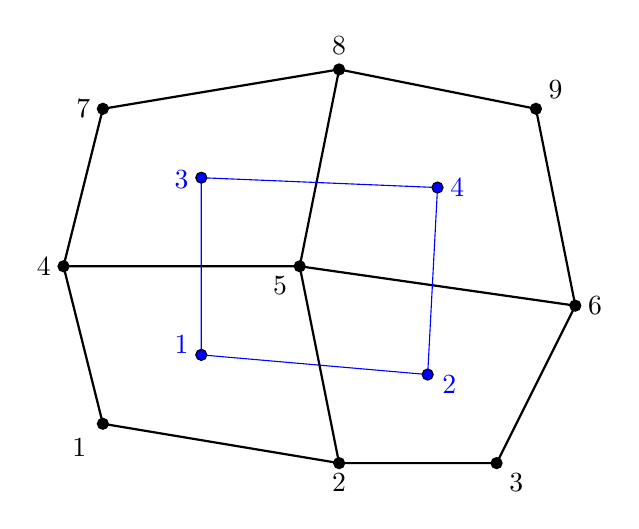
\begin{tikzpicture}
%\draw[fill=gray!5,gray!5](0,0) rectangle (9,7);
%\draw[step=0.5cm,gray,very thin] (0,0) grid (9,7); %background grid
\draw[thick](1.5,1.5) -- (4.5,1) -- (6.5,1) -- (7.5,3) -- (7,5.5) -- (4.5,6) --(1.5,5.5) -- (1,3.5) -- cycle;  
\draw[thick](4.5,1)--(4,3.5)--(4.5,6);
\draw[thick](1,3.5)--(4,3.5)--(7.5,3);

\draw[black,fill=blue] (2.75,2.375) circle (2pt); 
\node[] at (2.5,2.5) {\color{blue}1};
\draw[black,fill=blue] (5.625,2.125) circle (2pt); 
\node[] at (5.9,2) {\color{blue}2};
\draw[black,fill=blue] (5.75,4.5) circle (2pt); 
\node[] at (2.5,4.6) {\color{blue}3};
\draw[black,fill=blue] (2.75,4.625) circle (2pt); 
\node[] at (6,4.5) {\color{blue}4};

\draw[black,fill=black] (1.5,1.5) circle (2pt); \node[] at (1.2,1.2){1}; %1
\draw[black,fill=black] (4.5,1)   circle (2pt); \node[] at (4.5,0.75){2}; %2
\draw[black,fill=black] (6.5,1)   circle (2pt); \node[] at (6.75,0.75){3}; %3
\draw[black,fill=black] (1,3.5)   circle (2pt); \node[] at (0.75,3.5){4}; %4
\draw[black,fill=black] (4,3.5)   circle (2pt); \node[] at (3.75,3.25){5}; %5
\draw[black,fill=black] (7.5,3)   circle (2pt); \node[] at (7.75,3){6}; %6
\draw[black,fill=black] (1.5,5.5) circle (2pt); \node[] at (1.25,5.5){7}; %7
\draw[black,fill=black] (4.5,6)   circle (2pt); \node[] at (4.5,6.3){8}; %8
\draw[black,fill=black] (7,5.5)   circle (2pt); \node[] at (7.25,5.75){9}; %9

\draw[blue](2.75,2.375)--(5.625,2.125)--(5.75,4.5)--(2.75,4.625)--cycle;
\end{tikzpicture}
\end{center}




The values at the corners are $p_1$,
$p_2$, $p_3$ and $p_4$. Assuming that the pressure inside this element can be represented 
by a bilinear field, we have 
\[
p(x,y)= a+ bx +cy +dxy
\]
where the coefficients will be determined by ensuring that $p(x_i,y_i)=p_i$ for $i=1,2,3,4$, or:
\begin{eqnarray}
a+bx_1+cy_1+dx_1y_1 &=& p_1 \\
a+bx_2+cy_2+dx_2y_2 &=& p_2 \\
a+bx_3+cy_3+dx_3y_3 &=& p_3 \\
a+bx_4+cy_4+dx_4y_4 &=& p_4 
\end{eqnarray}
i.e.
\[
\left(
\begin{array}{cccc}
1 & x_1 & y_1 & x_1y_1 \\
1 & x_2 & y_2 & x_2y_2 \\
1 & x_3 & y_3 & x_3y_3 \\
1 & x_4 & y_4 & x_4y_4
\end{array}
\right)\cdot
\left(
\begin{array}{c}
a \\b\\c\\d
\end{array}
\right)
=
\left(
\begin{array}{c}
p_1\\p_2\\p_3\\p_4
\end{array}
\right)
\]

There remains an issue with nodes which are on the boundaries of the domain. These are of course not 
'surrounded' by four pressure values so the above algorithm does not apply directly. However, looking 
at the above figure, and assuming that node 1 is a lower left corner of a 2D domain, we can use the 
bilinear interpolation based on elements 1,2,3,4 to extrapolate a nodal pressure value at node 1. 
The same would apply for nodes 2 and 4 for example. 

\begin{remark}
This scheme is not applicable to quadtree-based meshed.
\end{remark}





\newpage %-----------------------------------------------------------------------------------------
\subsection{Pressure scaling} \index{general}{pressure scaling}
\begin{flushright} {\tiny {\color{gray} pressure\_scaling.tex}} \end{flushright}
%~~~~~~~~~~~~~~~~~~~~~~~~~~~~~~~~~~~~~~~~~~~~~~~~~~~~~~~~~~~~~~~~~~~~~~~~~~~~~~~~~~~~~~~~~~~~~~~~~~

As nicely explained in the 
step 32 of deal.ii\footnote{\url{https://www.dealii.org/9.0.0/doxygen/deal.II/step\_32.html}},
we often need to scale the $\G$ block since it is many orders of magnitude smaller than $\K$ (especially in geodynamics where viscosities are $\sim 10^{22}$), 
which introduces large inaccuracies in the solving process to the point that the solution is nonsensical. 
This scaling coefficient is $\eta/L$ where $\eta$ and $L$ are representative viscosities and lengths. 
We start from 
\[
\left(
\begin{array}{cc}
\K & \G \\ \G^T & -\C 
\end{array}
\right)
\cdot
\left(
\begin{array}{c}
\vec{\cal V} \\ \vec{\cal P}
\end{array}
\right)
=
\left(
\begin{array}{c}
\vec{f} \\ \vec{h}
\end{array}
\right)
\]
and introduce the scaling coefficient as follows (which in fact does not alter the solution at all):
\[
\left(
\begin{array}{cc}
\K & \frac{\eta}{L}\G \\ \frac{\eta}{L}\G^T & - \frac{\eta^2}{L^2} \C 
\end{array}
\right)
\cdot
\left(
\begin{array}{c}
\vec{\cal V} \\\frac{L}{\eta} \vec{\cal P}
\end{array}
\right)
=
\left(
\begin{array}{c}
 \vec{f} \\ \frac{\eta}{L} \vec{h}
\end{array}
\right)
\]
We then end up with the modified Stokes system:
\[
\left(
\begin{array}{cc}
\K & \underline{\G} \\ \underline{\G}^T & \underline{\C} 
\end{array}
\right)
\cdot
\left(
\begin{array}{c}
\vec{\cal V} \\ \underline{\vec{\cal P}}
\end{array}
\right)
=
\left(
\begin{array}{c}
\vec{f} \\ \underline{\vec{h}}
\end{array}
\right)
\]
where 
\[
\underline{\G}=\frac{\eta}{L}\G
\quad\quad
\quad\quad
\underline{\vec{\cal P}}=\frac{L}{\eta} \vec{\cal P}
\quad\quad
\quad\quad
\underline{\C}=\frac{\eta^2}{L^2} \C
\quad\quad
\quad\quad
\underline{\vec{h}}=\frac{\eta}{L}\vec{h}
\]
After the solve phase, we recover the real pressure with $\vec{\cal P}=\frac{\eta}{L}\underline{\vec{\cal P}}$.

Note that in Section~\ref{sec:block_scaling} we revisit the topic and this time 
scale all the blocks of the Stokes matrix.



 %-------------------------------------------
\newpage %-----------------------------------------------------------------------------------------
\subsection{Pressure normalisation, nullspace\label{ss_pnorm}} 
%..................................................
\subsubsection{Basic idea and naive implementation}

When Dirichlet boundary conditions are imposed everywhere on the boundary, pressure is only present by its gradient in 
the equations. It is thus determined up to an arbitrary constant (one speaks then of a null space of size 1).  
In such a case, one commonly impose the average of the pressure over the whole domain or on a subsect of the boundary 
to be have a zero average, i.e.
\[
\int_\Omega p dV = 0
\]
Another possibility is to impose the pressure value at a single node. 

Let us assume that we are using $Q_1 \times P_0$ elements. Then the pressure is constant 
inside each element. 
The integral above becomes:
\[
\int_\Omega p dV = 
\sum_e  \int_{\Omega_e} p dV = 
\sum_e  p_e \int_{\Omega_e} dV = 
\sum_e  p_e A_e = 0
\]
where the sum runs over all elements $e$ of area $A_e$.
This can be rewritten 
\[
\LLL^T \cdot \vec{\cal P}=0
\] 
and it is a constraint on the pressure solution. 
As we have seen before \ref{XXX}, we can associate to it a 
Lagrange multiplier $\lambda$ so that we must solve the modified Stokes system:
\[
\left(
\begin{array}{ccc}
\K & \G & 0\\ 
\G^T & 0 & \LLL \\
0 & \LLL^T & 0
\end{array}
\right)
\cdot
\left(
\begin{array}{c}
\vec{\cal V} \\ \vec{\cal P} \\ \lambda
\end{array}
\right)
=
\left(
\begin{array}{c}
\vec{f} \\ \vec{h} \\ 0
\end{array}
\right)
\]
When higher order spaces are used for pressure (continuous or discontinuous)
one must then carry out the above integration numerically by means of (usually)
a Gauss-Legendre quadrature.

Although valid, this approach has one main disadvantage: it makes the Stokes matrix larger (although
marginally so -- only one row and column are added), but more importantly it prevents the use of some
of the solving strategies of Section \ref{solvers}.


%..................................................
\subsubsection{Implementation -- the real deal}

The idea is actually quite simple and requires two steps:
\begin{enumerate}
\item remove the null space by prescribing the pressure at one location and solve the system;
\item post-process the pressure so as to arrive at a pressure field which fulfills the required normalisation (surface, volume, ...)
\end{enumerate}

\todo[inline]{finish explain}






 %----
\newpage %-----------------------------------------------------------------------------------------
\subsection{Solving the Stokes system \label{sec:solvers}} \begin{flushright} {\tiny {\color{gray} \tt solvers.tex}} \end{flushright}
%~~~~~~~~~~~~~~~~~~~~~~~~~~~~~~~~~~~~~~~~~~~~~~~~~~~~~~~~~~~~~~~~~~~~~~~~~~~~~~~~~~~~~~~~~~~~~~~~~~

Let us start again from the (full) Stokes system:
\begin{equation}
\underbrace{
\left(
\begin{array}{cc}
\K & \G \\ \G^T & -\C 
\end{array}
\right)
}_{\cal A}
\cdot
\left(
\begin{array}{c}
\vec{\cal V} \\ \vec{\cal P}
\end{array}
\right)
=
\left(
\begin{array}{c}
\vec{f} \\ \vec{h}
\end{array}
\right)
\label{StokesSyst}
\end{equation}
We need to solve this system in order to obtain the solution, i.e. the $\vec{\cal V}$ 
and $\vec{\cal P}$ vectors. But how? 
Unfortunately, this question is not simple to answer and the appropriate method depends on many 
parameters, but mainly on how big the matrix blocks are and what the condition number of the matrix $\K$ is. 

First let us start with an obvious question: couldn't we just compute the inverse of the matrix ${\cal A}$?
Under the assumption that the inverse of $\K$ and $\SSS$ exists, we can and we find\footnote{The matrix 
$\C$ is here omitted but it bears no consequences on the conclusion.}
\[
{\cal A}^{-1} = 
\left(
\begin{array}{cc}
\K & \G \\ \G^T & 0
\end{array}
\right)^{-1}
=
\left(
\begin{array}{cc}
\K^{-1} + \K^{-1} \cdot \G \cdot\SSS^{-1} \cdot\G^T \cdot\K^{-1} & -\K^{-1} \cdot\G \cdot\SSS^{-1} \\ 
-\SSS^{-1} \cdot\G^T \cdot\K^{-1}  &  \SSS^{-1}
\end{array}
\right)
\]
However, such an expression is of limited interest in the numerical solution of saddle
point problems since it showcases 5 times the inverse of $\K$ and more importantly
the inverse of the Schur complement matrix $\SSS$ which is likely to be a full matrix so 
that we never want to compute it explicitely.


As concisely explained in Clevenger \& Heister (2021) \cite{clhe21}, 
there are three common approaches used in the literature for solving the above equation on large scales:
\begin{itemize}
\item a pressure corrected, Schur complement CG scheme, using multigrid as an 
approximation to the velocity block;
\item a block-preconditioned Krylov
method, also using multigrid on the velocity block.
For this method, there are two main types:
\begin{itemize}
\item GMRES\cite{mabl15,rumi15} (or any Krylov method not requiring symmetry) with
block-triangular preconditioner (This is what \aspect does):
\[
{\bm P} = \left(
\begin{array}{cc}
\K & \G \\
0 & - \SSS
\end{array}
\right)
\]

\item MINRES\cite{gmhj16} with block-diagonal preconditioner
\[
{\bm P} = \left(
\begin{array}{cc}
\K & 0 \\
0 & - \SSS
\end{array}
\right)
\]

\end{itemize}

\item an all-at-once multigrid performed on the entire Stokes system, using Uzawa-type smoothers.
\end{itemize}



\Literature: Preconditioners for Incompressible Navier-Stokes Solvers 
\begin{small}
\begin{itemize}
\item \fullcite{benz02}
\item \fullcite{bewa08}
\item \fullcite{urvs08}
\item \fullcite{seuv10}
\item Saddle point preconditioners have been extensively discussed and studied \cite{bewa08}, \cite{dewu04}
\item Diagonal preconditioners in \cite{shrb01}, \cite{babc94}.
\end{itemize}
\end{small}

\Literature: Solving Stokes Saddle Point problem
\begin{small}
\begin{itemize}
\item \fullcite{laqu86}
\item \fullcite{rotf90}
\item \fullcite{frha93}
\item \fullcite{elgo94}
\item \fullcite{cheb96}, \fullcite{elma96}
\item \fullcite{brpv97}
\item \fullcite{lixu01}
\item \fullcite{dogs06}, \fullcite{lica06}
\item \fullcite{hoow17}
\item Pragmatic solvers for 3D Stokes problems with heterogeneous coefficients \cite{samb20}
\end{itemize}
\end{small}



%------------------------------------------------------------------------------
\subsection{Block diagonal scaling} \label{sec:block_scaling}

We have already seen in Section~\ref{pscaling} how and why we scale the $\G$ block. 
We revisit this topic more thoroughly in what follows.
This section is borrowed from Section~2.6 of \textcite{mamo08} (2008).

Let us state again the equation we wish to solve (Eq. 6 in the paper):
\[
\begin{pmatrix}
\K & \G \\
\G^T & 0
\end{pmatrix}
\cdot
\begin{pmatrix}
\vec{\cal V} \\
\vec{\cal P}
\end{pmatrix}
=
\begin{pmatrix}
\vec{f} \\
\vec{h}
\end{pmatrix}
\]

Prior to solving this equation, the autors apply a row/column scaling to the equation
to effectively normalize the operators $\K$ and $\G$ with the intention of
reducing round off errors. The scaling is particularly important for
problems in geodynamics when dimensional quantities are used to
define the problem and because of the large, local variations which
may occur in the constitutive tensor (in practice, the effective viscosity) . 

They apply a symmetric block diagonal scaling to the equation via the scaling matrix\footnote{
The $S$ stands for 'scaling', the Schur complement is given by $\SSS$}
\[
{\bm S} = 
\begin{pmatrix}
{\bm S}_1 & 0 \\ 0 & {\bm S}_2
\end{pmatrix}
\]
Writing the first equation as ${\bm A} \cdot \vec{x} = \vec{b}$, 
the symmetric scaling operation is applied as follows:
\[
{\bm S}^{-1} \cdot {\bm A} \cdot \vec{x}= {\bm S}^{-1} \cdot \vec{b} 
\]
followed by\footnote{${\bm S}^{-T}$ is the inverse of the transpose of the matrix.} 
\[
{\bm S}^{-1} \cdot {\bm A} \cdot {\bm S}^{-T} \cdot {\bm S}^T \cdot \vec{x}= {\bm S}^{-1} \cdot \vec{b} 
\]
to give the scaled system ${\bm A}_s \cdot \vec{y}_s = \vec{b}_s$ , where the operator 
${\bm A}_s$ is given by
\begin{eqnarray}
{\bm S}^{-1} \cdot {\bm A} \cdot {\bm S}^{-T} 
&=&\begin{pmatrix}
{\bm S}_1^{-1} & 0 \\ 0 & {\bm S}_2^{-1}
\end{pmatrix}
\cdot 
\begin{pmatrix}
\K & \G \\
\G^T & 0
\end{pmatrix}
\cdot
\begin{pmatrix}
{\bm S}_1^{-T} & 0 \\ 0 & {\bm S}_2^{-T}
\end{pmatrix} \nn\\
&=&
\begin{pmatrix}
{\bm S}_1^{-1} \cdot \K \cdot {\bm S}_1^{-T} & {\bm S}_1^{-1} \cdot \G \cdot {\bm S}_2^{-T} \\
({\bm S}_1^{-1} \cdot \G \cdot {\bm S}_2^{-T})^{T} & 0 
\end{pmatrix} \nn\\
&=&
\begin{pmatrix}
\K_s & \G_s \\
\G^T_s & 0
\end{pmatrix} \nn\\
&=&{\bm A}_s \nn
\end{eqnarray}
with
\[
{\bm S}^T \cdot \vec{x} 
= 
\begin{pmatrix}
{\bm S}_1^T \cdot \vec{\cal V} \\
{\bm S}_2^T \cdot \vec{\cal P}
\end{pmatrix}
=\vec{y}_s
\qquad\qquad
{\bm S}^{-1} \cdot \vec{b} = 
\begin{pmatrix}
{\bm S}_1^{-1}\cdot\vec{f} \\
{\bm S}_2^{-1}\cdot\vec{h}
\end{pmatrix}
=\vec{b}_s
\]
Following the solution of the scaled system, we recover the un-scaled
solution from $\vec{x} = {\bm S}^{-T} \cdot  \vec{y}_s$. 
The form of the scaling operation is based
on the preconditioner described in Rusten and Winther (1992). For
the purpose of scaling, rather than full preconditioning of the indefinite system, 
we let both ${\bm S}_1$ and ${\bm S}_2$ be diagonal matrices. We seek
to approximately normalize the operators $\K$ and $\G$.

Thus we let 
\[
S_1(i,i) = \sqrt{ \max_j K_{ij}} \qquad \forall i \in [1,NfemV]
\]
The choice for ${\bm S}_2$ is based on the requirement that $\G^T_s\cdot \G_s \simeq {\bm 1}_{Nfemp}$ (i.e.
the identity matrix of size $NfemP\times NfemP$) which yields the relation
\[
\G^T_s \cdot \G = ({\bm S}_1^{-1} \cdot \G \cdot {\bm S}_2^{-T})^T 
\cdot ({\bm S}_1^{-1} \cdot \G \cdot {\bm S}_2^{-T} )
= {\bm S}_2^{-1} \cdot \G^T \cdot {\bm S}_1^{-T} \cdot {\bm S}_1^{-1} \cdot \G \cdot {\bm S}_2^{-T} = {\bm 1}
\]
We can left multiply by ${\bm S}_2$ and right multiply by  ${\bm S}_2^T$ to obtain
\[
\G^T \cdot {\bm S}_1^{-T} \cdot {\bm S}_1^{-1} \cdot \G = {\bm S}_2 \cdot {\bm S}_2^T
\]
We can approximately satisfy this equation if we first define the vector $\vec{g}$ of size $NfemV$
\[
g_i = \max_j(G_{ij}) 
\]
and then let
\[
S_2(i,i)=\frac{1}{NfemV} \sqrt{ \left( \sum_k S_1^2(k,k) \right)   \vec{g}_i \cdot \vec{g}_i}
\]
Note that in the paper the above equation (their eq.37) does not contain any $i$ in the rhs, 
which is probably missing from the $\vec{g}$ vectors.


{\color{red} sent email to Dave May 15/01/2026}



%...................................................
\subsection{When using the penalty formulation}

In this case we are only solving for velocity since pressure has been eliminated 
and is later recovered in a post-processing step. The linear system is of the form:
\[
(\K_\eta+\K_\lambda) \cdot \vec {\cal V} = \vec f
\]
 We also know that 
the penalty factor $\lambda$ is many orders of magnitude higher than the viscosity and 
in combination with the use of the $Q_1 \times P_0$ element the resulting matrix 
condition number is very high so that the use of iterative solvers is precluded. 
Indeed codes such as \sopale \cite{full95}, \douar \cite{brtf08}, \fantom \cite{thie11} 
or \sulec \cite{qube11} relying on the penalty formulation all use direct solvers.
The most popular are BLKFCT\footnote{\url{http://dm.unife.it/blkfclt/}}, 
MUMPS\footnote{\url{http://mumps.enseeiht.fr/}}\cite{amdu89,amdl00,amdk01,amgl06,ambl19}, 
PasTiX \cite{herr02},
WSMP\footnote{\url{http://www.research.ibm.com/projects/wsmp}} \cite{GUPTA94ieee,GUPTA09sc-long},
UMFPACK and CHOLMOD\footnote{\url{http://faculty.cse.tamu.edu/davis/suitesparse.html}}
, SuperLU\footnote{\url{https://portal.nersc.gov/project/sparse/superlu/}}, 
PARDISO\footnote{\url{https://www.pardiso-project.org/}}
\cite{pardiso-6.0a,pardiso-6.0b,pardiso-6.0c}, or those inside 
PETSc\footnote{\url{https://www.mcs.anl.gov/petsc/}}.

Braun \etal (2008) \cite{brtf08} list the following features of direct solvers:
\begin{itemize}
\item Robust
\item Black-box operation
\item Difficult to parallelize
\item Memory consumption
\item Limited scalability
\end{itemize}

The main advantage of direct solvers is used in this case: They can solve ill-conditioned 
matrices. However, memory requirements for the storage of number of nonzeros in the 
Cholesky matrix grow very fast as the number of equations/grid size increases, especially in 3D,
to the point that even modern computers with tens of Gb of RAM cannot deal with a $\sim 100^3$ element mesh.
This explains why direct solvers are often used for 2D problems and rarely in 3D with noticeable 
exceptions \cite{thfb08,yahb09,brya10,lobh10,alht11,alht12,alhf13,whbb14,neew18}. 

Note that \textcite{pedr24} (2024) conducted a detailed study comapring 
MUMPS, UMFPACK, and Intel DSS (PARDISO).
The conclusions are 
\begin{displayquote}
{\color{darkgray}
1. Intel DSS is not ready for production codes because it computes incorrect results without warnings;\\
2. UMFPACK reaches the memory limit earlier than the other solvers and must be configured with the automatic
symmetry strategy to yield correct results; and\\
3. MUMPS is not thread-safe and, in particular, does not work well with OpenBLAS, which causes thread 'locks' and
conflicts. However, MUMPS works well with Intel MKL and is the only solver able to tackle massive systems.}
\end{displayquote}
In \textcite{saramito} we find the following table whigh gives the aymptotic computing time versus the 
size of the sparse matrix $n$ and the geometry dimension $d$:
\[
\begin{array}{lcc}
d& \text{factorize} & \text{solve} \\
\hline\hline
1& n & n \\
2& n^{3/2} & n \log n \\
3& n^2 & n^{4/3}\\
\hline
\end{array}
\]

%....................................................................
\subsection{Uzawa algorithms and the Schur complement approach }

\index{general}{Uzawa algorithm}

Let us write the above system as two equations:
\begin{eqnarray}
\K \cdot \vec{\cal V} + \G \cdot \vec{\cal P} &=& \vec{f} \nn\\
\G^T \cdot  \vec{\cal V} - \C \cdot \vec{\cal P} &=& \vec{h} \nn
\end{eqnarray}
Again, $\C$ is typically non-zero in the case of stabilised elements or if a 
penalty formulation is used. 
The first line can be re-written 
$\vec{\cal V}=\K^{-1}\cdot (\vec{f} - \G \cdot \vec{\cal P})$ and can be inserted in the second:
\begin{equation}
\G^T\cdot \vec{\cal V} =\G^T \cdot  [ \K^{-1} \cdot  (\vec{f} - \G \cdot  \vec{\cal P}) ] - \C\cdot \vec{\cal P} = \vec{h} 
\end{equation}
which can be written: 
\begin{mdframed}[backgroundcolor=blue!5]
\begin{equation}
(\G^T \cdot \K^{-1} \cdot \G + \C) \cdot \vec{\cal P} = \G^T \cdot \K^{-1}\cdot \vec{f} - \vec{h} 
\end{equation}
\end{mdframed}
The matrix $\SSS= \G^T \cdot \K^{-1} \cdot \G + \C$ is called the Schur complement. 
\index{general}{Schur Complement} 
It is Symmetric (since $\K$ is symmetric) and  Positive-Definite\footnote{$M$ 
positive definite $\iff$ $x^TMx>0$ $\forall \; x\in \mathbb{R}^n \setminus {\bm 0}$ }
(SPD) \index{general}{SPD} if $Ker({\G})=0$. 
Having solved this equation (i.e. we have obtained $\vec{\cal P}$), the velocity can be recovered by solving 
$\K\cdot \vec{\cal V} =\vec{f}- \G \cdot \vec{\cal P}$. 

\begin{remark}
The Schur complement matrix naturally occurs when the Stokes matrix is decomposed using 
a LDU block-factorisation. Indeed, we have 
\[
\left(
\begin{array}{cc}
\K & \G \\ 
\G^T & 0
\end{array}
\right)
=
\left(
\begin{array}{cc}
{\bm I} & 0 \\ 
\G^T \cdot \K^{-1} & {\bm I}
\end{array}
\right)
\cdot
\left(
\begin{array}{cc}
\K & 0 \\ 
0 & -\SSS
\end{array}
\right)
\cdot
\left(
\begin{array}{cc}
{\bm I} & \K^{-1} \cdot \G \\ 
0 & {\bm I}
\end{array}
\right)
\]
\end{remark}

For now, let us assume that we have built the $\SSS$ matrix\footnote{We will 
revisit this topic later on, but be aware that we never build $\SSS$ in practice.} 
and the right hand 
side $\underline{\vec{f}}=\G^T \cdot \K^{-1} \cdot \vec{f} - \vec{h}$.
We must then solve $\SSS\cdot \vec{\cal P} = \underline{\vec{f}}$.
It is easy to see that $\SSS$ is actually a full matrix (i.e. not sparse) and 
aside from the costs of building it, explicitly using a direct solver would require 
a lot (i.e. too much in practice) of memory so that we must then turn to iterative methods. 

\index{general}{Richardson Iterations}
One can resort to so-called Richardson iterations, defined as follows 
(e.g., see Varga \cite{varga}, p141):
in solving the matrix equation ${\bm A}\cdot {\vec X}={\vec b}$,
the Richardson iterative method is defined by: 
\begin{equation}
{\vec X}_{k+1} = {\vec X}_k + \alpha_k (-{\bm A} \cdot {\vec X}_k + {\vec b})
\quad\quad
m\geq 0 
\end{equation}
where the $\alpha_k$'s are real scalars. 
It is easy to see that when the method converges then ${\vec X}_{k+1} \simeq {\vec X}_k$  and then 
for $\alpha_k\neq 0$ then ${\bm A}\cdot {\vec X}={\vec b}$ is satisfied. 
In our case, it writes:
\begin{eqnarray}
\vec {\cal P}_{k+1} 
&=& \vec {\cal P}_{k} + \alpha_k ( - \SSS \cdot \vec{\cal P}_{k}  +  \underline{\vec{f}}) \nonumber\\
&=& \vec {\cal P}_{k} + \alpha_k \left[ - (\G^T \cdot \K^{-1} \cdot \G + \C)  \cdot \vec{\cal P}_{k} 
+  (\G^T \cdot \K^{-1} \cdot \vec{f} - \vec{h}   ) \right] \nonumber\\
&=& \vec {\cal P}_{k} + \alpha_k \left[ \G^T \cdot \K^{-1} \cdot ( - \G \cdot \vec{\cal P}_{k} + \vec{f}) 
-\C \cdot \vec{\cal P}_{k} - \vec{h} 
\right] \nonumber\\
&=& \vec {\cal P}_{k} + \alpha_k \left[ \G^T \cdot \K^{-1} \cdot ( \K\cdot \vec{\cal V}_k)
-\C \cdot \vec{\cal P}_{k}  - \vec{h} \right] \nonumber\\
&=& \vec {\cal P}_{k} + \alpha_k \left( \G^T \cdot \vec{\cal V}_k -\C \cdot \vec{\cal P}_{k} - \vec{h} \right) 
\end{eqnarray}
The above iterations are then carried out and for each new pressure field the associated velocity field 
is computed. The method of using Richardson iterations applied to the Schur complement 
is commonly called the Uzawa algorithm (see Braess \cite[p221]{braess}
\footnote{I have slightly 
altered the indices of the velocities wrt the book}).

\begin{mdframed}[backgroundcolor=blue!5]
\underline{\bf Uzawa algorithm (1)}: assume $\vec{\cal P}_0$ known
\begin{eqnarray}
\text{solve} \qquad \mathbb{K} \cdot \vec{\cal V}_k &=& \vec f - \mathbb{G}\cdot \vec {\cal P}_{k} \\
\vec{\cal P}_{k+1} &=& 
\vec{\cal P}_{k}  + \alpha_k (\mathbb{G}^T\cdot \vec{\cal V}_k  -\C \cdot \vec{\cal P}_{k} -\vec h)
\quad
\quad
\quad
\quad
k=0,1,2, ... \label{uzaa2}
\end{eqnarray}
\end{mdframed}
This same algorithm is to be found on page 59 of \cite{saramito}.

This method is rather simple to implement, although
what makes an appropriate set of $\alpha_k$ values is not 
straightforward, which is why the conjugate gradient method (or any method
which computes an optimal $\alpha_k$ in some sense) is often preferred, 
as detailed in the next section. 

It is known that such iterations will converge for $0< \alpha < \rho(\SSS)= \lambda_{max}(\SSS)$ 
where $\rho(\SSS)$ is the spectral radius of the matrix $\SSS$
which is essentially the largest, in absolute value, eigenvalue of $\SSS$ (neither of which 
can be computed easily).  
It can also be proven that the rate of convergence depends on the condition number of the matrix.

Richardson iterations are part of the family of stationary iterative 
methods\footnote{\url{https://mathworld.wolfram.com/StationaryIterativeMethod.html}}, 
since it can be rewritten 
\begin{equation}
{\vec X}_{k+1} = ({\bm I} - \alpha_k {\bm A} ) \cdot {\vec X}_k + \alpha_k {\vec b}
\end{equation}
which is the definition of a stationary method. 
The four main stationary methods are the Jacobi method, 
Gauss-Seidel method, successive overrelaxation method (SOR), 
and symmetric successive overrelaxation method (SSOR).
\index{general}{Jacobi Iterative Method}
\index{general}{Gauss-Seidel Iterative Method}
\index{general}{SOR Iterative Method}
\index{general}{SSOR Iterative Method}

Since the $\alpha$ parameter is the key to a successful Uzawa algorithm, 
this issue has of course been investigated. What follows is 
presented in p221 of Braess \cite{braess}.
For the analysis of the Uzawa algorithm, we define the residual
\[
\vec {\cal R}_k = \vec h - \mathbb{G}^T \cdot \vec{\cal V}_k  +\C \cdot \vec{\cal P}_{k}
\]
In addition, suppose the solution of the saddle point problem is denoted
by $(\vec{\cal V}^\star,\vec{\cal P}^\star)$ so that we have
\[
\vec{f} = \K \cdot \vec{\cal V}^\star + \G \cdot \vec{\cal P}^\star
\qquad
{\rm and}
\qquad
\vec{h} = \G^T \cdot \vec{\cal V}^\star - \C \cdot \vec{\cal P}^\star 
\]

Now substituting the iteration formula for ${\cal V}_k$, and inserting $\vec{f}$ and $\vec{h}$ from above,
we get
\begin{eqnarray}
\vec{\cal R}_k 
&=& \vec{h} -\G^T  \cdot \vec{\cal V}_k  +\C \cdot \vec{\cal P}_{k} \nn\\
&=& \vec{h} -\mathbb{G}^T\cdot \mathbb{K}^{-1} (\vec f - \mathbb{G}\cdot \vec{\cal P}_{k})  +\C \cdot \vec{\cal P}_{k}\nn\\
&=& (\G^T\cdot\vec{\cal V}^\star - \C \cdot \vec{\cal P}^\star) -\mathbb{G}^T\cdot \mathbb{K}^{-1} (\K\cdot\vec{\cal V}^\star 
+ \G\cdot\vec{\cal P}^\star - {\G}\cdot \vec{\cal P}_{k})+\C \cdot \vec{\cal P}_{k} \nn\\
&=& ({\G}^T \cdot \mathbb{K}^{-1} \cdot \mathbb{G} + \C)\cdot (\vec {\cal P}_{k} - \vec{\cal P}^\star) 
\end{eqnarray}
From Eq.~\eqref{uzaa2} it follows that:
\begin{eqnarray}
\vec{\cal P}_{k+1} - \vec{\cal P}_{k}  
&=& \alpha\; (\mathbb{G}^T\cdot \vec{\cal V}_k -\C \cdot \vec{\cal P}_{k} -\vec h) \\
&=& -\alpha\; \vec{\cal R}_k \\ 
&=& -\alpha\; ( \mathbb{G}^T \cdot \mathbb{K}^{-1} \cdot \mathbb{G} + \C )
\cdot (\vec {\cal P}_{k} -\vec{\cal P}^\star)\\ 
&=& \alpha\; (\mathbb{G}^T \cdot \mathbb{K}^{-1} \cdot \mathbb{G} + \C) \cdot 
(\vec{\cal P}^\star - \vec {\cal P}_{k} ) 
\end{eqnarray}
Thus the Uzawa algorithm is equivalent to applying the gradient method 
to the reduced equation using a fixed step size. 
In particular, the iteration converges for
$
\alpha < 2 || \G^T \cdot \K^{-1} \cdot \G + \C||^{-1}
$
and one can show that the good step size $\alpha_k$ is given by\footnote{I need to include matrix $\C$.}
\begin{equation}
\alpha_k = \frac{\vec{\cal R}_k \cdot \vec{\cal R}_k}
{(\G \cdot \vec{\cal R}_k)\cdot (\K^{-1}\cdot \G \cdot \vec{\cal R}_k)}
\label{uzaa3}
\end{equation}



However, if we were to use this rule formally, we would 
need an additional multiplication by $\K^{-1}$ in every step 
of the iteration. This can be avoided by storing an 
auxiliary vector. 
Note that this algorithm is presented in Zienkiewicz \etal (1985) \cite{zivt85} 
in the context of viscoplastic flow.

%Note that in \cite{glow} it is stated: the convergence of this algorithm is proved for 
%$\alpha \in (0,2\mu/d)$ (where $d$ is the number of dimensions).
%\todo[inline]{check this, and report page number}

As mentioned above, there is a way to rework the original Uzawa algorithm 
to include Eq. (\ref{uzaa3}). It is yields a modified 
Uzawa algorithm (see p222 of Braess \cite{braess}
\footnote{I have slightly 
altered the indices of the velocities wrt the book}):


\begin{mdframed}[backgroundcolor=blue!5]
\underline{\bf Uzawa algorithm (2)}: assume $\vec{\cal P}_0$ known. 
Solve $\mathbb{K}\cdot \vec{\cal V}_0 = \vec f - \mathbb{G}\cdot  \vec{\cal P}_0$. 
For $k=0,1,2,...$, compute 
\begin{eqnarray}
\vec{\cal R}_k=\vec q_k &=& \vec h-\mathbb{G}^T \cdot \vec{\cal V}_k + \C \cdot \vec{\cal P}_{k}\\
\vec{p}_k &=& {\G}\cdot q_k \\
\vec H_k &=& {\K}^{-1}\cdot \vec{p}_k \\
\alpha_k &=& \frac{\vec q_k \cdot \vec q_k}{\vec{p}_k \cdot \vec H_k} \\
\vec {\cal P}_k &=& \vec {\cal P}_{k-1} - \alpha_k  \vec q_k \\
\vec {\cal V}_{k} &=& \vec {\cal V}_{k-1} + \alpha_k  \vec H_k
\end{eqnarray}
\end{mdframed}


\Literature: \\
\begin{itemize}
\item
\fullcite{cach88}
\item
\fullcite{bamn02}
\item
\fullcite{cao03}
\item
\fullcite{kosa11}
\end{itemize}

These Uzawa methods have been implemented in \stone~147.


\newpage
%...................................................
\subsection{Conjugate gradient and the Schur complement approach }
\label{ss:schurpcg}

\index{general}{CG} \index{general}{Conjugate Gradient}
Since the Schur matrix $\SSS$ is Symmetric Positive Definite, 
the Conjugate Gradient (CG) 
method\footnote{\url{https://en.wikipedia.org/wiki/Conjugate_gradient_method}} \cite{hest52} 
is very appropriate to solve this system. 

Indeed, looking at the definition of Wikipedia: "{\it In mathematics, the conjugate 
gradient method is an algorithm for the numerical solution of particular systems of 
linear equations, namely those whose matrix is symmetric and positive-definite. 
The conjugate gradient method is often implemented as an iterative algorithm, applicable 
to sparse systems that are too large to be handled by a direct implementation or other 
direct methods such as the Cholesky decomposition. 
Large sparse systems often arise when numerically solving partial differential 
equations or optimization problems.}"

See also the excellent document by J. Shewchuk entitled {\it 
An Introduction to the Conjugate Gradient Method Without the Agonizing Pain}
available at \url{https://www.cs.cmu.edu/~quake-papers/painless-conjugate-gradient.pdf}.

A simple Wikipedia search (crossed-checked against other online sources) 
tells us that the Conjugate Gradient algorithm is as follows:

\vspace{0.4cm}

\begin{minipage}{0.48\textwidth}
\centering
{\captionfont Algorithm as obtained from Wikipedia.}\\
\frame{\includegraphics[width=8cm]{images/solvers/cgwiki}}
\end{minipage}\hfill
\begin{minipage}{0.48\textwidth}
\centering
{\captionfont Algorithm as obtained from Shewchuck}\\
\frame{\includegraphics[width=8cm]{images/solvers/shewchuk.png}}
\end{minipage}

\vspace{.5cm}

The same algorithm with our notations (we wish to solve $\SSS\cdot \vec{\cal P}=\underline{\vec{f}}$):
\begin{itemize}
\item $\vec{r}_0 = \underline{\vec{f}} - \SSS \cdot \vec{\cal P}_0$
\item $\vec{p}_0 = \vec{r}_0$
\item $k=0$ 
\item repeat
\begin{itemize}
\item $\alpha_k = (\vec{r}_k^T\cdot \vec{r}_k )/(\vec{p}_k^T \cdot \SSS\cdot  \vec{p}_k )$
\item $\vec{\cal P}_{k+1} = \vec{\cal P}_k+\alpha_k \vec{p}_k$
\item $\vec{r}_{k+1} = \vec{r}_k - \alpha_k \; \SSS \cdot \vec{p}_k $ 
\item if $\vec{r}_{k+1}$ is sufficiently small, exit loop.
\item $\beta_k=(\vec{r}_{k+1}^T \cdot \vec{r}_{k+1})/(\vec{r}_k^T \cdot \vec{r}_k)$ 
\item $\vec{p}_{k+1} =\vec{r}_{k+1}+ \beta_k \vec{p}_k$ 
\item $k=k+1$ 
\end{itemize}
\item return $\vec{\cal P}_{k+1}$ as the result
\end{itemize}

This algorithm is of course explained in detail in many textbooks such as Saad \cite{saad},
in Zhong, Yuen, Moresi \& Knepley (2012) \cite{zhym12}, and in Section~\ref{ss:itsolvers}.

Let us look at this algorithm more closely. The parts which may prove to be somewhat tricky 
are those involving the matrix the Schur complement matrix since we wish never to build 
it explicitely. We start the iterations with a guess pressure $\vec{\cal P}_0$ (and an initial guess velocity 
which is obtained by solving $\K\cdot \vec{\cal V}_0 =\vec{f}- \G\cdot \vec{\cal P}_0$).
\begin{eqnarray}
\vec{r}_0 
&=& \underline{\vec{f}}-\SSS \cdot \vec{\cal P}_0 \nn\\
&=& \G^T\cdot \K^{-1}\cdot \vec{f} - \vec{h} - (\G^T\cdot \K^{-1}\cdot \G + \C)\cdot \vec{\cal P}_0 \nn\\ 
&=& \G^T\cdot \K^{-1}\cdot (\vec{f} - \G\cdot \vec{\cal P}_0) - \vec{h} \nn\\
&=& \G^T\cdot \K^{-1}\cdot \K\cdot \vec{\cal V}_0 -\C \cdot \vec{\cal P}_0 - \vec{h} \nn\\ 
&=& \G^T\cdot \vec{\cal V}_0  -\C \cdot \vec{\cal P}_0   - \vec{h}  
\end{eqnarray}
We see that we were able to compute $\SSS \cdot \vec{\cal P}_0$ without ever forming the 
Schur complement matrix explicitely. We now turn to the $\alpha_k$ coefficient:
\[
\alpha_k 
= \frac{\vec{r}_k^T\cdot \vec{r}_k }{\vec{p}_k \cdot \SSS\cdot  \vec{p}_k } 
= \frac{\vec{r}_k^T \cdot \vec{r}_k }{\vec{p}_k\cdot (\G^T \cdot \K^{-1} \cdot \G +\C )\cdot \vec{p}_k } 
= \frac{\vec{r}_k^T \cdot \vec{r}_k }{(\G\cdot \vec{p}_k)^T \cdot  \K^{-1} \cdot (\G \cdot \vec{p}_k) + \vec{p}_k\cdot \C\cdot \vec{p}_k } 
\]
We then define $\tilde{\vec{p}}_k = \G \cdot \vec{p}_k$, so that $\alpha_k$ can be computed as follows:
\begin{enumerate}
\item compute $\tilde{\vec{p}}_k = \G \cdot  \vec{p}_k$
\item solve $\K\cdot  \vec{d}_k = \tilde{\vec{p}}_k$
\item compute 
\[
\alpha_k=\frac{\vec{r}_k^T \cdot \vec{r}_k}{\tilde{\vec{p}}_k^T \cdot \vec{d}_k 
+ \vec{p}_k^T \cdot \C\cdot \vec{p}_k }
\]
\end{enumerate}
Then we need to look at the term $\SSS\cdot \vec{p}_k$:
\[
\SSS\cdot \vec{p}_k = (\G^T\cdot \K^{-1}\cdot \G\cdot +\C )\vec{p}_k 
= \G^T\cdot \K^{-1}\cdot \tilde{\vec{p}}_k  + \C\cdot \vec{p}_k= \G^T\cdot  \vec{d}_k + \C \cdot \vec{p}_k
\]
We can then rewrite the CG algorithm as follows: 
\begin{itemize}
\item choose $\vec{\cal P}_0$
\item compute $\vec{\cal V}_0$ solution of $\K\cdot \vec{\cal V}_0 =\vec{f}- \G\cdot \vec{\cal P}_0$ 
\item $\vec{r}_0 = \G^T\cdot \vec{\cal V}_0 - \C \cdot \vec{\cal P}_0 - \vec{h}$ 
\item if $\vec{r}_0$ is sufficiently small, then return $(\vec{\cal V}_0,\vec{\cal P}_0)$ as the result
\item $\vec{p}_0=\vec{r}_0$
\item $k=0$
\item repeat
\begin{itemize}
\item compute $\tilde{\vec{p}}_k = \G\cdot \vec{p}_k$
\item solve $\K\cdot  \vec{d}_k = \tilde{\vec{p}}_k$
\item compute $\alpha_k=(\vec{r}_k^T \cdot  \vec{r}_k)/
              (\tilde{\vec{p}}_k^T\cdot \vec{d}_k + \vec{p}_k^T\cdot \C\cdot\vec{p}_k)$
\item $\vec{\cal P}_{k+1} = \vec{\cal P}_k+\alpha_k \vec{p}_k$
\item $\vec{r}_{k+1} = \vec{r}_k - \alpha_k (\G^T \cdot \vec{d}_k + \C \cdot \vec{p}_k) $
\item if $\vec{r}_{k+1}$ is sufficiently small, then exit loop
\item $\beta_k=(\vec{r}_{k+1}^T \cdot \vec{r}_{k+1})/(\vec{r}_k^T \cdot \vec{r}_k)$
\item $\vec{p}_{k+1} =\vec{r}_{k+1}+ \beta_k \vec{p}_k$
\item $k=k+1$
\end{itemize}
\item return $\vec{\cal P}_{k+1}$ as result
\end{itemize}
We see that we have managed to solve the Schur complement equation with the Conjugate Gradient method
without ever building the matrix $\SSS$. Having obtained the pressure solution $\vec{\cal P}_{k+1}$, 
we can easily recover 
the corresponding velocity with $\K\cdot \vec{\cal V}_{k+1} =\vec{f}- \G\cdot \vec{\cal P}_{k+1}$. 
However, this is rather unfortunate because it requires yet another solve with the $\K$ matrix. 
As it turns out, we can slightly alter the above algorithm to have it update the velocity 
as well so that this last solve is unnecessary.

We have 
\begin{eqnarray}
\vec{\cal V}_{k+1} 
&=& \K^{-1}\cdot (f - \G\cdot \vec{\cal P}_{p+1} ) \nn\\
&=& \K^{-1}\cdot (f - \G\cdot (\vec{\cal P}_k+\alpha_k \vec{p}_k) ) \nn\\
&=& \K^{-1}\cdot (f - \G\cdot \vec{\cal P}_k) - \alpha_k \K^{-1}\cdot \G \cdot \vec{p}_k \nn\\
&=& \vec{\cal V}_k - \alpha_k \K^{-1}\cdot \tilde{\vec{p}}_k  \nn\\
&=& \vec{\cal V}_k - \alpha_k \vec{d}_k 
\end{eqnarray}
and we can insert this simple and cheap calculation inside the algorithm and get the velocity solution 
nearly for free. The final Conjugate Gradient algorithm is then 

\newpage
\begin{mdframed}[backgroundcolor=blue!5]
\underline{\bf solver\_cg}: assume $\vec{\cal P}_0$ known
\begin{itemize}
\item compute $\vec{\cal V}_0=\K^{-1}\cdot (\vec{f}-\G \cdot \vec{\cal P}_0)$
\item $\vec{r}_0 = \G^T\cdot \vec{\cal V}_0 -\C \cdot \vec{\cal P}_0 - \vec{h}$ 
\item if $\vec{r}_0$ is sufficiently small, then return $(\vec{\cal V}_0,\vec{\cal P}_0)$ as the result
\item $\vec{p}_0=\vec{r}_0$
\item $k=0$
\item repeat
\begin{itemize}
\item compute $\tilde{\vec{p}}_k = \G \cdot \vec{p}_k$
\item solve $\K\cdot \vec{d}_k = \tilde{p}_k$
\item compute $\alpha_k=(\vec{r}_k^T \cdot  \vec{r}_k)/(\tilde{\vec{p}}_k^T \cdot \vec{d}_k 
      + \vec{p}_k^T \cdot \C\cdot \vec{p}_k)$
\item $\vec{\cal P}_{k+1} = \vec{\cal P}_k+\alpha_k \vec{p}_k$
\item $ \vec{\cal V}_{k+1} = \vec{\cal V}_k - \alpha_k \vec{d}_k$
\item $\vec{r}_{k+1} = \vec{r}_k - \alpha_k (\G^T \cdot \vec{d}_k + \C \cdot \vec{p}_k) $
\item if $\vec{r}_{k+1}$ is sufficiently small ($||\vec{r}_{k+1}||_2/||\vec{r}_0||_2 <tol$), then exit loop
\item $\beta_k=(\vec{r}_{k+1}^T \cdot \vec{r}_{k+1})/(\vec{r}_k^T \cdot \vec{r}_k)$
\item $\vec{p}_{k+1} =\vec{r}_{k+1}+ \beta_k \vec{p}_k$
\item $k=k+1$
\end{itemize}
\item return $\vec{\cal P}_{k+1}$ as result
\end{itemize}
\end{mdframed}

\begin{remark}
Again, the matrix $\C$ is rarely present unless for example when stabilised elements are used 
such as the stabilised $Q_1\times P_0$ or the stabilised $Q_1\times Q_1$ elements.
\end{remark}

This iterative algorithm will converge to the solution with a rate which depends on 
the condition number of the $\SSS$ matrix, which is not easy to compute since 
$\SSS$ is never built. However, it has been established that large viscosity contrasts in the domain 
will have a negative impact on the convergence. 

\begin{remark} 
This algorithm requires one solve with matrix $\K$ per iteration 
but says nothing about the method employed to do so (direct or iterative solver)
nor the corresponding preconditioner.
\end{remark} 

\index{general}{Preconditioned Conjugate Gradient}  
One thing we know improves the convergence of any iterative solver is the use of a 
preconditioner matrix and therefore now focus on the Preconditioned Conjugate Gradient (PCG) method.
Once again we turn to Wikipedia\footnote{\url{https://en.wikipedia.org/wiki/Conjugate_gradient_method}}:
and read: ``In most cases, preconditioning is necessary to ensure 
fast convergence of the conjugate gradient method. If ${\bm M}^{-1}$ is 
symmetric positive-definite and ${\bm M}^{-1}\cdot {\bm A}$ has a better condition number than 
${\bm A}$, a preconditioned conjugate gradient method can be used. It takes the following form:''

\begin{minipage}{0.43\textwidth}
\centering
{\captionfont Algorithm as obtained from Wikipedia.}\\
\frame{\includegraphics[width=7cm]{images/solvers/pcgwiki}}
\end{minipage}\hfill
\begin{minipage}{0.52\textwidth}
\begin{center}
{\captionfont Algorithm as found in Saad \cite{saad}}\\
\frame{\includegraphics[width=9cm]{images/solvers/saad}}
\end{center}
\end{minipage}

\vspace{0.5cm}


The same algorithm with our notations:
\begin{itemize}
\item $\vec{r}_0 = \underline{\vec{f}} - \SSS \cdot \vec{\cal P}_0$ 
\item $\vec{z}_0= {\bm M}^{-1} \cdot \vec{r}_0$ 
\item $\vec{p}_0 = \vec{z}_0$
\item $k=0$ 
\item repeat
\begin{itemize}
\item $\alpha_k = (\vec{r}_k^T\cdot \vec{z}_k )/(\vec{p}_k^T \cdot \SSS\cdot  \vec{p}_k )$
\item $\vec{\cal P}_{k+1} = \vec{\cal P}_k+\alpha_k \vec{p}_k$
\item $\vec{r}_{k+1} = \vec{r}_k - \alpha_k \; \SSS \cdot \vec{p}_k $ 
\item $\vec{z}_{k+1} = {\bm M}^{-1} \cdot \vec{r}_{k+1}$ 
\item $\beta_k=(\vec{z}_{k+1}^T \cdot \vec{r}_{k+1})/(\vec{z}_k^T \cdot \vec{r}_k)$ 
\item $\vec{p}_{k+1} =\vec{z}_{k+1}+ \beta_k \vec{p}_k$ 
\item $k=k+1$ 
\end{itemize}
\item return $\vec{\cal P}_{k+1}$ as the result
\end{itemize}



Note that in the algorithm above the preconditioner matrix ${\bm M}$ 
has to be symmetric positive-definite and fixed, i.e., cannot change from iteration to iteration. 
We see that this algorithm introduces an additional vector $\vec{z}$ and a solve with the 
matrix ${\bm M}$ at each iteration, which means that ${\bm M}$ must 
be such that solving ${\bm M}\cdot \vec{x}= \vec{f}$ 
where $\vec{f}$ is a given rhs vector must be cheap. Ultimately, the PCG algorithm applied to 
the Schur complement equation takes the form:

\newpage
\begin{mdframed}[backgroundcolor=blue!5]
\underline{\bf solver\_pcg}: assume $\vec{\cal P}_0$ known
\begin{itemize}
\item compute $\vec{\cal V}_0=\K^{-1}(\vec{f}-\G\cdot \vec{\cal P}_0)$
\item $\vec{r}_0 = \G^T \cdot \vec{\cal V}_0 - \C \cdot \vec{\cal P}_0 - \vec{h}$
\item if $\vec{r}_0$ is sufficiently small, then return $(\vec{\cal V}_0,\vec{\cal P}_0)$ as the result
\item $\vec{z}_0= M^{-1} \cdot \vec{r}_0$ 
\item $\vec{p}_0=\vec{z}_0$
\item $k=0$
\item repeat
\begin{itemize}
\item compute $\tilde{\vec{p}}_k = \G \cdot \vec{p}_k$
\item solve $\K\cdot  \vec{d}_k = \tilde{\vec{p}}_k$
\item compute $\alpha_k=(\vec{r}_k^T \cdot \vec{z}_k)/(\tilde{\vec{p}}_k^T \cdot \vec{d}_k
      + \vec{p}_k^T\cdot\C \cdot \vec{p}_k$)
\item $\vec{\cal P}_{k+1} = {\cal P}_k+\alpha_k \vec{p}_k$
\item $\vec{\cal V}_{k+1} = {\cal V}_k - \alpha_k \vec{d}_k$
\item $\vec{r}_{k+1} = \vec{r}_k - \alpha_k (\G^T \cdot \vec{d}_k + \C \cdot \vec{p}_k) $
\item if $\vec{r}_{k+1}$ is sufficiently small (i.e. $||\vec{r}_{k+1}||_2/||\vec{r}_0||_2 <tol$), 
      then exit loop
\item $\vec{z}_{k+1}=M^{-1} \cdot \vec{r}_{k+1}$
\item $\beta_k=(\vec{z}_{k+1}^T \cdot  \vec{r}_{k+1})/(\vec{z}_k^T \cdot  \vec{r}_k)$
\item $\vec{p}_{k+1} =\vec{z}_{k+1}+ \beta_k \vec{p}_k$
\item $k=k+1$
\end{itemize}
\item return $\vec{\cal P}_{k+1}$ as result
\end{itemize}
\end{mdframed}

Preconditioners of the Schur complement matrix are discussed in Section~\ref{sec:precond_S}







\newpage
%......................................................
\subsection{Generalized Conjugate Residual approach (Geenen \etal (2009))}

This approach is presented in \textcite{geum09} (2009).  
The saddle point problem arising from the constrained Stokes equation is 
solved with a Krylov method, GCR \cite{vavu94}, right preconditioned (postconditioned) 
with a block triangular preconditioner (BTR) \cite{brpa88}.

The preconditioner ${\bm P}$ is given by
\[
{\bm P} = \left(
\begin{array}{cc}
\K & \G \\
0 & - \tilde{\SSS}
\end{array}
\right)
\]

The GCR algorithm \cite{eies83} in this case is taken from Vuik \etal (2000) \cite{vusb00}
and makes use of the block triangular preconditioner as follows:
\begin{itemize}
\item[] $\vec{r}_0 = \vec{b} - {\bm A}\cdot \vec{x}^0$
\item[] for $k$=0,1,2,...
\begin{itemize}
\item $\vec{s}^{k+1}={\bm P}^{-1} \cdot \vec{r}^k$
\item $\vec{v}^{k+1} = {\bm A}\cdot \vec{s}^{k+1}$
\item for i=0,1,...$k$
\begin{itemize}
\item $\vec{v}^{k+1}=\vec{v}^{k+1} - (\vec{v}^{k+1},\vec{v}^{i}) \vec{v}^i$
\item $\vec{s}^{k+1}=\vec{s}^{k+1} - (\vec{v}^{k+1},\vec{v}^{i}) \vec{s}^i$
\end{itemize}
\item end for
\item $\vec{v}^{k+1}=\vec{v}^{k+1} / \| \vec{v}^{k+1} \|_2$
\item $\vec{s}^{k+1}=\vec{s}^{k+1} / \| \vec{v}^{k+1} \|_2$  
\item $\vec{x}^{k+1} = \vec{x}^k + (\vec{v}^{k+1},\vec{r}^k) \vec{s}^{k+1} $
\item $\vec{r}^{k+1} = \vec{r}^k - (\vec{v}^{k+1}, \vec{r}^k) \vec{v}^{k+1}$
\end{itemize}
\item[] end for
\end{itemize}

As explained in Geenen \etal, instead of constructing ${\bm P}^{-1}$
explicitely and applying it to $\vec{r}$, we instead solve the system 
${\bm P}\cdot \vec{s} = \vec{r}$. We first decompose $\vec{r}$ and $\vec{s}$
as follows:
\[
\vec{r}^k = \left( \begin{array}{c} \vec{r}_\upnu^k \\ \vec{r}_p^k   \end{array} \right)
\qquad
\vec{s}^{k+1} = \left( \begin{array}{c} \vec{s}_\upnu^{k+1} \\ \vec{s}_p^{k+1}   \end{array} \right)
\]
so that we have to solve 
\[
\left(
\begin{array}{cc}
\K & \G \\
0 & - \tilde{\SSS}
\end{array}
\right)
\cdot
\left( \begin{array}{c} \vec{s}_\upnu^{k+1} \\ \vec{s}_p^{k+1}   \end{array} \right)
=
\left( \begin{array}{c} \vec{r}_\upnu^k \\ \vec{r}_p^k   \end{array} \right)
\]
This is actually rather trivial because of the upper triangular nature of the preconditioner ${\bm P}$.
It immediately follows:
\begin{eqnarray}
\tilde{\SSS}\cdot  \vec{s}_p^{k+1} &=& -\vec{r}_p^k   \\
\K \cdot \vec{s}_\upnu^{k+1} &=& \vec{r}_\upnu^k - \G \cdot \vec{s}_p^{k+1}
\end{eqnarray}
As before we now must specify how we solve the above two equations (and we must therefore
make a choice about the approximate Schur complement $\tilde{\SSS}$).

In the paper they take ${\bm  M}_p$, the pressure mass matrix scaled with the inverse of viscosity 
as an approximation to the Schur complement $\tilde{\SSS}$, which is spectrally equivalent.
Note that sometimes this mass matrix can be lumped which makes solving with it trivial and fast.

The inner solve with $\K$ is carried out with a CG solvers preconditioned with AMG. They 
state that ``Using AMG as a preconditioner to CG for the subsystem solution
guarantees $h$-independent convergence of the solver during the preconditioner construction phase.''


%......................................................
\subsection{The Arrow-Hurwicz algorithm}

This is borrowed from algorithm 8.7 in \textcite{saad}.

\begin{itemize}
\item[] Select an initial guess $\vec{\cal V}^0$ and $\vec{\cal P}^0$ 
\item[] for $k$=0,1,2,... until convergence
\begin{itemize}
\item $\vec{\cal V}^{k+1}=\vec{\cal V}^k + \epsilon ( \vec{f}- \K \cdot \vec{\cal V}^k - \G \cdot \vec{\cal P}^k )$
\item $\vec{\cal P}^{k+1}=\vec{\cal P}^k + \omega ( \G^T \cdot \vec{\cal V}^{k+1} - \vec{h})$
\end{itemize}
\end{itemize}

The above algorithm is a block-iteration of the form
\[
\left(
\begin{array}{cc}
I & 0 \\
-\omega \G^T & I
\end{array}
\right)
\cdot
\left(
\begin{array}{c}
\vec{\cal V}^{k+1} \\
\vec{\cal P}^{k+1}
\end{array}
\right)
=
\left(
\begin{array}{cc}
I-\epsilon \K & -\epsilon \G \\
0 & I
\end{array}
\right)
\cdot
\left(
\begin{array}{c}
\vec{\cal V}^{k} \\
\vec{\cal P}^{k}
\end{array}
\right)
+
\left(
\begin{array}{c}
\epsilon \vec{f} \\
-\omega \vec{h}
\end{array}
\right)
\]



%......................................................
\subsection{Using MINRES a la Burstedde \etal (2008)}

This approach is presented in Burstedde \etal (2008) \cite{bugg08}.
They state that neglecting the off-diagonal blocks motivates use of the symmetric
positive definite preconditioner:
\[
{\bm P} = \left(
\begin{array}{cc}
\tilde{\K} & 0 \\
0 & \tilde{\SSS}
\end{array}
\right)
\]
where $\tilde{\K}$ is a variable-viscosity discrete vector Laplacian
approximation of $\K$ (see explanations in \cite{bugs09}), 
which is motivated by the fact that
for constant viscosity and Dirichlet boundary conditions,
$\K$ and $\tilde\K$ are equivalent. 
$\tilde{\SSS}$ is an approximation of
the Schur complement given by a lumped mass matrix
weighted by the inverse viscosity $\eta^{-1}$. The resulting
diagonal matrix $\tilde{\SSS}$ is spectrally equivalent to $\SSS$ \cite{elsw}.
They also use AMG as preconditioner for the inner solves. 

Note that Burstedde \etal  (2008) \cite{bugg08} relies on stabilised 
$Q_1\times Q_1$ elements from Dohrmann \& Bochev \cite{dobo04} 
so that their Stokes matrix does feature the associated $-\C$ block.
Subsequent papers do so too, see Burstedde \etal (2009) \cite{bugs09}, 
Burstedde \etal (2013) \cite{busa13}.
The same solver structure based on MINRES is used in these articles too.

%---------------------------------------------
\subsection{The Augmented Lagrangian approach}
\index{general}{Augmented Lagrangian}


We start from the saddle point Stokes system:
\begin{equation}
\left(
\begin{array}{cc}
\K & \G \\ \G^T & 0 
\end{array}
\right)
\cdot
\left(
\begin{array}{c}
\vec{\cal V} \\ \vec{\cal P}
\end{array}
\right)
=
\left(
\begin{array}{c}
\vec{f} \\ \vec{h}
\end{array}
\right)
\label{StokesSyst2}
\end{equation}
The AL method consists of subtracting $\lambda^{-1} \mathbb{M}_p \cdot \vec{\cal P}$ from the left and 
right-side of the mass conservation equation (where $\mathbb{M}_p$ is the pressure mass matrix) 
and introducing the following iterative scheme:
\begin{equation}
\left(
\begin{array}{cc}
\K & \G \\ \G^T & -\lambda^{-1} \mathbb{M}_p
\end{array}
\right)
\cdot
\left(
\begin{array}{c}
\vec{\cal V}^{k+1} \\ \vec{\cal P}^{k+1}
\end{array}
\right)
=
\left(
\begin{array}{c}
\vec{f} \\ \vec{h} - \lambda^{-1} \mathbb{M}_p \cdot \vec{\cal P}^k
\end{array}
\right)
\label{ALStokes}
\end{equation}
where $k$ is the iteration counter and $\lambda$ is an artificial compressibility term which has 
the dimensions of dynamic viscosity. 
The choice of $\lambda$ can be difficult as too low or too high a value yields either erroneous results and/or terribly ill-conditioned matrices. The LaCoDe paper \cite{demh19} uses such a method and report 
that $\lambda=\max_\Omega({\eta})$ works well. 
Note that at convergence we have $||\vec{\cal P}^{k+1}-\vec{\cal P}^k||<\epsilon$ and then Eq.(\ref{ALStokes}) converges to Eq.(\ref{StokesSyst2}) and the velocity and pressure fields are solution of the unmodified system Eq.(\ref{StokesSyst2}).

The introduction of this term serves one purpose: allowing us to solve the system 
in a segregated manner (i.e. computing successive iterates of the velocity and pressure 
fields until convergence is reached). The second line of Eq.~(\ref{ALStokes}) is 
\[
\G^T \cdot \vec{\cal V}^{k+1} - \lambda^{-1} \mathbb{M}_p \cdot \vec{\cal P}^{k+1} = \vec{h} - \lambda^{-1} \mathbb{M}_p \cdot \vec{\cal P}^k
\]
and can therefore be rewritten
\[
\vec{\cal P}^{k+1} = \vec{\cal P}^k + \lambda \mathbb{M}_p^{-1} \cdot (\G^T \cdot \vec{\cal V}^{k+1} - \vec h)
\]
We can then substitute this expression of $\vec{\cal P}^{k+1}$ in the first equation. This yields:
\begin{eqnarray}
\K \cdot \vec{\cal V}^{k+1}  
&=& \vec f - \G \cdot {\cal P}^{k+1}) \\
\K \cdot \vec{\cal V}^{k+1}  
&=& \vec f - \G \cdot ( \vec{\cal P}^k + \lambda \mathbb{M}_p^{-1} \cdot  (\G^T \cdot \vec{\cal V}^{k+1} - \vec h)  ) \\
\K \cdot \vec{\cal V}^{k+1} + \lambda \G \cdot \mathbb{M}_p^{-1} \cdot \G^T \cdot \vec{\cal V}^{k+1} 
&=& \vec f - \G \cdot ( \vec{\cal P}^k - \lambda \mathbb{M}_p^{-1}\vec h)  ) \\
\underbrace{  \left(  \K  + \lambda \G \cdot \mathbb{M}_p^{-1} \cdot \G^T \right)   }_{\tilde{\K}  } \cdot \vec{\cal V}^{k+1} 
&=& \underbrace{ \vec f - \G \cdot ( \vec{\cal P}^k - \lambda \mathbb{M}_p^{-1}\vec h)  )}_{\vec{f}^{k+1}} \\
\end{eqnarray}
The iterative algorithm goes as follows:
\begin{mdframed}[backgroundcolor=blue!5]
\begin{enumerate}
\item if it is the first timestep, set $\vec{\cal P}^0=0$ , otherwise set it to the pressure of the previous timestep.
\item calculate $\tilde{\K}$
\item calculate $\vec{f}^{k+1}$
\item solve $\tilde{\K} \cdot \vec{\cal V}^{k+1} = \vec{f}^{k+1}$
\item update pressure with 
$\vec{\cal P}^{k+1} = \vec{\cal P}^k + \lambda \mathbb{M}_p^{-1} \cdot (\G^T \cdot \vec{\cal V}^{k+1} - \vec h)$
\end{enumerate}
\end{mdframed}

\begin{remark} 
If discontinuous pressures are used, the pressure mass matrix can be inverted element by element which is 
cheaper than inverting $\M_p$ as a whole. If the pressure field is continuous computing the inverse 
of the pressure mass matrix is definitely not a viable option.
\end{remark}

\begin{remark} 
This method has obvious ties with the penalty method. 
\end{remark}

\begin{remark} 
If $\lambda >> \max_\Omega(\eta)$ then the matrix $\tilde{\K}$ is ill-conditioned and 
a direct solver must probably be used.
\end{remark}

\newpage
%------------------------------------------------------------------------------
\subsection{The SIMPLE method}
\index{general}{SIMPLE} 
\begin{flushright} {\tiny {\color{gray} simple.tex}} \end{flushright}
%~~~~~~~~~~~~~~~~~~~~~~~~~~~~~~~~~~~~~~~~~~~~~~~~~~~~~~~~~~~~~~~~~~~~~~~~~~~~~~~~~~~~~~~~~~~~~~~~~~


What follows is borrowed from \fullcite{john16}, page 666. 

The SIMPLE method (Semi-Implicit Method for Pressure-Linked Equations)
has been introduced by \textcite{pasp72} (1972) as an iterative method to solve
the finite volume discretized incompressible Navier-Stokes equations. 

The algorithm is based on the following steps (adapted from \cite{eche13}):
\begin{itemize}
\item First the pressure is assumed to be known from the previous iteration.
\item Then the velocity is solved from the momentum equations. The newly obtained
velocities do not satisfy the continuity equation since the pressure is only a
guess.
\item In the next substeps the velocities and pressures are corrected in order to
satisfy the discrete continuity equation.
\end{itemize}

SIMPLE relies on the block LU decomposition
\begin{equation}
\left(\begin{array}{cc}
\K & \G \\ \G^T & 0  
\end{array}\right)
\cdot
\left(\begin{array}{c}
\vec{\cal V} \\ \vec{\cal P}
\end{array}\right)
=
\left(\begin{array}{cc}
\K & 0 \\ \G^T & -\SSS
\end{array}\right)
\cdot
\left(\begin{array}{cc}
{\bm I} & \K^{-1} \cdot \G \\
0 & {\bm I} 
\end{array}\right)
\cdot
\left(\begin{array}{c}
\vec{\cal V} \\ \vec{\cal P}
\end{array}\right)
=
\left(\begin{array}{c}
\vec{f} \\ \vec{h}
\end{array}\right)
\end{equation}

The approximation $\K^{-1}$ as ${\bm D}_\K^{-1} = (\text{diag}(\K))^{-1}$ leads to the 
SIMPLE algorithm. In this case the approximation of the Schur complement matrix is given by
$\tilde{\SSS} = \G^T\cdot  {\bm D}_\K^{-1} \cdot \G$  and the decomposition looks like
\[
\left(
\begin{array}{cc}
\K & \G \\ \G^T & -\C 
\end{array}
\right)
\simeq
\left(
\begin{array}{cc}
\K & 0 \\ 
\G^T & -\tilde{\SSS}
\end{array}
\right)
\cdot
\left(
\begin{array}{cc}
{\bm I} & {\bm D}_\K^{-1} \cdot \G \\
0 & {\bm I} 
\end{array}
\right)
\]
Thus one iteration of SIMPLE solves the following system:
\[
\left(
\begin{array}{cc}
\K & \G \\ \G^T & -\C 
\end{array}
\right)
\simeq
\left(
\begin{array}{cc}
\K & 0 \\ 
\G^T & -\tilde{\SSS}
\end{array}
\right)
\cdot
\left(
\begin{array}{cc}
{\bm I} & {\bm D}_\K^{-1} \cdot \G \\
0 & {\bm I} 
\end{array}
\right)
\cdot
\left(
\begin{array}{c}
\vec{\cal V} \\ \vec{\cal P}
\end{array}
\right)
=
\left(
\begin{array}{c}
\vec{f} \\ \vec{h}
\end{array}
\right)
\]

Before we can write out the SIMPLE algorithm, we must first take a small detour via so-called
distributive iterative methods \cite{vusb00,tack10}. 
Let us consider the linear system 
\[
{\bm A}\cdot \vec{x}=\vec{b}
\] 
A stationary iterative method is defined as follows:
\[
\vec{x}^{k+1}= {\bm B}\cdot \vec{x}^{k}+ \vec{c}
\]
where $\vec{c}=({\bm I}-{\bm B})\cdot {\bm A}^{-1}\cdot \vec{b}$. 
Left-multiplying all terms by $({\bm I}-{\bm B})^{-1}$ first and then left-multiplying again 
by ${\bm A}$  we arrive at:
\[
{\bm A}\cdot ({\bm I}-{\bm B})^{-1}\cdot \vec{x}^{k+1}
={\bm A}\cdot ({\bm I}-{\bm B})^{-1}\cdot {\bm B}\cdot 
\vec{x}^{k} + {\bm A}\cdot ({\bm I}-{\bm B})^{-1} \cdot \vec{c}
\]
We define ${\bm M}={\bm A}\cdot ({\bm I}-{\bm B})^{-1} $ so that now
\[
{\bm M}\cdot\vec{x}^{k+1}={\bm M}\cdot {\bm B}\cdot \vec{x}^{k}+\vec{b} 
\]
We define ${\bm N}={\bm M}\cdot {\bm B}$
and finally 
\[
{\bm M}\cdot\vec{x}^{k+1}={\bm N}\cdot \vec{x}^{k}+\vec{b} 
\]
Note that ${\bm M}-{\bm N}={\bm M}-{\bm M}\cdot {\bm B}
= {\bm M}\cdot  ({\bm I}-{\bm B}) 
= {\bm A}\cdot ({\bm I}-{\bm B})^{-1}\cdot ({\bm I}-{\bm B}) 
= {\bm A}$. 
Let us now write the original system 
${\bm A}\cdot \vec{x}=\vec{b}$ as $({\bm A}\cdot {\bm B})\cdot ({\bm B}^{-1}\cdot \vec{x})=\vec{b}$
or, $ \underline{\bm A}\cdot  \underline{\vec{x}}=\vec{b} $
with 
$\vec{x}={\bm B}\cdot \underline{\vec{x}}$
and 
$\underline{\bm A}={\bm A}\cdot {\bm B}$.
Splitting $\underline{\bm A}={\bm M}-{\bm N}$ again yields 
\[
{\bm M}\cdot \underline{\vec{x}}^{k+1}={\bm N}\cdot \underline{\vec{x}}^{k}+\vec{b} 
\]
Using $\vec{x}={\bm B}\cdot \underline{\vec{x}}$, we get 
\[
{\bm M}\cdot {\bm B}^{-1}\cdot \vec{x}^{k+1} = {\bm N}\cdot {\bm B}^{-1}\cdot  \vec{x}^{k}+\vec{b} 
\]
We can then 'solve' for $\vec{x}^{k+1}$ and we then have 
\begin{eqnarray}
\vec{x}^{k+1}
&=&  {\bm B}\cdot {\bm M}^{-1} \cdot[ {\bm N} \cdot  {\bm B}^{-1}  \cdot \vec{x}^{k}+ \vec{b}  ] \nn\\
&=&  {\bm B}\cdot {\bm M}^{-1} \cdot[ ({\bm M} - \underline{\bm A}) \cdot  {\bm B}^{-1}\cdot \vec{x}^{k}+\vec{b}  ]\nn\\
&=&  {\bm B}\cdot {\bm M}^{-1} \cdot[ ({\bm M} - {\bm A}\cdot {\bm B}) \cdot  {\bm B}^{-1}\cdot  \vec{x}^{k}+ \vec{b}  ]\nn\\
&=&  {\bm B}\cdot {\bm M}^{-1} \cdot[ {\bm M}\cdot {\bm B}^{-1} \cdot \vec{x}^{k} - {\bm A}\cdot {\bm B}\cdot  {\bm B}^{-1} \cdot \vec{x}^{k}+\vec{b}  ]\nn\\
&=&  {\bm B}\cdot {\bm M}^{-1} \cdot[ {\bm M}\cdot {\bm B}^{-1} \cdot \vec{x}^{k} - {\bm A}\cdot \vec{x}^{k}+ \vec{b}  ]\nn\\
&=&  \vec{x}^k + {\bm B}\cdot {\bm M}^{-1}\cdot [ \vec{b}    - {\bm A} \cdot \vec{x}^{k}  ] \nn
\end{eqnarray}
Finally, we have the following recursion:
\begin{equation}
\boxed{\vec{x}^{k+1} = \vec{x}^k +{\bm B} \cdot {\bm M} ^{-1}\cdot (\vec{b} -{\bm A}\cdot \vec{x}^{k}  ) }
\label{eq:simplerec}
\end{equation}
Coming back to the SIMPLE algorithm, we start from 
\[
{\bm A}=
\left(
\begin{array}{cc}
\K & \G \\
\G^T & 0
\end{array}
\right)
\]
The matrix ${\bm B}$ is then chosen to be 
\[
{\bm B}=
\left(
\begin{array}{cc}
{\bm I} & -\K^{-1} \cdot \G \\
0 & {\bm I}
\end{array}
\right)
\]
We then have 
\[
{\bm A}\cdot  {\bm B} = 
\left(
\begin{array}{cc}
\K & \G \\
\G^T & 0
\end{array}
\right)
\cdot 
\left(
\begin{array}{cc}
{\bm I} & -\K^{-1} \cdot \G \\
0 & {\bm I}
\end{array}
\right)
=
\left(
\begin{array}{cc}
\K & 0 \\
\G^T & -\SSS
\end{array}
\right)
\]
where $\SSS=\G^T \cdot \K^{-1} \cdot \G$.
Let us recall that we define ${\bm D}_\K =\text{diag}(\K)$ and $\hat{\SSS}=\G^T \cdot {\bm D}_\K^{-1} \cdot \G$. 
We further define 
\[
{\bm M}=
\left(
\begin{array}{cc}
\K & 0 \\
\G^T & -\hat{\SSS}
\end{array}
\right)
\]
and ${\bm N}$ follows from the splitting ${\bm A}\cdot {\bm B}= {\bm M} - {\bm N}$. 
(Note that we do not need to form nor use ${\bm N}$).

The standard SIMPLE algorithm also replaces $\K^{-1}$  by  ${\bm D}_\K^{-1}$ in ${\bm B}$ so that 
${\bm B}$ is approximated by:
\[
{\bm B}=
\left(
\begin{array}{cc}
{\bm I} & -{\bm D}_\K^{-1} \cdot \G \\
0 & {\bm I}
\end{array}
\right)
\]
in the iterations.
We can define 
\[
\vec{r}^k=
\vec{b}-{\bm A}\cdot \vec{x}^k = 
\left(
\begin{array}{c}
\vec{f} \\ \vec{h}
\end{array}
\right)
-
\left(
\begin{array}{cc}
\K & \G \\
\G^T & 0
\end{array}
\right)
\cdot
\left(
\begin{array}{c}
\vec{\cal V}^k \\ \vec{\cal P}^k
\end{array}
\right)
=
\left(
\begin{array}{c}
\vec{r}_{\cal V}^k \\ \vec{r}_{\cal P}^k
\end{array}
\right)
\]

The iteration loop of Eq.~\eqref{eq:simplerec} then takes the form 
\[
\left(
\begin{array}{c}
\vec{\cal V}^{k+1} \\ 
\vec{\cal P}^{k+1}
\end{array}
\right)
=
\left(
\begin{array}{c}
\vec{\cal V}^k \\ 
\vec{\cal P}^k
\end{array}
\right)
+ 
{\bm B}\cdot  {\bm M} ^{-1}
\left(
\begin{array}{c}
r_{\cal V}^k \\ r_{\cal P}^k
\end{array}
\right)
=
\left(
\begin{array}{c}
\vec{\cal V}^k \\ 
\vec{\cal P}^k
\end{array}
\right)
+ 
\left(
\begin{array}{c}
\delta \vec{\cal V}^k \\ 
\delta \vec{\cal P}^k
\end{array}
\right)
\quad
\textrm{with}\quad
\left(
\begin{array}{c}
\delta \vec{\cal V}^k \\ 
\delta \vec{\cal P}^k
\end{array}
\right)
=
{\bm B} \cdot {\bm M}^{-1}
\left(
\begin{array}{c}
\vec{r}_{\cal V}^k \\ 
\vec{r}_{\cal P}^k
\end{array}
\right)
\]
This last equation can be rewritten\footnote{Remember 
that $({\bm A}\cdot {\bm B})^{-1}={\bm B}^{-1}\cdot {\bm A}^{-1}$}:
\[
{\bm M} \cdot 
\left[ {\bm B}^{-1} \cdot 
\left(
\begin{array}{c}
\delta \vec{\cal V}^k \\ 
\delta \vec{\cal P}^k
\end{array}
\right)
\right]
=
\left(
\begin{array}{c}
\vec{r}_{\cal V}^k \\ 
\vec{r}_{\cal P}^k
\end{array}
\right)
\]
We then have to solve 
\begin{equation}
{\bm M} 
\cdot
\left(
\begin{array}{c}
\delta^\star \vec{\cal V}^k \\ 
\delta^\star \vec{\cal P}^k
\end{array}
\right)
=
\left(
\begin{array}{cc}
\K & 0 \\
\G^T & -\hat{\SSS}
\end{array}
\right)
\cdot
\left(
\begin{array}{c}
\delta^\star \vec{\cal V}^k \\ 
\delta^\star \vec{\cal P}^k
\end{array}
\right)
=
\left(
\begin{array}{c}
\vec{r}_{\cal V}^k \\ 
\vec{r}_{\cal P}^k
\end{array}
\right)
\label{simple1aa}
\end{equation}
and then compute
\begin{equation}
\left(
\begin{array}{c}
\delta \vec{\cal V}^k \\ 
\delta \vec{\cal P}^k
\end{array}
\right)
=
{\bm B} \cdot 
\left(
\begin{array}{c}
\delta^\star \vec{\cal V}^k \\ 
\delta^\star \vec{\cal P}^k
\end{array}
\right)
\label{simple2aa}
\end{equation}
Fortunately Eq.~\eqref{simple1aa} translates into:
\begin{eqnarray}
\K \cdot \delta^\star \vec{\cal V}^k &=&  \vec{r}_{\cal V}^k   \\
\hat{\SSS} \cdot  \delta^\star \vec{\cal P}^k &=&  - \vec{r}_P^k + \G^T \cdot \delta^\star \vec{\cal V}^k 
\end{eqnarray}
and Eq.~\eqref{simple2aa} translates into:
\[
\left(
\begin{array}{c}
\delta \vec{\cal V}^k \\ 
\delta \vec{\cal P}^k
\end{array}
\right)
=
\left(
\begin{array}{cc}
{\bm I} & -{\bm D}_\K^{-1}\cdot \G \\
0 & {\bm I}
\end{array}
\right)
\cdot
\left(
\begin{array}{c}
\delta^\star \vec{\cal V}^k \\ 
\delta^* \vec{\cal P}^k
\end{array}
\right)
\]
or, 
\begin{eqnarray}
\delta \vec{\cal V}_k &=& \delta^\star \vec{\cal V}^k 
-{\bm D}_\K^{-1}\cdot \G \cdot\delta^\star \vec{\cal P}_k \\
\delta \vec{\cal P}_k &=& \delta^\star \vec{\cal P}^k
\end{eqnarray}


The final algorithm will then look as follows:

\begin{mdframed}[backgroundcolor=blue!5]
\begin{enumerate}
\item compute the residuals 
\begin{eqnarray}
\vec{r}_{\cal V} &=& \vec{f} - \K \cdot \vec{\cal V}^{(k)} - \G \cdot \vec{\cal P}^{(k)} \nn\\
\vec{r}_{\cal P} &=& \vec{h} - \G^T \cdot \vec{\cal V}^{(k)}
\end{eqnarray}
\item Solve $\K  \cdot \delta^\star \vec{\cal V}^k =  \vec{r}_{\cal V}^k  $
\item Solve $\hat{\SSS} \cdot \delta^\star \vec{\cal P}^k =  \vec{r}_{\cal P}^k - \G^T \cdot  \delta^\star \vec{\cal V}^k $
\item Compute $\delta \vec{\cal V}^k = \delta^\star \vec{\cal V}^k -{\bm D}_\K^{-1} \cdot \G \cdot \delta^\star \vec{\cal P}_k $
\item Update $\delta \vec{\cal P}^k = \delta^\star \vec{\cal P}^k$
\item Update 
\begin{eqnarray}
\vec{\cal V}^{(k+1)} &=& \vec{\cal V}^{(k)} + \omega_{\cal V} \; \delta \vec{\cal V}^{(k)} \nn\\
\vec{\cal P}^{(k+1)} &=& \vec{\cal P}^{(k)} + \omega_{\cal P} \; \delta \vec{\cal P}^{(k)} 
\end{eqnarray}
\end{enumerate}
\end{mdframed}
where the parameters $\omega_{\cal V}$ and $\omega_{\cal P}$ are between 0 and 1. 

Note that SIMPLE can be used as left and as right preconditioner, 
see page 669 of \textcite{john16}.

Also, John states that:
``SIMPLE is easily to implement, which makes
it attractive. It relies on the already assembled matrix blocks. Only the approximation 
$\hat{\SSS}$ of the Schur complement matrix has to be computed. This
matrix couples pressure degrees of freedom that are usually not coupled in finite
element approximations of the diffusion operator, but it is still a sparse matrix.
The efficiency of SIMPLE depends on how good $\K^{-1}$ is approximated by its
diagonal.''


Note that SIMPLE is also discussed (and improved?) in \cite{brsa97b} (1997). 


\newpage
What follows is taken from section 6.5.1 of the book by \cite{tack10}.
I have adapted their notations to fit the ones of FieldStone. 
In retrospect this is not as well explained as the material above 
taken from \textcite{john16} but we obtain the same algorithm. 

\subsection*{Distributive iterations}
To apply the method of distributive iterations (Section 6.3.4 of the book), initially we define
\[
\mathbb{A} = \begin{pmatrix}
\K & \G \\
\G^T & 0
\end{pmatrix}
\]
We choose a distribution matrix $\mathbb{B}$ such as to represent 
$\mathbb{A}\cdot \mathbb{B}$ in a block-triangular form:
\begin{equation}
{\mathbb A}\cdot {\mathbb B} = 
\begin{pmatrix}
\mathbb{Q} & 0 \\
\mathbb{R} & \mathbb{T}
\end{pmatrix}
\label{simple:eq1}
\end{equation}
Splitting $\mathbb{A}\cdot \mathbb{B} = \mathbb{M} - \mathbb{L}$\footnote{we find $M-N$ in the book, 
but $N$ is already defined at the 1-1 block of the matrix $A$, so I use $L$ instead.} is easily obtained by splitting $\mathbb{Q}$ and $\mathbb{T}$, 
leading to simple separate updates for velocity and pressure. A possible choice for ${\mathbb B}$ is
\[
{\mathbb B} = 
\begin{pmatrix}
\mathbb{I} & \mathbb{B}_{12} \\
0 &  \mathbb{B}_{22} 
\end{pmatrix}
\]
and hence 
\[
{\mathbb A}\cdot {\mathbb B} = 
\begin{pmatrix}
\K & \K \cdot \mathbb{B}_{12} + \G \cdot \mathbb{B}_{22} \\
\G^T & \G^T \cdot \mathbb{B}_{12}
\end{pmatrix}
\]
Choosing $\mathbb{B}_{12}$ and $\mathbb{B}_{22}$ such that $\K \cdot \mathbb{B}_{12} + \G \cdot \mathbb{B}_{22} =0$ results in the block-triangular form \eqref{simple:eq1}.
Therefore we choose
$\mathbb{B}_{12} = - \K^{-1} \cdot \G \cdot \mathbb{B}_{22} $ which leads to:
\[
{\mathbb A}\cdot {\mathbb B} 
= 
\begin{pmatrix}
\K & 0 \\
\G^T & - \G^T \cdot \K^{-1} \cdot \G \cdot \mathbb{B}_{22} 
\end{pmatrix}
= 
\begin{pmatrix}
\K & 0 \\
\G^T & - \SSS \cdot \mathbb{B}_{22} 
\end{pmatrix}
=
\begin{pmatrix}
\mathbb{Q} & 0 \\
\mathbb{R} & \mathbb{T}
\end{pmatrix}
\]
with $\mathbb{T} = - \SSS \cdot \mathbb{B}_{22}$, $\mathbb{Q}=\K$, $\mathbb{R}=\G^T$ and with $\mathbb{B}_{22}$ still to be chosen.

Various methods result from the choice of $\mathbb{B}_{22}$. We present one of the choices in
the next section, i.e. the SIMPLE method.

\subsection*{The SIMPLE method}

A method widely known in the literature as the SIMPLE method (Semi-Implicit Method for
Pressure-Linked Equations) is proposed in \textcite{pasp72} (1972) and discussed in detail in the book by \textcite{patankar1980} (1980). This is perhaps the oldest and most widely used iterative method
for the Stokes equations. The SIMPLE method is obtained by choosing 
$\mathbb{B}_{22}={\bm 1}$, so that now $\mathbb{T}=\SSS$ and then
\[
{\mathbb A}\cdot {\mathbb B}  
=
\begin{pmatrix}
\K & 0 \\
\G^T & - \SSS
\end{pmatrix}
=
\begin{pmatrix}
\K & 0 \\
\G^T & - \G^T \cdot \K^{-1} \cdot \G 
\end{pmatrix}
\]
where $\SSS$ is the standard Schur complement.
A splitting ${\mathbb A}\cdot {\mathbb B} = \M-\mathbb{L}$ is defined by
\[
\mathbb{M}
=
\begin{pmatrix}
\mathbb{Q} & 0 \\
\G^T & \mathbb{T}
\end{pmatrix}
\]
where $\mathbb{Q}$ is an approximation to $\K$ (which we will
denote by $\hat{\mathbb{K}}$)
and $\mathbb{T}$ is an approximation to $-\SSS$
(which we will denote by $-\hat{\mathbb{S}}$)
such that $\mathbb{M}\cdot \vec{x} = \vec{b}$ is easily solvable.
Then
\[
\mathbb{M}=
\begin{pmatrix}
\hat{\mathbb{K}} & 0 \\
\G^T & -\hat{\mathbb{S}}
\end{pmatrix}
\]
where $\hat{\mathbb{K}}$ and $\hat{\mathbb{S}}$ are approximations to $\K$ 
and $\SSS $ 

For the distribution step in (6.55) $\mathbb{B}$ is approximated by\footnote{In 
equation 6.65 of the book matrix $\hat{\bm N}$ should read $\hat{\bm N}^{-1}$}
\[
{\mathbb B} = 
\begin{pmatrix}
{\bm 1} & -\tilde{\K}^{-1} \cdot \G \\
0 &  {\bm 1} 
\end{pmatrix}
\]
where $\tilde{\mathbb{K}}^{-1}$ is an easy to evaluate approximate inverse of $\K$.
Depending on the choice of $\tilde{\K}$, $\hat{\mathbb{K}}$ and $\hat{\mathbb{S}}$, 
various variants of the SIMPLE method are obtained.
In the original SIMPLE method, one chooses $\tilde{\K} =\text{diag}(\K)$. 
This makes $\G^T \cdot \tilde{\K}^{-1} \cdot \G$   easy to determine.

Consider now the following algorithm. Using (6.55) we have
\[
\vec{b} - \mathbb{A} \cdot \vec{x}^k = 
\begin{pmatrix}
\vec{f} \\ \vec{h} 
\end{pmatrix}
-
\begin{pmatrix}
\K & \G \\
\G^T & 0
\end{pmatrix}
\cdot
\begin{pmatrix}
\vec{\cal V} \\ 
\vec{\cal P}
\end{pmatrix}
= 
\begin{pmatrix}
\vec{r}_{\cal V} \\
\vec{r}_{\cal P}
\end{pmatrix}
\]
After computing the residuals $\vec{r}_{\cal V}$ and $\vec{r}_{\cal P}$ preliminary 
velocity $\delta \vec{\cal V}$ and pressure $\delta \vec{P}$ corrections 
are computed by solving subsequently
\begin{eqnarray}
\hat{\mathbb{K}}\cdot\delta \vec{\cal V} &=& \vec{r}_V \nn\\
\hat{\mathbb{S}}\cdot\delta \vec{\cal P} &=&\vec{r}_{\cal P} - \G^T \cdot \delta \vec{\cal V} \nn
\end{eqnarray}
In the distribution step new corrections are obtained by
\[
\begin{pmatrix}
\delta \vec{\cal V} -\tilde{\K} \cdot \G \cdot \delta \vec{\cal P} \\
\delta \vec{\cal P}
\end{pmatrix}
\]
Finally we find the velocity and pressure at next iterative step as
\begin{eqnarray}
\vec{\cal V}^{k+1} &=& \vec{\cal V}^{k} + \omega_{\cal V} \delta \vec{\cal V} \nn\\
\vec{\cal P}^{k+1} &=& \vec{\cal P}^{k} + \omega_{\cal P} \delta \vec{\cal P}
\end{eqnarray}
where $\omega_{\cal V}$ and $\omega_{\cal P}$ are relaxation parameters 
between 0 and 1.

\newpage
Let us now turn to \textcite{eche13} (2013)
Note that the same material is also available in \textcite{urvs09} (2009).
Again I adapt the notations of the original material to fit mine.

The algorithms follows from a block $LU$ decomposition of the coefficient matrix
\begin{equation}
\left(\begin{array}{cc}
\K & \G \\ \G^T & 0  
\end{array}\right)
\cdot
\left(\begin{array}{c}
\vec{\cal V} \\ \vec{\cal P}
\end{array}\right)
=
\left(\begin{array}{cc}
\K & 0 \\ \G^T & -\SSS
\end{array}\right)
\cdot
\left(\begin{array}{cc}
{\bm I} & \K^{-1} \cdot \G \\
0 & {\bm I} 
\end{array}\right)
\cdot
\left(\begin{array}{c}
\vec{\cal V} \\ \vec{\cal P}
\end{array}\right)
=
\left(\begin{array}{c}
\vec{f} \\ \vec{h}
\end{array}\right)
\end{equation}
The approximation $\K^{-1}={\bm D}_\K^{-1}$ in the (2, 2) and (1, 2) block of the
$L$ and $U$ block matrices, respectively, leads to the SIMPLE algorithm. Solve recursively the
following systems
\[
\begin{pmatrix}
\K & 0 \\
\G^T & -\SSS
\end{pmatrix}
\cdot
\begin{pmatrix}
\vec{\cal V}^\star \\
\delta \vec{\cal P}
\end{pmatrix}
=
\begin{pmatrix}
\vec{f} \\
\vec{h}
\end{pmatrix}
\]
and
\[
\begin{pmatrix}
{\bm 1} & -{\bm D}_\K^{-1} \cdot \G \\
0 & {\bm 1}
\end{pmatrix}
\cdot
\begin{pmatrix}
\vec{\cal V} \\
\vec{\cal P}
\end{pmatrix}
=
\begin{pmatrix}
\vec{\cal V}^\star \\
\delta \vec{\cal P}
\end{pmatrix}
\]
This method leads to the following Algorithm for the SIMPLE method:

\begin{enumerate}
\item $\vec{\cal P}$ is given
\item Solve $\K \cdot \vec{\cal V}^\star = \vec{r}_{\cal V} - \G \cdot \vec{\cal P}  $
\item Solve $\hat{\SSS} \cdot \delta\vec{\cal P} = \vec{r}_{\cal P} - \G^T \cdot \vec{\cal V}^\star $
\item Update $\vec{\cal V} = \vec{\cal V}^\star - {\bm D}^{-1} \cdot \G \cdot \delta \vec{\cal P} $
\item Update $\vec{\cal P} = \vec{\cal P} + \delta \vec{\cal P} $
\item If not converged go to 2.
\end{enumerate}

Note that the author sees SIMPLE as a preconditioner and therefore 
does not implement any relaxation step at the end.









\newpage
%...................................................
\subsection{The GMRES approach - NOT FINISHED}

The Generalized Minimal Residual method \cite{sasc86} 
is an extension of MINRES (which is only applicable to symmetric systems) 
to unsymmetric systems. 
Like MINRES, it generates a sequence of orthogonal vectors and 
combines these through a least-squares solve and update. However, 
in the absence of symmetry this can no longer be done with short recurrences. As a consequence, 
all previously computed vectors in the orthogonal sequence have to be retained and 
for this reason ''restarted'' versions of the method are used.

It must be said that the (preconditioned) GMRES method is actually 
much more difficult to implement 
than the (preconditioned) Conjugate Gradient method.
However, since it can deal with unsymmetric matrices, it means that it can be applied 
directly to the Stokes system matrix (as opposed to the CG method which 
is used on the Schur complement equation).

 
%In what follows we wish to solve the linear system ${\bm A}\cdot \vec x = \vec b$ and use the preconditioner 
%matrix ${\bm M}$.

\Literature: \cite[p208]{eijkhout} \cite{saad,saad93} \cite{babc94} \cite{ayac03}

\todo[inline]{finish GMRES algo description. not sure what to do, hard to explain, not easy to code.}

%Let $\vec x^{(0)}$ be an initial guess of the solution.

%for j=1,2,...

%    solve $\vec r$ from ${\bm M}\cdot \vec r = \vec b - {\bm A}\cdot \vec x^{(0)}$

%    $\vec v^{(1)}=\vec{r}/||\vec r||_2$

%    $\vec s = ||\vec r||_2 \; \vec e_1$

%    for i=1,2,...m
 
%        solve $\vec w$ from $\bm M \cdot \vec w = \bm A \cdot \vec v^{(i)}$

%        for k=1,...i

%            $h_{k,i}=(\vec w,\vec v^{(k)})$

%            $\vec w=\vec w-h_{k,i} \vec v^{(k)}$

%        end 

%        $h_{i+1,i}=||\vec w||_2$

%        $\vec v^{(i+1)} = \vec w/h_{i+1,i}$

%end 


\begin{center}
\includegraphics[width=8cm]{images/solvers/GMRESR}\\
{\captionfont Taken from ur Rehman, vuik \& Segal.}
\end{center}

the FGMRES approach \cite{deit13}

\Literature \cite{pasa75,mamo08,fumt11,knke04,kool00,kopo93,rusg17} 


%--------------------------------------------------------------
\subsection{Segregated methods}

See GR and MSc thesis of Carmen Spronk for context. FINISH!

\begin{itemize}
\item \fullcite{cobl77}
\item \fullcite{bezi86}
\item \fullcite{risc86}
\item \fullcite{lefr87}
\item \fullcite{raju91}
\item \fullcite{shaw91}
\item \fullcite{haeh93}
\item \fullcite{leru95}
\item \fullcite{duto98}
\item \fullcite{duto98b}
\item \fullcite{sucy00}
\item \fullcite{duto00}
\item \fullcite{wade03}
\item \fullcite{wade04}
\item \fullcite{utne08}
\end{itemize}


%--------------------------------------------------------------------------------
\subsection{Preconditioners of the Schur complement matrix} \label{sec:precond_S}


Following Zhong \etal \cite{zhym12} one can define the following matrix as preconditioner:
\[
{\bm M} = \text{diag} \left[ \G^T (\text{diag} [\K]  )^{-1} \G \right]
\]
which is the preconditioner used for the Citcom codes. It 
can be constructed while the FEM matrix is being built/assembled
and it is trivial to invert. The entries in
$\text{diag}[\K]$ are the average viscosity in the elements associated
with a given degree of freedom.

Another very cheap way of building ${\bm M}$ for $Q_1\times P_0$ elements 
is to realise that the matrix $\SSS$ has dimensions element surface/volume 
divided by viscosity. We can then postulate 
\[
M_{e,e} = \frac{|\Omega|_e}{\eta_e} 
\]
where $e$ is an element and $\eta_e$ is the (average viscosity) inside the element.
For higher order elements, we need to use the pressure mass matrix.

These two preconditioners and two other variants are implemented in \stone 16 for 
$Q_1\times P_0$ elements.

Digging further in the literature we find the article by \textcite{mamo08} (2008).
In what follows I focus on their Section 3.1:  we consider 4 different Schur complement 
preconditioners\footnote{the authors present a different type in the form of ``approximate commutator''
in section 3.2 of the paper, with BFBt, etc ...}.
What follows is entirely borrowed from the paper.
Let us recall that the Schur complement matrix $\SSS$ is given by $\SSS=\G^T \cdot \K^{-1} \cdot \G$.

\begin{enumerate}
%----
\item One of the earliest Schur complement preconditioners was given by 
\textcite{verf84} (1984) who showed that the pressure mass matrix 
$\M_p$ is spectrally equivalent to the Schur complement when the viscosity 
$\eta=\eta_0$ is constant, thus giving rise to the Schur complement preconditioner
\[
\hat{\SSS}=\eta_0 \M_p^{-1}
\]
The same preconditioner was derived by \textcite{cach88} (1988) (when Re → 0) [...]. 
See \textcite{begl05} (2005) for more details. In the case of variable viscosity 
Stokes flow, one may consider defining a preconditioner 
for $\SSS$ based on a scaling each row in $\M_p$ by the local viscosity, i.e.
\[
\hat{\SSS}_0={\bm N} \cdot \M_p
\]
where ${\bm N}$ is a diagonal matrix of size $NfemP \times NfemP$ containing the scaling due to
a variable viscosity. For finite element computations, ${\bm N}$ could be defined as
\[
{\bm N} = \sum_e^{n_{el}} \bar{\eta}^e {\bm 1}_{m_p} 
\]
in which $n_{el}$ is the number of elements, $m_p$ is the number of pressure nodes per 
element and $ \bar{\eta}^e$ is the element averaged viscosity. The sum sign above is 
to be understood as the assembly operator.

%----
\item Several other preconditioners for $\SSS$ that are suitable for capturing 
local viscosity variations can be constructed by letting 
$\hat{\K}^{-1}=(\text{diag}(\K))^{-1} ={\bm D}_\K^{-1}$.
The first one is 
\[
\hat{\SSS}_1=\G^T \cdot {\bm D}_\K^{-1} \cdot \G
\]
which was first introduced in Carriere and Jeandel (1991) to study thermoconvective flows. 
In their experiments, this preconditioner was found to outperform the preconditioner 
of Cahouet and Chabard (1988). Since only the diagonal of $\K$ is considered, this preconditioner
matrix can be explicitly computed. 
See next subsubsection for how to build this preconditioner matrix.


To define $\vec{z} = \hat{\SSS}^{-1}\cdot \vec{r}$ one could
either employ a factorization (incomplete or exact), or use a Krylov
method to solve $\hat{\SSS} \cdot \vec{z}= \vec{r}$. As $\hat{\SSS}$ is used to define a preconditioner,
a low accuracy solve may be employed provided the outer Krylov method permits variable preconditioning.


%----
\item A simpler approximation would be to let
\[
\hat{\SSS}_2 = \text{diag}( \G^T \cdot {\bm D}_\K^{-1} \cdot \G)
\]
for which the inverse can be explicitly computed very efficiently.

%----
\item When using finite elements, we have the possibility of defining
an element based Schur complement $\hat{\SSS}^e$ and assemble these local
contributions into a global preconditioner matrix $\hat{\SSS}$ according to:
\[
\hat{\SSS}_3=\sum_e \hat{\SSS}^e
\qquad \text{with}
\qquad 
\hat{\SSS}^e = (\G^T)^e \cdot (D_\K^e)^{-1} \cdot \G^e
\]
When using discontinuous pressure elements, the elemental
pressure unknowns are decoupled from one another yielding a
block diagonal sparsity pattern, where the block size is given by
the number of pressure nodes per element $m_p$. This particular nonzero 
structure enables $\hat{\SSS}^{-1}$ to be constructed very efficiently as we
can directly assemble the inverse preconditioner via
\[
\hat{\SSS}_4^{-1} = \sum_e (\hat{\SSS}^e)^{-1}.
\]
If we use $Q_1\times P_0$ shape functions which yield a block diagonal matrix
$\hat{\SSS}_3$ with block size 1, (i.e. a scalar) and is thus easily inverted. The
preconditioners $\hat{\SSS}_3^{-1}$ and $\hat{\SSS}_4^{-1}$ are implemented in the 
mantle convection code CITCOM \cite{moso95}, with $\hat{\SSS}_4^{-1}$ being used as the default. 

However if a $Q_1$ space is used for the pressure field then there are $m_p=4$ P-dofs 
per element in 2d and $m_p=8$ P-dofs in 3d, which makes computing $(\hat{\SSS}^e)^{-1}$
not practical. This means that $\hat{\SSS}_3$ will probably be preferred.
\end{enumerate}



%..................................................................................
\subsubsection{How to compute $\hat{\SSS}_1=\G^T \cdot {\bm D}_\K^{-1} \cdot \G$}


Let us consider a 3x2 mesh of $Q_2\times Q_1$ elements:
\begin{verbatim}
28--29--30--31--32--33--34       8-------9------10------11
 |       |       |       |       |       |       |       |
21  22  23  24  25  26  27       |       |       |       |
 |       |       |       |       |       |       |       |
14--15--16--17--18--19--20       4-------5-------6-------7
 |       |       |       |       |       |       |       |
 7   8   9  10  11  12  13       |       |       |       |
 |       |       |       |       |       |       |       |
 0---1---2---3---4---5---6       0-------1-------2-------3
      velocity nodes                  pressure nodes
\end{verbatim}

The non-zero pattern of the pressure mass matrix is as follows:
\[
\left(
\begin{array}{cccccccccccc}
X&X&.&X&X&.&.&.&.&.&.&. \\
X&X&X&.&X&X&X&.&.&.&.&. \\
.&X&X&X&.&X&X&X&.&.&.&. \\
.&.&X&X&.&.&X&X&.&.&.&. \\
X&X&.&.&X&X&.&.&X&X&.&. \\
X&X&X&.&X&X&X&.&X&X&X&.\\
.&X&X&X&.&X&X&X&.&X&X&X\\
.&.&X&X&.&.&X&X&.&.&X&X \\
.&.&.&.&.X&X&.&.&X&X&.&. \\
.&.&.&.&X&X&X&&X&X&X&.\\
.&.&.&.&.&X&X&X&.&X&X&X\\
.&.&.&.&.&.&X&X&.&.&X&X
\end{array}
\right)
\]
This is based on the information: ``I am P-node i, which other P-nodes am I connected to?''
For example P-node 0 is connected to P-nodes 0,1,4,5 inside the first element and 
there are therefore 4 non-zero terms in the first (i.e. corresponding to $i=0$) line of $\G$
at columns 0,1,4,5.
Another one: P-node 5 is connected to P-nodes 0,1,2,4,5,6,8,9,10 so there are 9 non-zero terms in the 
line corresponding to $i=5$.

Let us now turn to $\G$ (or rather $\G^T$ in what follows).
The size of the $\G^T$ matrix is $Nfem_P \times Nfem_V=12 \times 70$
so that I will not even try to draw the matrix it like I did for $Q_1\times P_0$ 
in stone~16. Instead I will follow a similar reasoning.
Let us start by writing down the lists of V-nodes that each P-node sees:

\begin{itemize}
\item P-node 0 sees V-nodes 0 1 2 7 8 9 14 15 16
\item P-node 1 sees V-nodes 0 1 2 3 4 7 8 9 10 11 14 15 16 17 18 
\item P-node 2 sees V-nodes 2 3 4 5 6 9 10 11 12 13 16 17 18 19 20
\item P-node 3 sees V-nodes 4 5 6 11 12 13 18 19 20
\item P-node 4 sees V-nodes 0 1 2 7 8 9 14 15 16 21 22 23 28 29 30
\item P-node 5 sees V-nodes 0 1 2 3 4 7 8 9 10 11 14 15 16 17 18 21 22 23 24 25 28 29 30 31 32
\item ...
\item P-node 11 sees V-nodes 18 19 20 25 26 27 32 33 34
\end{itemize}
or, we can rewrite the same information as follows:
\begin{itemize}
\item ${\cal L}(0) = \{ 0, 1, 2, 7, 8, 9, 14, 15, 16 \}$
\item ${\cal L}(1) = \{ 0, 1, 2, 3, 4, 7, 8, 9, 10, 11, 14, 15, 16, 17, 18 \}$
\item ${\cal L}(2) = \{ 2, 3, 4, 5, 6, 9, 10, 11, 12, 13, 16, 17, 18, 19, 20 \}$
\item ${\cal L}(3) = \{4,5,6,11,12,13,18,19,20  \}$
\item ${\cal L}(4) = \{0,1,2,7,8,9,14,15,16,21,22,23,18,19,30  \}$
\item ${\cal L}(5) = \{0,1,2,3,4,7,8,9,10,11,14,15,16,17,18,21,22,23,24,25,28,29,30,31,32  \}$
\item ${\cal L}(6) = \{2,3,4,5,6,9,10,11,12,13,16,17,18,19,20,23,24,25,26,27,30,31,32,33,34  \}$
\item ${\cal L}(7) = \{4,5,6,11,12,13,18,19,20,25,26,27,32,33,34  \}$
\item ${\cal L}(8) = \{14,15,16,21,22,23,28,29,30  \}$
\item ${\cal L}(9) = \{14,15,16,17,18,21,22,23,24,25,28,29,30,31,32  \}$
\item ${\cal L}(10) = \{16, 17, 18, 19, 20, 23, 24, 25, 26, 27, 30, 31, 32, 33, 34\}$
\item ${\cal L}(11) = \{18, 19, 20, 25, 26, 27, 32, 33, 34 \}$
\end{itemize}
where ${\cal L}(i)$ is the list of V-nodes that P-node $i$ sees.
These lists ultimately allow us to recover the sparsity pattern of $\G$. Note that 
each number in a list actually counts for two consecutive V-dofs.

Let us recall that the matrix we wish to form is 
\[
\hat{\SSS}=\G^T \cdot {\bm D}_\K^{-1} \cdot \G
\]
where ${\bm D}_\K$ is the diagonal of matrix $\K$.
Because ${\bm D}_\K$ is diagonal, finding its inverse is trivial and multiplying with it is fast.
In what follows I denote $\tilde{\K}=D_{\bm K}^{-1}$.

We can start with the diagonal terms of the $\hat{\SSS}$ matrix:
\begin{eqnarray}
\hat{S}_{0,0} %= \vec{G}_{0,:} \cdot \vec{G}_{:,0} 
&=& \sum_{i={\cal L}(0)} \sum_{j=1}^2 G_{0,2*i+j} G_{0,2*i+j} \tilde{K}_{2*i+j} \nn\\
\hat{S}_{1,1} 
&=& \sum_{i={\cal L}(1)} \sum_{j=1}^2 G_{1,2*i+j} G_{1,2*i+j} \tilde{K}_{2*i+j}\nn\\
\hat{S}_{2,2} 
&=& \sum_{i={\cal L}(2)} \sum_{j=1}^2 G_{2,2*i+j} G_{2,2*i+j} \tilde{K}_{2*i+j}\nn\\
\hat{S}_{3,3} &=& etc ... 
\end{eqnarray}
where the sum over $j$ runs over the number of V dofs per node, i.e. the number of physical dimensions.

Likewise, we  will have
\begin{eqnarray}
%----------------------------
\hat{S}_{0,1}=\hat{S}_{1,0} 
&=& \sum_{i= {\cal L}(0) \bigcap {\cal L}(1)} \sum_{j=1}^2 G_{0,2*i+j} G_{1,2*i+j} \tilde{K}_{2*i+j} 
=\sum_{i= 0, 1, 2, 7, 8, 9, 14, 15, 16 } \sum_{j=1}^2 G_{0,2*i+j} G_{1,2*i+j} \tilde{K}_{2*i+j} 
\nn\\
%----------------------------
\hat{S}_{0,2}=\hat{S}_{2,0} 
&=& \sum_{i={\cal L}(0) \bigcap {\cal L}(2)} \sum_{j=1}^2 G_{0,2*i+j} G_{2,2*i+j} \tilde{K}_{2*i+j} 
=\sum_{i=2,9,16} \sum_{j=1}^2 G_{0,2*i+j} G_{2,2*i+j} \tilde{K}_{2*i+j} 
\nn\\
%----------------------------
\hat{S}_{0,3}=\hat{S}_{3,0} 
&=& \sum_{i= {\cal L}(0) \bigcap {\cal L}(3)} \sum_{j=1}^2 G_{0,2*i+j} G_{3,2*i+j} \tilde{K}_{2*i+j} 
=\sum_{i=\emptyset} \sum_{j=1}^2 G_{0,2*i+j} G_{3,2*i+j} \tilde{K}_{3*i+j} =0 \nn \\
%----------------------------
\hat{S}_{0,4}=\hat{S}_{4,0} 
&=& \sum_{i= {\cal L}(0) \bigcap {\cal L}(4)} \sum_{j=1}^2 G_{0,2*i+j} G_{4,2*i+j} \tilde{K}_{4*i+j} 
=\sum_{i=0, 1, 2, 7, 8, 9, 14, 15, 16} \sum_{j=1}^2 G_{0,2*i+j} G_{4,2*i+j} \tilde{K}_{2*i+j} \nn\\
%----------------------------
\hat{S}_{0,5}=\hat{S}_{5,0} 
&=& \sum_{i= {\cal L}(0) \bigcap {\cal L}(4)} \sum_{j=1}^2 G_{0,2*i+j} G_{5,2*i+j} \tilde{K}_{2*i+j} 
=\sum_{i=0, 1, 2, 7, 8, 9, 14, 15, 16} \sum_{j=1}^2 G_{0,2*i+j} G_{4,2*i+j} \tilde{K}_{2*i+j} \nn\\
%----------------------------
\hat{S}_{0,6}=\hat{S}_{6,0} 
&=& \sum_{i= {\cal L}(0) \bigcap {\cal L}(4)} \sum_{j=1}^2 G_{0,2*i+j} G_{6,2*i+j} \tilde{K}_{2*i+j} 
= \sum_{i=2,9,16} \sum_{j=1}^2 G_{0,2*i+j} G_{6,2*i+j} \tilde{K}_{2*i+j} \nn\\
%----------------------------
\hat{S}_{0,7}=\hat{S}_{7,0} 
&=& \sum_{i= {\cal L}(0) \bigcap {\cal L}(4)} \sum_{j=1}^2 G_{0,2*i+j} G_{7,2*i+j} \tilde{K}_{2*i+j} = 0\nn\\
%----------------------------
\hat{S}_{0,8}=\hat{S}_{8,0} 
&=& \sum_{i= {\cal L}(0) \bigcap {\cal L}(4)} \sum_{j=1}^2 G_{0,2*i+j} G_{8,2*i+j} \tilde{K}_{2*i+j} 
=\sum_{i=14,15,16} \sum_{j=1}^2 G_{0,2*i+j} G_{8,2*i+j} \tilde{K}_{2*i+j} \nn\\
%----------------------------
\hat{S}_{0,9}=\hat{S}_{9,0} 
&=& \sum_{i= {\cal L}(0) \bigcap {\cal L}(4)} \sum_{j=1}^2 G_{0,2*i+j} G_{9,2*i+j} \tilde{K}_{2*i+j} 
= \sum_{i=14,15,16} \sum_{j=1}^2 G_{0,2*i+j} G_{9,2*i+j} \tilde{K}_{2*i+j} \nn\\
%----------------------------
\hat{S}_{0,10}=\hat{S}_{10,0} 
&=& \sum_{i= {\cal L}(0) \bigcap {\cal L}(4)} \sum_{j=1}^2 G_{0,2*i+j} G_{10,2*i+j} \tilde{K}_{2*i+j} 
= \sum_{i=16} \sum_{j=1}^2 G_{0,2*i+j} G_{10,2*i+j} \tilde{K}_{2*i+j} \nn\\
%----------------------------
\hat{S}_{0,11}=\hat{S}_{11,0} 
&=& \sum_{i= {\cal L}(0) \bigcap {\cal L}(4)} \sum_{j=1}^2 G_{0,2*i+j} G_{4,2*i+j} \tilde{K}_{2*i+j} =0
\end{eqnarray}
and in the end we see that since ${\cal L}(i) \bigcap {\cal L}(i) = {\cal L}(i)$
the diagonal terms can also be expressed with the same formula as the off-diagonal terms:
\[
\hat{S}_{I,J} = \hat{S}_{J,I} = \sum_{i= {\cal L}(I) \bigcap {\cal L}(J)} 
\sum_{j=1}^2 G_{I,2*i+j} G_{J,2*i+j} \tilde{K}_{2*i+j} 
\]
where ${\cal L}_I$ is the list of V-nodes seen by P-node $I$.

Establishing the list of V-nodes seen by each P-node is a reasonable task. However computing (quickly)
the intersection of two lists will need some careful attentions.

The non-zero pattern of $\hat{\SSS}$ is then different than the pressure mass matrix:
\[
\left(
\begin{array}{cccccccccccc}
X&X&X&0&X&X&X&0&X&X&X&0 \\
X&X&.&.&.&.&.&.&.&.&.&. \\
X&.&X&.&.&.&.&.&.&.&.&. \\
0&.&.&X&.&.&.&.&.&.&.&. \\
X&.&.&.&X&.&.&.&.&.&.&. \\
X&.&.&.&.&X&.&.&.&.&.&. \\
X&.&.&.&.&.&X&.&.&.&.&. \\
0&.&.&.&.&.&.&X&.&.&.&. \\
X&.&.&.&.&.&.&.&X&.&.&. \\
X&.&.&.&.&.&.&.&.&X&.&. \\
X&.&.&.&.&.&.&.&.&.&X&. \\
0&.&.&.&.&.&.&.&.&.&.&X 
\end{array}
\right)
\]

Obviously this kinda looks like the matrix is full, but two P-nodes more than 2 elements apart have no 
Vdof in common and this will yield zeros. The bandwidth of the matrix is larger than the mass matrix 
bandwidth.

\newpage

\noindent I start by writing this simple code. It loops over each 
P-node and finds to which V-node it corresponds to.
\begin{lstlisting}
counter=0
for jp in range(0,nely+1):
    for ip in range(0,nelx+1): # loop over pressure nodes
        iv=2*ip
        jv=2*jp
        kv=nnx*jv+iv
        print('P-node',ip,jp,counter,' -> V-node',iv,jv,kv)
        counter+=1
\end{lstlisting}
In the code \lstinline{ip,jp} are the integer coordinates/indices of the P-node, 
while \lstinline{iv,jv} are the integer coordinates/indices of the V-node.
Upon executing the code we obtain:
{\small
\begin{verbatim}
P-node 0 0 0  -> V-node 0 0 0 
P-node 1 0 1  -> V-node 2 0 2 
P-node 2 0 2  -> V-node 4 0 4 
P-node 3 0 3  -> V-node 6 0 6 
P-node 0 1 4  -> V-node 0 2 14
P-node 1 1 5  -> V-node 2 2 16
P-node 2 1 6  -> V-node 4 2 18
P-node 3 1 7  -> V-node 6 2 20
P-node 0 2 8  -> V-node 0 4 28
P-node 1 2 9  -> V-node 2 4 30
P-node 2 2 10  -> V-node 4 4 32
P-node 3 2 11  -> V-node 6 4 34
\end{verbatim}
}
We see that this is indeed correct since:
\begin{verbatim}
28--29--30--31--32--33--34       8-------9------10------11
 |       |       |       |       |       |       |       |
21  22  23  24  25  26  27       |       |       |       |
 |       |       |       |       |       |       |       |
14--15--16--17--18--19--20       4-------5-------6-------7
 |       |       |       |       |       |       |       |
 7   8   9  10  11  12  13       |       |       |       |
 |       |       |       |       |       |       |       |
 0---1---2---3---4---5---6       0-------1-------2-------3
      velocity nodes                  pressure nodes
\end{verbatim}

The strategy is then simple: for each P-node, find its corresponding V-node, and explore the (up to)
24 V-nodes around it. This exploration is carried out by means of a double for loop (-2,-1,0,1,2) which 
is added to the code above:
\begin{lstlisting}
counter=0
for jp in range(0,nely+1):
    for ip in range(0,nelx+1): # loop over pressure nodes
        iv=2*ip
        jv=2*jp
        kv=nnx*jv+iv
        for n in (-2,-1,0,1,2):
            for m in (-2,-1,0,1,2):
                iiv=iv+m
                jjv=jv+n
                if iiv>=0 and iiv<nnx and jjv>=0 and jjv<nny: #if Vnode exists
                   kkv=nnx*jjv+iiv
\end{lstlisting}
There are 25 combinations \lstinline{m,n} but depending on where in space the P-node is (typically on the hull 
of the domain), some combinations might lead to locations outside of the mesh so a test is carried out 
before the global index/identity of the found V-node is established (i.e. \lstinline{kkv}).

We will need to store this information: how many V-nodes each P-node sees, and the 
corresponding list. 
This is done in these arrays:
\begin{lstlisting}
nb_of_Vnodes_seen_by_Pnode=np.zeros(nn_P,dtype=np.int32)
list_of_Vnodes_seen_by_Pnode=np.zeros((nn_P,25),dtype=np.int32)
\end{lstlisting}
and these are included in the loops above as follows:
\begin{lstlisting}
counter=0
for jp in range(0,nely+1):
    for ip in range(0,nelx+1): # loop over pressure nodes
        iv=2*ip
        jv=2*jp
        kv=nnx*jv+iv
        Nv=0
        for n in (-2,-1,0,1,2):
            for m in (-2,-1,0,1,2):
                iiv=iv+m
                jjv=jv+n
                if iiv>=0 and iiv<nnx and jjv>=0 and jjv<nny: #if V-node exists
                   kkv=nnx*jjv+iiv
                   #print('m=',m,'n=',n,'iiv=',iiv,'jjv=',jjv,'kkv=',kkv)
                   list_of_Vnodes_seen_by_Pnode[counter,Nv]=kkv
                   Nv+=1
                #end if
            #end for
        #end for
        nb_of_Vnodes_seen_by_Pnode[counter]=Nv
        counter += 1
\end{lstlisting}
so that when we run 
\begin{lstlisting}
for i in range(0,nn_P):
    print('P-node',i,'sees V-nodes:',list_of_Vnodes_seen_by_Pnode[i,:nb_of_Vnodes_seen_by_Pnode[i]])
\end{lstlisting}
we obtain:
{\small
\begin{verbatim}
P-node 0 sees V-nodes: [ 0  1  2  7  8  9 14 15 16] 
P-node 1 sees V-nodes: [ 0  1  2  3  4  7  8  9 10 11 14 15 16 17 18] 
P-node 2 sees V-nodes: [ 2  3  4  5  6  9 10 11 12 13 16 17 18 19 20] 
P-node 3 sees V-nodes: [ 4  5  6 11 12 13 18 19 20] 
P-node 4 sees V-nodes: [ 0  1  2  7  8  9 14 15 16 21 22 23 28 29 30] 
P-node 5 sees V-nodes: [ 0  1  2  3  4  7  8  9 10 11 14 15 16 17 18 21 22 23 24 25 28 29 30 31 32] 
P-node 6 sees V-nodes: [ 2  3  4  5  6  9 10 11 12 13 16 17 18 19 20 23 24 25 26 27 30 31 32 33 34] 
P-node 7 sees V-nodes: [ 4  5  6 11 12 13 18 19 20 25 26 27 32 33 34] 
P-node 8 sees V-nodes: [14 15 16 21 22 23 28 29 30] 
P-node 9 sees V-nodes: [14 15 16 17 18 21 22 23 24 25 28 29 30 31 32] 
P-node 10 sees V-nodes: [16 17 18 19 20 23 24 25 26 27 30 31 32 33 34] 
P-node 11 sees V-nodes: [18 19 20 25 26 27 32 33 34] 
\end{verbatim}
}
Finally we will need to compute the intersection between lists as follows:
\begin{lstlisting}
for i in range(0,nn_P):
  for j in range(0,nn_P):
    print(i,j,list(set(list_of_Vnodes_seen_by_Pnode[i,:nb_of_Vnodes_seen_by_Pnode[i]]) &\
                   set(list_of_Vnodes_seen_by_Pnode[j,:nb_of_Vnodes_seen_by_Pnode[j]])))
\end{lstlisting}

The full code is available in the {\tt images/approxS/} folder.





 %-----------------------
\newpage %-----------------------------------------------------------------------------------------
\subsection{The consistent boundary flux (CBF)} The Consistent Boundary Flux technique was devised to 
alleviate the problem of the accuracy of primary variables 
derivatives (mainly velocity and temperature) on boundaries, 
where basis function (nodal) derivatives do not exist.
These derivatives are important since they are needed to compute
the heat flux (and therefore the NUsselt number) or 
dynamic topography and geoid. 


The idea was first introduced in \cite{mizu86} and later used 
in geodynamics \cite{zhgh93}. It was finally implemented 
in the CitcomS code \cite{zhmt08} and more recently
in the ASPECT code (dynamic topography postprocessor).
Note that the CBF should be seen as a post-processor step 
as it does not alter the primary variables values.

The CBF method is implemented and used in \ref{f_XX}.

%---------------------------------------------------------------
\subsubsection{applied to the Stokes equation}
We start from the strong form:
\[
{\bm \nabla}\cdot{\bm \sigma} = {\bm b}
\]
and then write the weak form:
\[
\int_\Omega N {\bm \nabla}\cdot{\bm \sigma} dV = \int_\Omega N {\bm b} dV
\]
where $N$ is any test function. We then use the two equations:
\[
\bm \nabla \cdot ( N  \bm \sigma ) = N \bm \nabla \cdot \bm \sigma + \bm \nabla N \cdot  \bm \sigma  
\quad\quad \text{(chain rule)}
\]
\[
\int_\Omega (\bm \nabla \cdot \bm f )\; dV = \int_\Gamma \bm f\cdot \bm n \; dS
\quad\quad \text{(divergence theorem)}
\]
Integrating the first equation over $\Omega$ and using the second, we can write:
\[
\int_\Gamma N {\bm \sigma}\cdot {\bm n} \; dS 
-  \int_\Omega {\nabla N} \cdot{\bm \sigma} \; dV 
= \int_\Omega N {\bm b} dV
\]
On $\Gamma$, the traction vector is given by ${\bm t}={\bm \sigma}\cdot {\bm n}$: 
\[
\int_\Gamma N {\bm t} dS =  \int_\Omega {\nabla N} \cdot{\bm \sigma} dV + \int_\Omega N {\bm b} dV
\]
Considering the traction vector as an unknown living on the nodes on the boundary, 
we can expand (for $Q_1$ elements)
\[
t_x = \sum_{i=1}^2 t_{x|i} N_i 
\quad\quad
t_y = \sum_{i=1}^2 t_{y|i} N_i 
\]
on the boundary so that the left hand term yields a mass matrix $M'$.
Finally, using our previous experience of discretising the weak form, we can write:
\[
M' \cdot {\cal T} = -\K {\cal V} - \G {\cal P} + f
\]
where ${\cal T}$ is the vector of assembled tractions which we want to compute 
and ${\cal V}$ and ${\cal T}$ are the solutions of the Stokes problem. 
Note that the assembly
only takes place on the elements along the boundary.

Note that the assembled mass matrix is tri-diagonal can be easily solved with 
a Conjugate Gradient method. With a trapezoidal integration rule 
(i.e. Gauss-Lobatto) the matrix can even be diagonalised and the resulting 
matrix is simply diagonal, which results in a very cheap solve \cite{zhgh93}.

%---------------------------------------------------------------
\subsubsection{applied to the heat equation}
We start from the strong form of the heat transfer equation (without the source terms for simplicity):
\[
\rho c_p
\left(\frac{\partial T}{\partial t} + {\bm v}\cdot {\bm \nabla}T\right)
=
{\bm \nabla} \cdot k{\bm \nabla T}
\]
The weak form then writes:
%\[
%\int_\Omega N
%\rho c_p
%\left(\frac{\partial T}{\partial t} + {\bm v}\cdot {\bm \nabla}T\right) dV
%=
%\int_\Omega N
%{\bm \nabla} \cdot k{\bm \nabla T} dV
%\]
\[
\int_\Omega N
\rho c_p
\frac{\partial T}{\partial t} dV 
+
\rho c_p
\int_\Omega N
 {\bm v}\cdot {\bm \nabla}T  dV
=
\int_\Omega N
{\bm \nabla} \cdot k{\bm \nabla T} dV
\]
Using once again integration by parts and divergence theorem:
\[
\int_\Omega N
\rho c_p
\frac{\partial T}{\partial t} dV 
+
\rho c_p
\int_\Omega N
 {\bm v}\cdot {\bm \nabla}T  dV
=
\int_\Gamma N k {\bm \nabla T} \cdot {\bm n} d\Gamma
-
\int_\Omega  {\bm \nabla} N \cdot k{\bm \nabla T} dV
\]
On the boundary we are interested in the heat flux ${\bm q}=-k {\bm \nabla T}$
\[
\int_\Omega N
\rho c_p
\frac{\partial T}{\partial t} dV 
+
\rho c_p
\int_\Omega N
 {\bm v}\cdot {\bm \nabla}T  dV
=
-\int_\Gamma N {\bm q} \cdot {\bm n} d\Gamma
- \int_\Omega  {\bm \nabla} N \cdot k{\bm \nabla T} dV
\]
or,
\[
\int_\Gamma N {\bm q} \cdot {\bm n} d\Gamma
=
-\int_\Omega N
\rho c_p
\frac{\partial T}{\partial t} dV 
-\rho c_p
\int_\Omega N
 {\bm v}\cdot {\bm \nabla}T  dV
- \int_\Omega  {\bm \nabla} N \cdot k{\bm \nabla T} dV
\]
Considering the normal heat flux $q_n = {\bm q} \cdot {\bm n}$ as an unknown 
living on the nodes on the boundary, 
\[
q_n = \sum_{i=1}^2 q_{n|i} N_i
\]
so that the left hand term becomes a mass matrix for the shape functions living on 
the boundary.
We have already covered the right hand side terms when building the FE system 
to solve the heat transport equation, so that in the end 
\[
M' \cdot {\cal Q}_n =
- M \cdot \frac{\partial \bm T}{\partial t} -K_a \cdot {\bm T} - K_d \cdot {\bm T} 
\]
where ${\cal Q}_n$ is the assembled vector of normal heat flux components.
Note that in all terms the assembly only takes place over the elements along the boundary.







\newpage
What follows only applies to the reference element.

\begin{verbatim}
    N
 3-----2
 |     |
W|     |E
 |     |
 0-----1
    S
\end{verbatim}

We start from 
\begin{eqnarray}
\int_{\Gamma} N_i {\bm t} dS 
&=& 
 \int_{\Gamma_{0-1}} N_i {\bm t} dS  
+\int_{\Gamma_{1-2}} N_i {\bm t} dS  
+\int_{\Gamma_{2-3}} N_i {\bm t} dS  
+\int_{\Gamma_{3-0}} N_i {\bm t} dS
\end{eqnarray}
for $i=0,3$. Let us start with $N_0$, then 

\begin{eqnarray}
\int_{\Gamma} N_0 {\bm t} dS 
&=& 
 \int_{\Gamma_{0-1}} N_0 {\bm t} dS  
+\int_{\Gamma_{1-2}} N_0 {\bm t} dS  
+\int_{\Gamma_{2-3}} N_0 {\bm t} dS  
+\int_{\Gamma_{3-0}} N_0 {\bm t} dS \nn\\
&=& \int_{\Gamma_{0-1}} N_0 (N_0^\Gamma {\bm t}_0 + N_1^\Gamma {\bm t}_1) dS \nn\\ 
&+& \int_{\Gamma_{1-2}} N_0 (N_1^\Gamma {\bm t}_1 + N_2^\Gamma {\bm t}_2) dS \nn\\
&+& \int_{\Gamma_{2-3}} N_0 (N_2^\Gamma {\bm t}_2 + N_3^\Gamma {\bm t}_3) dS \nn\\
&+& \int_{\Gamma_{3-0}} N_0 (N_3^\Gamma {\bm t}_3 + N_0^\Gamma {\bm t}_0) dS \nn\\ 
&=& \left( \int_{\Gamma_{0-1}} N_0 N_0^\Gamma dS \right) {\bm t}_0 + \left( \int_{\Gamma_{0-1}} N_0 N_1^\Gamma dS\right) {\bm t}_1 \nn\\ 
&+& \left( \int_{\Gamma_{1-2}} N_0 N_1^\Gamma dS \right) {\bm t}_1 + \left( \int_{\Gamma_{1-2}} N_0 N_2^\Gamma dS\right) {\bm t}_2 \nn\\
&+& \left( \int_{\Gamma_{2-3}} N_0 N_2^\Gamma dS \right) {\bm t}_2 + \left( \int_{\Gamma_{2-3}} N_0 N_3^\Gamma dS\right) {\bm t}_3 \nn\\
&+& \left( \int_{\Gamma_{3-0}} N_0 N_3^\Gamma dS \right) {\bm t}_3 + \left( \int_{\Gamma_{3-0}} N_0 N_0^\Gamma dS\right) {\bm t}_0 \nn  
\end{eqnarray}

In what follows we will make use of 
\[
\int_{-1}^{+1} \frac{1}{4} (1-x)(1-x) dx = 2/3 
\]
\[
\int_{-1}^{+1} \frac{1}{4} (1+x)(1+x) dx = 2/3 
\]
\[
\int_{-1}^{+1} \frac{1}{4} (1+x)(1-x) dx = 1/3 
\]



\newpage 
\begin{eqnarray}
\int_{\Gamma_{0-1}} N_0(r,s=-1) N_0^\Gamma(r) dS  &=&  \int_{-1}^{+1}\frac{1}{2}(1-r) \cdot  \frac{1}{2}(1-r) dr= 2/3 \nn\\
\int_{\Gamma_{0-1}} N_0(r,s=-1) N_1^\Gamma(r) dS  &=&  \int_{-1}^{+1}\frac{1}{2}(1-r) \cdot  \frac{1}{2}(1+r) dr= 1/3 \nn\\
\int_{\Gamma_{1-2}} N_0(r=+1,s) N_1^\Gamma(s) dS  &=&  \int_{-1}^{+1}\frac{1}{4}(0)(1-s) \cdot  \frac{1}{2}(1-s) ds=0 \nn\\
\int_{\Gamma_{1-2}} N_0(r=+1,s) N_2^\Gamma(s) dS  &=&  \int_{-1}^{+1}\frac{1}{4}(0)(1-s) \cdot  \frac{1}{2}(1+s) ds=0 \nn\\
\int_{\Gamma_{2-3}} N_0(r,s=+1) N_2^\Gamma(r) dS  &=&  -\int_{-1}^{+1}\frac{1}{4}(1-r)(0) \cdot  \frac{1}{2}(1+r) dr=0 \nn\\
\int_{\Gamma_{2-3}} N_0(r,s=+1) N_3^\Gamma(r) dS  &=&  -\int_{-1}^{+1}\frac{1}{4}(1-r)(0) \cdot  \frac{1}{2}(1-r) dr=0 \nn\\
\int_{\Gamma_{3-0}} N_0(r=-1,s) N_3^\Gamma(s) dS  &=&  -\int_{-1}^{+1}\frac{1}{2}(1-s) \cdot  \frac{1}{2}(1+s) ds= -1/3 \nn\\
\int_{\Gamma_{3-0}} N_0(r=-1,s) N_0^\Gamma(s) dS  &=&  -\int_{-1}^{+1}\frac{1}{2}(1-s) \cdot  \frac{1}{2}(1-s) ds= -2/3 \nn
\end{eqnarray}

\begin{eqnarray}
\int_{\Gamma_{0-1}} N_1(r,s=-1) N_0^\Gamma(r) dS  &=&  \int_{-1}^{+1} \frac{1}{2}(1+r)     \cdot  \frac{1}{2}(1-r) dr= 1/3\nn\\
\int_{\Gamma_{0-1}} N_1(r,s=-1) N_1^\Gamma(r) dS  &=&  \int_{-1}^{+1} \frac{1}{2}(1+r)     \cdot  \frac{1}{2}(1+r) dr= 2/3\nn\\
\int_{\Gamma_{1-2}} N_1(r=+1,s) N_1^\Gamma(s) dS  &=&  \int_{-1}^{+1} \frac{1}{2}(1-s)     \cdot  \frac{1}{2}(1-s) ds= 2/3\nn\\
\int_{\Gamma_{1-2}} N_1(r=+1,s) N_2^\Gamma(s) dS  &=&  \int_{-1}^{+1} \frac{1}{2}(1-s)     \cdot  \frac{1}{2}(1+s) ds= 1/3\nn\\
\int_{\Gamma_{2-3}} N_1(r,s=+1) N_2^\Gamma(r) dS  &=&  -\int_{-1}^{+1}\frac{1}{4}(1+r)(0)  \cdot  \frac{1}{2}(1+r) dr= 0\nn\\
\int_{\Gamma_{2-3}} N_1(r,s=+1) N_3^\Gamma(r) dS  &=&  -\int_{-1}^{+1}\frac{1}{4}(1+r)(0)  \cdot  \frac{1}{2}(1-r) dr= 0\nn\\
\int_{\Gamma_{3-0}} N_1(r=-1,s) N_3^\Gamma(s) dS  &=&  -\int_{-1}^{+1}\frac{1}{4}(0)(1-s)  \cdot  \frac{1}{2}(1+s) ds= 0\nn\\
\int_{\Gamma_{3-0}} N_1(r=-1,s) N_0^\Gamma(s) dS  &=&  -\int_{-1}^{+1}\frac{1}{4}(0)(1-s)  \cdot  \frac{1}{2}(1-s) ds= 0\nn
\end{eqnarray}

\begin{eqnarray}
\int_{\Gamma_{0-1}} N_2(r,s=-1) N_0^\Gamma(r) dS  &=&  \int_{-1}^{+1} \frac{1}{4}(1+r)(0)  \cdot  \frac{1}{2}(1-r) dr= 0\nn\\
\int_{\Gamma_{0-1}} N_2(r,s=-1) N_1^\Gamma(r) dS  &=&  \int_{-1}^{+1} \frac{1}{4}(1+r)(0)  \cdot  \frac{1}{2}(1+r) dr= 0\nn\\
\int_{\Gamma_{1-2}} N_2(r=+1,s) N_1^\Gamma(s) dS  &=&  \int_{-1}^{+1} \frac{1}{2}(1+s)     \cdot  \frac{1}{2}(1-s) ds= 1/3 \nn\\
\int_{\Gamma_{1-2}} N_2(r=+1,s) N_2^\Gamma(s) dS  &=&  \int_{-1}^{+1} \frac{1}{2}(1+s)     \cdot  \frac{1}{2}(1+s) ds= 2/3 \nn\\
\int_{\Gamma_{2-3}} N_2(r,s=+1) N_2^\Gamma(r) dS  &=&  -\int_{-1}^{+1}\frac{1}{2}(1+r)     \cdot  \frac{1}{2}(1+r) dr= -2/3\nn\\
\int_{\Gamma_{2-3}} N_2(r,s=+1) N_3^\Gamma(r) dS  &=&  -\int_{-1}^{+1}\frac{1}{2}(1+r)     \cdot  \frac{1}{2}(1-r) dr= -1/3\nn\\
\int_{\Gamma_{3-0}} N_2(r=-1,s) N_3^\Gamma(s) dS  &=&  -\int_{-1}^{+1}\frac{1}{4}(0)(1+s)  \cdot  \frac{1}{2}(1+s) ds= 0\nn\\
\int_{\Gamma_{3-0}} N_2(r=-1,s) N_0^\Gamma(s) dS  &=&  -\int_{-1}^{+1}\frac{1}{4}(0)(1+s)  \cdot  \frac{1}{2}(1-s) ds= 0\nn
\end{eqnarray}

\begin{eqnarray}
\int_{\Gamma_{0-1}} N_3(r,s=-1) N_0^\Gamma(r) dS  &=&  \int_{-1}^{+1} \frac{1}{4}(1-r)(0) \cdot  \frac{1}{2}(1-r) dr= 0\nn\\
\int_{\Gamma_{0-1}} N_3(r,s=-1) N_1^\Gamma(r) dS  &=&  \int_{-1}^{+1} \frac{1}{4}(1-r)(0) \cdot  \frac{1}{2}(1+r) dr= 0\nn\\
\int_{\Gamma_{1-2}} N_3(r=+1,s) N_1^\Gamma(s) dS  &=&  \int_{-1}^{+1} \frac{1}{4}(0)(1+s) \cdot  \frac{1}{2}(1-s) ds= 0\nn\\
\int_{\Gamma_{1-2}} N_3(r=+1,s) N_2^\Gamma(s) dS  &=&  \int_{-1}^{+1} \frac{1}{4}(0)(1+s) \cdot  \frac{1}{2}(1+s) ds= 0\nn\\
\int_{\Gamma_{2-3}} N_3(r,s=+1) N_2^\Gamma(r) dS  &=&  -\int_{-1}^{+1}\frac{1}{2}(1-r)    \cdot  \frac{1}{2}(1+r) dr= -1/3\nn\\
\int_{\Gamma_{2-3}} N_3(r,s=+1) N_3^\Gamma(r) dS  &=&  -\int_{-1}^{+1}\frac{1}{2}(1-r)    \cdot  \frac{1}{2}(1-r) dr= -2/3\nn\\
\int_{\Gamma_{3-0}} N_3(r=-1,s) N_3^\Gamma(s) dS  &=&  -\int_{-1}^{+1}\frac{1}{2}(1+s)    \cdot  \frac{1}{2}(1+s) ds= -2/3\nn\\
\int_{\Gamma_{3-0}} N_3(r=-1,s) N_0^\Gamma(s) dS  &=&  -\int_{-1}^{+1}\frac{1}{2}(1+s)    \cdot  \frac{1}{2}(1-s) ds= -1/3\nn
\end{eqnarray}







\newpage
so finally
\begin{eqnarray}
\int_{\Gamma} N_0 {\bm t} dS &=& \frac{1}{3} {\bm t}_1 -  \frac{1}{3} {\bm t}_3  \nn\\ 
\int_{\Gamma} N_1 {\bm t} dS &=& \frac{1}{3} {\bm t}_0 + \frac{4}{3} {\bm t}_1 +  \frac{1}{3} {\bm t}_2 \nn\\   
\int_{\Gamma} N_2 {\bm t} dS &=& \frac{1}{3} {\bm t}_1  -\frac{1}{3}  {\bm t}_3\nn\\ 
\int_{\Gamma} N_3 {\bm t} dS &=& -\frac{1}{3} {\bm t}_0 - \frac{1}{3} {\bm t}_2 - \frac{4}{3} {\bm t}_3 \nn
\end{eqnarray}
 
\[
\frac{1}{3}
\left(
\begin{array}{cccccccc}
. &. &1 &. &. &. &-1 & .\\
.& . &. &1 &. &. &. &-1 \\
1 & . & 4 & . & 1 &. & .& .\\
. &1 & . & 4 & . & 1 &. & . \\
. & . & 1 & .& . & . & -1 & .\\
. & . & . & 1 & .& . & . & -1 \\
-1 & . & . & . & -1 & .  & -4 & . \\
. & -1 & . & . & . & -1 & .  & -4  
\end{array}
\right)
\cdot
\left(
\begin{array}{c}
t_{x,0}\\
t_{y,0}\\
t_{x,1}\\
t_{y,1}\\
t_{x,2}\\
t_{y,2}\\
t_{x,3}\\
t_{y,3}
\end{array}
\right)
=
\left(
\begin{array}{c}
\\
\\
\\
rhs\\
\\
\\
\\
\end{array}
\right)
\]
Note that the resulting matrix is symmetric.


\newpage
Let us start with a small example, a 3x2 element FE grid:

\begin{center}
\begin{verbatim}
8=======9======10======11
|       |       |       |
|  (3)  |  (4)  |  (5)  |
|       |       |       |
4=======5=======6=======7
|       |       |       |
|  (0)  |  (1)  |  (2)  |
|       |       |       |
0=======1=======2=======3
\end{verbatim}
\end{center}


\begin{eqnarray}
\text{Element 0:} \quad\quad
\int_{\Gamma} N_i {\bm t} dS 
&=& \int_{\Gamma_{0-1}} N_i {\bm t} dS  +\int_{\Gamma_{1-5}} N_i {\bm t} dS +\int_{\Gamma_{5-4}} N_i {\bm t} dS  +\int_{\Gamma_{4-0}} N_i {\bm t} dS\\
\text{Element 1:} \quad\quad
\int_{\Gamma} N_i {\bm t} dS 
&=& \int_{\Gamma_{1-2}} N_i {\bm t} dS  +\int_{\Gamma_{2-6}} N_i {\bm t} dS +\int_{\Gamma_{6-5}} N_i {\bm t} dS  +\int_{\Gamma_{5-1}} N_i {\bm t} dS\\
\text{Element 2:} \quad\quad
\int_{\Gamma} N_i {\bm t} dS 
&=& \int_{\Gamma_{2-3}} N_i {\bm t} dS  +\int_{\Gamma_{3-7}} N_i {\bm t} dS +\int_{\Gamma_{7-6}} N_i {\bm t} dS  +\int_{\Gamma_{6-2}} N_i {\bm t} dS\\
\text{Element 3:} \quad\quad
\int_{\Gamma} N_i {\bm t} dS 
&=& \int_{\Gamma_{4-5}} N_i {\bm t} dS  +\int_{\Gamma_{5-9}} N_i {\bm t} dS +\int_{\Gamma_{9-8}} N_i {\bm t} dS  +\int_{\Gamma_{8-4}} N_i {\bm t} dS\\
\text{Element 4:} \quad\quad
\int_{\Gamma} N_i {\bm t} dS 
&=& \int_{\Gamma_{5-6}} N_i {\bm t} dS  +\int_{\Gamma_{6-10}} N_i {\bm t} dS +\int_{\Gamma_{10-9}} N_i {\bm t} dS  +\int_{\Gamma_{9-5}} N_i {\bm t} dS\\
\text{Element 5:} \quad\quad
\int_{\Gamma} N_i {\bm t} dS 
&=& \int_{\Gamma_{6-7}} N_i {\bm t} dS  +\int_{\Gamma_{7-11}} N_i {\bm t} dS +\int_{\Gamma_{11-10}} N_i {\bm t} dS  +\int_{\Gamma_{10-6}} N_i {\bm t} dS
\end{eqnarray}

We see that the integral $\int_{\Gamma_{1-5}} N_i {\bm t} dS$ of element 0 is exactly the opposite\footnote{these are line integrals, one is going from node 1 to 5, the other from 5 to 1} of the the integral $\int_{\Gamma_{5-1}} N_i {\bm t} dS$ of element 1, so that their contributions to the assembled matrix 
would actually cancel out. Likewise, any edge common to two elements will see in the expressions above two integrals of opposite sign, shich ultimately will not
contribute to the assembled matrix. 

Let us then remove the integrals over edges 1-5, 2-6, 4-5, 5-6, 6-7, 5-9 and 6-10 off the equations above:

\begin{eqnarray}
\text{Element 0:} \quad\quad
\int_{\Gamma} N_i {\bm t} dS 
&=& \int_{\Gamma_{0-1}} N_i {\bm t} dS  +\int_{\Gamma_{4-0}} N_i {\bm t} dS\\
&=& \int_{\Gamma_{0-1}} N_i (N_0 {\bm t}_0 + N_1 {\bm t}_1)  dS  +\int_{\Gamma_{4-0}} N_i (N_0 {\bm t}_0 +N_4 {\bm t}_4) dS\\
&=& \int_{\Gamma_{0-1}} N_i N_0 dS \quad {\bm t}_0  +  \int_{\Gamma_{0-1}} N_i N_1 dS \quad  {\bm t}_1  
+\int_{\Gamma_{4-0}} N_i N_0 dS \quad  {\bm t}_0 + \int_{\Gamma_{4-0}} N_i N_4 dS \quad {\bm t}_4 \nonumber\\
\text{Element 1:} \quad\quad
\int_{\Gamma} N_i {\bm t} dS 
&=& \int_{\Gamma_{1-2}} N_i {\bm t} dS  \\ 
&=& \int_{\Gamma_{1-2}} N_i (N_1 {\bm t}_1 + N_2 {\bm t}_2) dS  \\ 
\text{Element 2:} \quad\quad
\int_{\Gamma} N_i {\bm t} dS 
&=& \int_{\Gamma_{2-3}} N_i {\bm t} dS  +\int_{\Gamma_{3-7}} N_i {\bm t} dS \\ 
\text{Element 3:} \quad\quad
\int_{\Gamma} N_i {\bm t} dS 
&=& \int_{\Gamma_{9-8}} N_i {\bm t} dS  +\int_{\Gamma_{8-4}} N_i {\bm t} dS\\
\text{Element 4:} \quad\quad
\int_{\Gamma} N_i {\bm t} dS 
&=& \int_{\Gamma_{10-9}} N_i {\bm t} dS \\ 
&=& \int_{\Gamma_{10-9}} N_i (N_{10}{\bm t}_{10}+N_{9}{\bm t}_9) dS \\ 
\text{Element 5:} \quad\quad
\int_{\Gamma} N_i {\bm t} dS 
&=& \int_{\Gamma_{7-11}} N_i {\bm t} dS +\int_{\Gamma_{11-10}} N_i {\bm t} dS  
\end{eqnarray}
We see that the 






























\end{document}




 %--------------------------------------
\newpage %-----------------------------------------------------------------------------------------
\subsection{The value of the timestep}\label{ss:cfl} The chosen time step dt used for time integration is chosen to
comply with the Courant-Friedrichs-Lewy condition \cite{cfd_anderson}.
\begin{equation}
\delta t = C \min \left( \frac{h}{\max |{\bm v}|} , \frac{h^2}{\kappa}  \right)
\end{equation}
where $h$ is a measure of the element size, $\kappa = k/ \rho C_p$ 
is the thermal diffusivity and C is the so-called CFL number chosen in $[0,1[$.

In essence the CFL condition arises when solving hyperbolic PDEs \index{hyperbolic PDE}.
It limits the time step in many explicit time-marching computer simulations
so that the simulation does not produce incorrect results. 

This condition is not needed when solving the Stokes equation but it is mandatory 
when solving the heat transport equation or any kind of advection-diffusion equation. 
Note that any increase of grid resolution (i.e. $h$ becomes smaller) yields an automatic 
decrease of the time step value.






 %---------------------------------
\newpage %-----------------------------------------------------------------------------------------
\subsection{Mappings} 
\index{isoparametric}
The name isoparametric derives from the fact that the same ('iso') 
functions are used as basis functions and for the mapping to the reference element. 
 %-----------------------------------------------------------
\newpage %-----------------------------------------------------------------------------------------
\subsection{Exporting data to vtk format} 
This format seems to be the universally accepted format for 2D and 3D visualisation in 
Computational Geodynamics. Such files can be opened with free softwares such as 
Paraview \footnote{https://www.paraview.org/}, MayaVi \footnote{https://docs.enthought.com/mayavi/mayavi/}
or Visit \footnote{https://wci.llnl.gov/simulation/computer-codes/visit/}.

Unfortunately it is my experience that no simple tutorial exists about how to build 
such files. There is an official document which describes the vtk 
format\footnote{https://www.vtk.org/wp-content/uploads/2015/04/file-formats.pdf}
but it delivers the information in a convoluted way. I therefore describe hereafter 
how \fieldstone{} builds the vtk files. 

I hereunder show vtk file corresponding to the 3x2 grid presented earlier \ref{subsection_meshes}.
In this particular example there are:
\begin{itemize}
\item 12 nodes and 6 elements
\item 1 elemental field: the pressure {\tt p})
\item 2 nodal fields: 1 scalar (the smoothed pressure {\tt q}), 1 vector (the velocity field {\tt u,v,0})
\end{itemize}
Note that vtk files are inherently 3D so that even in the case of a 2D simulation the $z$-coordinate 
of the points and for instance their $z$-velocity component must be provided.
The file, usually called {\sl solution.vtu} starts with a header:

\lstinputlisting[language=python,firstline=1,lastline=3]{images/vtk/solution.vtu}

We then proceed to write the node coordinates as follows:

\lstinputlisting[language=python,firstline=4,lastline=19]{images/vtk/solution.vtu}

These are followed by the elemental field(s):

\lstinputlisting[language=python,firstline=20,lastline=29]{images/vtk/solution.vtu}

Nodal quantities are written next:

\lstinputlisting[language=python,firstline=30,lastline=59]{images/vtk/solution.vtu}

To these informations we must append 3 more datasets. The first one is the connectivity, 
the second one is the offsets and the third one is the type. The first one is trivial
since said connectivity is needed for the Finite Elements. The second must be understood as follows:
when reading the connectivity information in a linear manneer the offset values 
indicate the beginning of each element (omitting the zero value). The third simply is the type of element 
as given in the vtk format document (9 corresponds to a generic quadrilateral with an 
internal numbering consistent with ours). 

\lstinputlisting[language=python,firstline=60,lastline=85]{images/vtk/solution.vtu}

The file is then closed with

\lstinputlisting[language=python,firstline=86,lastline=88]{images/vtk/solution.vtu}

The {\sl solution.vtu} file can then be opened with ParaView, MayaVi or Visit and the reader 
is advised to find tutorials online on how to install and use these softwares. 



 %-------------------------------
\newpage %-----------------------------------------------------------------------------------------
\subsection{Runge-Kutta methods}\label{ss:rkm} These methods were developed around 1900 by the German mathematicians Carl Runge and Martin Kutta.
The RK methods are methods for the numerical integration of ODEs. These methods are well 
documented in any numerical analysis textbook and the reader is referred to \cite{gery10,tack10}.






Any Runge-Kutta method is uniquely identified by its Butcher tableau.


The following method is called the Runge-Kutta-Fehlberg method and is 
commonly abbreviated RKF45. Its Butcher tableau is as follows: 

\begin{tabular}{c|cccccc}
0 & \\
1/4 	&1/4\\ 
3/8 	&3/32 		&9/32 \\
12/13 	&1932/2197 	&-7200/2197 &	7296/2197\\
1 	&439/216 	&-8 	&3680/513 &	-845/4104\\
1/2 	&-8/27 		&2 	&-3544/2565& 	1859/4104 &	-11/40 	\\
\hline
&16/135 	&0 		&6656/12825 	&28561/56430 	&-9/50& 	2/55\\
&25/216 	&0 	&1408/2565 	&2197/4104 	&-1/5 	&0 
\end{tabular}


The first row of coefficients at the bottom of the table gives the fifth-order accurate method, and the second row gives the fourth-order accurate method. 
 %--------------------------------
\newpage %-----------------------------------------------------------------------------------------
\subsection{Am I in or not? - finding reduced coordinates}\label{sec:amiin}
It is quite common that at some point one must answer the question:
"Given a mesh and its connectivity on the one hand, and the coordinates of a 
point on the other, how do I accurately and quickly determine in which element 
the point resides?"

One typical occurence of such a problem is linked to the use of the Particle-In-Cell 
technique: particles are advected and move through the mesh, and need to be localised 
at every time step. This question could arise in the context of a benchmark where 
certain quantities need to be measured at specific locations inside the domain. 

%-------------------------------------------
%-------------------------------------------
\subsubsection{Two-dimensional space}

We shall first focus on quadrilaterals. There are many kinds of quadrilaterals as shown 
hereunder: 

\begin{center}
\includegraphics[width=12cm]{images/quadrilaterals} % from https://en.wikipedia.org/wiki/Quadrilateral#/media/File:Quadrilaterals.svg
\end{center}

I wish to arrive at a single algorithm which is applicable to all quadrilaterals and therefore 
choose an irregular quadrilateral. For simplicity, let us consider a $Q_1$ element, with a single
node at each corner. 

\begin{center}
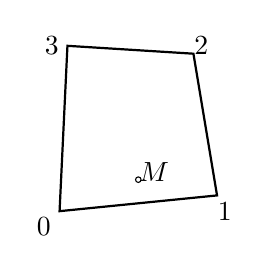
\begin{tikzpicture}
%\draw[step=0.5cm,gray,very thin] (0,0) grid (4,4); %background grid
\draw[thick] (1,1) -- (3,1.2) -- (2.7,3) -- (1.1,3.1) -- cycle;  
\node[] at (0.8,0.8) {0};
\node[] at (3.1,1) {1};
\node[] at (2.8,3.1) {2};
\node[] at (0.9,3.1) {3};
\node[] at (2.2,1.5) {$M$};
\draw (2.,1.4) circle (1pt);
\end{tikzpicture}\\
\end{center}

Several rather simple options exist:
\begin{itemize}
\item we could subdivide the quadrilateral into two triangles and check whether point $M$ is inside any of them (as it turns out, 
this problem is rather straightforward for triangles. Simply google it.)
\item We could check that point $M$ is always on the left side of segments $0\rightarrow 1$, $1\rightarrow 2$, $2\rightarrow 3$, $3\rightarrow 0$.
\item ...  
\end{itemize}

Any of these approaches will work although some might be faster than others. In three-dimensions all will however become 
cumbersome to implement and might not even work at all. Fortunately, there is an elegant way to answer the question, as 
detailed in the following subsection.

%-------------------------------------------
\subsubsection{Three-dimensional space}

If point $M$ is inside the quadrilateral, there exist a set of reduced coordinates $r,s,t\in[-1:1]^3$ such that 

\[
\sum_{i=1}^4 N_i(r_M,s,t) x_i = x_M
\quad\quad\quad
\sum_{i=1}^4 N_i(r_M,s,t) y_i = y_M
\quad\quad\quad
\sum_{i=1}^4 N_i(r_M,s,t) z_i = z_M
\]
This can be cast as a system of three equations and three unknowns. Unfortunately, each shape function $N_i$ 
contains a term $rst$ (as well as $rs$, $rt$, and $st$) so that it is not a linear system and standard techniques
are not applicable. 
We must then use an iterative technique: the algorithm starts with a guess for values $r,s,t$ and 
improves on their value iteration after iteration. 

The classical way of solving nonlinear systems of equations is Newton's method. 
\index{general}{Newton's method}
We can rewrite the equations above as ${\bm F}(r,s,t)=0$:
\begin{eqnarray}
\sum_{i=1}^8 N_i(r,s,t) x_i - x_M&=&0 \nonumber\\
\sum_{i=1}^8 N_i(r,s,t) y_i - y_M&=&0 \nonumber\\
\sum_{i=1}^8 N_i(r,s,t) z_i - z_M&=&0
\end{eqnarray}
or,
\begin{eqnarray}
F_r(r,s,t)&=&0 \nonumber\\
F_s(r,s,t)&=&0 \nonumber\\
F_t(r,s,t)&=&0 \nonumber
\end{eqnarray}

so that we now have to find the zeroes of continuously differentiable functions ${\bm F}:\mathbb{R} \rightarrow \mathbb{R}$.
The recursion is simply:
\[
\left(
\begin{array}{c}
r_{k+1} \\s_{k+1} \\ t_{k+1}
\end{array}
\right)
=
\left(
\begin{array}{c}
r_{k} \\s_{k} \\ t_{k}
\end{array}
\right)
- J_F(r_k,s_k,t_k) ^{-1} 
\left(
\begin{array}{c}
F_r(r_k,s_k,t_k) \\
F_s(r_k,s_k,t_k)\\
F_t(r_k,s_k,t_k)
\end{array}
\right)
\]
where $J$ the Jacobian matrix:
\begin{eqnarray}
J_F(r_k,s_k,t_k)
&=&
\left(
\begin{array}{ccc}
\frac{\partial F_r}{\partial r}(r_k,s_k,t_k) & \frac{\partial F_r}{\partial s}(r_k,s_k,t_k) & \frac{\partial F_r}{\partial t}(r_k,s_k,t_k) \\\\
\frac{\partial F_s}{\partial r}(r_k,s_k,t_k) & \frac{\partial F_s}{\partial s}(r_k,s_k,t_k) & \frac{\partial F_s}{\partial t}(r_k,s_k,t_k) \\\\
\frac{\partial F_t}{\partial r}(r_k,s_k,t_k) & \frac{\partial F_t}{\partial s}(r_k,s_k,t_k) & \frac{\partial F_t}{\partial t}(r_k,s_k,t_k) 
\end{array}
\right) \nonumber\\
&=&
\left(
\begin{array}{ccc}
\sum\limits_{i=1}^8 \frac{\partial N_i}{\partial r}(r_k,s_k,t_k) x_i &
\sum\limits_{i=1}^8 \frac{\partial N_i}{\partial s}(r_k,s_k,t_k) x_i &
\sum\limits_{i=1}^8 \frac{\partial N_i}{\partial t}(r_k,s_k,t_k) x_i \\
\sum\limits_{i=1}^8 \frac{\partial N_i}{\partial r}(r_k,s_k,t_k) y_i &
\sum\limits_{i=1}^8 \frac{\partial N_i}{\partial s}(r_k,s_k,t_k) y_i &
\sum\limits_{i=1}^8 \frac{\partial N_i}{\partial t}(r_k,s_k,t_k) y_i \\
\sum\limits_{i=1}^8 \frac{\partial N_i}{\partial r}(r_k,s_k,t_k) z_i &
\sum\limits_{i=1}^8 \frac{\partial N_i}{\partial s}(r_k,s_k,t_k) z_i &
\sum\limits_{i=1}^8 \frac{\partial N_i}{\partial t}(r_k,s_k,t_k) z_i 
\end{array}
\right) \nonumber 
\end{eqnarray}
In practice, we solve the following system:
\[
J_F(r_k,s_k,t_k) 
\left[  
\left(
\begin{array}{c}
r_{k+1} \\s_{k+1} \\ t_{k+1}
\end{array}
\right)
-
\left(
\begin{array}{c}
r_{k} \\s_{k} \\ t_{k}
\end{array}
\right)
\right]=-
\left(
\begin{array}{c}
F_r(r_k,s_k,t_k) \\
F_s(r_k,s_k,t_k)\\
F_t(r_k,s_k,t_k)
\end{array}
\right)
\]
Finally, the algorithm goes as follows:
\begin{itemize}
\item set guess values for $r,s,t$ (typically 0)
\item loop over k=0,...
\item Compute rhs= $-{\bm F}(r_k,s_k,t_k)$ 
\item Compute matrix $J_F(r_k,s_k,t_k)$
\item solve system for $(dr_k,ds_k,dt_k)$
\item update $r_{k+1}=r_k+dr_k$, $s_{k+1}=s_k+ds_k$, $t_{k+1}=t_k+dt_k$ 
\item stop iterations when $(dr_k,ds_k,dt_k)$ is small
\item if $r_k,s_k,t_k\in[-1,1]^3$ then $M$ is inside.
\end{itemize}
This method converges quickly but involves iterations, and multiple solves of $3\times 3$ systems which, 
when carried out for each marker and at each time step can prove to be expensive. 
A simple modification can be added to the above algorithm: iterations should be carried out {\it only}
when the point $M$ is inside of a cuboid of size $[\min\limits_i{x_i}:\max\limits_i{x_i}]\times[\min\limits_i{y_i}:\max\limits_i{y_i} ]
\times[\min\limits_i{z_i}:\max\limits_i{z_i}]$ where the sums run over the vertices of the element. 
In 2D this translates as follows: only carry out Newton iterations when $M$ is inside the red rectangle!
\begin{center}
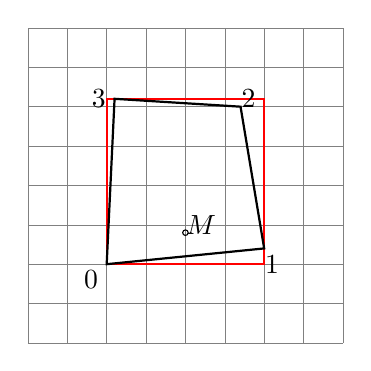
\begin{tikzpicture}
\draw[step=0.5cm,gray,very thin] (0,0) grid (4,4); %background grid
\draw[thick,red] (1,1) -- (3,1) -- (3,3.1) -- (1,3.1) -- cycle;  
\draw[thick] (1,1) -- (3,1.2) -- (2.7,3) -- (1.1,3.1) -- cycle;  
\node[] at (0.8,0.8) {0};
\node[] at (3.1,1) {1};
\node[] at (2.8,3.1) {2};
\node[] at (0.9,3.1) {3};
\node[] at (2.2,1.5) {$M$};
\draw (2.,1.4) circle (1pt);
\end{tikzpicture}\\
\end{center}

Note that the algorithm above extends to high degree elements such as $Q_2$ and higher, even with curved sides.


\todo[inline]{write about case when element is rectangle/cuboid}


 %---------
\newpage %-----------------------------------------------------------------------------------------
\subsection{Error measurements and convergence rates} \index{$L_1$ norm}
\index{$L_2$ norm}
\index{$H^1$ norm}

What follows is written in the case of a two-dimensional model. Generalisation to
3D is trivial. What follows is mostly borrowed from \cite{thmk14}.

When measuring the order of accuracy of the primitive variables $\vec{v}$ and $p$,
it is standard to report errors in both the $L_1$ and the $L_2$ norm.
For a scalar quantity $\Psi$, the $L_1$ and $L_2$ norms are computed as
\[
\norm{\Psi}_1 = \int_V |\Psi| dV
\quad\quad
\quad\quad
\norm{\Psi}_2 = \sqrt{ \int_V \Psi^2 dV }
\]
For a vector quantity $\vec{k}=(k_x,k_y)$ in a two-dimensional space,
the $L_1$ and $L_2$ norms are defined as:
\[
\norm{\vec{k}}_1 = \int_V (|k_x|+|k_y|) dV
\quad\quad
\quad\quad
\norm{\vec{k}}_2 = \sqrt{ \int_V (k_x^2+k_y^2) dV }
\]
To compute the respective norms
the integrals in the above norms can be approximated by splitting them
into their element-wise contributions. The element volume integral can then
be easily computed by numerical integration using Gauss-Legendre quadrature.

The respective $L_1$ and $L_2$ norms for the pressure error can be evaluated via
\[
e_p^h|_1 = \sum_{i=1}^{n_e} \sum_{q=1}^{n_q} |e_p^h(\vec{r}_q)| w_q |J_q|
\quad\quad
\quad\quad
e_p^h|_2=\sqrt{ \sum_{i=1}^{n_e} \sum_{q=1}^{n_q} |e_p^h(\vec{r}_q)|^2 w_q |J_q| }
\]
where $e_p^h(\vec{r}_q)=p^h(\vec{r}_q) - p(\vec{r}_q)$ 
is the pressure error evaluated at the $q$-th quadrature associated with
the $i$th element. $n_e$ and $n_q$ refer to the number of elements and
the number of quadrature points per element.
$w_q$ and $J_q$ are the quadrature weight of the Jacobian associated with
point $q$.

The velocity error $e_{\vec v}^h$ is evaluated using the following two norms
\[
e_{\vec{v}}^h|_1 = \sum_{i=1}^{n_e} \sum_{q=1}^{n_q} [ |e_u^h(\vec{r}_q)| + |e_v^h(\vec{r}_q)| ]    w_q |J_q|
\quad\quad
\quad\quad
e_{\vec v}^h|_2=\sqrt{ \sum_{i=1}^{n_e} \sum_{q=1}^{n_q} \left[ |e_u^h({\bm r}_q)|^2 +  e_v^h({\bm r}_q)|^2 \right] w_q |J_q| }
\]
where $e_u^h(\vec{r}_q)=u^h(\vec{r}_q) - u(\vec{r}_q)$ and $e_v^h(\vec{r}_q)=v^h(\vec{r}_q)-v(\vec{r}_q)$.




\index{$H^1(\Omega)$ space} \index{$H^1$ norm} \index{$H^1$ semi-norm}
Another norm is very varely used in the geodynamics literature but is preferred in the 
Finite Element literature: the so-called $H^1$ norm. The mathematical basis for this
norm and the nature of the $H^1(\Omega)$ Hilbert space is to be found in many FE books \cite{dohu03,john16,hugh}.
This norm is expression is expressed as follows for a function $f$ such that $f,|\nabla f|\in L^2(\Omega)$
\footnote{\url{https://en.wikipedia.org/wiki/Sobolev_space}}
\[
\norm{f}_{H^1} = \left( \int_\Omega ( |f|^2 + |\nabla f|^2  ) d\Omega   \right)^{1/2}
\]
We then have 
\[
e_{\vec v}^h|_{H^1} = \norm{\vec{v}^h-\vec{v}}_{H^1} = \sqrt{
\sum\limits_{i=1}^d 
\int_\Omega  
\left[
({v}_i^h-{v}_i)^2
+
\vec\nabla(v_i^h-v_i)\cdot\vec\nabla(v_i^h-v_i) 
\right] d\Omega   
}
\]
where $d$ is the number of dimensions.
Note that sometimes the following semi-norm is used \cite{dobo04,bodg06}:
\[
e_{\vec v}^h|_{H^1} = \norm{\vec{v}^h-\vec{v}}_{H^1} = \sqrt{
\sum\limits_{i=1}^d 
\int_\Omega  
\left[
\vec\nabla(v_i^h-v_i)\cdot\vec\nabla(v_i^h-v_i) 
\right] d\Omega   
}
\]
 

When computing the different error norms for $e_p$ and $e_{\vec v}$ for a set of numerical experiments with
varying resolution $h$ we expect the error norms to follow the following relationships:
\[
e_{\vec v}^h|_1 = C h^{rvL_1} 
\quad\quad\quad\quad
e_{\vec v}^h|_2 = C h^{rvL_2} 
\quad\quad\quad\quad 
e_{\vec v}^h|_{H^1} = C h^{rvH^1}
\]
\[
e_p^h|_1 = C h^{rpL_1} 
\quad\quad\quad 
e_p^h|_2 = C h^{rpL_2}
\]
where $C$ is a resolution-independent constant
and $rpXX$ and $rvXX$ are the convergence rates for
pressure and velocity in various norms, respectively. 
Using linear regression on the logarithm of the respective error norm and the resolution $h$,
one can compute the convergence rates of the numerical solutions.

As mentioned in \cite{dobo04}, when finite element solutions converge at
the same rates as the interpolants we say that the method is optimal, i.e.:
\index{optimal rate}

\[
e_{\vec v}^h|_{L_2} = {\cal O}(h^3)
\quad\quad\quad\quad
e_{\vec v}^h|_{H^1} = {\cal O}(h^2)
\quad\quad\quad\quad
e_{p}^h|_{L_2} = {\cal O}(h^2)
\]

%\begin{itemize}
%\item For $Q_1P_0$, the theoretical lower bound for $r_v'$ is 2 and for $r_p'$ it is 1
%\item For $Q_2P_{-1}$, the theoretical lower bound for $r_v'$ is 3 and for $r_p'$ it is 2
%\end{itemize}
We note that when using discontinuous pressure space
(e.g., $P_0$, $P_{-1}$), these bounds remain valid even
when the viscosity is discontinuous provided that the element boundaries conform to the discontinuity.

 
\subsubsection{About extrapolation}
\index{Extrapolation}

{\it Section contributed by W. Bangerth and part of Thieulot \& Bangerth [in prep.]}

In a number of numerical benchmarks we
want to estimate the error $X_h-X^\ast$ between a quantity $X_h$ computed
from the numerical solution $\vec{u}_h,p_h$ and the corresponding value
$X$ computed from the exact solution $\vec{u},p$. Examples of such quantities
$X$ are the root mean square velocity $v_{rms}$, but it could also be a mass flux
across a boundary, an average horizontal velocity at the top boundary, or
any other scalar quantity.

If the exact solution is known, then one can of course compute $X$ from it.
On the other hand, we would of course like to assess convergence also in
cases where the exact solution is not known. In that case, one can compute
an \textit{estimate} $X^\ast$ for $X$ by way of \textit{extrapolation}.
To this end, we make the assumption that asymptotically, $X_h$ converges to
$X$ at a fixed (but unknown) rate $r$, so that
\begin{equation}
  \label{eq:extrapolation-1}
  e_h=|X_h-X| \approx C h^r.
\end{equation}
Here, $X$, $C$ and $r$ are all unknown constants to be determined, although
we are not really interested in $C$.
We can evaluate $X_h$ from the numerical solution
on successively refined meshes with mesh sizes $h$, $h/2$, and $h/4$. Then,
in addition to \eqref{eq:extrapolation-1} we also have
\begin{eqnarray}
  \label{eq:extrapolation-2}
  e_{h/2}=|X_{h/2}-X| \approx C \left(\frac h2\right)^r,
  \\
  \label{eq:extrapolation-3}
  e_{h/4} =|X_{h/4}-X| \approx C \left(\frac h4\right)^r.
\end{eqnarray}
Taking ratios of equations \eqref{eq:extrapolation-1}--\eqref{eq:extrapolation-3},
and replacing the unknown $X$ by an \textit{estimate} $X^\ast$, we then
arrive at the following equation:
\begin{equation*}
\frac{|X_h-X^\star|}{|X_{h/2}-X^\star|}
=
\frac{|X_{h/2}-X^\star|}{|X_{h/4}-X^\star|}=2^r.
\end{equation*}
If one assumes that $X_h$ converges to $X$ uniformly either from above or
below (rather than oscillate around $X$), then this equation allows us
to solve for $X^\ast$ and $r$:
\begin{equation*}
X^\star = \frac{X_h X_{h/2}-X_{h/2}^2}{X_h - 2 X_{h/2} + X_{h/4}}, \qquad\qquad
r = \log_2 \frac{X_{h/2}-X^\star}{X_{h/4}-X^\star}.
\end{equation*}
In the determination of $r$, we could also have used $X_h$ and $X_{h/2}$,
but using $X_{h/2}$ and $X_{h/4}$ is generally more reliable because
the higher order terms we have omitted in \eqref{eq:extrapolation-1} are less
visible on finer meshes.

 %-----------------------------
\newpage %-----------------------------------------------------------------------------------------
\subsection{The initial temperature field} \subsubsection{Single layer with imposed temperature b.c.}

Let us take a single layer of material characterised by
a heat capacity $c_p$, a heat conductivity $k$
and a heat production term $H$.

\begin{center}
\includegraphics[width=5cm]{images/initial_temperature/tempcond.png}
\end{center}

The Heat transport equation writes
\[
\rho c_p ( \frac{\partial T}{\partial t} + {\vec v} \cdot {\vec \nabla} { T}) = 
{\vec \nabla} \cdot (k {\vec \nabla} T) + \rho H
\]
At steady state and in the absence of a velocity field, and assuming
that the material properties to be independent of time and space, and that
there is no heat production ($H=0$), this equation
simplifies to
\[
\Delta T =0 
\]
Assuming the layer to be parallel to the $x$-axis, this yields to write
\[
T(x,y)=T(y)=\alpha T+ \beta
\]
In order to specify the constants $\alpha$ and $\beta$, we need two constraints.

At the bottom of the layer $y=y_b$ a temperature $T_b$ is prescribed while a temperature
$T_t$ is prescribed at the top with $y=y_t$. This ultimately yields a temperature field in
the layer given by
\[
\boxed{
T(y) = \frac{T_t-T_b}{y_t-y_b}(y-y_b) + T_b
}
\]

If now the heat production coefficient is not zero, the differential equation
reads
\[
 k \Delta T + H = 0 
\]
The temperature field is then expected to be of the form
\[
T(y)= - \frac{H}{2k} y^2 + \alpha y + \beta 
\]
Supplied again with the same boundary conditions, this leads to
\[
\beta=T_b + \frac{H}{2k} y_b^2 - \alpha y_b
\]
ie,
\[
T(y) = -\frac{H}{2k} (y^2-y_b^2) + \alpha (y-y_b) + T_b
\]
and finally
\[
\alpha =  \frac{T_t-T_b}{y_t-y_b}  + \frac{H}{2k}(y_b+y_t)
\]
or,
\[
T(y) = -\frac{H}{2k} (y^2-y_b^2) + \left( \frac{T_t-T_b}{y_t-y_b}  + \frac{H}{2k}(y_b+y_t)   \right) (y-y_b) + T_b
\]

Taking $H=0$ in this equation obviously yields the temperature field obtained previously.
Taking $k=2.25$, $T_t=0C$, $T_b=550C$, $y_t=660km$, $y_b=630km$ yields the following
temperature profiles and heat fluxes when the heat production $H$ varies:
\begin{center}
\includegraphics[width=5cm]{images/initial_temperature/temperature1.pdf}
\includegraphics[width=5cm]{images/initial_temperature/heatflux1.pdf}
\end{center}
Looking at the values at the top, which are somewhat estimated to be
about $55-65mW/m^2$ \cite[table 8.6]{jama}, one sees that value $H=0.8e-6$ yields a very acceptable
heat flux.
Looking at the bottom, the heat flux is then about $0.03W/m^2$
which is somewhat problematic since the heat flux at the Moho
is reported to be somewhere between 10 and 20 $mW/m^2$ in \cite[table 7.1]{jama}.


%-----------------------------------------------------
\subsection{Single layer with imposed heat flux b.c.}

Let us now assume that heat fluxes are imposed at the top and bottom of the layer:
\begin{center} 
\includegraphics[width=5cm]{images/initial_temperature/tempcond2.png}
\end{center}

We start again from the ODE
\[
k \Delta T + H = 0 
\]
but only integrate it once:
\[
k \frac{dT}{dy}  + H y + \alpha  = 0 
\]
At the bottom $q=k(dT/dy)|_{y=y_b} = q_b$ and at the top
$q=k(dT/dy)|_{y=y_t} = q_t$ so that 

\todo[inline]{to finish}


 
%-----------------------------------------------------
\subsection{Single layer with imposed heat flux and temperature b.c. }

\begin{center}
\includegraphics[width=5cm]{images/initial_temperature/tempcond3.png}
\end{center}

\todo[inline]{to finish}


%---------------------------------------------------------------
\subsubsection{Half cooling space}

%---------------------------------------------------------------
\subsubsection{Plate model}

%---------------------------------------------------------------
\subsubsection{McKenzie slab}










 %---------------------------
\newpage %-----------------------------------------------------------------------------------------
\subsection{Kinematic boundary conditions}\label{kin_bc} \index{general}{Essential Boundary Conditions}
\index{general}{Natural Boundary Conditions}

Boundary conditions come in two basic flavors: essential and natural.
\begin{itemize}
\item Essential bcs directly affect DOFs, and are imposed on the FEM matrix. 
\item Natural bcs do not directly affect DOFs and are imposed on the right-hand side vector.
\end{itemize}

\subsubsection{In-out flux boundary conditions for lithospheric models}

\begin{center}
\includegraphics[width=8cm]{images/boundary_conditions/bc1}\\
\includegraphics[width=8cm]{images/boundary_conditions/drawing.png}
\end{center}

The velocity on the side is given by
\begin{eqnarray}
u(y) &=& v_{ext} \quad\quad y<L_1 \nn\\
u(y) &=& \frac{v_{in}-v_{ext}}{y_2-y_1}(y-y_1) + v_{ext} \quad\quad y_1<y<y_2 \nn\\
u(y) &=& v_{in} \quad\quad y>y_2 \nn
\end{eqnarray}
The requirement for volume conservation is:
\[
\Phi=\int_{0}^{L_y} u(y) dy = 0
\]
Having chosen $v_{in}$ (the velocity of the plate), one can then compute $v_{ext}$
as a function of $y_1$ and $y_2$.

\begin{eqnarray}
\Phi
&=&\int_{0}^{y_1} u(y) dy  +\int_{y_1}^{y_2} u(y) dy +\int_{y_2}^{L_y} u(y) dy \nn\\
&=& v_{ext} y_1  + \frac{1}{2}(v_{in}+v_{ext})(y_2-y_1) + (L_y-y_2) v_{in} \nn\\
&=& v_{ext} [y_1 + \frac{1}{2}(y_2-y_1) ] + v_{in} [ \frac{1}{2}(y_2-y_1)  + (L_y-y_2) ] \nn\\
&=& v_{ext}\frac{1}{2} (y_1 + y_2 ) + v_{in} [ L_y - \frac{1}{2}(y_1+y_1) ] \nn
\end{eqnarray}
and finally
\begin{mdframed}[backgroundcolor=blue!5]
\[
v_{ext} = -v_{in} \frac{ L_y - \frac{1}{2}(y_1+y_1)}{ \frac{1}{2} (y_1 + y_2 ) }
\]
\end{mdframed}

Note that in some cases applying free slip boundary conditions on a curved boundary with a triangular mesh 
can be problematic as explained in Dione \etal (2013) \cite{ditu13}.

\Literature \cite{ensg82}
 %--------------------
\newpage %-----------------------------------------------------------------------------------------
\subsection{Computing gradients - the recovery process} 
write about recovering accurate strain rate components and heat flux components on the nodes.

Let $\vec g(\vec r)$  be the desired nodal 
field which we want to be the continuous $Q_1$ representation of the field $\vec \nabla f^h$.
Since the derivative of the shape function does not exist on the nodes we need to design
an algorithm do do so. This problem is well known and has been 
investigated %\cite{XX.XXX}
\improvement{refs!}.
The main standard techniques are listed hereafter.


%..............................
\subsubsection{Global recovery}

The global recovery approach is rather simple: we wish to find $\vec g^h$
such that it satisfies
\[
\int_\Omega \phi \vec g^h \; d\Omega  = \int_\Omega \phi \vec\nabla f^h \; d\Omega 
\quad\quad \forall \phi
\] 
We will then successively replace $\phi$ by all the shape functions $N_i$ 
and since we have $g^h=\sum_j N_i g_i$ we then obtain
\[
\sum_j \int N_i N_j d\Omega g_i = \int N_i  \vec\nabla f^h \; d\Omega 
\]
or, 
\[
\mathbb{M} \cdot \vec{\cal G} = \vec f
\]



%..................................................
\subsubsection{Local recovery - centroid average over patch}





%..................................................
\subsubsection{Local recovery - nodal average over patch}

Let $j$ be the node at which we want to compute $\vec g$.
Then 
\[
\vec g_j = \vec g(\vec r_j) = 
\frac{\sum\limits_{ e \text{ adj. to }j} |\Omega_e| (\vec\nabla f)_e(\vec r_j) }{\sum |\Omega_e|}
\]
where $|\Omega_e|$ is the volume of the element and $(\vec\nabla f^h)_e(\vec r_j)$
is the gradient of $f$ as obtained with the shape functions inside element $e$ and 
computed at location $\vec r_j$.

%........................................................
\subsubsection{Local recovery - least squares over patch}



%........................................................
\subsubsection{Link to pressure smoothing}

When the penalty method is used to solve the Stokes equation, the pressure
is then given by $p=-\lambda \vec\nabla \cdot \vec v$. As explained in 
section \ref{sec_penalty}, the velocity is first obtained and the pressure 
is recovered by using this equation as a postprocessing step. Since the divergence 
cannot be computed easily at the nodes, the pressure is traditionally computed 
in the middle of the elements, yielding an elemental pressure field (remember, 
we are talking about $Q_1P_0$ elements here -- bi/tri-linear velocity, discontinuous
constant pressure)



\improvement{tie to fieldstone 12}

 %-------------------------
\newpage %-----------------------------------------------------------------------------------------
\subsection{Tracking materials and/or interfaces} \begin{flushright} {\tiny {\color{gray} tracking.tex}} \end{flushright}

Unless using a fully Lagrangian formulation, one needs an additional numerical method to represent/track
the various materials present in an undeformable (Eulerian) mesh.
The figure below (by B. Hillebrand) illustrates the three main methods used in geodynamics.

\begin{center}
\includegraphics[width=15cm]{images/tracking/tracking}
\end{center}

Note that what follows is applicable to FEM, FDM, etc ...


A typical test for advection algorithm is the Zalesak disk \cite{zale79}. It is a two dimensional test 
problem of solid body rotation with a constant angular velocity $\omega$ (in rad/sec):

\begin{center}
\includegraphics[width=6cm]{images/tracking/zale79a}
\includegraphics[width=6cm]{images/tracking/zale79b}\\
{\tiny Taken from \cite{zale79}. Left: Schematic representation of two dimensional 
solid body rotation problem. The field inside the cut out has value 3 and it is 1
outside. The rotational speed is such that one full revolution is effected in 
628 cycles. The width of the gap separating the two halves of the cylinder,
as well as the maximum extent of the "bridge" connecting the two halves, is 5 cells.
Right: Perspective view of initial conditions for the two dimensional! solid body rotation
problem. Note that only a $50\times50$ portion of the mesh centered on the cylinder is displayed.}
\end{center}

This benchmark is widely used in the literature \cite{stco91,supu00,vasv05,dilp06,basd08,zhbl14}.
Note that the Zalesak disc is often supplemented with a cone and a Gaussian features:

\begin{center}
\includegraphics[width=6cm]{images/tracking/leve96}\\
{\tiny Taken from \cite{leve96}. Initial data for solid rotation tests}
\end{center}

%..............................................
\subsubsection{The Particle-in-cell technique}\label{ss:pic}
\index{general}{Particle-in-Cell}  
\index{general}{Marker-and-Cell} 
\index{general}{PIC} 
\index{general}{MAC}

\begin{remark}
The terms 'particle' and 'marker' are commonly (and unfortunately) interchangeably used in the literature 
in the context of the particle-in-cell technique. However, one should be aware that the marker-and-cell (MAC) 
technique is something different: it was invented in the early 60's at the Los Alamos Laboratories by 
Harlow and Welch (1965) \cite{hawe65}. For more information on MAC see the review paper 
by McKee \etal (2008) \cite{mctf08}. 
Also, Tackley and King (2003) \cite{taki03} talk about the tracer-ratio method in the context of PIC... 
\end{remark}

The Particle-in-cell method is by far the most widely used in computational geodynamics. 
In its most basic form it is a rather simple method to implement and this probably owes to its success
and early adoption \cite{popo92}  in non-parallel codes such as \sopale \cite{full95}, 
I2VIS \cite{geyu03} or \citcoms \cite{mczh04} (Appendix~\ref{app:codes}).
It has been implemented in \aspect{} \cite{galh18} and the inherent load balancing issues arising from the 
parallel implementation as well as from the use of Adaptive Mesh Refinement are discussed. 
It has also been implemented in the MILAMIN code \cite{daks08} to study LLSVPs \cite{musd15}.

\begin{center}
\includegraphics[width=8cm]{images/tracking/crsg12}\\
{\captionfont One of the main problems of the PIC method is the fact that the interface 
between the fluid is not tracked explicitely, and if one uses a random distribution of 
particles the black dotted line reprensents the 'real' interface between the fluids 
while the red line is liekly to be the interface one would obtain based on the 
distribution of particles. Taken from Crameri \etal (2012) \cite{crsg12}.}
\end{center}

Samuel (2018) \cite{samu18} does a great job at explaining 
the core problem with PIC: {\it the method requires the method requires particle-mesh 
and mesh-particle mappings to be specified. These critical operations constitute a
major source of inaccuracy in the PIC solution \cite{mona85,dumg11,thmk14}. 
Indeed, while the Lagrangian advection alone is not prone
to significant numerical diffusion, particle–mesh mappings can introduce 
important amounts of dissipation. This is particularly true
when the spatial distribution of particles is not homogeneous, leading 
to areas in the vicinity of gridpoints that are not sufficiently
well sampled by particles, and other regions where the domain is
oversampled by particles. This recurrent sampling problem develops 
in regions characterized by strong deformation, and concerns
both compressible and incompressible flow \cite{waav15,pukp16}. 
The non-homogeneous sampling has two main
origins. \\
- The first one corresponds to inaccuracies in advecting the
Lagrangian particles \cite{meje04}. This aspect has drawn
the attention of a few recent studies \cite{waav15,pukp16}, 
which have proposed the use of conservative schemes to
map velocity components from the Eulerian grid to the Lagrangian
particles during their advection. Such schemes have shown to significantly 
improve the accuracy of the interpolation, and result in
a considerably more homogeneous spatial sampling. \\
- The second origin, which has received less attention, is related to the deforming
nature of the flow \cite{modm03}, and is completely independent 
of the accuracy of the numerical methods for interpolating
the velocities at particles’ locations. In fact, for a given velocity
field, particles should travel along their characteristics, and even in
the case of incompressible flows, the distance between characteristics 
can vary in general, and can strongly diverge or converge in
regions characterized by strong deformation. This naturally leads to
the development of a non-homogeneous spatial distribution of the
Lagrangian particles, even if the particles locations are perfectly
known.}



The basic methodology goes as follows:
\begin{enumerate}
\item distribute particles in the domain
\item assign a material identity (and/or any other quantity) to each of them
\item project particle quantities of the Eulerian nodes of the mesh
\item solve the Stokes equations for a new velocity field
\item interpolate the velocity onto the particles
\item move the particles with their respective velocities 
\item go back to step 3
\end{enumerate}  

As it turns out each step above needs to be carefully executed and is more difficult than it 
first looks. 

\paragraph{Distributing particles in the domain}. Let us assume we wish to distribute $N_p$ particles
in the domain. How large must $N_p$ be? To simplify, one end member could be 'as many particles as possible that fit in memory' 
while the other end member could be 'one per element/cell on average'. While the former does not necessarily guarantee a 
desired accuracy while being CPU and memory intensive, the latter will certainly lead to zones in the domain void 
of particles which will be problematic since the projection onto the mesh might yield zero values or very inaccurate values.
How many particles (per element/cell) will be enough?
Also, should the particles be randomly distributed in the domain or on some kind of regular grid? 
See \stone 13.

Taken from Tackley and King (2003) \cite{taki03}: "Tracers are initialized on a regular grid 
with each tracer perturbed from its grid position by a random amount of up to
$\pm$ half a grid spacing, in order to eliminate artifacts due to tracer alignment."


\paragraph{Averaging and projection}. This is a very critical step. Unfortunately, there is no community-wide
agreed-upon method. The problem at hand boils down to: at a given location $(\vec r)$ in space I need a
the value of a field which is carried by the particles. 
The first step is to find the particle(s) close to this point. If done naively, this is a very costly affair, 
and begs the question what 'close' means. Finding all particles within a radius $R$ of point $\vec r$ can 
be done very efficiently (e.g. with linked lists, Verlet lists, ...) but the choice 
of $R$ proves to be critical:
if too small, there may not be any particle inside the circle, and if too large there may be many particles 
inside the circle and the averaging over so many particles in space will prove to be over diffusive. 
In practice, the FD or FE mesh is used to provide an indication of $R$. 
In FDM, the four cells (or quarter cells) around
a node represent the volume of space containing the particles whose properties are to be averaged \cite{dumg11} 
as illustrated in the following figure:

\begin{center}
\includegraphics[width=12cm]{images/dumg11}\\
{\captionfont Taken from \cite{dumg11}. The "4-cell" and "1-cell" schemes for projecting 
properties defined on the markers (denoted by stars) onto a node (denoted by the solid circle). 
(A) The 4-cell scheme. The support of the interpolating function $N_i$ associated
with node $i$ is indicated by the shaded region. Only markers within the support of node $i$ 
contribute to the projection operation used to define the nodal value at $i$. The shape of 
the bilinear interpolation function for node $i$ is indicated in the lower frame. 
(B) The 1-cell scheme. The thick lines in the lower frame indicate the grid used to discretize the
Stokes equations, while the thin lines indicate the grid onto which marker properties are projected. 
The 1-cell scheme utilizes a compact support of size $\Delta x \times  \Delta y$. The support 
for nodes $r$, $s$, $t$ are indicated by the shaded regions. Only markers within the nodal 
support contribute to the projection operation for that node.}
\end{center}

Given that the FEM requires to compute integrals over each element, one could assume that 
only the particles inside the element will contribute 
to the average values assigned to the quadrature points (which I coin 'elemental approach'). 

However, one could also decide to first average the properties onto the nodes
before using these nodal values to assign values to the quadrature points (which I coin 'nodal approach'). 
In this case the FDM approach seen above could apply. 

Finally, in both FDM and FEM bi/trilinear basis functions are used for the interpolation as 
they can be interpreted as weighing functions. Higher order basis functions could also be used 
but the standard $Q_2$ basis functions (Section~\ref{sec:shpfct2d})
are 2-nd order polynomials which can take negative values (as opposed to the $Q_1$ 
basis functions which are strictly positive)
and this can pose problems: in some cases, although all values to be averaged are positive, 
their weighed average can be negative.
See Section~\ref{ss:bern} for concrete examples.

\underline{nodal approach}

\underline{elemental approach (1) - piece-wise constant interpolation} 

What follows is written with simplicity in mind, although more mathematical formulations 
can be found in the literature \cite{galh18}.

Assuming that we have established a list of particles tracking a field $f(\vec r)$ inside the 
element 
%and that each particle has an 
%associated weight $w_i$ (function of the location where the average is to be computed or not), 
we must now compute their average value $<f>$. 
The simplest approach which comes to mind is the arithmetic mean ($am$):
\[
\langle f\rangle_{am} = \frac{\sum\limits_{i=1}^n f_i}{n}
\]  
where $n$ is the number of particles inside the element.
In the case where $f$ is the (mass) density $\rho$, it is indeed what should be used. 
However, turning now to viscosity $\eta$, we know that its value can vary by many orders of magnitude 
over very short distances.
It is then likely that the average runs over values spanning values between 
$10^{18}\text{Pa s}$ and $10^{25} \text{Pa s}$.
As explained in \cite{scbe08} the arithmetic averaging tends to 'favour' large values: 
if the sum runs over 
10 particles, 9 carrying the value $10^{25}$ and 1 carrying the value $10^{19}$, 
the average value is then
\[
\langle\eta\rangle = \frac{9\cdot 10^{25}+1\cdot 10^{19}}{10} \simeq 0.9\cdot 10^{25}
\]
which is much much closer to $10^{25}$ than to $10^{19}$.
Other averagings are then commonly used, namely the geometric mean ($gm$)  and the 
harmonic mean ($hm$), defined as follows:
\[
\langle f\rangle_{gm} = \left( \prod_i f_i \right)^{1/n} 
\qquad
\text{or, }
\qquad
\log_{10} \langle f \rangle_{gm} = \frac{\sum\limits_{i=1}^{n} \log_{10} f_i }{n}  
\]
and 
\[
\langle f\rangle_{hm} = \left( \frac{\sum\limits_{i=1}^n \frac{1}{f_i} }{n}  \right)^{-1}
\qquad
\text{or, }
\qquad
\frac{1}{\langle f\rangle_{hm} } = \frac{\sum\limits_{i=1}^n  \frac{1}{f_i} }{n}  
\]
The geometric mean can be seen as a form of arithmetic mean of $\log_{10}$ values, 
while the harmonic mean can be seen as 
a form of arithmetic mean of the inverse values.

Looking back at the above example, the geometric mean of the viscosities is given by 
\[
\log \langle \eta\rangle_{gm} = \frac{9\cdot 25+1\cdot 19}{10} = 24.4 
\qquad \text{or,} \qquad 
\langle \eta\rangle_{gm} \simeq 2.5 \cdot 10^{24}
\]
and the harmonic mean:
\[
\langle\eta\rangle_{hm} \simeq \left( \frac{1}{10 \cdot  10^{19}} \right)^{-1} = 10^{20}
\]
We see that the harmonic mean tends to favour the small values. Also we recover the known property:
\begin{equation}
\langle f \rangle_{am}\quad  \geq \quad
\langle f \rangle_{gm}\quad  \geq \quad
\langle f \rangle_{hm} 
\end{equation}

%When all $f_i$ are equal to $f_0$ their computed average should also be equal to $f_0$. As a consequence the 
%weights $N_i$ should fulfil the condition $\sum\limits_{i=1}^n N_i=1$.
%If all weights are equal, then $N_i=1/n$ and the averagings become:

%\begin{equation}
%\langle f\rangle_{am} = \frac{1}{n} \sum\limits_{i=1}^n f_i
%\qquad
%\langle f\rangle_{gm} = \prod_i f_i^{1/n} 
%\qquad
%\langle f\rangle_{hm} = \left( \frac{1}{n}\sum_i^n \frac{1}{\phi_i} \right)^{-1}
%\end{equation}

Once a single average value has been computed for the whole element, then 
all quadrature points are assigned this value. 


\underline{elemental approach (2) - Least Squares Interpolation } 
One can revisit this topic on the grounds that 
with high(er) order elements optimal convergence is unlikely to be reached 
if viscosity (and density) are assumed to be constant inside each element (see  
\cite{galb19}). One could therefore use the least-square method to arrive at 
a functional representation of the field inside the element which is as 
close as possible (in the least-squares sense, then) to the particle-based field. 

Thielmann \etal (2014) \cite{thmk14} use the $Q_2P_{-1}$ element and introduce an element-wise interpolation
scheme based on a least squares fitting of the particle properties and choose the functional to 
be a linear function to match the pressure space. 
They define the error $\epsilon$ such that 
\[
\epsilon^2 = \sum_{i=1}^n ( \tilde{f}(x_i,y_i)-f_i)^2
\]
with $\tilde{f}(x,y)=a+bx+cy$. 
We then look for the minimum of $\epsilon^2$, i.e. $\vec\nabla(\epsilon^2)=0$ in the $\{a,b,c\}$ space.
So 
\begin{eqnarray}
0=\frac{\partial \epsilon^2}{\partial a} 
&=& 2\sum\limits_i ( \tilde{f}(x_i,y_i)-f_i) \nn\\
&=& 2\sum\limits_i ( a + bx_i +cy_i -f_i) \nn\\
&=& 2 \left[ a \sum\limits_i 1 + b \sum\limits_i x_i + c \sum y_i - \sum\limits_i f_i \right] \nn\\
0=\frac{\partial \epsilon^2}{\partial b} &=& 2\sum\limits_i ( \tilde{f}(x_i,y_i)-f_i) x_i \nn\\
&=& 2\sum\limits_i ( a + bx_i +cy_i -f_i) x_i \nn\\
&=& 2 \left[ a \sum\limits_i x_i  + b \sum\limits_i x_i^2 + c \sum x_i y_i - \sum\limits_i x_i f_i \right]\nn\\
0=\frac{\partial \epsilon^2}{\partial c} &=& 2\sum\limits_i ( \tilde{f}(x_i,y_i)-f_i) y_i \nn\\ 
&=& 2\sum\limits_i ( a + bx_i +cy_i -f_i) y_i \nn\\
&=& 2 \left[ a \sum\limits_i y_i + b \sum\limits_i x_i y_i + c \sum y_i^2 - \sum\limits_i y_if_i \right] \nn
\end{eqnarray}
so 
\[
\left( 
\begin{array}{ccc}
\sum\limits_i 1 & \sum\limits_i x_i & \sum\limits_i y_i \\
\sum\limits_i x_i & \sum\limits_i x_i^2 & \sum\limits_i x_iy_i \\
\sum\limits_i y_i & \sum\limits_i x_i y_i & \sum\limits_i y_i^2 
\end{array}
\right)
\cdot
\left(
\begin{array}{c}
a\\
b\\
c
\end{array}
\right)
=
\left(
\begin{array}{c}
\sum\limits_i f_i \\
\sum\limits_i x_i f_i \\
\sum\limits_i y_i f_i 
\end{array}
\right)
\]

We could also then decide to use a bi-linear function $\tilde{f}$, i.e.
\[
\tilde{f}(x,y)=a+bx+cy+dxy
\]
which lies in the $Q_1$ space of Taylor-Hood quadrilateral elements. In this case the error is 
\[
\epsilon^2 
= \sum_{i=1}^n ( \tilde{f}(x_i,y_i)-f_i)^2
= \sum_{i=1}^n (a+bx_i+cy_i + dx_iy_i -f_i)^2
\]
and one has to solve a $4\times 4$ system this time:
\[
\left( 
\begin{array}{cccc}
\sum\limits_i 1 & \sum\limits_i x_i & \sum\limits_i y_i & \sum\limits_i x_iy_i\\
\sum\limits_i x_i & \sum\limits_i x_i^2 & \sum\limits_i x_iy_i & \sum\limits_i x_i^2 y_i\\
\sum\limits_i y_i & \sum\limits_i x_i y_i & \sum\limits_i y_i^2 & \sum\limits_i x_iy_i^2\\ 
\sum\limits_i x_iy_i & \sum\limits_i x_i y_i & \sum\limits_i y_i^2 & \sum\limits_i x_i^2y_i^2  
\end{array}
\right)
\cdot
\left(
\begin{array}{c}
a\\
b\\
c\\
d
\end{array}
\right)
=
\left(
\begin{array}{c}
\sum\limits_i f_i \\
\sum\limits_i x_i f_i \\
\sum\limits_i y_i f_i \\
\sum\limits_i x_i y_i f_i 
\end{array}
\right)
\]


Once this linear system (or the previous one) has been solved we have obtained the coefficients $a,b,c(,d)$ 
which allow us to compute $\tilde{f}$ anywhere inside the element, and especially 
at the quadrature points. 

\begin{remark}
Using a different (bi)linear function $\tilde{f}$ for each element 
means that it is likely to be discontinuous 
from one element to another in regions of high gradients. 
\end{remark}

There is however one drawback with this approach (linear or bi-linear alike):
in the areas of steep gradients the computed coefficients can be such that 
the function $\tilde{f}$ evaluated on a quadrature point 
is negative  which 1) would be wrong but not numerically 
dramatic for density, 2) would be wrong and physically and numerically 
problematic for viscosity (a viscosity cannot be negative, and this would 
automatically destroy the SPD nature of the viscous block of the Stokes matrix).

This problem is discussed in Thielmann \etal (2014) in Section 3.2.1 and they 
call this "Over- and Under-shooting". A simple (iteratuve) 
fix is then designed which insures that the computed value is within user-defined 
acceptable bounds. This is also mentioned in \cite{galb19} but the authors 
explain that this problem was not encountered in the context of the publication.





\begin{remark}
Two variants of the PIC methods have been proposed: the Deformable PIC (DPIC) 
by Samuel (2018) \cite{samu18}, and the multiscale PIC in \cite{asmo12}.
\end{remark}

\begin{remark}
TO BE WRITTEN.
A word about the tracer ratio method. \cite{taki03}. 
Trim \etal (2020) show a modified method 
with a tracer repositioning algorithm designed to promote even tracer
coverage \cite{trlb20}. 
\end{remark}



See Stone~67 for a concrete example of Particle-In-Cell use and a detailed 
explanation of its implementation.



%.....................................................................
\paragraph{Interpolation of the velocity onto particles}.

Once the particle $i$ has been localised inside a given element (Section~\ref{sec:amiin}) 
and its reduced coordinates $(r,s,t)$ determined, the velocity at this location can 
be computed through the basis functions:
\[
\vec\upnu_i=\sum_{k=1}^m N_i(r,s,t) \vec\upnu_k
\]
This approach is not without problem: while the nodal velocities $\vec\upnu_k$ are such 
that\footnote{for incompressible flows, of course} 
$\vec\nabla\cdot\vec\upnu=0$ (in the weak sense), the computed velocity $\vec\upnu_i$ 
is not necessarily divergence-free! In order to remedy this, a 
Conservative Velocity Interpolation (CVI) has been proposed in \cite{waav15}.
Because the complete derivations for the CVI algorithm is quite large I 
have decided to make a new section about it (Section~\ref{sec:cvi}) rather than include it 
here.

%.....................................................................
\paragraph{Moving the particles}

This is discussed in the context of the Runge-Kutta Methods, see Section~\ref{sec:rkparticles}.



%..............................................
\subsubsection{The level set function technique}
\index{general}{Level-set Method} 
\index{general}{Level-set Function} 
\index{general}{LSM} 
\index{general}{LSF} 
\index{general}{ENO}

This method was developed in the 80's by Stanley Osher and James Sethian \cite{lofo06}

The Level-set Method (LSM), as it is commonly used in Computational Fluid Dynamics -- and especially 
in Computational Geodynamics -- represents a close curve $\Gamma$ (say, in our case, the 
interface between two fluids or layers) by means of a function $\phi$ (called the level-set function, or LSF).
$\Gamma$ is then the zero level-set of $\phi$:
\begin{equation}
\Gamma = \left\{ (x,y) \; |\; \phi(x,y)=0 \right\}
\end{equation}
The convention is that $\phi>0$ inside the region delimited by $\Gamma$ and $\phi<0$ outside.
The function value indicates on which side of the
interface a point is located (negative or positive) and this is
used to identify materials. 

Furthermore, if the curve $\Gamma$ moves with a velocity $\vec \upnu$, 
then it satisfies the following equation:
\begin{equation}
\frac{\partial \phi}{\partial t} + \vec\upnu \cdot \vec\nabla \phi = 0 
\end{equation}

The level set function is generally chosen to
be a signed distance function, i.e. $|\vec\nabla \phi| = 1$ everywhere 
and its value is also the distance to the interface.

As explained in \cite{hitg14}, the level-set function $\phi$ is advected 
with the velocity $\vec\upnu$ which is obtained by solving the Stokes equations.
This velocity does not guarantee that after an advection step the signed 
distance quality of the LSF is preserved. 
The LSF then needs to be corrected, which is also called reinitialisation. 
Finally, solving the advection equation must be done in an accurate manner both in time and space,
so that so-called ENO (essentially non-oscillatory) schemes are often employed for the 
space derivative \cite{ossh91,saev10}.


The level set method has not often been used in the geodynamics 
community with some notable exceptions 
\cite{bomh06,bomh07,habm07,grbh07,zlfd08,hagr10,sunh10,suhe10,hitg14}
An overview of the method and applications can
be found in \cite{osfe01}.

Several improvements upon the original LSM have been proposed, 
such as for instance the conservative level set of \cite{zhbl14}.
The most notable difference between CLS method originally proposed by Olsson \etal \cite{olkr05,olkz07}
and standard LS method lies in the choice of LS function. Instead of the signed distance function, the
CLS methods employ the Heaviside function $H(\phi)$ 
\[
H(\phi)=
\left\{
\begin{array}{ll}
1 & \phi>0 \\
1/2 & \phi=0 \\
0 & \phi<0
\end{array}
\right.
\]
where $\phi$ is the signed distance function as in the LSM. 
In practice, a hyperbolic tangent function is used:
\[
H(\phi) = \frac{1}{2} (1+\tan (\phi/2\epsilon))
\]
where $\epsilon$ defines the spreading width of $H$. In the case where there are only 
two fluids (i.e. a single level set is sufficient), the material properties such as density and viscosity
are computed as follows:
\[
\rho=\rho_1+(\rho_2-\rho_1)H(\phi)
\]
\[
\eta=\eta_1+(\eta_2-\eta_1)H(\phi)
\]

\Literature: \cite{vasv05,vasv08,migi07,vasv05b}. 
\begin{itemize}
\item Review of level-set methods \cite{gifo18}
\item Interactive 3-D computation of fault surfaces using level sets \cite{kadt08}
\end{itemize}

%..............................................
\subsubsection{The field/composition technique \label{sec:compfield}}
\index{general}{Compositional Field}

This is the approach taken by the \aspect{} developers \cite{krhb12,hedg17}. 
Each material $i$ is represented by a compositional field $c_i$, 
which takes values between 0 and 1.
Each compositional field is then advected with the (prescribed or computed) Stokes velocity \cite{chri92}:
\begin{equation}
\frac{\partial c_i}{\partial t} + {\bm v}\cdot {\bm \nabla }c_i = 0
\end{equation}
The value at a point (Finite element node or quadrature point) is 1 if it is in the 
domain covered by the material $i$, and 0 otherwise.
In one dimension, each compositional field is a Heavyside function. 
This approach is somewhat similar to the LSM but the field is essentially 
discontinuous across the interface, which makes it very difficult to advect.  
On the plus side, compositional fields need not be reinitialised, as opposed to LSF's.

Accurate numerical advection is a notoriously difficult problem. Unless very specialised 
techniques are used it often yields undershoot ($c_i<0$) and overshoot ($c_i>0$), which 
ultimately yields mass conservation issues. Also, unless special care is taken, 
compositional fields tend to become more and more diffuse over time: the SUPG method (Section~\ref{sec:supg})
and the entropy viscosity method \cite{krhb12,ropu19} add small amounts of diffusion to dampen the under- and 
overshoots. This means that at a given point two or more compositions may have values, 
which require some form of averaging. If under- and overshoots are present, these averagings
can become very problematic and even yield meaningless quantities (e.g. negative viscosities).

One rather old and popular filtering approach is the so-called Lenardic and Kaula (1993) \cite{leka93}
filter:

\begin{center}
\includegraphics[width=6cm]{images/compositions/leka93_filter1}\\
\includegraphics[width=6cm]{images/compositions/leka93_filter2}\\
{\captionfont Taken from Lenardic and Kaula \cite{leka93}}
\end{center}

\begin{center}
\includegraphics[width=16cm]{images/compositions/leka93_filter3}\\
{\captionfont From FENICS book}
\end{center}


\begin{center}
\includegraphics[width=8cm]{images/compositions/plth13}\\
{\captionfont 
Filtering approach proposed by Lenardic and Kaula (1993). 
The composition field $C$ is assumed to vary between 0 and 1. Grid points with $C$-values 
lower than 0 and greater than 1 are set to 0 and 1, respectively (red). 
$C_{min}$ and $C_{max}$ are the minimum and maximum spurious values observed. 
Grid points whose $C$-value is lower than $|C_{min}|$ or greater than ($2-C_{max}$) 
are also set to 0 and 1, respectively (blue). 
The $C$-value of all grid points that do not exhibit spurious oscillations (green) is then corrected
according to the difference between the original average composition and that computed after the reset-
ting of the spurious values.
Taken from Plesa \etal (2013) \cite{plth13}.}
\end{center}











\Literature: \cite{vyrc13}

Entropy viscosity method \cite{gupa11}

\improvement[inline]{write about DG approach}






%..............................................
\subsubsection{The Volume-of-Fluid method} 
\index{general}{Volume-of-Fluid Method}
\index{general}{VOF}

%from Napoleon \etal
The Volume-Of-Fluid (VOF) method is a fixed-grid approach based on the one-fluid model and considers that the various immiscible fluids (or `phases') can be described as a single fluid whose local physical properties, namely density and viscosity, vary in space and time depending on the volume fraction $C_i$ of each phase $i$ 
\cite{hini81,youn82}. 

The volume fraction of each fluid intrinsically obeys $\sum \limits_{{i=1}}^n C_i = 1$ where $n$ is the number of phases. 
Typically, $C_i=1$ in grid cells filled only with fluid $i$, and $0<C_i<1$ in grid cells cross--cut by an interface. 
There are two main classes of VOF methods: methods that try to reconstruct exactly the interface between fluids (e.g. \cite{puth18}), which requires significant computational time, and methods that do not, such as in JADIM and OpenFOAM. 
With no interface reconstruction, the thickness of the interfacial region is defined by $0<C_i<1$, and typically occupies two to three grid cells. 

\cite{hini81}\cite{ropu19}

See review of the method in Robey's phd thesis \cite{robe19}.


%..............................................
\subsubsection{The method of characteristics}

\todo[inline]{ask Arie to write something}

\cite{devv00a}

%.............................................
\subsubsection{The Marker Chain method}
\index{general}{Marker Chain method} 

In two dimensions, the idea is quite simple: each interface is discretised by means of a number
of Lagrangian points (which may or may not vary in time). The points are numbered and 
connected (think of the connectivity array of a 1D FEM code). In the case of small deformations, 
and in the absence of in/out-flow boundaries, the method is reasonably trivial to implement, and 
each couple of point defines a segment (and therefore its normal vector too) which can then be used
to answer the question: "at this location, am I above or below this interface" or "am I this domain our
outside this domain" (in the case that the interface does not reach any of the boundaries).

This method becomes somewhat impractical when large deformation occurs or, for example, 
when a domain splits into two (e.g. slab break off). One interface must then become two, 
and it requires an algorithm capable of detecting the breakup of the surface and capable 
of rebuilding/patching the new ones so that they can still be used further. 
Note that in case of large deformation some markers may get further and further apart 
from each other which makes for a poor representation of the surface. New markers should then 
be added but the question of when and where must then be addressed.

Also, switching to three dimensions can prove to be very difficult or simply very 
costly: the generation of the inital marker position is trivial but their connectivity 
can be complicated to establish at startup: for instance, a Stokes sphere will require
a mesh made of triangles which maps exactly the surface of the sphere (see \cite{thie18,moma19} 
for methods on how to efficiently produce such meshes). In the case of more complex 3D geometries
this may prove nearly impossible to do. So will the problem of splitting a surface into two 
(or merging two domains). \todo{I still have pics from the old days using \douar- include} 

This method is usually coupled to Eulerian meshes (typically with FDM, but not only). 
It was used in \cite{woid78} in the context of salt domes analysis and later in \cite{chri82,chyu84}.
It is also used in \cite{vaks97} but little details are given about the algorithms used
to track and update the chain in the presence of such large deformation.
It is also used (athough coupled to level set functions) in the \douar code\cite{brtf08} 
(see Section~\ref{app:codes}). Having worked myself on this code and having had to produce 
complex initial triangulated surfaces for simulations (see for example \cite{lobh10}) it is 
easy to understand why later users of this code did implement the marker-in-cell technique.
More recently, it is used to track the free surface position in a FDM code \cite{dumy16,chmd19}.

Finally, Christensen \cite{chri92} makes the following interesting comment:  
"One might assume that different methods 
of representing the discontinuity, for example, by a tracer chain \cite{chyu84} or a cloud of 
tracers, would solve these problems. However, the difficulties 
arise not only from the way in which material boundaries are 
represented. Physically, the rate of shear strain parallel to a 
rheological boundary is discontinuous. Within the finite ele-
ment scheme such jump can only be realized at an element 
boundary. In an Eulerian scheme, where the discontinuity will 
crosscut the elements, the jump in strain rate must be approx- 
imated by a continuous variation, and effectively, the rheolog-
ical properties on both sides of the discontinuity will be 
averaged in some way within the element."

Literature: Lin \& van Keken (2006) \cite{liva05,liva06a,liva06b,kaus05,mulyukova}

%..............................................
\subsubsection{Hybrid methods}

In Braun \etal \cite{brtf08} a level set method is presented which is based on a 3-D set
of triangulated points, which makes it a hybrid between tracers and level set functions:
in the \douar code (Appendix~\ref{app:codes}) the interface is then explicitely tracked by means of the tracers while the LSF is computed 
on the FE nodes. Although very promising in theory, this method proved to be difficult to use in practice
since it requires a) a triangulation of the interfaces at $t=0$ which is not trivial if the geometries
are complex (think about a slab in 3D); b) the addition or removal of tracers because of the interface deformation
and the patching of the triangulation; c) the calculation of the distance to the interfaces for each 
FE node based on the triangle normal vectors. 
This probably explains why the Particle-In-Cell method was later implemented in this code (pers. comm.).
Note that another very similar approach is used in \cite{saev10}.



%..............................................
\subsubsection{Boundary fitted mesh}

This method is rather simple to implement and works well for small deformations. It is 
for instance used by Frehner \cite{freh14} (see online supplementary material) in which it is 
stated: "The numerical grid is set up in such a way that the interface
between different material phases (two layers in this case) coincides with element boundaries. Hence, each
element belongs to a unique material phase and no interpolation is necessary."
With such a method, each element is initally attributed a material phase/number and its material
properties do not change. 


\vspace{2cm} 

\Literature: three-dimensional front tracking method using a triangular mesh \cite{sclo03}.







 %-------------------------------
\newpage %-----------------------------------------------------------------------------------------
\subsection{Static condensation} \index{general}{Static Condensation}

The idea behind static condensation is quite simple: in some cases, there are dofs 
belonging to an element which only belong to that element. For instance, the so-called MINI 
element ($P_1^+ \times P_1$) showcases a bubble function in the middle (see section \ref{ss:pair}). 
In the following, $\vec{\cal V}^\star$ corresponds to the list of such dofs inside an element.
The discretised Stokes equations on any element looks like:

\begin{equation}
\left(
\begin{array}{ccc}
\K   & L & \G \\
L^T & \K^\star  & H \\
\G^T & H^T & 0
\end{array}
\right)_e
\left(
\begin{array}{c}
\vec{\cal V} \\ \vec{\cal V}^\star \\ \vec{\cal P}
\end{array}
\right)_e
=
\left(
\begin{array}{c}
\vec{f} \\ \vec{f}^\star \\ \vec{h}
\end{array}
\right)_e
\end{equation}
This is only a re-writing of the elemental Stokes matrix where the matrix $\K$ has been 
split in four parts.
Note that the matrix $\K^\star$ is diagonal.\todo{check}

This can also be re-written in non-matrix form:
\begin{eqnarray}
\K \cdot \vec{\cal V} + L \cdot \vec{\cal V}^\star + \G \cdot \vec{\cal P} &=& \vec{f} \\
L^T V + K^\star \cdot  \vec{\cal V}^\star + H \cdot \vec{\cal P} &=& \vec{f}^\star \\
\G^T \cdot \vec{\cal V} + H^T \vec{\cal V}^\star &=& \vec{h}
\end{eqnarray}
The $\vec{\cal V}^\star$ in the second equation can be isolated:
\[
\vec{\cal V}^\star = \K^{-\star} \cdot ( \vec{f}^\star - L^T \cdot \vec{\cal V} - H \cdot \vec{\cal P})
\]
and inserted in the first and third equations:
\begin{eqnarray}
\K \cdot \vec{\cal V} + L \left[ \K^{-\star} ( \vec{f}^\star - L^T \cdot \vec{\cal V} - H \cdot \vec{\cal P} )  \right] + \G \cdot \vec{\cal P} &=& \vec{f} \\
\G^T \cdot \vec{\cal V} + H^T \left[  \K^{-\star} ( \vec{f}^\star - L^T \cdot \vec{\cal V} - H \cdot \vec{\cal P}) \right]  &=& \vec{h}
\end{eqnarray}
or,
\begin{eqnarray}
(\K-L\cdot \K^{-\star} \cdot L^T)\cdot \vec{\cal V} + (G-L\cdot \K^{-\star} \cdot H) \cdot \vec{\cal P} &=& \vec{f}-L\cdot \K^{-\star} \cdot \vec{f}^\star \\
(G^T -H^T\cdot \K^{-\star}\cdot  L^T ) \cdot \vec{\cal V}  - 
(H^T \cdot \K^{-\star} \cdot H )\cdot \vec{\cal P}   &=& \vec{h} -H^T\cdot \K^{-\star}\cdot \vec{f}^\star
\end{eqnarray}
i.e.
\begin{eqnarray}
\underline{\K} \cdot \vec{\cal V} + \underline{\G}\cdot \vec{\cal P} &=& \underline{\vec{f}} \\
\underline{\G}^T \cdot \vec{\cal V} - \underline{\C} \cdot \vec{\cal P} &=& \underline{\vec{h}}
\end{eqnarray}
with
\begin{eqnarray}
\underline{\K}&=& K-L\cdot \K^{-\star} \cdot L^T \\
\underline{\G}&=& G-L\cdot \K^{-\star} \cdot H \\
\underline{\C}&=& H^T \cdot \K^{-\star} \cdot H \\
\underline{\vec{f}}&=& \vec{f}-L\cdot \K^{-\star} \cdot \vec{f}^\star \\
\underline{\vec{h}}&=& \vec{h} -H^T\cdot \K^{-\star}\cdot \vec{f}^\star
\end{eqnarray}
Note that $\underline{\K}$ is symmetric, and so is the Stokes matrix.


For instance, in the case of the MINI element, the dofs corresponding to the bubble 
could be eliminated at the elemental level, which would make the Stokes matrix smaller
(see book by Braess \cite{braess}). 
However, it is then important to note that static condensation introduces a 
pressure-pressure term which was not there in the original formulation.









 %-------------------------------------
\newpage %-----------------------------------------------------------------------------------------
\subsection{Measuring incompressibility \label{ss_incomp}} 
The velocity divergence error integrated over the whole element is given by
\begin{equation}
e_{div}= \int_\Omega (\vec\nabla\cdot \vec v^h - \underbrace{\vec\nabla\cdot \vec v}_{=0}  ) \; d\Omega
= \int_\Omega (\vec\nabla\cdot \vec v^h) \; d\Omega
\end{equation}
where $\Gamma_e$ is the boundary of element $e$ and $\vec{n}$ is the unit 
outward normal of $\Gamma_e$.

Furthermore we also have \cite{dobo04}:
\[
e_{div}
= \int_{\Gamma_e} \vec{v}^h\cdot\vec{n} \;  d\Gamma
\]
The reason is as follows and is called the divergence theorem:
suppose a volume $V$ subset of $\mathbb{R}^d$ which is compact
and has a piecewise smooth boundary $S$, and if $\vec F$ is
a continuously differentiable vector field then
\[
\int_V ( \vec\nabla\cdot\vec F)\; dV = \int_S (\vec F \cdot \vec n)\; dS
\]
The left side is a volume integral while the right side is a surface integral.
Note that sometimes the notation $d\vec S = \vec n \; dS $ is used so that 
$\vec F \cdot \vec n \; dS = \vec F \cdot d\vec S$.

The average velocity divergence over an element can be defined as 
\[
<\vec \nabla \cdot \vec v>_e 
= \frac{1}{V_e} \int_{\Omega_e}  (\vec\nabla\cdot\vec v) \; d\Omega
= \frac{1}{V_e} \int_{\Gamma_e} \vec{v}\cdot\vec{n} \; d\Gamma
\]
Note that for elements using discontinuous pressures we shall 
recover a zero divergence element per element (local mass conservation)
while for continuous pressure elements the mass conservation 
is guaranteed only globally (i.e. over the whole domain), see section 3.13.2 of \cite{grsa}.

Note that one could instead compute $<|\vec\nabla\cdot \vec v|>_e$. Either volume or 
surface integral can be computed by means of an appropriate Gauss-Legendre quadrature algorithm.

\improvement[inline]{implement and report}


 %------------------------
\newpage %-----------------------------------------------------------------------------------------
\subsection{Periodic boundary conditions\label{ss_periodic}}
This type of boundary conditions can be handy in some specific cases such 
as infinite domains. The idea is simple: when material leaves the domain 
through a boundary it comes back in through the opposite boundary (which 
of course presupposes a certain topology of the domain). 

For instance, if one wants to model a gas a the molecular level and wishes 
to avoid interactions of the molecules with the walls of the container, 
such boundary conditions can be used, mimicking an infinite domain in all 
directions. 

Let us consider the small mesh depicted hereunder:

We wish to implement horizontal boundary conditions so that 
\[
u_5=u_1
\quad\quad
u_{10}=u_6
\quad\quad
u_{15}=u_{11}
\quad\quad
u_{20}=u_{16}
\]
One could of course rewrite these conditions as constraints and extend the Stokes 
matrix but this approach turns out to be not practical at all. 

Instead, the method is rather simple: replace in the connectivity array the dofs on the right side
(nodes 5, 10, 15, 20) by the dofs on the left side. In essence, we wrap the system upon itself 
in the horizontal direction so that elements 4, 8 and 12 'see' and are 'made of' the nodes 1, 6, 11 and 16.
In fact, this is only necessary during the assembly. Everywhere in the loops nodes 5, 10, 15 and 20 appear 
one must replace them by their left pendants 1, 6, 11 and 16. This autmatically generates a matrix 
with lines and columns corresponding to the $u_5$, $u_{10}$, $u_{15}$ and $u_{20}$ being exactly zero. 
The Stokes matrix is the same size, the blocks are the same size and the symmetric character of the matrix 
is respected. However, there is a remaining problem. There are zeros on the diagonal 
of the above mentioned lines and columns. One must then place there 1 or a value more
appropriate.

Another way of seeing this is as follows: let us assume we have built and assembled
the Stokes matrix, and we want to impose periodic b.c. so that dof $j$ and $i$ are the same. 
The algorithm is composed of four steps:
\begin{enumerate} 
\item add col $j$ to col $i$
\item add row $j$ to row $i$ (including rhs)
\item zero out row $j$, col $j$
\item put average diagonal value on diagonal ($j,j$)
\end{enumerate} 

\begin{remark}
Unfortunately the non-zero pattern of the matrix with periodic b.c. is not the same 
as the matrix without periodic b.c.
\end{remark}


 %---------------------
\newpage %-----------------------------------------------------------------------------------------
\subsection{Removing rotational nullspace\label{ss_nullspace}} \index{general}{Angular Velocity} 
\index{general}{Angular Momentum} 
\index{general}{Moment of Inertia}

When free slip boundary conditions are prescribed in an annulus or
hollow sphere geometry there exists a rotational nullspace, or in other words there exists
a tangential velocity field ('pure rotation') which, 
if added or subtracted to the solution, genrates a solution which is still the solution of the PDEs. 

As in the pressure normalisation case (see section \ref{ss_pnorm}), the solution is simple:
\begin{enumerate}
\item fix the tangential velocity at {\it one} node on a boundary, and solve the sytem (the nullspace 
has been removed)\footnote{\url{https://scicomp.stackexchange.com/questions/3531/how-to-remove-rigid-body-motions-in-linear-elasticity}}
\item post-process the solution to have the velocity field fulfill the required conditions, i.e.
either a zero net angular momentum or a zero net angular velocity of the domain. 
\end{enumerate}

\begin{remark}
In \aspect{} this is available under the option 
"Remove nullspace = angular momentum" and "Remove nullspace = net rotation".
The "angular momentum" option removes a rotation such that the net angular momentum is zero.
The "net rotation" option removes the net rotation of the domain.
\end{remark}

%____________________________________
\paragraph{Angular momentum approach}

In order to remove the angular momentum, we search for a rotation
vector ${\vec \omega}$ such that
\begin{equation}
\int_\Omega \rho[{\vec r} \times ({\vec v}-{\vec \omega} \times {\vec r})] \; dV= \vec 0
\end{equation}

The angular momentum of a rigid body can be obtained from the sum 
of the angular momentums of the particles forming the 
body\footnote{\url{http://www.kwon3d.com/theory/moi/iten.html}}:
\begin{eqnarray}
\vec H 
&=& \sum_i \vec L_i\\
&=& \sum_i \vec r_i \times m_i \vec v_i\\
&=& \sum_i \vec r_i \times m_i (\vec \omega_i \times \vec r_i)\\
&=& \sum_i m_i 
\left(
\begin{array}{ccc}
\sum_i m_i(y_i^2+z_i^2) & -\sum_i m_i x_iy_i & -\sum_i m_i x_i z_i \\
-\sum_i m_i x_iy_i & \sum_i m_i(x_i^2+z_i^2) & -\sum_i m_i y_i z_i \\
-\sum_i m_i x_i z_i & -\sum_i m_i y_i z_i & \sum_i m_i(x_i^2+y_i^2)
\end{array}
\right)
\cdot
\left(
\begin{array}{c}
\omega_x \\ \omega_y \\ \omega_z
\end{array}
\right)
\end{eqnarray}
In the continuum limit, we have:
\begin{equation}
{\vec H} = \int_\Omega \rho(\vec r) \, {\vec r} \times {\vec v}\; dV
\end{equation}
and the $3\times3$ moment of inertia tensor $\bm I$
(also called inertia tensor) is given by\footnote{\url{https://en.wikipedia.org/wiki/Moment\_of\_inertia}}
\begin{equation}
{\bm I}= 
\int_\Omega \rho(\vec r) [\vec r\cdot\vec r \; \bm 1 - \vec r \times \vec r  ] dV
\end{equation}
so that the above equation writes:
$
{\vec H}={\bm I}\cdot {\vec \omega}
$
and then ${\vec \omega}={\bm I}^{-1} \cdot {\vec H}$.

Ultimately, at each velocity node a rotation about the rotation 
vector ${\vec \omega}$ is then subtracted from the velocity 
solution \cite[eq. 26]{zhmt08}:
\begin{equation}
\vec v_{new} = \vec v_{old} - \vec \omega \times \vec r 
\end{equation}


%____________________________________
%\paragraph{Angular velocity approach}

%The angular velocity\footnote{\url{https://en.wikipedia.org/wiki/Angular_velocity }}
% vector is given by $\vec\omega = \frac{\vec r\times \vec v}{r^2}$
%so that the volume-averaged angular velocity of the cylindrical shell is:
%\begin{equation}
%\vec {\omega} = \frac{1}{|\Omega|} \int_\Omega \frac{{\vec r}\times {\vec v}}{r^2} dV
%\end{equation}


%...............................
\subsubsection{Three dimensions}

The angular momentum vector is given by:
\begin{equation}
\vec H 
= \int_\Omega \rho(\vec r) \left( 
\begin{array}{c} 
yw-zv \\ zu-xw \\ xv-yu 
\end{array} \right) d\vec r
= 
\left(\begin{array}{c} 
\int_\Omega \rho(\vec r) (yw-zv) d\vec r\\
\int_\Omega \rho(\vec r) (zu-xw) d\vec r\\
\int_\Omega \rho(\vec r) (xv-yu) d\vec r
\end{array} \right)
= 
\left( 
\begin{array}{c} 
H_x \\ H_y \\ H_z
\end{array} \right)
\end{equation}
while the inertia tensor for a continuous body is given 
by
\begin{eqnarray}
\bm I
&=&\int_\Omega \rho(\vec r) [\vec r\cdot\vec r \; \bm 1 - \vec r \times \vec r  ] d\vec r \\
&=&\int_\Omega \rho(\vec r) 
\left[
\left(
\begin{array}{ccc}
x^2+y^2+z^2 & 0 & 0 \\
0 & x^2+y^2+z^2 & 0 \\
0 & 0 & x^2+y^2+z^2
\end{array}
\right)
- 
\left(
\begin{array}{ccc}
xx & xy & xz \\
yx & yy & yz \\
zx & zy & zz 
\end{array}
\right)
\right] 
d\vec r \\
&=&\int_\Omega \rho(\vec r) 
\left(
\begin{array}{ccc}
y^2+z^2 & -xy & -xz \\
-yx & x^2+z^2 & -yz \\
-zx & -zy & x^2+y^2 
\end{array}
\right)
d\vec r \\
&=&
\left(
\begin{array}{ccc}
\int_\Omega \rho(\vec r) (y^2+z^2) d\vec r & 
-\int_\Omega \rho(\vec r) xy d\vec r & 
-\int_\Omega \rho(\vec r) xz d\vec r \\\\
-\int_\Omega \rho(\vec r) yx d\vec r & 
\int_\Omega \rho(\vec r) (x^2+z^2) d\vec r & 
-\int_\Omega \rho(\vec r) yz d\vec r \\\\
-\int_\Omega \rho(\vec r) zx d\vec r & 
-\int_\Omega \rho(\vec r) zy d\vec r & 
\int_\Omega \rho(\vec r) (x^2+y^2) d\vec r 
\end{array}
\right)\\
&=&
\left(
\begin{array}{ccc}
I_{xx} & I_{xy} & I_{xz} \\
I_{yx} & I_{yy} & I_{yz} \\
I_{zx} & I_{zy} & I_{zz} 
\end{array}
\right)
\end{eqnarray}


%-----------------------------
\subsubsection{Two dimensions}

In two dimensions, flow is taking place in the $(x,y)$ plane. 
This means that $\vec r=(x,y,0)$ and $\vec v=(u,v,0)$ are coplanar, 
and therefore that $\vec \omega$ is perpendicular to the plane.
We have then
\begin{equation}
\vec H = \int_\Omega \rho(\vec r) \left( 
\begin{array}{c} 
0 \\ 0 \\ xv-yu 
\end{array} \right) d\vec r
= 
\left(\begin{array}{c} 
0 \\ 0 \\
\int_\Omega \rho(\vec r) (xv-yu) d\vec r
\end{array} \right)
\end{equation}
and 
\begin{equation}
\bm I
=
\left(
\begin{array}{ccc}
I_{xx} & I_{xy} & I_{xz} \\
I_{yx} & I_{yy} & I_{yz} \\
I_{zx} & I_{zy} & I_{zz} 
\end{array}
\right)
=
\left(
\begin{array}{ccc}
I_{xx} & I_{xy} & 0 \\
I_{yx} & I_{yy} & 0 \\
0      & 0      & I_{zz} 
\end{array}
\right)
\end{equation}
since $I_{xz}=I_{yz}=0$ as $z=0$, and with 
$I_{xx}=\int_\Omega \rho(\vec r) y^2 d\vec r$ and 
$I_{yy}=\int_\Omega \rho(\vec r) x^2 d\vec r$.
The solution to ${\bm I}\cdot \vec \omega = \vec H$ can be easily obtained 
(see Appendix \ref{sec:inv3x3}):
\begin{eqnarray}
\omega_x
&=&
\frac{1}{det(\bm I)}
\left| 
\begin{array}{ccc}
0 & I_{xy} & 0 \\
0 & I_{yy} & 0 \\
H_3 & 0 & I_{zz} 
\end{array}
\right| = 0 \\ \nonumber\\
\omega_y
&=&
\frac{1}{det(\bm I)}
\left| 
\begin{array}{ccc}
I_{xx} & 0 & 0 \\
I_{yx} & 0 & 0 \\
0 & H_z & I_{zz} 
\end{array}
\right| = 0 \\ \nonumber\\ 
\omega_z
&=&
\frac{1}{det(\bm I)}
\left| 
\begin{array}{ccc}
I_{xx} & I_{xy} & 0\\
I_{yx} & I_{yy} & 0\\
0 & 0 & H_z
\end{array}
\right| \\
&=& \frac{1}{det(\bm I)} \left( I_{xx}I_{yy}H_z - I_{yx}I_{xy}H_z \right) \\
&=& \frac{1}{det(\bm I)} \left( I_{xx}I_{yy} - I_{yx}I_{xy} \right) H_z 
\end{eqnarray}
with $det(\bm I)=I_{xx}I_{yy}I_{zz}-I_{yx}I_{xy}I_{zz}=(I_{xx}I_{yy}-I_{yx}I_{xy})I_{zz}$ and then
\[
\omega_z
=\frac{ ( I_{xx}I_{yy} - I_{yx}I_{xy} ) H_z}{(I_{xx}I_{yy}-I_{yx}I_{xy})I_{zz}}
=\frac{ H_z}{I_{zz}}
=\frac{ \int_\Omega \rho(\vec r) (xv-yu) d\vec r }{ \int_\Omega \rho(\vec r) (x^2+y^2) d\vec r  }
\]

Concretely, this means that in 2D one does not need to solve the system ${\bm I}\cdot \vec \omega = \vec H$
since only $\omega_z$ is not zero.

%Likewise, the volume-averaged angular velocity is then simply:
%\begin{equation}
%\omega_z = \frac{1}{|\Omega|}\int_\Omega \frac{xv-yu}{r^2}d\vec r
%\end{equation}
Then, since $\vec{r}=(x,y,z)$ and $\vec{\omega}=(0,0,\omega_z)$: 
\begin{equation}
\vec \upnu_{new}(\vec{r}) = \vec \upnu_{old} - \vec \omega \times \vec r 
=\left(
\begin{array}{c}
u_{old} - (-\omega_z y) \\
v_{old} - (\omega_z x)\\
0 \\
\end{array}
\right)
\end{equation}















 %-----------------
\newpage %-----------------------------------------------------------------------------------------
\subsection{Picard and Newton \label{ss_nonlinear}} \index{nonlinear} \index{Picard iterations} \index{relaxation}

\todo[inline]{explain why our eqs are nonlinear}

%--------------------------------
\subsubsection{Picard iterations}

Let us consider the following system of nonlinear algebraic equations:
\[
\mathbb{A}(\vec X) \cdot \vec X = \vec b(\vec X)
\]
Both matrix and right hand side depend on the solution vector $\vec X$.

For many mildly nonlinear problems, a simple successive substitution 
iteration scheme (also called Picard method) will converge to the solution
and it is given by the simple relationship:
\[
\mathbb{A}(\vec X^n) \cdot \vec X^{n+1} = \vec b(\vec X^n)
\]
where $n$ is the iteration number. 
It is easy to implement:
\begin{enumerate}
\item guess $\vec X^0$ or use the solution from previous time step
\item compute $\mathbb{A}$ and $\vec b$ with current solution vector $\vec X^{old}$
\item solve system, obtain $T^{new}$
\item check for convergence (are $\vec X^{old}$ and$\vec X^{new}$ close enough?)
\item $\vec X^{old} \leftarrow \vec X^{new}$
\item go back to 2.
\end{enumerate}

There are various ways to test whether iterations have converged. The simplest
one is to look at $\norm{\vec X^{old}-\vec X^{new} }$ (in the $L_1$, $L_2$ or maximum norm)
and assess whether this term is smaller than a given tolerance $\epsilon$. 
However this approach poses a problem: in geodynamics, if two consecutively obtained 
temperatures do not change by more than a thousandth of a Kelvin (say $\epsilon=10^{-3}$K )
we could consider that iterations have converged but looking now at velocities which 
are of the order of a cm/year (i.e. $\sim 3\cdot 10^{-11}$m/s) we would need a tolerance 
probably less than $10^{-13}$m/s. We see that using absolute values for a convergence 
criterion is a potentially dangerous affair, which is why one uses a relative 
formulation (thereby making $\epsilon$ a dimensionless parameter):
\[
\frac{\norm{\vec X^{old}-\vec X^{new}}}{\norm{\vec X^{new}}} < \epsilon
\]
Another convergence criterion is proposed by Reddy (section 3.7.2) \cite{reddybook2}:
\[
\left(
\frac{ (\vec X^{old}-\vec X^{new})\cdot(\vec X^{old}-\vec X^{new} ) }{ X^{new}\cdot X^{new}  } 
\right)^{1/2} < \epsilon
\]
Yet another convergence criterion is used in \cite{thie11}: the means $<\vec X^{old}>$, $<\vec X^{new}>$
as well as the variances $\sigma^{old}$ amd $\sigma^{new}$ are computed, followed by the 
correlation factor $R$:
\[
R= \frac{ <  (\vec X^{old}-<\vec X^{old}>)\cdot( \vec X^{new}-<\vec X^{new}> )>  }{\sqrt{\sigma^{old}\sigma^{new}}}
\]
Since the correlation is normalised, it takes values between 0
(very dissimilar velocity fields) and 1 (very similar fields). The
following convergence criterion is then used: $1-R < \epsilon$.

\todo[inline]{write about nonlinear residual}


Note that in some instances and improvement in convergence rate can be obtained by use of a 
relaxation formula where one first solves
\[
\mathbb{A}(\vec X^n) \cdot \vec X^{\star} = \vec b(\vec X^n)
\]
and then update $\vec X^n$ as follows:
\[
\vec X^n = \gamma \vec X^n + (1-\gamma) \vec X^\star 
\quad\quad\quad
0 < \gamma \leq 1
\]
When $\gamma=1$ we recover the standard Picard iterations formula above.

%------------------------------------------
\subsection{Defect correction formulation}

Work in progress. 

We start from the system to solve:
\[
{\bm A}(\vec X) \cdot \vec X = \vec b(\vec X)
\]
with the associated residual vector $\vec F$ 
\[
\vec F(\vec X) = {\bm A}(\vec X) \cdot \vec X - \vec b(\vec X)
\]
The Newton-Raphson algorithm consists of two steps:
\begin{enumerate}
\item solve $\bm J_k \cdot \delta \vec X_k = -\vec F(\vec X_k)$, or in the 
case of the incompressible Stokes equation FEM system:
\[
\left(
\begin{array}{cc}
\bm J^{{\cal V}{\cal V}}_k & \bm J^{{\cal V}{\cal P}}_k \\
\bm J^{{\cal P}{\cal V}}_k & 0
\end{array}
\right)
\cdot
\left(
\begin{array}{c}
\delta \vec {\cal V}_k \\ \delta \vec {\cal P}_k
\end{array}
\right)
=
\left(
\begin{array}{c}
- \vec F_k^{\cal V} \\ -\vec F_k^{\cal P}
\end{array}
\right)
\]

\item update $\vec X_{k+1} = \vec X_k + \alpha_k \delta \vec X_k$
\end{enumerate}
The defect correction Picard approach consists of neglecting the derivative terms present 
in the $J$ terms (Eqs. 16,17,18 of \cite{frbt19}) so that 
\[
\bm J^{{\cal V}{\cal V}}_k \simeq \K_k 
\quad\quad
\bm J^{{\cal V}{\cal P}}_k \simeq \G 
\quad\quad
\bm J^{{\cal P}{\cal V}}_k \simeq \G^T
\]
and step 1 of the above iterations become:
\[
\left(
\begin{array}{cc}
\K_k & \G \\ \G^T & 0
\end{array}
\right)
\cdot
\left(
\begin{array}{c}
\delta \vec {\cal V}_k \\ \delta \vec {\cal P}_k
\end{array}
\right)
=
\left(
\begin{array}{c}
- \vec F_k^{\cal V} \\ -\vec F_k^{\cal P}
\end{array}
\right)
\]



 %----------------------------
\newpage %-----------------------------------------------------------------------------------------
\subsection{Parallel or not?} \label{sec:parallel} \index{general}{Domain Decomposition}

%---------------------------
\subsubsection{Rationale}

Let us assume that we want ro run a simulation of the whole Earth mantle
with a constant resolution of $5\text{km}$. The volume of the mantle is
\[
V_{mantle}=\frac{4}{3}\pi (R_{out}^3-R_{in}^3) \simeq  10^{12}  km^3
\]
while the volume of an element is $V_{e} = 125 \text{km}^3$ (this is 
only an average since the tesselation of a hollow sphere with 
hexahedra yields elements which are not all similar \cite{thie18}).
Consequently, the number of cells needed to discretise the mantle
is 
\[
N_{el}=\frac{V_{mantle}}{V_{e}}\simeq 8\times 10^9
\]
We know that the matrix size is approx. 4 times the number of elements in 3D:
\[
N\simeq 25 \times 10^9
\]
Using between 9 and 125 particles per element (a very conservative number),
the total number of particles is then
\[
N_{particles}  \geq 10^{10}
\]
The unescapable conclusion is that high-resolution 3D 
calculations 
 have a very large memory footprint and require extremely long computational times.

The only way to overcome this problem is by resorting to 
using supercomputers with many processors and large memory capacities.

The idea behind parallel programming is to have each processor carry out 
only a subset of the total number of operations required. In order to reduce 
the memory footprint on each processor, only a subset of the computational
mesh is known by each: one speaks then of domain decomposition.

An example of such a large parallel calculation of 3D convection with 
domain decomposition in a spherical shell can be found in \cite{krhb12}:

\begin{center}
a)\includegraphics[width=7cm]{images/parallel/krhb2}
b)\includegraphics[width=7cm]{images/parallel/krhb1} \\
{\captionfont a)Isocontours of the temperature field; b) Partitioning of the domain onto 512 proc. 
The mesh counts 1,424,176 cells. The solution has approximately 54 million unknowns 
(39 million vel., 1.7 million press., and 13 million temp.)
}
\end{center}


\Literature:
\begin{itemize}
\item Three parallel iterative solvers for the Stokes system, discretized by low order 
tetrahedral elements, are compared with respect to their numerical efficiency and their 
scalability running on up to 786,432 parallel threads. Gmeiner et al (2016) \cite{gmhj16}
\end{itemize}


%----------------------------------------------
\subsubsection{Strong scaling vs weak scaling}

\begin{center}
\includegraphics[width=16cm]{images/parallel/fig}
\end{center}


 %------------------------------
\newpage %-----------------------------------------------------------------------------------------
\subsection{Stream function} \label{sec:streamfunction} \index{general}{Stream Function}

\Literature \cite{giju98}\cite{scja81}\cite{chyu84}\cite{chri84}\cite{hayu94}\cite{olwh97}




The Stream function (commonly denoted by $\Phi$ or $\Psi$) approach is a useful approach in 
fluid dynamics as it 
can provide relatively quick solutions to 2D incompressible flow problems.
Using a stream function
formulation is numerically convenient because velocity information is contained in a single scalar equation
and pressure vanishes from the solution process.
The stream function is a function of coordinates and time of an inviscid liquid.
It allows to determine the components of velocity by differentiating the stream function 
with respect to the space coordinates. 
A family of curves $\Psi = const$ represent {\it streamlines}, i.e. 
the stream function remains constant along a streamline. 
Although also valid in 3D, this approach is mostly used in 2D because of its 
relative simplicity {\color{red} REFERENCES}.

%........................................
\subsubsection{In Cartesian coordinates}

In two dimensions the velocity is obtained as follows:
\begin{equation}
{\vec \upnu} = (u,v) = \left( \frac{\partial \Psi}{\partial y},-\frac{\partial \Psi}{\partial x} \right) 
\end{equation}
Provided the function $\Psi$ is a smooth enough function, 
this automatically insures that the flow is incompressible:
\begin{equation}
{\vec \nabla}\cdot {\vec \upnu} = 
\frac{\partial u}{\partial x} + \frac{\partial v}{\partial y}
=
\frac{\partial^2 \Psi}{\partial xy} - \frac{\partial^2 \Psi}{\partial xy} =0 
\end{equation}
Assuming constant viscosity, the Stokes equation writes:
\begin{equation}
-{\vec \nabla}p + \eta \Delta {\vec \upnu} + \rho {\vec g} = \vec{0}
\end{equation}
Let us introduce the vector ${\vec{W}}$ for convenience such that in each dimension:
\begin{eqnarray}
W_x&=&-\frac{\partial p}{\partial x} 
+ \eta\left( \frac{\partial^2 u}{\partial x^2} + \frac{\partial^2 u}{\partial x^y} \right) \\
W_y&=&-\frac{\partial p}{\partial y} 
+ \eta \left(\frac{\partial^2 v}{\partial x^2} + \frac{\partial^2 v}{\partial x^y} \right) 
\end{eqnarray}
Taking the curl of the vector ${\vec{W}}$ and only considering the component perpendicular to the $xy$-plane:
\begin{equation}
\frac{\partial W_y}{\partial x} - \frac{\partial W_x}{\partial y}  = 
-\frac{\partial \rho g_y}{\partial x} + \frac{\partial \rho g_x}{\partial y}   
\end{equation}
The advantage of this approach is that the pressure terms cancel out (the curl of a gradient is always zero), 
so that:
\begin{equation}
\frac{\partial}{\partial x}\eta\left( \frac{\partial^2 v}{\partial x^2} + \frac{\partial^2 v}{\partial x^y}  \right) 
- \frac{\partial }{\partial y} \eta \left( \frac{\partial^2 u}{\partial x^2} + \frac{\partial^2 u}{\partial x^y} \right) = 
-\frac{\partial \rho g_y}{\partial x} + \frac{\partial \rho g_x}{\partial y}   
\end{equation}
and then replacing $u,v$ by the their stream function derivatives yields (for a constant viscosity):
\begin{equation}
\eta \left(\frac{\partial^4 \Psi}{\partial x^4} + 
\frac{\partial^4 \Psi}{\partial y^4} + 
2\frac{\partial^4 \Psi}{\partial x^2y^2} \right)
=
-\frac{\partial \rho g_y}{\partial x} + \frac{\partial \rho g_x}{\partial y}   
\end{equation}
or, 
\begin{equation}
\eta {\vec \nabla}^4 \Psi 
=
\left(\frac{\partial^2 }{\partial x^2} + \frac{\partial^2 }{\partial y^2} \right) 
\left(\frac{\partial^2 }{\partial x^2} + \frac{\partial^2 }{\partial y^2} \right) \Psi
=
-\frac{\partial \rho g_y}{\partial x} + \frac{\partial \rho g_x}{\partial y}   
\label{eq:sf1}
\end{equation}
Note that $\vec\nabla^2 \vec\nabla^2 = \vec\nabla^4 $ is known as the Biharmonic operator.
\index{general}{Biharmonic Operator} 

These equations are also to be found in the geodynamics literature, 
see Eq. 1.43 \cite[eq. 1.43]{tack10} or \cite[p 70-71]{gery10}.

In the presence of temperature variations and multiple compositions, 
Trim et al (2020) \cite{trlb20}  use the  following nondimensional 
equation:
\[
\left(
\frac{\partial^2 }{\partial x^2} - 
\frac{\partial^2 }{\partial y^2}  
\right)
\left[ \eta
\left(
\frac{\partial^2 \Psi}{\partial x^2} - 
\frac{\partial^2 \Psi}{\partial y^2}  
\right)
\right]
+4
\frac{\partial^2 }{\partial xy} 
\left[
\eta 
\frac{\partial^2 \Psi}{\partial xy} 
\right]
=
Ra_T \frac{\partial T}{\partial x}-
Ra_C \frac{\partial C}{\partial x}
\]
\todo[inline]{check/rederive this formula!}


%........................................
\subsubsection{In Cylindrical coordinates}

TODO

VERIFY THOSE! minus signs ?
\[
\upnu_r=\frac{1}{r}\frac{\partial \Phi}{\partial \theta} 
\]
\[
\upnu_\theta=-\frac{\partial \Phi}{\partial r} 
\]
 %-------------------
\newpage %-----------------------------------------------------------------------------------------
\subsection{Corner flow} \label{sec:cornerflow} \begin{flushright} {\tiny {\color{gray} cornerflow.tex}} \end{flushright}

The mantle wedge comprised between the downgoing slab and the overriding plate
has been extensively studied since very important geodynamical processes take place
in it or right above it (slab dehydration and water transport, melting, over-riding plate
deformation, vulcanism, ...).

To first approximation one can approach the problem and simplify it greatly by 
assuming that both plates kinematic behaviour are independent of what happens 
in the wedge, that the wedge geometry does not change over time, that the problem 
is essentially 2D, and that the mantle extends very far away from the actual 
wedge (plates are infinite). 

Under such assumptions, it is possible to derive an analytical solution 
for incompressible Stokes flow in the wedge as documented at p. 224 in  Batchelor \cite{batchelor}.

Literature: \cite{tosl78}

\todo[inline]{FIND refs. check new version of Vol7 theoretical geophys}

A corner flow setup is shown hereunder:
\begin{center}
\includegraphics[width=8cm]{images/cornerflow/corner}
\end{center}

\index{general}{Stream Function} \index{general}{Biharmonic Operator}
The solution to this problem is arrived at by means of the stream function $\Phi$, defined 
as $u=-\partial \Phi/\partial y$ and $v=\partial \Phi/partial x$, so that we automatically have $\vec\nabla\cdot\vec\upnu=0$.
As shown in Section~\ref{sec:streamfunction}, the stream function $\Phi$ is then the solution to 
the biharmonic equation
\[
\vec\nabla^2 \vec\nabla^2 \Phi = \vec\nabla^4 \Phi = 0
\]

Considering the geometry of the problem has plates of infinite extent with constant relative
velocity, the solution for velocity everywhere is expected to be independent of $r$. This means the
equation is separable and we will use a solution of the form
\[
\Phi(r,\theta)= R(r) f(\theta)
\]
However, given the infinite extent of the domain, the velocity is expected to be 
independent of $r$, so we postulate $R(r)=r$ (look at the relationship between velocity components and 
stream function), or:
\[
\Phi(r,\theta)= r f(\theta)
\]
and we then have to solve
\[
\Delta \left( \frac{1}{r} (f+f'')\right) = \frac{1}{r^3}(f+2f''+f'''')=0.
\]
The solution of this equation for $f$ is:
\begin{eqnarray}
f(\theta) &=&A \sin\theta + B \cos \theta + C \theta \sin \theta + D \theta \cos \theta   \nn\\
f'(\theta)&=&A \cos\theta - B \sin \theta + C (\sin \theta + \theta \cos \theta) + D (\cos \theta - \theta \sin \theta) \nn
\end{eqnarray}
with
\[
\upnu_r=\frac{1}{r}\frac{\partial \Phi}{\partial \theta} = f'(\theta)
\]
\[
\upnu_\theta=-\frac{\partial \Phi}{\partial r} = -f(\theta)
\]
$A$, $B$, $C$ and $D$ are four constants to be determined by means of the boundary conditions which 
are as follows:
\begin{eqnarray}
\upnu_r(\theta=0)            &=&  0 \nonumber\\
\upnu_\theta(\theta=0)       &=&  0 \nonumber\\
\upnu_r(\theta=\theta_0)     &=&  -U_0 \nonumber\\
\upnu_\theta(\theta=\theta_0)&=&  0 \nonumber
\end{eqnarray}
or,
\begin{eqnarray}
f'(0)= A+D &=& 0 \\
f(0) = B &=& 0 \\
f'(\theta_0) &=& -U_0 \\
f(\theta_0) &=& 0 
\end{eqnarray}

From the second equation it is trivial to see that $B=0$, so that:
\[
f(\theta)=A \sin\theta + C \theta \sin \theta + D \theta \cos \theta
\]
\[
f'(\theta)=A \cos\theta + C (\sin \theta + \theta \cos \theta) + D (\cos \theta - \theta \sin \theta)
\]
From the first one we obtain $D=-A$ so that 
\[
f(\theta)=A (\sin\theta - \theta \cos \theta)  + C \theta \sin \theta 
\]
\[
f'(\theta)=A ( \theta \sin \theta)    + C (\sin \theta + \theta \cos \theta) 
\]
The last two boundary conditions yield:
\[
0=A (\sin\theta_0 - \theta_0 \cos \theta_0)  + C \theta_0 \sin \theta_0 
\]
\[
-U_0 = A ( \theta_0 \sin \theta_0)    + C (\sin \theta_0 + \theta_0 \cos \theta_0) 
\]
or, 
\[
A= - U_0 \frac{\theta_0 \sin\theta_0}{\theta_0^2-\sin^2\theta_0}
\quad\quad
C=   U_0 \frac{\sin\theta_0 - \theta_0 \cos \theta_0}{\theta_0^2-\sin^2\theta_0}
\]
Finally:
\[
(A,B,C,D)=
(
-\theta_0 \sin\theta_0,
0,
\sin\theta_0 - \theta_0 \cos \theta_0,
\theta_0 \sin\theta_0
)
\frac{U_0}{\theta_0^2-\sin^2\theta_0}
\]

We have 
\begin{eqnarray}
{\bm e}_r      &=& \cos\theta {\bm e}_x + \sin\theta {\bm e}_y \\
{\bm e}_\theta &=& -\sin\theta {\bm e}_x + \cos\theta {\bm e}_y
\end{eqnarray}
so that the velocity field can be expressed in Cartesian coordinates:
\begin{eqnarray}
{\bm \upnu} 
&=& \upnu_r {\bm e}_r + \upnu_\theta {\bm e}_\theta \nn\\
&=& \upnu_r ( \cos\theta {\bm u}_x + \sin\theta {\bm e}_y) + \upnu_\theta (-\sin\theta {\bm u}_x + \cos\theta {\bm e}_y) \nn\\
&=& ( \upnu_r \cos\theta - \upnu_\theta \sin\theta  ) {\bm e}_x + ( \upnu_r \sin\theta + \upnu_\theta\cos\theta  ) {\bm e}_y
\end{eqnarray}




\Literature: Ribe \cite{ribe89} present a simple model for the mantle flow induced by back arc spreading behind a subduction zone.



 %-------------------------------
\newpage %-----------------------------------------------------------------------------------------
\subsection{Surface processes \label{sec:surfaceprocesses}} %.......................................................................
\subsubsection{In 1D - simple nonlinear diffusion a la \cite{bucl97}}

The tectonic-scale transport equations describe long term changes
in topography $h(x,y,t)$ as a result of simultaneous short- and long-range
mass transport processes \cite{befh92,kobe94}.

The short-range surface processes are represented by cumulative effects of hillslope 
processes (soil creep, rainsplash, slides) that remove material from uplifted areas 
down to the valleys. 
It is then assumed that the horizontal material flux $\vec{q}_s$ is related to 
local slope $\vec\nabla h$ by $\vec{q}_s=-K_s \vec{\nabla}h$ 
where $K_s$ is the effective diffusivity. Assumption of conservation of mass 
volume leads to the linear diffusion equation for erosion:
\[
\frac{\partial h}{\partial t} = K_s \Delta h
\]
This equation can be solved with constant-elevation (fixed $h$ value)
boundary conditions simulating local base levels of erosion. 

Note that is practice the coefficient $K_s$ might depend on slope and curvature, 
i.e.
\[
\frac{\partial h}{\partial t} = K_s(x,y,h,\vec\nabla h)\Delta h
\]
Following \cite{goss76}, Burov \& Cloetingh use an empirical non linear 
expression $K_s=k_s(x) (\vec\nabla h)^n$. 




%...........................................................
\subsubsection{In 1D - not so simple, a la \cite{anpa19}}. 

The change in surface elevation rate due to surface processes is equal
to the divergence of the sediment flux 
(assuming there is no density difference between the bedrock and
sediment and ignoring the effects of compaction):
\[
\frac{\partial h}{\partial t} = -\frac{\partial q_s}{\partial x}
\]
where $h$ is the topography, $t$ is the time, $q_s$ represents the sediment flux, 
and $x$ is the horizontal coordinate. 

The next step consists in a formulation for the sediment flux. Still following \cite{anpa19}, 
in the subaerial environment, it is possible to define the sediment transport 
flux $q_s$ in terms of the water flux $q_w$ as
\[
q_s=-(K+c q_w^n) \frac{\partial h}{\partial x}
\]
where $K$ is the slope diffusivity, $c$ is the transport coefficient, 
and $n \geq 1$ is the power law that defines the type
of relationship between the sediment transport and the water flux 
(Simpson \& Schlunegger, 2003; Smith \& Bretherton, 1972).
\todo[inline]{get these papers}
This model accounts for hillslope diffusion processes where the topography will tend to
a dispersive diffusion (Culling, 1960) and fluvial transport processes that result in concentrative diffusion
due to water run off (Graf, 1984). For a simple parameterization we choose a linear relationship between
sediment transport and water flux $(n=1)$.

The water flux can be related to the water discharge/effective rainfall $\alpha$ as
\[
\frac{\partial}{\partial x} (\vec{n} q_w) = -\alpha
\]
where $\vec n$ is a unit vector directed down the surface gradient (Smith \& Bretherton, 1972). 
By assuming a constant $\alpha$ and integrating equation (12) over the surface in the downstream direction, we obtain

\[
q_w = \alpha x_d
\]
where $x_d$ is the downstream distance from the drainage divide. By substituting equations (11) and
(13) into (10) we obtain the 1-D sediment mass conservation equation for combined hillslope and
discharge-dependent fluvial transport
\[
\frac{\partial h}{\partial t} = \frac{\partial}{\partial x} \left( (K+k \alpha x_d) 
\frac{\partial h}{\partial x}   \right)
\]
where the downstream distance $x_d$ is calculated at each time step as the distance from the topographic highs
to the valley floors. Because $q_w$ is dependent on the length of the drainage, the model mimics 1-D landscapes
similar to river profiles in which fluvial processes are dominant.

 %-------------
\newpage %-----------------------------------------------------------------------------------------
\subsection{Geometric multigrid} 

The following is mostly borrowed from the Wikipedia page on multigrid methods\footnote{\url{https://en.wikipedia.org/wiki/Multigrid_method}}.

There are many types of (geometric) multigrid algorithms, but the common features are that a hierarchy of grids is considered. The important steps are:

\begin{itemize}
\item {\sl Smoothing}: reducing high frequency errors, for example using a few iterations of the Gauss-Seidel method.
\item {\sl Residual Computation}: computing residual error after the smoothing operation(s).
\item {\sl Restriction}: downsampling the residual error to a coarser grid.
\item {\sl Interpolation or prolongation}: interpolating a correction computed on a coarser grid into a finer grid.
\item {\sl Correction}: Adding prolongated coarser grid solution onto the finer grid.
\end{itemize}

There are many choices of multigrid methods with varying trade-offs between speed of solving a single iteration and the rate of convergence with said iteration. The 3 main types are V-Cycle, F-Cycle, and W-Cycle.

Any geometric multigrid cycle iteration is performed on a hierarchy of grids and hence it can be coded using recursion. Since the function calls itself with smaller sized (coarser) parameters, the coarsest grid is where the recursion stops.

Note that the ratio of the number of nodes between two consecutive levels has to be constant between all the levels. Often powers of 2 are used (especially if the grids are based on quad/octrees) but it is not a requirement. 



\begin{center}
\includegraphics[width=6cm]{images/multigrid/mggrid}\\
{\scriptsize Image from \url{http://web.utk.edu/~wfeng1/research.html}}
\end{center}



What follows is a pseudo-code example of a recursive V-Cycle Multigrid for solving 
the Poisson equation ($\nabla^2 \phi = f$) 
on a uniform grid of spacing $h$:

\begin{verbatim}
function phi = V_Cycle(phi,f,h)
% Pre-Smoothing
phi = smoothing(phi,f,h);
% Compute Residual Errors
r = residual(phi,f,h);
% Restriction
rhs = restriction(r);
eps = zeros(size(rhs));
% stop recursion at smallest grid size
if smallest_grid_size_is_achieved
   eps = smoothing(eps,rhs,2*h);
else        
   eps = V_Cycle(eps,rhs,2*h);        
end
% Prolongation and Correction
phi = phi + prolongation(eps);
% Post-Smoothing
phi = smoothing(phi,f,h);    
end
\end{verbatim}

A multigrid method with an intentionally reduced tolerance can be used as an efficient preconditioner for an external iterative solver. The solution may still be obtained in ${\cal O}(N)$ time as well as in the case where the multigrid method is used as a solver. Multigrid preconditioning is used in practice even for linear systems, typically with one cycle per iteration.

\begin{center}
\includegraphics[width=8cm]{images/multigrid/cycles}\\
{\scriptsize Taken from \cite{tack10}: Different types of multigrid cycle with four grid levels: (top left) V-cycle, (top right) W-cycle,
(bottom left) F-cycle and (bottom right) full multigrid. ‘S’ denotes smoothing while ‘E’ denotes
exact coarse-grid solution.}
\end{center} 

Check Kaus BEcker syllabus!

\Literature: \cite{tack10,gery10,mabl15,lopp14,tros01,moma05}
 %-----------------------------------------------------
\newpage %-----------------------------------------------------------------------------------------
\subsection{Algebraic multigrid} 
\Literature: \cite{nano12}\cite{nota12}
 %-----------------------------------------------------
\newpage %-----------------------------------------------------------------------------------------
\subsection{Computing depth \label{ss:depth}} 
\begin{flushright} {\tiny {\color{gray} computing\_depth.tex}} \end{flushright}

In the case of a perfectly rectangular, cylindrical or spherical domain, 
computing the depth of any given point inside the domain is trivial. 
However, when the free surface becomes somewhat distorted, the concept of 
depth needs to be refined. What follows is an attempt at bringing clarity
as to how to compute depth in all cases.

The depth $d({\bm r})$ satisfies the equation:
\[
\frac{{\bm g}}{|{\bm g}|} \cdot {\bm \nabla} d = 1
\]
with $d=0$ at the surface.

This is a form of steady-state advection equation (the time derivative is zero, 
there is no diffusion, nor any source term).

Given the boundary conditions, one could solve this equation 
over the whole domain. 

Note that in the case of a cartesian box, ${\bm g}=-g {\bm u}_z$,
we need to solve 
\[
- \frac{\partial}{\partial z} d = 1
\]
For a flat top surface at $d(z=L_z)=0$ so that in the end
\[
d(z)=L_z-z
\]

 %----------------------------
\newpage %-----------------------------------------------------------------------------------------
\subsection{Imposing boundary conditions \label{ss:howtobc}} 
Let us consider a quadrilateral element with one degree of freedom per node and let us assume that we are solving the temperature equation. The local matrix and right-hand side vector are given by 
\[
A_{el}(4\times 4) \quad\quad {\text and} \quad\quad B_{el}(4)
\]
Let us assume that we want to impose $\tilde{T}=10$ on the third node (local coordinates numbering). For instance, having built $A_{el}$ and $B_{el}$, the system looks like :
\[
\left(
\begin{array}{cccc}
3 & 1 & 6  & 9 \\
5 & 2 & 2  & 8 \\
7 & 4 & 11 & 2 \\
9 & 6 & 4  & 3
\end{array}
\right)
\left(
\begin{array}{c}
T_1 \\ T_2 \\ T_3 \\ T_4
\end{array}
\right)
=
\left(
\begin{array}{c}
4 \\ 3 \\ 1 \\ 2
\end{array}
\right)
\]



which can be rewritten 
\[
3 T_1 + T_2 + 6 T_3 + 9 T_4 = 4
\]
\[
5 T_1 + 2T_2 + 2 T_3 + 8 T_4 = 3
\]
\[
7 T_1 + 4T_2 + 11 T_3 + 2 T_4 = 1
\]
\[
9 T_1 + 6T_2 + 4 T_3 + 3 T_4 = 2
\]
or, 
\[
3 T_1 + T_2 + \quad  + 9 T_4 = 4 - 6T_3
\]
\[
5 T_1 + 2T_2 + \quad + 8 T_4 = 3 - 2T_3
\]
\[
7 T_1 + 4T_2 + 11T_3 + 2 T_4 = 1 
\]
\[
9 T_1 + 6T_2 + \quad + 3 T_4 = 2 - 4T_3
\]


\begin{itemize}

\item \underline{Technique 1:} Replace the hereabove system by
\[
\left(
\begin{array}{cccc}
3 & 1 & 6  & 9 \\
5 & 2 & 2  & 8 \\
7 & 4 & 11 +  10^{12} & 2 \\
9 & 6 & 4  & 3
\end{array}
\right)
\left(
\begin{array}{c}
T_1 \\ T_2 \\ T_3 \\ T_4
\end{array}
\right)
=
\left(
\begin{array}{c}
4 \\ 3 \\ \tilde{T}\times (11 + 10^{12}) \\ 2
\end{array}
\right)
\]




\item \underline{Technique 2:} One can choose not to solve for $T_3$ anymore, i.e. not to consider it as a degree of freedom and therefore write:

\[
3 T_1 + T_2 + 9 T_4 = 4 - 6T_3
\]
\[
5 T_1 + 2T_2 + 8 T_4 = 3 - 2T_3
\]
\[
9 T_1 + 6T_2 +  3 T_4 = 2 - 4T_3
\]


\item \underline{Technique 3:} Since we want to impose $T_3=10$, then we can write 
\[
3 T_1 + T_2 + \quad  + 9 T_4 = 4 - 6T_3
\]
\[
5 T_1 + 2T_2 + \quad + 8 T_4 = 3 - 2T_3
\]
\[
0 + 0 + T_3 + 0 = 10
\]
\[
9 T_1 + 6T_2 + \quad + 3 T_4 = 2 - 4T_3
\]
and in matrix form :
\[
\left(
\begin{array}{cccc}
3 & 1 & 0  & 9 \\
5 & 2 & 0  & 8 \\
0 & 0 & 1 & 0 \\
9 & 6 & 0  & 3
\end{array}
\right)
\left(
\begin{array}{c}
T_1 \\ T_2 \\ T_3 \\ T_4
\end{array}
\right)
=
\left(
\begin{array}{c}
4 - A_{13} T_3\\ 3 - A_{23}T_3 \\ 10 \\ 2-A_{43} T_3
\end{array}
\right)
\]

\end{itemize}

The first technique is not a good idea in practice as it introduces very large 
values and will likely derail the solver. The second option is somewhat difficult
to implement as it means that elemental matrix and rhs sizes will change from 
element to element and it therefore requires more book-keeping.
The third technique is the one adopted throughout this document. 


 %---------------------
\newpage %-----------------------------------------------------------------------------------------
\subsection{The Geoid} \label{ss:geoid} 
%---------------------------------
\subsubsection{What is the geoid?}



The geoid is usually defined in two ways:
\begin{itemize}
\item Mean sea level (easy to define in the oceans, but harder on land)
\item A gravitational equipotential surface. This means that everywhere at sea level experiences the same value of gravity potential, so there is no tendency for water to flow downhill since all points in the vicinity have the same value of gravity potential, pointed toward the center of the earth.
\end{itemize}

\begin{center}
\includegraphics[width=10cm]{images/geoid/ww15mgh}\\
{\captionfont Data Max value: 85.4 meters, east of New Guinea. Data Min value:-107.0 meters, south of India. 
This image shows 15'x15' geoid undulations covering the planet Earth from the NIMA/GSFC WGS-84 EGM96 15' Geoid Height File. The undulations refer to the differences from the WGS-84(G873) reference ellipsoid. Map and description from National Geodetic Survey.}
\end{center}
%https://www.usna.edu/Users/oceano/pguth/md_help/geology_course/geoid.htm


%---------------------------------
\subsubsection{How to compute it?}

%---------------------------------
\subsubsection{Interesting modelling}

\begin{center}
\includegraphics[width=15cm]{images/geoid/mogu96}
{\scriptsize Idealized 2D slab calculations for each viscosity model: geoid and geoid filtered 
to pass only the longest wavelengths ($\sim$ 4000 km).
(a) Cold slab extends to 500 km depth in the upper mantle, 
(b) Slab extends to 750 km so that it is partly supported by the high viscosity lower mantle at 670 km. 
(c) Slab tilted at 45\degree to the vertical extending to the top of the lower mantle. 
Taken from \cite{mogu96}}
\end{center}
 %--------------------------------------------
\newpage %-----------------------------------------------------------------------------------------
\subsection{The Lyapunov time/exponent, mixing stirring}\label{ss:lyapunov}\index{Lyapunov Time}

%from wiki

Simply put, the Lyapunov time is the characteristic timescale on which a dynamical system is chaotic.
 It is defined as the inverse of a system's largest Lyapunov exponent.

The Lyapunov time mirrors the limits of the predictability of the system. By convention, it is defined as the time for the distance between nearby trajectories of the system to increase by a factor of e. However, measures in terms of 2-foldings and 10-foldings are sometimes found, since they correspond to the loss of one bit of information or one digit of precision respectively.

The Lyapunov exponent or Lyapunov characteristic exponent of a dynamical system is a quantity 
that characterizes the rate of separation of infinitesimally close trajectories. 
Quantitatively, two trajectories in phase space with initial separation $\delta \mathbf{Z}_0$ 
diverge (provided that the divergence can be treated within the linearized approximation) at a rate given by
\[
|\delta \mathbf{Z} (t)|\approx e^{\lambda t}|\delta \mathbf {Z} _{0}| 
\]
where $\lambda$ is the Lyapunov exponent. 

Measuring the Lyapunov exponent or time (or related quantities) is relevant in the context of mantle stirring. 
On the one hand it is argued that the mantle is convecting and very efficient at mixing resulting in a 
somewhat homogenous composition. On the other hand, there is are modeling studies that suggest that
whole-mantle convection can preserve heterogeneity in the presence of well-mixed mantle. 

Two approaches are taken in the literature:

\begin{itemize}
\item using marker advection
\item twin experiments \cite{becr14}
\end{itemize}



\Literature \cite{vazh99,falt02,fasa03,saad11,sato12,becr14}

 %------
\newpage %-----------------------------------------------------------------------------------------
\subsection{Phase transitions}\label{ss:phasetransitions}
The topic of phase transitions and their implementation is computational geodynamics is a 
{\sl very} vast topic. It requires input from thermodynamics, geochemistry and petrology, and also requires 
dedicated algorithms which are quite complex.

Let us start with simple examples from the literature:

\begin{itemize}
\item Zlotnik et al, 2007 \cite{zldf07}. The equations that is used in this work are the 
standard incompressible Stokes equations by the authors chose to represent the 
density as a function of of temperature and pressure by the following expression:
\[
\rho(T,p)=\rho_0[1-\alpha(T-T_0)][1+\beta(p-p_0)]
\]
where $\alpha$ and $\beta$ are, respectively, the thermal expansion and
compressibility coefficients, and $T_0$ and $p_0$ are reference values at surface.

The authors then proceed to divide the phase diagram into three regions corresponding 
to three minerals: olivine, spinel-structured olivine, and perovskite:

\begin{center}
\includegraphics[width=7cm]{images/phasetransitions/zldf07}\\
{\captionfont Phase diagram indicating stable mineral phases in the 
temperature-pressure plane. The phase diagram is divided into three regions
corresponding to three distinct minerals: olivine, spinel and perovskite.
Taken from \cite{zldf07}.}
\end{center}

They state that two major mineralogical phase transitions occur, one at
410 km depth and other at 660 km depth (other deeper transitions run outside the 
domain under study because their domain is 1000km deep). The density increases 
discontinuously across these phase transitions. 
In order to take into account the effect of these 
discontinuities, the density $\rho_0$ above is taken as a reference density plus an 
increment $\Delta \rho$:
\[
\rho_0 = \rho_{olivine} + \Delta \rho
\]
where 
\[
\Delta \rho
=
\left\{
\begin{array}{lll}
0 & \text{if } (T,p) \text{is in the olivine region} \\
\Delta \rho_{es} & \text{if } (T,p) \text{is in the spinel region} \\
\Delta \rho_{per} & \text{if } (T,p) \text{is in the perovskite region} 
\end{array}
\right.
\]
The authors unfortunately fail to report how the phase transitions affect the viscosity.

The obvious problem with this otherwise simple approach is that density varies in the domain but 
is not accompanied by a volume change so that it violates mass conservation.

\item the following phase diagram is taken from Peltier et al (1997) \cite{pebs97}.

\begin{center}
\includegraphics[width=7cm]{images/phasetransitions/pebs97}\\
{\captionfont Phase boundary for the $\alpha \rightarrow \beta \rightarrow \gamma$ transitions of 
Olivine}
\end{center}


\end{itemize}


\begin{center}
\includegraphics[width=6cm]{images/phasetransitions/kian95a}
\includegraphics[width=5cm]{images/phasetransitions/kian95b}\\
{\captionfont Left: Solidus and liquidus temperatures; 
Right: melt fraction as a function temperature for dry peridotite.
Taken from King \& Anderson (1995) \cite{kian95}, 
Both after McKenzie \& Bickle \cite{mcbi88}.}
\end{center}

\begin{center}
\includegraphics[width=6cm]{images/phasetransitions/latb17}\\
{\captionfont Left: Solidus and liquidus curves. 
Taken from Lavecchia et al (2017) \cite{latb17}.} 
\end{center}




\Literature: \cite{scyt75}
 %----------------
\newpage %-----------------------------------------------------------------------------------------
\subsection{Open boundary conditions}\label{ss:openbc}So-called open boundary conditions have a special meaning in computational geodynamics. 
They usually refer to the boundary conditions on the sides of Cartesian models, 
usually looking at subduction or rifting processes. 

In the literature boundary conditions on the vertical sidewalls are usually 
\begin{itemize}
\item no-slip (no flow at the boundary), 
\item free slip (impermeable); 
\item open to some particular form of through-flow.
\end{itemize}

Free slip is the most commonly used boundary condition while prescribed in- and outflow 
or periodic boundary conditions are also common. (REF?)

Taken from Chertova et al (2012) \cite{chgv12}:
"Open boundaries for which the horizontal in- and outflow are defined by a fully 
internally developed flow, have hardly been used [...]. 
Such open boundaries basically prescribe a hydrostatic pressure condition on 
the boundary preventing the model to collapse while horizontal in and outflow is free, 
in the sense that it is driven by the internal dynamics and the usual condition of 
incompressible flow. 
Among the range of boundary conditions used, open boundaries may fit best to 
real-mantle flow conditions surrounding subduction zones." 

Two examples of the use of such boundary conditions were found in 
the literature: \cite{qusp10} and \cite{chgv12}.

We start again from the variational form of the momentum equation, and focus on the term containing 
the full stress tensor ${\bm \sigma}$. 
Let us look at the stress tensor gradient, multiplied by the shape function $N$, integrated over the domain:
\begin{eqnarray}
\int_V N {\vec \nabla}\cdot {\bm \sigma} \; dV 
&=&\int_V \left[ {\vec \nabla}\cdot(N {\bm \sigma}) -{\vec \nabla}N \cdot {\bm \sigma}\right] \; dV \nonumber\\
&=& \int_V  {\vec \nabla}\cdot(N {\bm \sigma})\;  dV -\int_V  {\vec \nabla}N \cdot {\bm \sigma} \; dV
\end{eqnarray}
The right term yields the $\K$ and $\G$ matrices after discretisation, as seen in Section~\ref{XXX}.
Turning to the left term, we then make use of the Green-Gauss divergence 
theorem\footnote{\url{https://en.wikipedia.org/wiki/Divergence_theorem}} which states that for 
a continuously differentiable vector field $\vec{F}$:
\[
\int_V ({\vec \nabla} \cdot {\vec F})\; dV = \int _S {\vec F}\cdot {\vec n} \; dS
\]
so that (applying it now to tensors):
\[
\int_V  {\vec \nabla}\cdot(N {\bm \sigma})\;  dV =\int_S  N {\bm \sigma} \cdot {\vec n} \;  dS
\]
This right hand side term is responsible for the surface 
boundary conditions and cannot be neglected if one 
wishes to implement stress boundary conditions, 
such as the so-called open boundary conditions. 

%.................................................................
\subsubsection{two-dimensional case - $Q_1 \times P_0$ elements}

On the following figure two elements are represented, one on the 
left boundary, one on the right boundary:
\begin{center}
\includegraphics[width=5cm]{images/openbc/drawing.png}
\end{center}

The prescribed traction on the leftt boundary is
\[
{\vec t}={\bm \sigma}\cdot {\vec n}=
\left(
\begin{array}{cc}
-p_{bc} & 0 \\
0 & -p_{bc}
\end{array}
\right)
\cdot
\left(
\begin{array}{c}
-1 \\ 0
\end{array}
\right)
=
\left(
\begin{array}{c}
p_{bc} \\ 0
\end{array}
\right)
\]
The integral on the side of the element is then 
\[
\int_\Gamma N_i {\vec t} \; dS
\]
for $i=1,2,3,4$, which yields the following elementalrhs vector:
\[
\vec{F}=
\int_{\Gamma_{14}} 
\left(
\begin{array}{c}
N_1(x,y) t_x(x,y)\\
N_1(x,y) t_y(x,y)\\
N_2(x,y) t_x(x,y)\\
N_2(x,y) t_y(x,y)\\
N_3(x,y) t_x(x,y)\\
N_3(x,y) t_y(x,y)\\
N_4(x,y) t_x(x,y)\\
N_4(x,y) t_y(x,y)
\end{array}
\right)
\; dS
\]
It is worth noting that the integral takes place on $\Gamma_{14}$ 
so that $N_2$ and $N_3$ are identically zero on this edge
and also $t_y=0$ 
so 
\[
\vec{F}=
\left(
\begin{array}{c}
\int_{\Gamma_{14}}  N_1(x,y) t_x(x,y) dS\\
0 \\
0 \\ 0 \\ 0 \\ 0 \\
\int_{\Gamma_{14}} N_4(x,y) t_x(x,y) dS\\
0
\end{array}
\right)
\]
If the traction (applied pressure) is constant over the element, 
then  
\[
\vec{F}=
t_x
\left(
\begin{array}{c}
\int_{\Gamma_{14}}  N_1(x,y)  dS\\
0 \\
0 \\ 0 \\ 0 \\ 0 \\
\int_{\Gamma_{14}} N_4(x,y)  dS\\
0
\end{array}
\right)
=
t_x
\left(
\begin{array}{c}
\int_{y_1}^{y_4} N_1(x,y) dy\\
0 \\
0 \\ 0 \\ 0 \\ 0 \\
\int_{y_1}^{y_4} N_4(x,y) dy\\
0
\end{array}
\right)
=
\frac{t_x h_y}{2}
\left(
\begin{array}{c}
1 \\
0 \\
0 \\ 0 \\ 0 \\ 0 \\
1 \\
0
\end{array}
\right)
\]
where $h_y$ is the height of the element along the segment. 




Let us recall the elemental vector for the buoyancy term 
${\bm B}_{\rho g}^{el}=\int_\Omega N \rho {\bm g}dV$:
\[
{\bm B}_{el}^{\rho g}(r_q,s_q) =
\left(
\begin{array}{c}
N_1(r_q,s_q) \rho(r_q,s_q) gx\\
N_1(r_q,s_q) \rho(r_q,s_q) gy\\
N_2(r_q,s_q) \rho(r_q,s_q) gx\\
N_2(r_q,s_q) \rho(r_q,s_q) gy\\
N_3(r_q,s_q) \rho(r_q,s_q) gx\\
N_3(r_q,s_q) \rho(r_q,s_q) gy\\
N_4(r_q,s_q) \rho(r_q,s_q) gx\\
N_4(r_q,s_q) \rho(r_q,s_q) gy\\
\end{array}
\right)
\omega_q |J|
\] 
It follows that the corresponding additional elemental right hand side vector writes
for the left open boundary (note that here $r_q,s_q$ are taken on the 1-4 edge):
\[
{\bm B}^{\Gamma,left}_{el}(r_q,s_q) =
h
\left(
\begin{array}{c}
N_1(r_q,s_q) t_x(r_q,s_q) \\
N_1(r_q,s_q) t_y(r_q,s_q) \\
N_2(r_q,s_q) t_x(r_q,s_q) \\
N_2(r_q,s_q) t_y(r_q,s_q) \\
N_3(r_q,s_q) t_x(r_q,s_q) \\
N_3(r_q,s_q) t_y(r_q,s_q) \\
N_4(r_q,s_q) t_x(r_q,s_q) \\
N_4(r_q,s_q) t_y(r_q,s_q) 
\end{array}
\right)
=
(y_4-y_1)
\left(
\begin{array}{c}
-p(r_q,s_q)/2 \\
0\\
0\\
0\\
0\\
0\\
-p(r_q,s_q)/2 \\
0
\end{array}
\right)
\] 
The function $p$ in this case is the pre-computed lithostatic pressure.

And for the right boundary, the corresponding additional elemental right hand side vector writes:

\[
{\bm B}^{\Gamma,right}_{el} =
h
\left(
\begin{array}{c}
N_1(r_q,s_q) t_x(r_q,s_q) \\
N_1(r_q,s_q) t_y(r_q,s_q) \\
N_2(r_q,s_q) t_x(r_q,s_q) \\
N_2(r_q,s_q) t_y(r_q,s_q) \\
N_3(r_q,s_q) t_x(r_q,s_q) \\
N_3(r_q,s_q) t_y(r_q,s_q) \\
N_4(r_q,s_q) t_x(r_q,s_q) \\
N_4(r_q,s_q) t_y(r_q,s_q) 
\end{array}
\right)
=
(y_3-y_2)
\left(
\begin{array}{c}
0\\
0\\
-p(r_q,s_q)/2 \\
0\\
-p(r_q,s_q)/2 \\
0\\
0\\
0
\end{array}
\right)
\] 


\[
{\bm B}_{el} =
{\bm B}_{el}^{\rho g} + 
{\bm B}^{\Gamma,right}_{el} + 
{\bm B}^{\Gamma,left}_{el} 
\]

\subsubsection{three-dimensional case}

\begin{center}
\includegraphics[width=5.5cm]{images/openbc/drawing3D.png}
\end{center}

The face xleft is made of nodes 1,4,5,8, so we need 
to add terms in $B_{el}(1,10,13,22)$. Its surface is 
$S=(y_4-y_1)((z_5-z_1)+(z_8-z_4))/2$, and the lithostatic pressure 
at its center is given by $p=(p_1+p_4+p_5+p_8)/4$.

The face xright is made of nodes 2,3,6,7, so we need 
to add terms in $B_{el}(4,7,16,19)$.

The face yleft is made of nodes 1,2,5,6, so we need 
to add terms in $B_{el}(2,5,14,17)$.

The face xright is made of nodes 3,4,7,8, so we need 
to add terms in $B_{el}(8,11,20,23)$.

%\begin{center}
%\includegraphics[width=4cm]{FEM/openbc/openbc1.png}
%\includegraphics[width=4cm]{FEM/openbc/openbc2.png}\\
%{\small Example of a Stokes sphere sinking when 
%both $y=0$ and $y=L_y$ walls are subjected to
%open boundary conditions.}
%\end{center}



 %-----------------------------
\newpage %-----------------------------------------------------------------------------------------
\subsection{Implementation of an elasto-viscous rheology} \label{ss:evrheo} 
\index{general}{Maxwell Time}

A viscoelastic material can behave both elastically and viscously. Its response to 
an applied stress is dependent on the material properties and can be found using 
the Maxwell time ($t_M$) of said material. 
This material constant is defined as the ratio of the material viscosity and shear modulus
\[
t_M = \frac{\eta}{\mu}
\]
where $\eta$ is the viscosity and $\mu$ the shear modulus.

The total deviatoric strainrate tensor can be decomposed into an elastic component and a viscous component:
\[
\dot{{\bm \varepsilon}}^d(\vec\upnu) = 
\dot{{\bm \varepsilon}}^d_e(\vec\upnu)  + \dot{{\bm \varepsilon}}^d_v(\vec\upnu)= 
\frac{\tilde{\dot{\bm \tau}}}{2\mu}
+\frac{\bm \tau}{2 \eta}
\]
%\begin{remark}
%The deviatoric strain rate tensor should be denoted by $\dot{\bm \varepsilon}^d$. However, 
%because of the time superscripts that enter the equations a bit later one, we temporarily 
%choose to denote it by $\dot{\underline{\bm \varepsilon}}^d$ in this section. 
%\end{remark}

[From wikipedia] In continuum mechanics, objective stress rates are time derivatives of 
stress that do not depend on the frame of reference. 
Many constitutive equations are designed in the form of a relation between a 
stress-rate and a strain-rate (or the rate of deformation tensor). i
The mechanical response of a material should not depend on the frame of reference. 
In other words, material constitutive equations should be frame indifferent (objective). 
If the stress and strain measures are material quantities then objectivity is automatically 
satisfied. However, if the quantities are spatial, then the objectivity of the stress-rate 
is not guaranteed even if the strain-rate is objective.

There are numerous objective stress rates in continuum mechanics - 
all of which can be shown to be special forms of Lie derivatives. 
Some of the widely used objective stress rates are \cite{holm20}:
a) the Truesdell rate of the Cauchy stress tensor,
b) the Green–Naghdi rate of the Cauchy stress, and
c) the Jaumann rate of the Cauchy stress.

The Jaumann rate of the Cauchy stress is a further specialization of 
the Lie derivative (Truesdell rate). This rate has the form
\[
\tilde{\dot{\bm \tau}}^{t+\delta t} 
= \frac{D {\bm \tau}}{Dt}
- ( \dot{\bm \omega}(\vec\upnu^t)\cdot {\bm \tau}^t - {\bm \tau}^t \cdot \dot{\bm \omega}(\vec\upnu^t)   )
= \frac{ {\bm \tau}^{t+\delta t} - {\bm \tau}^t }{ \delta t} 
- ( \dot{\bm \omega}(\vec\upnu^t)\cdot {\bm \tau}^t - {\bm \tau}^t \cdot \dot{\bm \omega}(\vec\upnu^t)   )
\]
where $D/Dt$ is the material derivative and $\dot{\bm \omega}$ is the rotation rate -also called spin tensor- which is anti-symmetric and has zero trace - see Section~\ref{ss:srst}:
\[
\dot{\bm \omega}(\vec\upnu) = \frac{1}{2}\left( \vec\nabla\vec \upnu - (\vec\nabla \vec\upnu)^T \right)
\]
In the case of a Lagrangian description, we have \cite{vosc15} 
\[
\tilde{\dot{\bm \tau}}^{t+\delta t} 
= \frac{ {\bm \tau}^{t+\delta t} - {\bm \tau}^t }{ \delta t} 
- ( \dot{\bm \omega}(\vec\upnu^t)\cdot {\bm \tau}^t - {\bm \tau}^t \cdot \dot{\bm \omega}(\vec\upnu^t)   )
\]
so that 
\[
\dot{{\bm \varepsilon}}^d(\vec\upnu^{t+\delta t}) = 
\frac{\tilde{\dot{\bm \tau}}^{t+\delta t}}{2\mu}
+\frac{\bm \tau ^{t+\delta t}}{2 \eta}
=
\frac{1}{2\mu} \left[ \frac{ {\bm \tau}^{t+\delta t} - {\bm \tau}^t }{ \delta t} 
- ( \dot{\bm \omega}(\vec\upnu^t) \cdot {\bm \tau}^t - {\bm \tau}^t \cdot \dot{\bm \omega}(\vec\upnu^t)   )  \right]
+\frac{\bm \tau ^{t+\delta t}}{2 \eta}
\]

Let us multiply this by $2\mu \delta t$ and transform the equations until a satisfying 
formulation is found:

\[
2\mu \delta t\dot{\bm \varepsilon}^d(\vec\upnu^{t+\delta t}) 
=
{\bm \tau}^{t+\delta t} - {\bm \tau}^t 
- \delta t ( \dot{\bm \omega}(\vec\upnu^t) \cdot {\bm \tau}^t - {\bm \tau}^t \cdot \dot{\bm \omega}(\vec\upnu^t)   ) 
+
\frac{\mu \delta t }{ \eta}
{\bm \tau ^{t+\delta t}}   
\]

\[
2\mu \delta t\dot{\bm \varepsilon}^d(\vec\upnu^{t+\delta t}) 
=
\left( 1 + \frac{\mu \delta t }{ \eta}   \right) {\bm \tau}^{t+\delta t} - {\bm \tau}^t 
- \delta t ( \dot{\bm \omega}(\vec\upnu^t) \cdot {\bm \tau}^t - {\bm \tau}^t \cdot \dot{\bm \omega}(\vec\upnu^t)   ) 
\]

\[
\left( 1 + \frac{\mu \delta t }{ \eta}   \right) {\bm \tau}^{t+\delta t} 
=
2\mu \delta t\dot{\bm \varepsilon}^d(\vec\upnu^{t+\delta t}) 
+ {\bm \tau}^t + \delta t ( \dot{\bm \omega}(\vec\upnu^t) \cdot {\bm \tau}^t - {\bm \tau}^t \cdot 
\dot{\bm \omega}(\vec\upnu^t)   ) 
\]

\[
{\bm \tau}^{t+\delta t} 
=
2\frac{\mu \delta t}{\left( 1 + \frac{\mu \delta t }{ \eta}   \right)}  
\dot{\bm \varepsilon}^d(\vec\upnu^{t+\delta t}) 
+ \frac{1}{\left( 1 + \frac{\mu \delta t }{ \eta}   \right)}{\bm \tau}^t 
+ \frac{\delta t}{\left( 1 + \frac{\mu \delta t }{ \eta}   \right)}
 ( \dot{\bm \omega}(\vec\upnu^t) \cdot {\bm \tau}^t - {\bm \tau}^t \cdot \dot{\bm \omega}(\vec\upnu^t)   ) 
\]
We define:
\begin{equation}
\boxed{
\eta_{eff}=\frac{\mu \delta t}{\left( 1 + \frac{\mu \delta t }{ \eta}   \right)} = 
\frac{ \eta \delta t}{\delta t + \eta/\mu} =
 \frac{\eta}{1+ t_M/\delta t}
}
\label{eq:evetaeff}
\end{equation}

\[
\boxed{
Z=\frac{\eta_{eff}}{\mu \delta t} = \frac{\eta}{\mu \delta t + \eta}
}
\]

\[
\boxed{
{\bm J}^t=  \dot{\bm \omega}(\vec\upnu^t) \cdot {\bm \tau}^t - {\bm \tau}^t \cdot \dot{\bm \omega}(\vec\upnu^t)  
}
\]

so that we can write 
\[
{\bm \tau}^{t+\delta t} 
=
2 \eta_{eff}   \dot{\bm \varepsilon}^d(\vec\upnu^{t+\delta t}) 
+ Z {\bm \tau}^t 
+ Z \delta t {\bm J}^t
\]

or,  
\[
{\bm \tau}^{t+\delta t} 
= 2 \eta_{eff}   \dot{\bm \varepsilon}^d(\vec\upnu^{t+\delta t}) +  \underline{\bm \tau}^{t}
\qquad
\text{with}
\qquad
\underline{\bm \tau}^{t} = 
 Z  {\bm \tau}^t + Z \delta t {\bm J}^t 
\]


The total stress tensor is then 
\begin{equation}
\boxed{
{\bm \sigma}^{t+\delta t} 
= -p^{t+\delta t} {\bm 1} + {\bm \tau}^{t+\delta t} 
= - p^{t+\delta t} {\bm 1} + 2 \eta_{eff}   \dot{\bm \varepsilon}^d(\vec\upnu^{t+\delta t}) 
+  Z  {\bm \tau}^t + Z \delta t {\bm J}^t
}
\label{eq:sigmaev}
\end{equation}

\begin{remark}
When $\mu\rightarrow \infty$ we have
$\eta_{eff} \rightarrow \eta$ and $Z \rightarrow 0$ and 
we recover the Stokes equation for a purely viscous fluid.
\end{remark}

%..................................
\subsubsection{Strong form}

Let us now turn to the momentum conservation equation:
\begin{eqnarray}
&&{\vec \nabla}\cdot {\bm \sigma}^{t+\delta t} + \rho^{t+\delta t} {\vec g} = \vec{0} \nn\\
&\Rightarrow&
{\vec \nabla}\cdot (-p^{t+\delta t} {\bm 1}+  {\bm \tau}^{t+\delta t})+\rho^{t+\delta t}{\vec g}= \vec{0} \nn\\
&\Rightarrow&
- {\vec \nabla}p^{t+\delta t} +  {\vec \nabla}\cdot  {\bm \tau}^{t+\delta t} + \rho^{t+\delta t} {\vec g} = \vec{0} \nn\\
&\Rightarrow&
- {\vec \nabla}p^{t+\delta t} +  {\vec \nabla}\cdot  
\left(
2 \eta_{eff}   \dot{\bm \varepsilon}^d(\vec\upnu^{t+\delta t}) 
+  \underline{\bm \tau}^{t}
\right)
+ \rho^{t+\delta t} {\vec g} = \vec{0} \nn
\end{eqnarray}
and finally
\[
\boxed{
- {\vec \nabla}p^{t+\delta t} +  {\vec \nabla}\cdot  
2 \eta_{eff}   \dot{\bm \varepsilon}^d(\vec\upnu^{t+\delta t}) 
 = - \rho^{t+\delta t} {\vec g}
-{\vec \nabla}\cdot  \underline{\bm \tau}^{t}
}
\]

%..................................
\subsubsection{Weak form}

The mass conservation equation is still $\vec\nabla\cdot\vec\upnu=0$ so we need not look into 
it since its weak form is in Section~\ref{sec:mixed}.

For the $N_i^\upnu$'s we can write:
\begin{eqnarray}
\int_{\Omega_e} N_i^\upnu {\vec \nabla}\cdot {\bm \sigma}^{t+\delta t} d\Omega 
+ \int_{\Omega_e} N_i^\upnu  \rho {\vec g} \; d\Omega 
&=& \vec 0 
\end{eqnarray}
We can integrate by parts and drop the surface term\footnote{We will come back to this at a later stage}
REVISIT and use Eq.~(\ref{eq:sigmaev}):
\begin{eqnarray}
\int_{\Omega_e} {\vec \nabla } N_i^\upnu \cdot {\bm \sigma}^{t+\delta t} \;  d\Omega 
&=& \int_{\Omega_e} N_i^\upnu  \rho {\vec g} \; d\Omega \nn\\ 
\int_{\Omega_e} {\vec \nabla } N_i^\upnu \cdot 
\left[ - p^{t+\delta t} {\bm 1} + 2 \eta_{eff} \dot{\bm \varepsilon}^d(\vec\upnu^{t+\delta t}) +
 \underline{\bm \tau}^{t}  \right] \;  d\Omega 
&=& \int_{\Omega_e} N_i^\upnu   \rho {\vec g}    \; d\Omega  \\
\int_{\Omega_e} {\vec \nabla } N_i^\upnu \cdot 
\left[ - p^{t+\delta t} {\bm 1} + 2 \eta_{eff} \dot{\bm \varepsilon}^d(\vec\upnu^{t+\delta t}) 
\right] \;  d\Omega 
&=& \int_{\Omega_e} N_i^\upnu   \rho {\vec g} \; d\Omega
- \int_{\Omega_e}  {\vec \nabla } N_i^\upnu \cdot \underline{\bm \tau}^{t}   \; d\Omega  
\end{eqnarray}
We see that the left hand term is virtually identical to the one in Section~\ref{sec:mixed}, although
the viscosity has been replaced with the effective viscosity of Eq.~(\ref{eq:evetaeff}).
The headache will come from the right hand side term $ \underline{\bm \tau}^{t}$, as we will see.

\paragraph{In two dimensions - Cartesian coordinates}. 
The rotation rate tensor is given by:
\[
\dot{\bm \omega}(\vec\upnu) = \frac{1}{2}\left( \vec\nabla\vec \upnu - (\vec\nabla \vec\upnu)^T \right)
= 
\left( \begin{array}{cc}
0 & \dot{\omega}_{xy} \\
-\dot{\omega}_{xy} & 0
\end{array}\right)
=\frac{1}{2}
\left( \begin{array}{cc}
0 & \frac{\partial v}{\partial x} - \frac{\partial u}{\partial y} \\ 
\frac{\partial v}{\partial x} - \frac{\partial u}{\partial y} & 0 
\end{array}\right)
\]
so that the tensor ${\bm J}$ can be computed explicitely: 
\begin{eqnarray}
{\bm J}^t 
&=& \dot{\bm \omega}(\vec\upnu^t) \cdot {\bm \tau}^t - {\bm \tau}^t \cdot \dot{\bm \omega}(\vec\upnu^t)  \nn\\
&=&
\left( \begin{array}{cc}
0 & \dot{\omega}_{xy}(\vec\upnu^t) \\
-\dot{\omega}_{xy}(\vec\upnu^t) & 0
\end{array}\right)
\cdot
\left( \begin{array}{cc}
\tau^t_{xx} & \tau^t_{xy} \\
\tau^t_{xy} & \tau^t_{yy}
\end{array}\right)
-
\left( \begin{array}{cc}
\tau^t_{xx} & \tau^t_{xy} \\
\tau^t_{xy} & \tau^t_{yy}
\end{array}\right)
\cdot
\left( \begin{array}{cc}
0 & \dot{\omega}_{xy}(\vec\upnu^t) \\
-\dot{\omega}_{xy}(\vec\upnu^t) & 0
\end{array}\right)\nn\\
&=&
\dot{\omega}_{xy}(\vec\upnu^t)
\left( \begin{array}{cc}
0 & 1\\ 
-1 & 0
\end{array}\right)
\cdot
\left( \begin{array}{cc}
\tau^t_{xx} & \tau^t_{xy} \\
\tau^t_{xy} & \tau^t_{yy}
\end{array}\right)
-
\dot{\omega}_{xy}(\vec\upnu^t)
\left( \begin{array}{cc}
\tau^t_{xx} & \tau^t_{xy} \\
\tau^t_{xy} & \tau^t_{yy}
\end{array}\right)
\cdot
\left( \begin{array}{cc}
0 & 1 \\ 
-1 & 0
\end{array}\right) \nn\\
&=&
\dot{\omega}_{xy}(\vec\upnu^t)
\left( \begin{array}{cc}
\tau^t_{xy} & \tau^t_{yy} \\
-\tau^t_{xx} & -\tau^t_{xy}
\end{array}\right)
-
\dot{\omega}_{xy}(\vec\upnu^t)
\left( \begin{array}{cc}
-\tau^t_{xy} & \tau^t_{xx} \\
-\tau^t_{yy} & \tau^t_{xy}
\end{array}\right) \nn\\
&=&
\dot{\omega}_{xy}(\vec\upnu^t)
\left( \begin{array}{cc}
2\tau^t_{xy} & \tau_{yy}^t-\tau_{xx}^t \\
\tau^t_{yy}-\tau_{xx}^t & -2\tau_{xy}^t
\end{array}\right)
\end{eqnarray}

so that the tensor equation $\underline{\bm \tau}= Z {\bm \tau} + Z \delta t {\bm J}$ can be 
reformulated as follows in a vector form: 
\begin{eqnarray}
\left(
\begin{array}{c}
\underline{\tau}^t_{xx}\\
\underline{\tau}^t_{yy}\\
\underline{\tau}^t_{xy}
\end{array}
\right)
=
Z 
\left(
\begin{array}{c}
{\tau}_{xx}^t\\
{\tau}_{yy}^t\\
{\tau}_{xy}^t
\end{array}
\right)
+ Z \delta t
\left(
\begin{array}{c}
J^t_{xx}\\
J^t_{yy}\\
J^t_{xy}
\end{array}
\right)
=
Z 
\left(
\begin{array}{c}
{\tau}^t_{xx}\\
{\tau}^t_{yy}\\
{\tau}^t_{xy}
\end{array}
\right)
+ Z \delta t
\dot{\omega}^t_{xy}
\left(
\begin{array}{c}
 2\tau^t_{xy} \\
-2\tau^t_{xy} \\
\tau^t_{yy}-\tau^t_{xx} 
\end{array}
\right)
\end{eqnarray}




or, 
\begin{eqnarray}
\left(
\begin{array}{c}
{ \sigma}_{xx}^{t+\delta t}\\
{ \sigma}_{yy}^{t+\delta t}\\
{ \sigma}_{xy}^{t+\delta t}
\end{array}
\right)
&=&
\left(
\begin{array}{c}
-p^{t+\delta t} \\ 
-p^{t+\delta t} \\ 
0
\end{array}
\right)
+
2 \eta_{eff}
\left(
\begin{array}{c}
\dot{\varepsilon}_{xx}(\vec\upnu^{t+\delta t})\\
\dot{\varepsilon}_{yy}(\vec\upnu^{t+\delta t})\\
\dot{\varepsilon}_{xy}(\vec\upnu^{t+\delta t})
\end{array}
\right)
+
\left(
\begin{array}{c}
\underline{ \tau}_{xx}^t\\
\underline{ \tau}_{yy}^t\\
\underline{ \tau}_{xy}^t
\end{array}
\right) \nn\\
&=&
\left(
\begin{array}{c}
-p^{t+\delta t} \\ 
-p^{t+\delta t} \\ 
0
\end{array}
\right)
+
2 \eta_{eff}
\left(
\begin{array}{c}
\dot{\varepsilon}_{xx}(\vec\upnu^{t+\delta t})\\
\dot{\varepsilon}_{yy}(\vec\upnu^{t+\delta t})\\
\dot{\varepsilon}_{xy}(\vec\upnu^{t+\delta t})
\end{array}
\right)
+
Z
\left(
\begin{array}{c}
{\tau}_{xx}^t\\
{\tau}_{yy}^t\\
{\tau}_{xy}^t
\end{array}
\right)
+
Z \delta t \dot{\omega}_{xy}
\left(
\begin{array}{c}
 2\tau_{xy}^t \\
-2\tau_{xy}^t \\
\tau_{yy}^t-\tau_{xx}^t 
\end{array}
\right)
\end{eqnarray}



...


\begin{equation}
\int_{\Omega_e} {\bm B}^T \cdot 
\left(
\begin{array}{c}
\sigma_{xx}^{t+\delta t}\\
\sigma_{yy}^{t+\delta t}\\
\sigma_{xy}^{t+\delta t}
\end{array}
\right)
d\Omega
=
\int_{\Omega_e} {\vec N}_b d\Omega 
\end{equation}


\begin{equation}
\int_{\Omega_e} {\bm B}^T \cdot 
\left[
\left(
\begin{array}{c}
-p^{t+\delta t} \\ -p^{t+\delta t} \\ 0
\end{array}
\right)
+
2 \eta_{eff}
\left(
\begin{array}{c}
\dot{\varepsilon}^d_{xx}(\vec\upnu^{t+\delta t})\\
\dot{\varepsilon}^d_{yy}(\vec\upnu^{t+\delta t})\\
\dot{\varepsilon}^d_{xy}(\vec\upnu^{t+\delta t})
\end{array}
\right)
\right]
d\Omega
=
\int_{\Omega_e} {\vec N}_b d\Omega
-
\int_{\Omega_e} {\bm B}^T \cdot 
\left[
Z
\left(
\begin{array}{c}
{\tau}_{xx}^t\\
{\tau}_{yy}^t\\
{\tau}_{xy}^t
\end{array}
\right)
+
Z \delta t \dot{\omega}_{xy}(\vec\upnu^t)
\left(
\begin{array}{c}
 2\tau_{xy}^t \\
-2\tau_{xy}^t \\
\tau_{yy}^t-\tau^t_{xx} 
\end{array}
\right)
\right]
\; d\Omega \nn 
\end{equation}

As seen in Section~\ref{sec:mixed} the left hand side terms yield $\K \cdot \vec{V} + \G \cdot \vec{P}$.
The buoyancy term in the rhs is also standard and yields $\vec{f}$.
The discretised momentum equation then writes
\[
\K \cdot \vec{V} + \G \cdot \vec{P} = \vec{f} + \vec{f}_{el}
\]
and the last rhs term is 
\[
\boxed{
\vec{f}_{el} = 
-
\int_{\Omega_e} {\bm B}^T \cdot 
\left[
Z
\left(
\begin{array}{c}
{\tau}_{xx}^t\\
{\tau}_{yy}^t\\
{\tau}_{xy}^t
\end{array}
\right)
+
Z \delta t \dot{\omega}_{xy}(\vec\upnu^t)
\left(
\begin{array}{c}
 2\tau_{xy}^t \\
-2\tau_{xy}^t \\
\tau_{yy}^t-\tau^t_{xx} 
\end{array}
\right)
\right]
\; d\Omega 
}
\]
with the matrix ${\bm B}$ being given by
\[
{\bm B}=
\left(
\begin{array}{ccccccccccc}
\frac{\partial N_1^\upnu}{\partial x} & 0 & 0 &  \cdots  & \frac{\partial N_{m_v}^\upnu}{\partial x} & 0 & 0 \\ \\
0 & \frac{\partial N_1^\upnu}{\partial y} & 0 & \cdots & 0 & \frac{\partial N_{m_v}^\upnu}{\partial y} & 0 \\ \\
\frac{\partial N_1^\upnu}{\partial y} &  \frac{\partial N_1^\upnu}{\partial x} &  
0 & \cdots  &\frac{\partial N_{m_v}^\upnu}{\partial x} 
& \frac{\partial N_{m_v}^\upnu}{\partial x} & 0 \\ \\
\end{array}
\right) 
\]






%..........................................................
\paragraph{In three dimensions - Cartesian coordinates}
The spin tensor is given by 
\[
\dot{\bm \omega}(\vec\upnu) 
= \frac{1}{2}\left( \vec\nabla\vec \upnu - (\vec\nabla \vec\upnu)^T \right)
= 
\left( \begin{array}{ccc}
0 & \dot{\omega}_{xy} & \dot{\omega}_{xz}\\
-\dot{\omega}_{xy} & 0 & \dot{\omega}_{yz} \\
-\dot{\omega}_{xz} & -\dot{\omega}_{yz} & 0
\end{array}\right)
\]
so that 
\begin{eqnarray}
{\bm J}^t 
&=& \dot{\bm \omega}(\vec\upnu^t) \cdot {\bm \tau}^t - {\bm \tau}^t \cdot \dot{\bm \omega}(\vec\upnu^t)  \nn\\
&=&
\left( \begin{array}{ccc}
0 & \dot{\omega}_{xy} & \dot{\omega}_{xz}\\
-\dot{\omega}_{xy} & 0 & \dot{\omega}_{yz} \\
-\dot{\omega}_{xz} & -\dot{\omega}_{yz} & 0
\end{array}\right)
\cdot
\left( \begin{array}{ccc}
\tau_{xx} & \tau_{xy} & \tau_{xz}\\
\tau_{xy} & \tau_{yy} & \tau_{yz}\\
\tau_{xz} & \tau_{yz} & \tau_{zz}
\end{array}\right)
-
\left( \begin{array}{ccc}
\tau_{xx} & \tau_{xy} & \tau_{xz}\\
\tau_{xy} & \tau_{yy} & \tau_{yz}\\
\tau_{xz} & \tau_{yz} & \tau_{zz}
\end{array}\right)
\cdot
\left( \begin{array}{ccc}
0 & \dot{\omega}_{xy} & \dot{\omega}_{xz}\\
-\dot{\omega}_{xy} & 0 & \dot{\omega}_{yz} \\
-\dot{\omega}_{xz} & -\dot{\omega}_{yz} & 0
\end{array}\right)
\nn\\
&=&
\end{eqnarray}

FINISH!!!


check appendix A of Loes' GR 
 %--
\newpage %-----------------------------------------------------------------------------------------
\subsection{Implementation of an elasto-visco-plastic rheology}
\cite{hepk14}
\cite{daws16}
\label{ss:evprheo} %-
\newpage %-----------------------------------------------------------------------------------------
\subsection{The PREM model} \label{ss:prem} 
Let us define $x=r/R$.
Following table I of Dziewonski \& Anderson (1981) \cite{dzan81} \index{general}{P.R.E.M.}
we have 

\begin{itemize}
\item for the inner core $0<r<1221.5\si{\km}$:
\[
\rho(x) =13.0885-8.8381 x^2
\]
\item for the outer core $1221.5<r<3480$km:
\[
\rho(x)=12.5815-1.2638x-3.6426x^2-5.5281x^3
\]
\item for the Lower mantle $3480<r<5701$km:
\[
\rho(x)=7.9565-6.4761x+5.5283x^2-3.0807x^3
\]
\item for the transition zone 1 $5701<r<5771$km:
\[
\rho(x)=5.3197-1.4836x
\]
\item for the transition zone 2 $5771<r<5971$km:
\[
\rho(x)=11.2494-8.0298x
\]
\item for the transition zone 3 $5971<r<6151$km:
\[
\rho(x)=7.1089-3.8045x
\]
\item Low velocity zone $6151<r<6291$km:
\[
\rho(x)=2.6910+0.6924x
\]
\item LID  $6291<r<6346.6$km:
\[
\rho(x)=2.6910+0.6924x
\]
\item Lower Crust $6346.6<r<6356$km:
\[
\rho(x)=2.9
\]
\item Upper Crust $6356<r<6368$km:
\[
\rho(x)=2.6
\]
\item Ocean $6368<r<6371$km
\[
\rho(x)=1.020
\]
\end{itemize}

\noindent Note that the returned densities should be multiplied by 1000 to obtain 
units of kg/m$^3$.

One can verify that the functions above yield the familiar PREM density profile:
\begin{center}
\includegraphics[width=6cm]{images/prem/rho.pdf}
\end{center}

Following Eq.~(\ref{eqn_g_rad_comp}), the radial component of the gravitational 
acceleration at a position $r$ outside of the Earth is given by:

\begin{equation}
g_r(r) 
= - \frac{1}{r^2} \int_0^r 4\pi {\cal G} \rho(r') r'^2 dr'
= - \frac{4 \pi {\cal G}}{r^2} \int_0^r \rho(r') r'^2 dr'
\end{equation}
 
This integral can be broken up into layer integrals and we can compute the contribution 
of each layer to the gravity value $g_r(r)$.

Let us remember that $x=r/R$ so $dr = R dx$. 
\begin{eqnarray}
g_{ic}(r)
&=&  \frac{4 \pi {\cal G}}{r^2} \int_0^{1221.5} (13.0885-8.8381 (r/R)^2) r^2 dr \nn\\
&=&  \frac{4 \pi {\cal G} R^3}{r^2}  \int_0^{1221.5/6371} (13.0885-8.8381 x^2) x^2 dx \nn\\
&\simeq& 0.0302907  \frac{4 \pi {\cal G} R^3}{r^2}\nn\\
g_{oc}(r)
&=&  \frac{4 \pi {\cal G} R^3}{r^2} 
\int_{1221.5/6371}^{3480/6371} (12.5815-1.2638x-3.6426x^2-5.5281x^3)x^2 dx 
\simeq 0.56663  \frac{4 \pi {\cal G} R^3}{r^2}\nn\\
g_{lm}(r) 
&=& \int_{3480/6371}^{5701/6371} (7.9565-6.4761x+5.5283x^2-3.0807x^3)x^2 dx 
\simeq 0.904793 \frac{4 \pi {\cal G} R^3}{r^2}\nn\\
g_{tz1}(r) 
&=& \int_{5701/6371}^{5771/6371} (5.3197-1.4836x)x^2 dx 
\simeq 0.0354823 \frac{4 \pi {\cal G} R^3}{r^2}\nn\\
g_{tz2}(r)
&=& \int_{5771/6371}^{5971/6371}   (11.2494-8.0298x)x^2 dx \simeq  0.1026 \frac{4 \pi {\cal G} R^3}{r^2}\nn\\
g_{tz3}(r)
&=& \int_{5971/6371}^{6151/6371}   (7.1089-3.8045x)x^2 dx  \simeq 0.0892215 \frac{4 \pi {\cal G} R^3}{r^2}\nn\\
g_{lvz} 
&=&  \int_{6151/6371}^{6291/6371} (2.6910+0.6924x) x^2 dx  \simeq  0.0705516 \frac{4 \pi {\cal G} R^3}{r^2}\nn\\
g_{lid}
&=& \int_{6291/6371}^{6346.6/6371} (2.6910+0.6924x)x^2 dx \simeq 0.0289968 \frac{4 \pi {\cal G} R^3}{r^2}\nn\\
g_{lc}
&=& \int_{6346.6/6371}^{6356/6371} 2.9 x^2 dx  \simeq 0.00425234 \frac{4 \pi {\cal G} R^3}{r^2}\nn\\
g_{uc}
&=& \int_{6356/6371}^{6368/6371} 2.6 x^2 dx  \simeq 0.00488337 \frac{4 \pi {\cal G} R^3}{r^2}\nn\\
g_{o}
&=& \int_{6368/6371}^{1} 1.020 x^2 dx  \simeq 0.000480075 \frac{4 \pi {\cal G} R^3}{r^2}
\end{eqnarray}


Finally 
\begin{eqnarray}
|g_r(r)| 
&=&  g_{ic}(r) + g_{oc}(r) + g_{lm}(r) + g_{tz1}(r) + g_{tz2}(r) + g_{tz3}(r) + 
g_{lvz}(r) + g_{lid}(r) + g_{lc}(r) + g_{uc}(r) + g_{o}(r) \nn\\
&=& 
\frac{4 \pi {\cal G} R^3}{r^2}
(
0.0302907 + 
0.56663 +
0.904793 +
0.0354823 +
0.1026 +
0.0892215+ \nn\\
&& 
0.0705516 +
0.0289968 +
0.00425234+
0.00488337+
0.000480075
  ) \nn\\
&\simeq& 
\frac{4 \pi {\cal G} R^3}{r^2} \nn
1.838181685
\end{eqnarray}

At the surface of the Earth, $r=R$ so we arrive at (after multiplying by 1000, see comment above): 
\[
\boxed{
g_{\tiny PREM}(R) \simeq 
4 \pi \cdot 6.67408\times 10^{-11}\cdot  6371\times 10^3 \cdot 1.838181685
\simeq 9.82194
}
\]

All these calculations should be rechecked, although obviously the obtained value makes much sense. 

 %----------------------------------------- 
\newpage %-----------------------------------------------------------------------------------------
\subsection{Interpolation inside an element} \label{ss:bern} \begin{flushright} {\tiny {\color{gray} bernstein.tex}} \end{flushright}


The $n+1$ Bernstein basis polynomials of degree $n$ on the interval $[0,1]$
are defined as \footnote{\url{https://en.wikipedia.org/wiki/Bernstein_polynomial}}
\index{general}{Bernstein Polynomials}
\[
b_{m,n}(x) = \left( \begin{array}{c} n \\ m \end{array}\right) x^m(1-x)^{n-m}
\qquad m=0,1,...n
\]
The first few Bernstein polynomials are 
\begin{eqnarray}
b_{0,0}(x) &=& 1 \\
b_{0,1}(x) &=& 1-x \nn\\
b_{1,1}(x) &=& x \\
b_{0,2}(x) &=& (1-x)^2 \nn\\
b_{1,2}(x) &=& 2x(1-x) \nn\\
b_{2,2}(x) &=& x^2 
\end{eqnarray}

\includegraphics[width=5cm]{images/bernstein/b0.pdf}
\includegraphics[width=5cm]{images/bernstein/b1.pdf}
\includegraphics[width=5cm]{images/bernstein/b2.pdf}

We see that the zero-th and first order polynomials are the same as the linear basis functions defined in 
Section~\ref{sec:elts1D}. However the second order polynomials (and higher) differ from the second-order
basis functions. 

Also, the Bernstein polynomials have a lot of properties, but one that is of importance to us
is the following: $b_{m,n}(x) \geq 0 \quad  \forall x\in [0,1]$, i.e. the polynomials 
are positive. This is however not true for basis functions for $n\geq 2$.
Another important property shared with basis functions is that their sum over the interval is 
exactly 1, i.e. $\sum_m b_{m,n}(x)=1$.

In order to facilitate the comparison between the 2nd-order basis functions and Bernstein 
polynomials, I will express the latter as a function of the reduced coordinate
$r\in[-1,1]=2(x-1/2)$ (or $x=(r+1)/2$). We have then:

\begin{eqnarray}
b_{0,2}(r) &=& \frac{1}{4}(1-r)^2 \nn\\
b_{1,2}(r) &=& \frac{1}{2}(1-r^2) \nn\\
b_{2,2}(r) &=& \frac{1}{4}(1+r)^2
\end{eqnarray}

Both 2nd-order Bernstein polynomials and basis functions are plotted here under:
\begin{center}
\includegraphics[width=7cm]{images/bernstein/b2_.pdf}
\includegraphics[width=7cm]{images/bernstein/N2_.pdf}\\
{\captionfont Left: Second-order Bernstein polynomials; right: 2nd-order basis functions.}
\end{center}

Having reached this point, the burning question is why should we care?

\paragraph{Example 1}
In order to answer this question, let us carry out the following 
experiment: each node $i$ in the element carries a field value $f_i$ and for simplicity, 
we choose $f_0=f(r=-1)=1$, $f_1=f(r=0)=0$, $f_2=f(r=+1)=0$.
Then, we can compute the value of the field inside of the element 
as we usually do in the FE methodology:
\[
f^h(r) = \sum_{i=0}^2 f_i N_i(r) = f_0 N_0(r) = N_0(r) = \frac{1}{2}r(r-1)
\]
This means that although the field $f$ is always positive (or null) inside the element
its representation with the basis functions is negative over half (!) of the element
(see purple curve on the right panel above).
If we now turn to the Bernstein polynomials:
\[
f^h(r) = \sum_{i=0}^2 b_{i,2} = b_{0,2} = \frac{1}{4}(1-r)^2
\]
which is {\it always} positive over the interval $[-1,+1]$, 
and looking at the purple curve on the left panel above, 
we see that the value decreases monotonously when we go away from node 1, and reaches 
zero at the other end of the element. 

Also:
\[
\text{Shape function: } \int_{-1}^{+1} f^h(r)dr = \int_{-1}^{+1} \frac{1}{2}r(r-1) dr = \frac{1}{3}  
\]
\[
\text{Bernstein polynomial: } \int_{-1}^{+1} f^h(r)dr =  \int_{-1}^{+1} \frac{1}{4}(1-r)^2 dr=  \frac{2}{3}  
\]
Analytical value for the integral can be obtained by splitting the integral as $\int_{-1}^0 + \int_0^{+1}$.
The left part can be represented by a line of equation $-r$ and the right part simply by 0, so that the 
integral is equal to 1/2. We then see that the Shape function-based interpolation underestimates
the integral while the Bernstein polynomial-based interpolation overestimates it.


\paragraph{Example 2}

We now choose $f_0=f(r=-1)=1$, $f_1=f(r=1)=0$, $f_2=f(r=+1)=0$. Then 
\[
f^h(r) = \sum_{i=0}^2 f_i N_i(r) = f_0 N_0(r) f(1) N_1(r) 
= N_0(r) + N_1(r) = \frac{1}{2}r(r-1) + 1-r^2 = -\frac{1}{2}r^2 -\frac{1}{2}r +1  
\]
Looking now at the Bernstein polynomials:
\[
f^h(r) = \sum_{i=0}^2 b_{i,2} = b_{0,2} + b_{1,2} = \frac{1}{4}(1-r)^2 + \frac{1}{2}(1-r^2)
= -\frac{1}{4}r^2-\frac{1}{2}r+\frac{3}{4}
\]
If we now plot both approximations:
\begin{center}
\includegraphics[width=7cm]{images/bernstein/N2__.pdf}
\end{center}
We see that in this case the basis function-based approximation yields values 
above 1 over half of the element while the Bernstein polynomial-based 
approximation remains between 0 and 1 as expected.

\paragraph{Approximation of polynomials}
Let us now explore another aspect of such an interpolation based on the Bernstein polynomials
and assume that $f(r)=C$. Then 
\[
f^h(r) = \sum_{i=0}^2 f_i b_{i,2}(r) = C \sum_{i=0}^2 b_{i,2}(r) = C \cdot 1 = C
\]
Such interpolation can exactly represent a constant field. 
Let us assume that $f(r)=ar+b$. Then 
\begin{eqnarray}
f^h(r) 
&=& \sum_{i=0}^2 f(r_i) b_{i,2}(r)  \nn\\
&=& \sum_{i=0}^2 (ar_i+b) b_{i,2}(r) \nn\\
&=& a\sum_{i=0}^2 r_i b_{i,2}(r) + b \sum_{i=1}^3 b_{i,2}(r) \nn\\
&=& a (-b_{0,2}(r)+b_{2,2}(r)) + b \cdot 1 \nn\\
&=& ar+b 
\end{eqnarray}
Such interpolation can exactly represent a linear field. 

Let us assume that $f(r)=ar^2+br+c$. Then 
\begin{eqnarray}
f^h(r) 
&=& \sum_{i=0}^2 f(r_i) b_{i,2}(r) \nn \\
&=& \sum_{i=0}^2 (ar^2+br+c) b_{i,2}(r) \nn\\
&=& \sum_{i=0}^2 r_i^2 b_{i,2}(r) + b \sum_{i=0}^2 r_i b_{i,2}(r) + c \sum_{i=0}^2 b_{i,2}(r) \nn\\
&=& a\sum_{i=0}^2 r_i^2 b_{i,2}(r) + br + c \nn\\
&=& a (b_{0,2}(r) + b_{2,2}(r)) + br + c \nn\\
&=& a\frac{1}{2}(1+r^2)  + br + c 
\end{eqnarray}
which is not equal to $f(r)$.

On the other hand it is trivial to show that 
\begin{eqnarray}
f^h(r) 
&=&  \sum_{i=0}^2 f(r_i) N_i(r) \nn \\
&=&  \sum_{i=0}^2   (ar_i^2+br_i+c)  N_i(r) \nn \\
&=&  a \sum_{i=0}^2  r_i^2 N_i(r) + b \sum_{i=0}^2 r_i  N_i(r) +  c \sum_{i=0}^2  N_i(r) \nn \\
&=&  a \sum_{i=0}^2  r_i^2 N_i(r) + b \sum_{i=0}^2 r_i  N_i(r) +  c \nn\\
&=&  a (N_0(r)+N_2(r)) + b (-N_0(r) +N_2(r)) +  c \nn\\
&=&  a r^2  + b r+ c 
\end{eqnarray}

To hammer the point once more: let $f(r)=r^2+r+1$.
Then 
\begin{eqnarray}
f^h_{Q_1} 
&=& f(-1) \frac{1}{2}(1-r) + f(+1) \frac{1}{2}(1+r) \nn\\
&=&  \frac{1}{2}(1-r) + 3 \frac{1}{2}(1+r) \nn\\
&=& 2-r \\
f^h_{Q_2} &=& r^2+r+1 \\
f^h_{B_2} &=& \frac{1}{2} (1+r^2)+r+1 
\end{eqnarray}
We see on the following figure that although Bernstein polynomials cannot 
represent $f(r)$ exactly they still do a better job than first order basis functions
($Q_1$ projection).
\begin{center}
\includegraphics[width=7cm]{images/bernstein/hammer.pdf}
\end{center}

As a conclusion there is a trade-off: 2nd-order Bernstein polynomials {\it always} yield positive 
values when the field is positive (as opposed to 2nd-order basis functions) but they cannot 
represent exactly a 2nd-order polynomial field (while basis functions can).

The positivity can be really critical in geodynamical simulations: a negative density makes no sense, 
and a negative viscosity even less!

The 2nd-order Bernstein polynomials are used in Stone \ref{f64}. The actual context of this stone is not 
important. Fields such as density and viscosity are known on the 
9 nodes of the $Q_2$ element and need to be projected onto the 9 quadrature points. 
For instance, these nodal fields are given by:
\begin{center}
\includegraphics[width=7cm]{images/bernstein/rhonodal.png}
\includegraphics[width=7cm]{images/bernstein/etaeffnodal.png}
\end{center}
The resulting fields on the quadrature points are shown:
\begin{center}
\includegraphics[width=7cm]{images/bernstein/qrho.png}
\includegraphics[width=7cm]{images/bernstein/qetaeff.png}
\end{center}
The bottom row is obtained with the basis functions while the top row is obtained with the Bernstein 
polynomials as interpolants. The thin blue line actually indicated points with negative viscosity and 
on the left the colour bar shows densities below the value of 1890 (lowest density in the domain).


 







 

 %------------------- 
\newpage %-----------------------------------------------------------------------------------------
\subsection{Stability analysis for Rayleigh-B\'enard convection} \label{ss:sarb} 

The system is a layer of fluid between $y=0$ and $y=h$, with boundary conditions $T(x,y=0)=T_b$ 
and $T(x,y=h)=0$, characterized by $\rho_0$, $C_p$, $k$, $\eta_0$. 

The Rayleigh number of the system is 
\[
\text{Ra}= \frac{\rho_0 g_0 \alpha \Delta T h^3}{\eta_0 \kappa}
\]

The Stokes equation is $\vec \nabla \cdot \bm \sigma + \vec b = \vec 0$ with $\vec b=\rho \vec g$. 
The components of the this equation on the $x$- and $y-$axis are:
\begin{eqnarray}
(\vec \nabla \cdot \bm \sigma)_x &=& - \rho \vec g \cdot \vec e_x = 0\\ 
(\vec \nabla \cdot \bm \sigma)_y &=& - \rho \vec g \cdot \vec e_y = \rho g_0
\end{eqnarray}
since $\vec g$ and $\vec e_y$ are in opposite directions ($\vec g = - g_0 \vec e_y$, with $g_0>0$, 
or $g_y=-g_0$).

The stream function formulation of the incompressible isoviscous Stokes equation is then
\[
\eta_0 \nabla^4 \Psi
= -\frac{\partial \rho g_y}{\partial x} + \frac{\partial \rho g_x}{\partial y}   
= -\frac{\partial \rho g_y}{\partial x} 
=  g_0 \frac{\partial \rho}{\partial x} 
\]
since $g_x=0$. 

Assuming a linearised density field with regards to temperature $\rho(T)=\rho_0 (1-\alpha T)$
we have 
\[
\frac{\partial \rho}{\partial x} 
=
-\rho_0 \alpha \frac{\partial T}{\partial x} 
\]
and then 
\begin{equation}
\boxed{
\nabla^4 \Psi= -\frac{\rho_0 g_0 \alpha}{\eta_0} \frac{\partial T}{\partial x} 
%= -Ra \frac{\partial T}{\partial x} 
}
\end{equation}
For small perturbations of the conductive state $T_c(y)=(1-y/h)T_b$ 
we define the temperature perturbation $\tilde{T}(x,y)$ such that 
\[
T(x,y)=T_c(y)+\tilde{T}(x,y)
\]
Note that the temperature perturbation $\tilde{T}$ must satisfy the homogeneous boundary 
conditions $\tilde{T}(x,y=0)=0$ and $\tilde{T}(x,y=h)=0$.

The temperature equation is
\[
\rho C_p \left( \frac{\partial T}{\partial t} + {\vec \upnu}\cdot {\vec \nabla} T \right) 
=\rho C_p \left( \frac{\partial (T_c+\tilde{T})}{\partial t} + {\vec \upnu}\cdot {\vec \nabla} 
(T_c+\tilde{T}) \right) 
= k \Delta (T_c+\tilde{T})
\]
and can be simplified as follows:
\[
\rho C_p \left( \frac{\partial \tilde{T}}{\partial t} + {\vec \upnu}\cdot {\vec \nabla} T_c \right) 
= k \Delta \tilde{T}
\]
since a) $T_c$ does not depend on time, b) $\Delta T_c=0$, c) we assume the nonlinear 
term ${\vec \upnu}\cdot {\vec \nabla} \tilde{T} $ to be second order (temperature perturbations and 
coupled velocity changes are assumed to be small).

Using the relationship between velocity and stream function
$v=-\partial_x \Psi$
and since $\vec\nabla T_c = - T_b/h \vec{e}_y$ then
\[
{\vec \upnu}\cdot {\vec \nabla} T_c =  \frac{T_b}{h}   \frac{\partial \Psi}{\partial x} 
\]
Since $\kappa =k/\rho_0 C_p=1$ we get 
\begin{equation}
\boxed{
\frac{\partial \tilde{T}}{\partial t} - \kappa \Delta \tilde{T} 
= -  \frac{T_b}{h}   \frac{\partial \Psi}{\partial x}
}
\end{equation}
%We also have [{\color{red} prove}]
%\[
%{\bm \nabla}^4 \Psi = -Ra \frac{\partial T_1}{\partial %x}
%\]
Looking at these equations, we immediately think about a separation of variables approach to solve these
equations. Both equations showcase the Laplace operator $\Delta$, and the eigenfunctions of the biharmonic operator and the Laplace operator are the same. 
We then pose that $\Psi$ and $\tilde{T}$ can be written:
\begin{eqnarray}
\Psi(x,y,t) &=& \Psi_0 \exp(pt)\exp(\pm i k_x x) \exp(\pm i k_y y) \\ %= \Psi_0 E_\psi(x,y,t) \\
\tilde{T}(x,y,t) &=& \tilde{T}_0 \exp(pt) \exp(\pm i k_x x) \exp(\pm i k_y y) %=\tilde{T}_0 E_T(x,y,t) 
\end{eqnarray}
where $C_\Psi$ and $C_T$ are constants.
%where $k_x=2\pi/L_x$ and $k_y=2\pi/L_y$ are the horizontal and vertical wave number respectively.
Note that we then have
\[
\nabla^2 \Psi = -(k_x^2+k_y^2) \Psi
\quad\quad
\nabla^2 \tilde{T} = -(k_x^2+k_y^2) \tilde{T}
\]
The boundary conditions on $\tilde{T}$, 
coupled with a choice of a real function for the $x$ dependence 
yields\footnote{We assume here that temperature is a real quantity, not a complex one.}:
\[
\tilde{T}(x,y,t) = \tilde{T}_0 \exp(pt) \cos (k_x x) \sin (n\pi y).
\]
where $n$ is an integer number. 

The velocity vector is given by:
\begin{eqnarray}
%u &=& \frac{\partial \Psi}{\partial y} \\
%  &=& \frac{\partial }{\partial y} \left[ A_\Psi \exp(pt)\exp(\pm i k_x x) \exp(\pm i k_y y) \right]  \\
%  &=& A_\Psi \exp(pt)\exp(\pm i k_x x) (\pm i k_y) \exp(\pm i k_y y)   \\
v &=& -\frac{\partial \Psi}{\partial x}  \\
  &=& -\frac{\partial }{\partial x} \left[  \Psi_0 \exp(pt)\exp(\pm i k_x x) \exp(\pm i k_y y) \right] \\
  &=& - \Psi_0 \exp(pt) (\pm i k_x) \exp(\pm i k_x x) \exp(\pm i k_y y)
\end{eqnarray}
The velocity boundary conditions are $v(x,y=0)=0$ and $v(x,y=h)=0$ 
which imposes conditions on $\partial \Psi/\partial x$ and we find that we 
can use the same $y$ dependence as for $\tilde{T}$. 
Choosing again for a real function for the $x$ dependence yields:
\[
\Psi(x,y,t) = \Psi_0 \exp(pt) \sin(k_x x) \sin(n\pi z)
\]
We then have
\begin{eqnarray}
\Psi(x,y,t) &=& \Psi_0 \exp(pt)  \sin(k_x x) \sin(n\pi y)  \\
\tilde{T}(x,y,t)  &=& \tilde{T}_0 \exp(pt)  \cos(k_x x) \sin(n\pi y)   
\end{eqnarray}
In what follows we simplify notations: $k=k_x$. Then the two framed PDEs above become:


\begin{eqnarray}
&& \nabla^4 \Psi= -\frac{\rho_0 g_0 \alpha}{\eta_0} \frac{\partial \tilde{T}}{\partial x} \\
&\Rightarrow& 
(k^2 + n \pi^2)^2 \Psi_0 \exp(pt)  \sin(k x) \sin(n\pi y) = -\frac{\rho_0 g_0 \alpha}{\eta_0} 
 k \tilde{T}_0 \exp(pt)  \cos(k x) \sin(n\pi y)  \\ 
&\Rightarrow& 
(k^2 + n \pi^2)^2 \Psi_0     = \frac{\rho_0 g_0 \alpha}{\eta_0} 
 k \tilde{T}_0   
\end{eqnarray}


\begin{eqnarray}
&& \frac{\partial \tilde{T}}{\partial t} - \kappa \Delta \tilde{T} 
= -  \frac{T_b}{h}   \frac{\partial \Psi}{\partial x} \\
&\Rightarrow & p \tilde{T} - \kappa (k^2 + n^2\pi^2) \tilde{T}   
= -  \frac{T_b}{h} k \Psi_0 \exp(pt)  \cos(k x) \sin(n\pi y) \\
&\Rightarrow & p + \kappa (k^2 + n^2\pi^2) \tilde{T}   
= -  \frac{T_b}{h} k \Psi_0  \\
\end{eqnarray}

 
These equations must then be verified for all $\Psi_0$ and $\tilde{T}_0$, 
which leads to write:
\[
\left(
\begin{array}{cc}
p + (k^2+n^2\pi^2) & -k \\
-Ra \; k & (k^2+n^2\pi^2)^2 
\end{array}
\right)
\left(
\begin{array}{c}
\tilde{T}_0 \\ \Psi_0
\end{array}
\right)
=
\left(
\begin{array}{c}
0 \\ 0
\end{array}
\right)
\]
The determinant of such system must be nul otherwise there is only a trivial solution to the problem, i.e. $A_\theta=0$ and $A_\Psi=0$ which is not helpful. CHECK/REPHRASE
\[
D= [p + (k^2+n^2\pi^2)](k^2+n^2\pi^2)^2 - Ra \; k^2 =0
\]
or, 
\[
p = \frac{Ra \; k^2 -(k^2+n^2\pi^2)^3 }{ (k^2+n^2\pi^2)^2}
\]

The coefficient $p$ determines the stability of the system: if it is negative, 
the system is stable and both $\Psi$ and $\tilde{T}$ will decay to zero (return to conductive state). 
If $p=0$, then the system is meta-stable, and if $p>0$ then the system is unstable and 
the perturbations will grow. 

The threshold is then $p=0$ and the corresponding critical Rayleigh number $\text{Ra}_c$ is:
\[
Ra_c=\frac{(k^2+n^2\pi^2)^3}{k^2}
\]

The minimum critical Rayleigh number is given by 
\[
\left. \frac{\partial Ra_c}{\partial k}\right|_{n=1}=0
\]
or, 
\[
Ra_c = \frac{27}{4}\pi^4 \simeq 657.4839
\]



 %---- 
\newpage %-----------------------------------------------------------------------------------------
\subsection{From 1D tomography to density/temperature} 
The mantle is heterogeneous but it is also inaccessible. This means that one must rely on indirect methods 
to probe its structure. Seismic tomography is a technique for imaging the subsurface of 
the Earth with seismic waves produced by earthquakes or explosions. 
P-, S-, and surface waves can be used for tomographic models of different resolutions.

Seismic velocity is a meaningful parameter for the interior dynamics of the
Earth because there exists a direct relation between seismic velocity and density. 
Such a relation was analysed experimentally by (for instance) Barton (1986) who 
used laboratory measurements of P-wave seismic velocity and density of rocks \cite{bart86}. 

Fourty years later or so, a crucial question remains: what is the exact form of the 
relation between density and seismic velocity for the entire Earth’s mantle?

I will here not go into the details of the underlying theories and their approximations but 
will show a few useful results. 

From tomography to density, the workflow is usually as follows:
\[
d \ln V_p \rightarrow d \ln V_s \rightarrow d \ln \rho \rightarrow d\rho
\]
Note that if the method is based on shear wave tomography the conversion $d \ln V_p \rightarrow d \ln V_s$
is not necessary. 
Also the last step $d \ln \rho \rightarrow d\rho$ requires a background density field, 
often taken to be either the PREM model of AK135 (see Section~\ref{ss:prem}). 

On the following plots are shown radial averages of the ratio $d \ln V_s/d\ln V_p$ and 
$d\ln \rho/d \ln V_s$:

\begin{center}
\includegraphics[height=5cm]{images/dlnvsdlnrho/moek16b}
\includegraphics[height=5cm]{images/dlnvsdlnrho/moek16a}\\
{\captionfont Taken from Moulik \& Ekstrom (2016) \cite{moek16}}
\end{center}

\begin{center}
\includegraphics[height=6cm]{images/dlnvsdlnrho/xi.pdf}\\
{\captionfont Profiles of scaling factor $\xi=d \ln \rho/d\ln V_s$. Data from 
Steinberger \& Calderwood (2006) \cite{stca06} and Moulik \& Ekstrom (2016) \cite{moek16}.
Data available in images/dlnrhodlnvs/} 
\end{center}



\Literature: \cite{roma01}
 %-------------------------
\newpage %-----------------------------------------------------------------------------------------
\subsection{Conservative Velocity Interpolation - CVI (WIP!)} \label{sec:cvi}\begin{flushright} {\tiny {\color{gray} \tt cvi.tex}} \end{flushright}
%~~~~~~~~~~~~~~~~~~~~~~~~~~~~~~~~~~~~~~~~~~~~~~~~~~~~~~~~~~~~~~~~~~~~~~~~~~~~~~~~~~~~~~~~~~~~~~~~~~


To my knowledge the conservative velocity interpolation (CVI) was introduced to 
the computational geodynamics community in \textcite{waav15} (2015). 
As mentioned in the paper  ``An improved velocity interpolation scheme that conserves the divergence 
of the flow field has been developed by \textcite{jepm01} (2001) and the simplified scheme for incompressible 
flow (i.e., divergence free) has been demonstrated that it largely eliminates the spurious 
distribution of particles for 2D incompressible flow problem (see \textcite{meje04} (2004)).''

Additional more recent publications on the topic of accurate marker 
advection: \textcite{simw21} (2021), \textcite{siwv22} (2022).

%-------------------------------------------------------------
\subsection{A few remarks about Wang \etal (2015)}

The article by \textcite{waav15} (2015) comes with supplementary material with more details 
on the derivation of the corrective velocities but that material is a Word
document printed to pdf with an annoying layout of equations, different font sizes,
lack of alignment, etc ... Also, Fig.~1 of the paper is reproduced here:
\begin{center}
\includegraphics[width=4cm]{images/cvi/wang15}
\end{center}
Why the authors chose to label nodes a,b,...h and not 1,2,...8 shall forever remain 
a mystery, but it is not as problematic as the labelling of the axes:
indeed, if $X_1$ is the $x$-axis then $X_3$ should be the $y$-axis 
and $X_2$ the $z$-axis. That is quite illogical. Or is it a mistake in 
the drawing only? In any case this sheds some confusion on the equations 
presented in the paper so I have decided to carry out all the CVI derivations 
in this chapter.

Their paper does not seem to consider cases where the element is not a 
cuboid (so what about CitcomS, or ALE formulations?), nor does it address higher order elements. 
Finally many details of the setups in the paper are just not there and I had to 
email the author(s) multiple time regarding:

\begin{itemize}
\item the setup of the couette flow in section 3.1 is 
incomplete: for instance, size of the box ? velocity value ? exact 
formula for the vel field (couette flow, I know, but how thick are the 
layers before rotation)? etc ...\\
Wang answered me: ``The box is a unit box (nondimentional 1*1). I attached the function for 
the analytical solution for the exact formula for the velocity field that you asked. I didn't 
find the models file yet, so I can't tell you what it is the value of the velocity. 
But I think it can be: 1m*1m box with 1m/s on the surface (V0).
In Citcom, the timestep is chosen to let any material in one cell not to move more than half
of the cell length (CFL=0.5). Then we have this parameter "finetunedt" ($<1$) to multiply it. I remember
I usually use 0.9 or 0.7.  So the CFL=0.45 or 0.35. 
Concerning the Couette flow we used a viscosity of 1e3, 
which make very sharp velocity contrast across the diagonal line.''
\begin{small}
\begin{verbatim}
for (i=1;i<=E->lmesh.nno;i++)
{     
x =  E->X[1][i]; 
z =  E->X[2][i];
eta1=E->control.testvelval[1];
eta2=E->control.testvelval[2];
alpha=E->control.testvelval[3]*PI/180;  /*coordinate rotation angle */
V0=E->control.testvelval[4];
h=sqrt(2.0)*sin(alpha+PI/4); /*WHL: h (with analytical solution) is a function of the rotation angle */
V1=(x*sin(alpha)+z*cos(alpha))*2*V0*eta2/(eta1+eta2)/h;
V2=(x*sin(alpha)+z*cos(alpha))*2*V0*eta1/(eta1+eta2)/h+(eta2-eta1)*V0/(eta1+eta2);
if (x*sin(alpha)+z*cos(alpha)<0.5*h)          
{
E->V[1][i]=V1*cos(alpha);
E->V[2][i]=-V1*sin(alpha);
}
else
{
E->V[1][i]=V2*cos(alpha);
E->V[2][i]=-V2*sin(alpha);
}
if (E->mesh.nsd == 3)
E->V[3][i]=0.;
}
\end{verbatim}
\end{small}

\item which advection scheme was used and 
I am worried that at no point in the publication the timestep size is 
either mentioned nor its importance discussed.\\
Wang answered: ``About the timestep, my experience is that using smaller timestep 
would't solve this kind of problem. Otherwise we probably
would not need to use this new velocity interpolation.  I could not remember that I tested 
the effects of timestep for this model. So it would be nice to know the result if you test it.  
The advection scheme is the 2nd Runge Kutta. ''

\item Agrusta wrote: "here the input values for the couette flow: 
testvelval=100000,1,45,0.01    \# eta1,eta2,angle,velocity. mesh = 33x33. 
initial tracers 100X100, random distribution"

\end{itemize}

Looking at their Fig.~2a,b we see black arrow tips in the blue region where 
velocity should be zero. Velocity is indeed zero and the authors confirmed that 
the arrow tips are an artefact of their visualisation software (!).

\Literature: 
McNally (2011) \cite{mcna11} proposed
a divergence-free interpolation of vector fields from point values in the context 
of magnetohydrodynamics. \textcite{pukp16} (2016) has applied the CVI to staggered grid FDM.

 
%-------------------------------------------------------------
\subsection{In 2D with $Q_1$ basis functions - Naive approach}

Let us start directly in reduced coordinates $(r,s)\in [-1:1]^2$ (i.e. the reference element).
The velocity components inside of the element are given by:
\begin{eqnarray}
u^h(r,s)&=&\sum_i \bN_i(r,s) u_i \nn\\
v^h(r,s)&=&\sum_i \bN_i(r,s) v_i \nn
\end{eqnarray}
where $\bN_i$ are the four $Q_1$ basis functions defined as follows:
\begin{eqnarray}
\bN_1(r,s)&=& \frac{1}{4}(1-r)(1-s)  \nonumber\\ 
\bN_2(r,s)&=& \frac{1}{4}(1+r)(1-s)  \nonumber\\ 
\bN_3(r,s)&=& \frac{1}{4}(1+r)(1+s)  \nonumber\\ 
\bN_4(r,s)&=& \frac{1}{4}(1-r)(1+s)  \nonumber
\end{eqnarray}
The incompressibility constraint in the $(r,s)-$coordinate system reads
\[
(\vec\nabla\cdot\vec\upnu)^h=
\frac{\partial u^h}{\partial r}+
\frac{\partial v^h}{\partial s}
=
\sum_i \left(  
\frac{\partial \bN_i}{\partial r} u_i+
\frac{\partial \bN_i}{\partial s} v_i
\right)
=0.
\]
However, it is trivial to verify that the incompressibility 
condition is not and \textit{can not} be verified for all values of  
$r,s \in [-1,1]^2$.
It would then make sense to think of a corrective term to the interpolation
which would add just enough degrees of freedoms so as to insure an exact\footnote{more
on this later} incompressibility in the element. 
Let us then write:
\begin{eqnarray}
u^h(r,s)&=&\sum_i \bN_i(r,s) u_i + (a s + b)(1-r)(1+r) \nn\\
v^h(r,s)&=&\sum_i \bN_i(r,s) v_i + (c r + d)(1-s)(1+s) \nn
\end{eqnarray}
Note that in this way the correction is zero on the $x=-1$ and $x=+1$ sides 
of the element for $u$, and likewise for $v$ on the top and bottom sides (in 
other words the velocity remains continuous from one element to another).
In this case,
\begin{eqnarray}
\frac{\partial u^h}{\partial r}&=&\sum_i \frac{\partial \bN_i}{\partial r} u_i + (a s + b) (-2r) \nn\\
\frac{\partial v^h}{\partial s}&=&\sum_i \frac{\partial \bN_i}{\partial s} v_i + (c r + d)(-2s) \nn
\end{eqnarray}
We have introduced 4 coefficients  $(a,b,c,d)$ which remain to be determined. 
We start with:
\begin{eqnarray}
\sum_i \frac{\partial N_i}{\partial r} u_i 
&=& -\frac{1}{4} (1-s) u_1 + \frac{1}{4} (1-s) u_2 +\frac{1}{4} (1+s) u_3 -\frac{1}{4} (1+s) u_4 \nn\\
&=& (1-s) \frac{u_2-u_1}{4} + (1+s) \frac{u_3-u_4}{4} \nn\\
&=& (1-s) u_{21} + (1+s) u_{34} \nn\\
\sum_i \frac{\partial N_i}{\partial s} v_i 
&=& -\frac{1}{4} (1-r) v_1 - \frac{1}{4} (1+r) v_2 +\frac{1}{4} (1+r) v_3 +\frac{1}{4} (1-r) v_4 \nn\\
&=& (1-r) \frac{v_4-v_1}{4} + (1+r)\frac{v_3-v_2}{4} \nn\\
&=& (1-r) v_{41} + (1+r) v_{32} \nn
\end{eqnarray}
where $u_{ij}=(u_i-u_j)/4$ and $v_{ij}=(v_i-v_j)/4$, so that in the end
\begin{eqnarray}
\frac{\partial u^h}{\partial r} &=& (1-s) u_{21} + (1+s) u_{34} + (a s + b)(-2r) \\
\frac{\partial v^h}{\partial s} &=& (1-r) v_{41} + (1+r) v_{32} + (c r + d)(-2s)
\end{eqnarray}
The incompressibility condition is now:
\[
(\vec\nabla\cdot\vec\upnu)^h =
(1-s) u_{21} + (1+s) u_{34} 
+ (a s + b) (-2r) +
(1-r) v_{41} + (1+r) v_{32}
+ (c r + d)(-2s)
=0
\]
This can be rewritten as
\[
(\vec\nabla\cdot\vec\upnu)^h =
C_0  + C_1 r + C_2 s + C_3 rs = 0
\]
where the four $C_i$ coefficients are functions of the velocities and the other coefficients.
In order for this expression to be exactly zero {\it everywhere}, each $C$ coefficient has
to be independently zero.

\begin{eqnarray}
C_0   &(.)  &  u_{21} + u_{34} + v_{41} + v_{32} =0\nn\\ 
C_1   &(r)  &  -v_{41} + v_{32} -2b =0\nn\\ 
C_2   &(s)  &  -u_{21} + u_{34} -2d =0 \nn\\ 
C_3   &(rs) &  -2a -2c =0\nn 
\end{eqnarray}

The first line is simply the incompressibility condition
expressed in the center of the element (i.e. $r=s=0$),
so we set it aside for now (I will come back to it later!)
and focus on the remaining three.

At this stage it is important to note that in the absence of corrective terms (i.e. $a=b=c=d=0$)
then only $C_3=0$ and the divergence inside the element is a linear field.

We obtain
\[
c=-a
\qquad
b=\frac{1}{2}(-v_{41} + v_{32})
\qquad
d=\frac{1}{2} (-u_{21} + u_{34})
\]
Since $a$ and $c$ are not otherwise constrained, we can set them to zero, and we then have:
\[
b=\frac{1}{2}(v_{14} + v_{32})
\quad\quad
d=\frac{1}{2} (u_{12} + u_{34})
\]
and finally
\begin{eqnarray}
u^h(r,s)
&=&\sum_i \bN_i(r,s) u_i + b(1-r)(1+r) 
=\sum_i \bN_i(r,s) u_i + \frac{1}{2}(v_{14} + v_{32})(1-r)(1+r) \nn\\
v^h(r,s)
&=&\sum_i \bN_i(r,s) v_i + d(1-s)(1+s) 
=\sum_i \bN_i(r,s) v_i + \frac{1}{2} (u_{12} + u_{34})(1-s)(1+s) \nn
\end{eqnarray}

By using these corrected interpolations for both components 
of the velocity then one ensures that a point-wise divergence free
velocity field anywhere in the element.
However, these derivations were carried out in the reference element. 
In fact they would work also for rectangular elements with minimal 
changes, but not for generic quadrilaterals.

To be clear, let us now compute the velocity divergence of the corrected 
velocity field above:
\begin{eqnarray}
(\vec\nabla\cdot\vec\upnu)^h 
&=&
\frac{\partial u^h}{\partial r}+
\frac{\partial v^h}{\partial s}
\nn\\
&=& (1-s) u_{21} + (1+s) u_{34} +  \frac{1}{2}(v_{14} + v_{32})(-2r)
+ (1-r) v_{41} + (1+r) v_{32}  + \frac{1}{2} (u_{12} + u_{34})(-2s) \nn\\
&=& u_{21} + u_{34} + v_{41} + v_{32}
-s u_{21} + s u_{34} -r v_{14} -r v_{32} 
-r v_{41} + r v_{32} -s u_{12} -s u_{34} \nn\\
&=& u_{21} + u_{34} + v_{41} + v_{32} 
\end{eqnarray}
A point must then be made crystal clear: the divergence is
{\it not} zero. The quantity above is constant inside the element 
(it does not depend on $r$ nor $s$). 
{\bf All what the CVI algorithm does is to remove the spatial dependence
of the velocity divergence inside the element}.

%-------------------------------------------------------------------
\subsection{In 2D with $Q_1$ basis functions - better approach}

We now consider a generic quadrilateral in the $x,y$-coordinate space and its equivalent in the 
reference space $r,s$. One can easily show that the gradient of a field $f$ verifies 
\[
\left(
\begin{array}{c}
\frac{\partial f}{\partial x} \\ \\
\frac{\partial f}{\partial y} 
\end{array}
\right)
=
\tilde{\bm J} \cdot
\left(
\begin{array}{c}
\frac{\partial f}{\partial r} \\ \\
\frac{\partial f}{\partial s} 
\end{array}
\right)
\]
where $\tilde{\bm J}$ in the inverse of the Jacobian matrix.
We then postulate again
\begin{eqnarray}
u^h(r,s)&=&\sum_i \bN_i(r,s) u_i + (a s + b)(1-r)(1+r) \nn\\
v^h(r,s)&=&\sum_i \bN_i(r,s) v_i + (c r + d)(1-s)(1+s) \nn
\end{eqnarray}
In this case,
\begin{eqnarray}
\frac{\partial u^h}{\partial r}&=&\sum_i \frac{\partial \bN_i}{\partial r} u_i + (a s + b) (-2r)   \nn\\
\frac{\partial u^h}{\partial s}&=&\sum_i \frac{\partial \bN_i}{\partial s} u_i + a (1-r^2) \nn\\
\frac{\partial v^h}{\partial r}&=&\sum_i \frac{\partial \bN_i}{\partial s} v_i + c (1-s^2) \nn\\
\frac{\partial v^h}{\partial s}&=&\sum_i \frac{\partial \bN_i}{\partial s} v_i + (c r + d)(-2s) \nn
\end{eqnarray}
We have introduced 4 coefficients  $(a,b,c,d)$ which remain to be determined.
In order to compute the velocity divergence inside the element we will need 
\begin{eqnarray}
\frac{\partial u}{\partial x} 
&=& \tilde{J}_{xx} \frac{\partial u}{\partial r} +  \tilde{J}_{xy} \frac{\partial u}{\partial s}  \nn\\
&=& \tilde{J}_{xx} \left( \sum_i \frac{\partial \bN_i}{\partial r} u_i + (a s + b) (-2r)  \right) 
 +  \tilde{J}_{xy} \left( \sum_i \frac{\partial \bN_i}{\partial s} u_i + a (1-r^2) \right)  \nn\\
&=& \tilde{J}_{xx} \left(  -(1-s) u_{12} + (1+s) u_{34} + (a s + b) (-2r)  \right) \nn\\ 
&+&  \tilde{J}_{xy} \left(  -(1-r) u_{14} - (1+r) u_{23} + a (1-r^2) \right)
\nn\\
\frac{\partial v}{\partial y} 
&=& \tilde{J}_{yx} \left(  -(1-s) v_{12} + (1+s) v_{34} + c (1-s^2)   \right)  \nn\\
&+&  \tilde{J}_{yy} \left(  -(1-r) v_{14} - (1+r) v_{23} + (cr+d) (-2s) \right) \nn
\end{eqnarray}
where $u_{ij}=(u_i-u_j)/4$ and $v_{ij}=(v_i-v_j)/4$.
The velocity divergence can be written as follows
\[
\frac{\partial u}{\partial x} 
+\frac{\partial v}{\partial y} = C_0 +C_1 r + C_2 s + C_3 rs + C_4 r^2 + C_5 s^2 =0
\]
with
\begin{eqnarray}
C_0 &=& J_{xx} (-u_{12} + u_{34} ) + J_{xy} (- u_{14} - u_{23} )  + J_{yx}  (-v_{12} + v_{34}) + J_{yy} (-v_{14} - v_{23} )  \nn\\ 
C_1 &=& J_{xy} (u_{14} - u_{23}) + J_{yy} (v_{14} - v_{23}) - 2 b J_{xx}   \nn\\ 
C_2 &=& J_{xx} (u_{12} + u_{34}) + J_{yx} ( v_{12} + v_{34} )  - 2 d J_{yy}    \nn\\ 
C_3 &=& -2 a J_{xx}  -2 c J_{yy} \nn\\ 
C_4 &=& -a J_{xy}  \nn\\
C_5 &=& -c J_{yx}  \nn\\
\end{eqnarray}
where the six $C_i$ coefficients are functions of the velocities and the other coefficients.
In order for this expression to be exactly null {\it everywhere}\footnote{We know by now 
that this is not possible}, each $C$ coefficient has
to be independently null.

This immediately yields $a=c=0$ (since the components of the $\tilde{\bm J}$ tensor
are not necessarily zero - and if $J_{xy}$ and $J_{yx}$ are zero then the equation 
for $C_3$ remains and we would still take $a=c=0$ for simplicity) 
and the equation for $C_3$ is immediately satisfied.
We then have:
\begin{eqnarray}
b&=&\frac{1}{2J_{xx}} ( J_{xy} (u_{14} - u_{23}) + J_{yy} (v_{14} - v_{23})  )  \nn\\
d&=&\frac{1}{2J_{yy}} ( J_{xx} (u_{12} + u_{34}) + J_{yx} ( v_{12} + v_{34} ) ) \nn
\end{eqnarray}
These expressions contain the same ingredients as before but also 
introduce more coupling between the velocity components. 
If the element is rectangular then $J_{xy}=J_{yx}=0$ and 
\begin{eqnarray}
b&=&\frac{J_{yy}}{2J_{xx}} ( v_{14} - v_{23} ) \nn\\
d&=&\frac{J_{xx}}{2J_{yy}} ( u_{12} + u_{34} ) \nn
\end{eqnarray}
If the element is square then $J_{xx}=J_{yy}=0$ so 
\begin{eqnarray}
b&=&\frac{1}{2} ( v_{14} - v_{23} ) \nn\\
d&=&\frac{1}{2} ( u_{12} + u_{34} ) \nn
\end{eqnarray}
and finally the velocity correction is 
\begin{eqnarray}
\delta u&=&\frac{1}{2} ( v_{14} - v_{23} ) (1-r)(1+r)\nn\\
\delta v&=&\frac{1}{2} ( u_{12} + u_{34} ) (1-s)(1+s)\label{eq:cvi_corr1}
\end{eqnarray}

%-------------------------------------------------------------------
\subsection{Comparison with Wang \etal (2015) for 2D}

Rather annoyingly Wang \etal (2015) use a reference element that is $[0,1]\times[0,1]$
as opposed to the standard $[-1,1]\times[-1,1]$:
\begin{center}
\fbox{\includegraphics[width=12cm]{images/cvi/wang15_b}}\\
{\captionfont Taken from the supplementary material of Wang \etal (2015).}
\end{center}
Since basis functions must be 1 on their node, then the numbering must be as follows:
\begin{verbatim}
c--d            4--3
|  |     <=>    |  |
a--b            1--2
\end{verbatim}
Setting $\Delta x_1=\Delta x_2=1$, replacing $a$ by $1$, $b$ by 2, 
$c$ by 4 and $d$ by 3, $x_1$ by $r'$ and $x_2$ by $s'$, $U_1$ by $u$
and $U_2$ by $v$, we arrive at 
(in order to render the notations a bit lighter I have set $U=U_1$ and $V=U_2$)
\begin{eqnarray}
\Delta U &=& \frac12 r'(1-r')(v_1-v_2-v_4+v_3) = \frac12 r'(1-r')(4v_{14}-4v_{23}) \nn\\
\Delta V &=& \frac12 s'(1-s')(u_1-u_2-u_4+u_3) = \frac12 s'(1-s')(4u_{12}+4u_{34}) \nn
\end{eqnarray}
Since $r=2r'-1$ and $s=2s'-1$ then we find that 
\begin{eqnarray}
\Delta U &=& \frac12 (1-r^2)(v_{14}-v_{23}) \nn\\
\Delta V &=& \frac12 (1-s^2)(u_{12}+u_{34})
\end{eqnarray}
which is Eq.~\eqref{eq:cvi_corr1}. In the case of the reference element then 
my velocity corrections are identical to theirs.

Let us look at the equations of the figure above. 
Since the authors state that they ``transform the rectangular cells into unit squares'' 
we do away with $\Delta x_1 = \Delta x_2 = 1$. Eqs. 3 and 1 together yield:
\begin{eqnarray}
U&=&(1-x_1)(1-x_2) U^a+x_1(1-x_2)U^b + (1-x_1)x_2 U^c + x_1x_2 U^d
+ \frac12 x_1(1-x_1)(V^a-V^b-V^c+V^d) \nn\\
V&=&(1-x_1)(1-x_2) V^a+x_1(1-x_2)V^b + (1-x_1)x_2 V^c + x_1x_2 V^d
+ \frac12 x_2(1-x_2)(U^a-U^b-U^c+U^d) \nn
\end{eqnarray}
Then 
\begin{eqnarray}
\frac{\partial U}{\partial x_1} 
&=& -(1-x_2) U^a+(1-x_2)U^b -x_2 U^c + x_2 U^d + \frac12 (1-2x_1)(V^a-V^b-V^c+V^d) \nn\\
\frac{\partial V}{\partial x_2}
&=& -(1-x_1) V^a - x_1V^b + (1-x_1) V^c + x_1 V^d + \frac12 (1-2x_2)(U^a-U^b-U^c+U^d) \nn
\end{eqnarray}
So 
\begin{eqnarray}
\frac{\partial U}{\partial x_1} \! + \! \frac{\partial V}{\partial x_2} 
&=&
-(1-x_2) U^a+(1-x_2)U^b -x_2 U^c + x_2 U^d + \frac12 (1-2x_1)(V^a-V^b-V^c+V^d) \nonumber\\
&&-(1-x_1) V^a - x_1V^b + (1-x_1) V^c + x_1 V^d + \frac12 (1-2x_2)(U^a-U^b-U^c+U^d) \nonumber\\
&=& -U^a + U^b + x_2(U^a-U^b-U^c+U^d) + \frac12 (V^a-V^b-V^c+V^d)
-x_1 (V^a-V^b-V^c+V^d) \nonumber\\
&& -V^a+V^c + x_1(V^a-V^b-V^c+V^d) + \frac12 (U^a-U^b-U^c+U^d)
-x_2 (U^a-U^b-U^c+U^d) \nonumber\\
&=& -U^a + U^b  + \frac12 (V^a-V^b-V^c+V^d)
 -V^a+V^c  + \frac12 (U^a-U^b-U^c+U^d) \nonumber\\
 &\neq & 0
\end{eqnarray}
Unfortunately, the authors seem to be under the impression that 
this quantity is zero since they talk of ``2D divergence-free interpolation'' 
and ``the divergence of the vector field need to be
zero''. Their own equations prove that this is not the case.


%-----------------------------------------------------------------
\subsection{In 3D with $Q_1$ basis functions - Naive approach}

In this case we are addressing the case of the divergence being as close 
to zero as possible in the reference element. We'll treat the  
case of a generic hexahedron in the next section. 

Let us start directly in reduced coordinates $(r,s,t)\in [-1:1]^3$:
\begin{eqnarray}
u^h(r,s,t)&=&\sum_i \bN_i(r,s,t) u_i\nn\\
v^h(r,s,t)&=&\sum_i \bN_i(r,s,t) v_i\nn\\
w^h(r,s,t)&=&\sum_i \bN_i(r,s,t) w_i\nn
\end{eqnarray}
with
\begin{eqnarray}
\bN_1&=&\frac{1}{8} (1-r)(1-s)(1-t) \nonumber\\ 
\bN_2&=&\frac{1}{8} (1+r)(1-s)(1-t) \nonumber\\ 
\bN_3&=&\frac{1}{8} (1+r)(1+s)(1-t) \nonumber\\ 
\bN_4&=&\frac{1}{8} (1-r)(1+s)(1-t) \nonumber\\ 
\bN_5&=&\frac{1}{8} (1-r)(1-s)(1+t) \nonumber\\ 
\bN_6&=&\frac{1}{8} (1+r)(1-s)(1+t) \nonumber\\ 
\bN_7&=&\frac{1}{8} (1+r)(1+s)(1+t) \nonumber\\ 
\bN_8&=&\frac{1}{8} (1-r)(1+s)(1+t) \nn
\end{eqnarray}
The incompressibility constraint imposes:
\[
\frac{\partial u^h}{\partial r}+
\frac{\partial v^h}{\partial s}+
\frac{\partial w^h}{\partial t}=0
=
\sum_i \left(  
\frac{\partial \bN_i}{\partial r} u_i+
\frac{\partial \bN_i}{\partial s} v_i+
\frac{\partial \bN_i}{\partial t} w_i
\right)
=0
\]
However, once again it is trivial to verify that the incompressibility
condition is not and can not be verified for all values of
$r,s,t \in [-1,1]^3$.

It would then make sense to think of a corrective term to the interpolation
which would add just enough degrees of freedoms so as to insure an exact
incompressibility in the element.
Let us then write:
\begin{eqnarray}
u^h(r,s,t)&=&\sum_i \bN_i(r,s,t) u_i + (a s + b t +c)(1-r)(1+r) \nn\\
v^h(r,s,t)&=&\sum_i \bN_i(r,s,t) v_i + (d r + e t +f)(1-s)(1+s) \nn\\
w^h(r,s,t)&=&\sum_i \bN_i(r,s,t) w_i + (g r + h s +i)(1-t)(1+t) \nn
\end{eqnarray}
We thereby make sure that the corrections are zero on the edges 
so that velocity remains continuous from one element to another.
In this case,
\begin{eqnarray}
\frac{\partial u^h}{\partial r}&=&\sum_i \frac{\partial \bN_i}{\partial r} u_i + (a s + b t +c)(-2r)\nn\\
\frac{\partial v^h}{\partial s}&=&\sum_i \frac{\partial \bN_i}{\partial s} v_i + (d r + e t +f)(-2s)\nn\\
\frac{\partial w^h}{\partial t}&=&\sum_i \frac{\partial \bN_i}{\partial t} w_i + (g r + h s +i)(-2t)\nn
\end{eqnarray}
We have introduced 9 coefficients  $(a,b,c,d,e,f,g,h,i)$ which remain to be determined.
The incompressibility condition is now:
\[
\sum_i \left(  
\frac{\partial \bN_i}{\partial r} u_i+
\frac{\partial \bN_i}{\partial s} v_i+
\frac{\partial \bN_i}{\partial t} w_i
\right)
+ (a s + b t +c) (-2r) + (d r + e t +f)(-2s) + (g r + h s +i)(-2t) 
=0
\]
This can be rewritten as
\[
C_0  + C_1 r + C_2 s + C_3 t + C_4 rs + C_5 st + C_6 rt = 0
\]
where the seven $C_i$ coefficients are functions of the velocities and the other coefficients.
In order for this expression to be exactly zero {\it everywhere}\footnote{By now we know 
this is not possible -- see 2D}, each $C$ coefficient has
to be independently zero.

We start with:
\begin{eqnarray}
8\sum_i \frac{\partial \bN_i}{\partial r} u_i 
&=& (1-s)(1-t)(u_2-u_1)
+ (1+s)(1-t)(u_3-u_4)
+ (1-s)(1+t)(u_6-u_5)
+ (1+s)(1+t)(u_7-u_8) \nn\\
8\sum_i \frac{\partial \bN_i}{\partial s} v_i 
&=& (1-r)(1-t)(v_4-v_1)
+ (1+r)(1-t)(v_3-v_2)
+ (1-r)(1+t)(v_8-v_5)
+ (1+r)(1+t)(v_7-v_6) \nn\\
8\sum_i \frac{\partial \bN_i}{\partial t} w_i 
&=& (1-r)(1-s)(w_5-w_1)
+ (1+r)(1-s)(w_6-w_2)
+ (1+r)(1+s)(w_7-w_3)
+ (1-r)(1+s)(w_8-w_4) \nn
\end{eqnarray}

Let us denote $u_{ij}=(u_i-v_j)/8$ (same for $v$, $w$), so that:
\begin{eqnarray}
\sum_i \frac{\partial \bN_i}{\partial r} u_i 
&=& (1-s)(1-t)u_{21}
+ (1+s)(1-t)u_{34}
+ (1-s)(1+t)u_{65}
+ (1+s)(1+t)u_{78} \nn\\
\sum_i \frac{\partial \bN_i}{\partial s} v_i 
&=& (1-r)(1-t)v_{41}
+ (1+r)(1-t)v_{32}
+ (1-r)(1+t)v_{85}
+ (1+r)(1+t)v_{76} \nn\\
\sum_i \frac{\partial \bN_i}{\partial t} w_i 
&=& 
  (1-r)(1-s)w_{51}
+ (1+r)(1-s)w_{62}
+ (1+r)(1+s)w_{73}
+ (1-r)(1+s)w_{84} \nn
\end{eqnarray}
We finally arrive at:
\begin{eqnarray}
C_0   &(.)  &  u_{21} + u_{34} + u_{65} + u_{78} + v_{41} + v_{32} + v_{85} + v_{76} + w_{51} + w_{62} + w_{73} + w_{84} =0  \nn\\
C_1   &(r)  &  -v_{41} +v_{32} -v_{85} + v_{76} - w_{51} + w_{62} + w_{73} -w_{84} -2c =0\nn\\ 
C_2   &(s)  &  -u_{21} +u_{34} -u_{65} + u_{78} - w_{51} - w_{62} + w_{73} +w_{84} -2f =0 \nn\\ 
C_3   &(t)  &  -u_{21} -u_{34} +u_{65} + u_{78} - v_{41} - v_{32} + v_{85} +v_{76} -2i =0 \nn\\ 
C_4   &(rs) &  w_{51} -w_{62} +w_{73} - w_{84}  -2a -2d =0  \nn\\
C_5   &(st) &  u_{21} -u_{34} -u_{65} + u_{78}  -2e -2h =0  \nn\\
C_6   &(rt) &  v_{41} -v_{32} -v_{85} + v_{76}  -2b -2g =0  \nn
\end{eqnarray}

I leave $C_0$ alone but I still unfortunately end up with 6 equations and 9 unknowns $a,b,c,d,e,f,g,h$.
Coming up with additional constraints is not trivial, so I will instead further assume 
$\alpha_r=b=a$, $\alpha_s=e=d$ and $\alpha_t=h=g$, and rename 
$\beta_r=c$, $\beta_s=f$ and $\beta_t=i$ so that
I have now six unknowns $\alpha_r,\alpha_s,\alpha_t,\beta_r,\beta_s,\beta_t$ for six equations
\begin{eqnarray}
C_1   &(r)  &  -v_{41} +v_{32} -v_{85} + v_{76} - w_{51} + w_{62} + w_{73} -w_{84} -2\beta_r \nn\\ 
C_2   &(s)  &  -u_{21} +u_{34} -u_{65} + u_{78} - w_{51} - w_{62} + w_{73} +w_{84} -2\beta_s \nn\\ 
C_3   &(t)  &  -u_{21} -u_{34} +u_{65} + u_{78} - v_{41} - v_{32} + v_{85} +v_{76} -2\beta_t \nn\\ 
C_4   &(rs) &  w_{51} -w_{62} +w_{73} - w_{84}  -2\alpha_r -2\alpha_s   \nn\\
C_5   &(st) &  u_{21} -u_{34} -u_{65} + u_{78}  -2\alpha_s -2\alpha_t   \nn\\
C_6   &(rt) &  v_{41} -v_{32} -v_{85} + v_{76}  -2\alpha_r -2\alpha_t   \nn
\end{eqnarray}


This naturally yields:
\begin{eqnarray}
\beta_r
&=& \frac{1}{2} ( -v_{41} +v_{32} -v_{85} + v_{76} - w_{51} + w_{62} + w_{73} -w_{84}  ) \nn\\
&=& \frac{1}{16} (v_1-v_2+v_3-v_4+v_5-v_6+v_7-v_8  +w_1-w_2 - w_3 + w_4 - w_5 + w_6 +w_7  - w_8    )  \nn\\
\beta_s&=& \frac{1}{2} ( -u_{21} +u_{34} -u_{65} + u_{78} - w_{51} - w_{62} + w_{73} +w_{84}  ) \nn\\
&=& \frac{1}{16} (u_1-u_2+u_3-u_4+u_5-u_6+u_7-u_8  +w_1 + w_2 - w_3 - w_4 - w_5 - w_6 +w_7 + w_8   )  \nn\\
\beta_t&=& \frac{1}{2} ( -u_{21} -u_{34} +u_{65} + u_{78} - v_{41} - v_{32} + v_{85} +v_{76}   ) \nn\\
&=& \frac{1}{16} ( u_1-u_2-u_3+u_4 -u_5 + u_6 + u_7 - u_8 +v_1 +v_2 - v_3 - v_4 - v_5 - v_6 + v_7 + v_8  )  \nn
\end{eqnarray}
and we need to solve
\begin{eqnarray}
\tilde{w} -2\alpha_r -2\alpha_s&=&0\nn\\
\tilde{u} -2\alpha_s -2\alpha_t&=&0\nn\\
\tilde{v} -2\alpha_r -2\alpha_t&=&0\nn
\end{eqnarray}
where
\begin{eqnarray}
\tilde{u} 
&=& u_{21} -u_{34} -u_{65} + u_{78} 
=\frac{1}{8}(-u_1 + u_2-u_3+u_4 + u_5-u_6 + u_7-u_8  )
\nn\\
\tilde{v} 
&=& v_{41} -v_{32} -v_{85} + v_{76}
= \frac{1}{8} (-v_1 + v_2 - v_3 + v_4 + v_5 - v_6 + v_7 - v_8    )
  \nn\\ 
\tilde{w} 
&=&  w_{51} -w_{62} +w_{73} - w_{84} 
=\frac{1}{8} (-w_1+w_2-w_3+w_4 + w_5 - w_6 + w_7 -w_8  )
\nn
\end{eqnarray}
which yields:
\[
\alpha_r=\frac{1}{4} ( -\tilde{u} + \tilde{v} + \tilde{w} ) 
\quad\quad
\alpha_s=\frac{1}{4} ( \tilde{u} - \tilde{v} + \tilde{w} ) 
\quad\quad
\alpha_t=\frac{1}{4} ( \tilde{u} + \tilde{v} - \tilde{w} ) 
\]

So finally:

\begin{eqnarray}
u^h(r,s,t)&=&\sum_i \bN_i(r,s,t) u_i + [\alpha_r (s+t) +\beta_r](1-r)(1+r) \nn\\
v^h(r,s,t)&=&\sum_i \bN_i(r,s,t) v_i + [\alpha_s (r+t) +\beta_s](1-s)(1+s) \nn\\
w^h(r,s,t)&=&\sum_i \bN_i(r,s,t) w_i + [\alpha_t (r+s) +\beta_t](1-t)(1+t) \nn
\end{eqnarray}


%-------------------------------------------------------------------
\subsection{In 3D with $Q_1$ basis functions - better approach}

We start again from 
\[
\left(
\begin{array}{c}
\frac{\partial f}{\partial x} \\ \\
\frac{\partial f}{\partial y} \\ \\
\frac{\partial f}{\partial z} 
\end{array}
\right)
=
\tilde{\bm J} \cdot
\left(
\begin{array}{c}
\frac{\partial f}{\partial r} \\ \\
\frac{\partial f}{\partial s} \\ \\ 
\frac{\partial f}{\partial t} 
\end{array}
\right)
\]
where $\tilde{\bm J}$ is the inverse of the Jacobian matrix ${\bm J}$. We then postulate 
\begin{eqnarray}
u^h(r,s,t)&=&\sum_i \bN_i(r,s,t) u_i + (a s + b t +c)(1-r)(1+r) \nn\\
v^h(r,s,t)&=&\sum_i \bN_i(r,s,t) v_i + (d r + e t +f)(1-s)(1+s) \nn\\
w^h(r,s,t)&=&\sum_i \bN_i(r,s,t) w_i + (g r + h s +i)(1-t)(1+t) \nn
\end{eqnarray}
so that:
\begin{eqnarray}
\frac{\partial u}{\partial x} 
&=& \tilde{J}_{xx} \frac{\partial u^h}{\partial r} 
+\tilde{J}_{xy} \frac{\partial u}{\partial s}
+\tilde{J}_{xz} \frac{\partial u}{\partial t} \nn\\
&=&  \tilde{J}_{xx} \left[\sum_i \frac{\partial \bN_i}{\partial r} u_i + (a s + b t +c)(-2r)  \right]\! %\nn\\
+\tilde{J}_{xy} \left[\sum_i \frac{\partial \bN_i}{\partial s} u_i + a (1-r^2)  \right]\! %\nn\\
+\tilde{J}_{xz} \left[\sum_i \frac{\partial \bN_i}{\partial t} u_i + b (1-r^2)  \right]
\nn\\
\frac{\partial v}{\partial y} 
&=& \tilde{J}_{yx} \frac{\partial v^h}{\partial r} 
+\tilde{J}_{yy} \frac{\partial v}{\partial s}
+\tilde{J}_{yz} \frac{\partial v}{\partial t} \nn\\
&=&  \tilde{J}_{yx} \left[\sum_i \frac{\partial \bN_i}{\partial r} v_i + d (1-s^2)  \right]\!
+\tilde{J}_{yy} \left[\sum_i \frac{\partial \bN_i}{\partial s} v_i + (d r + e t +f)(-2s) \right]\!
+\tilde{J}_{yz} \left[\sum_i \frac{\partial \bN_i}{\partial t} v_i + e (1-s^2)  \right] 
\nn\\
\frac{\partial w}{\partial z} 
&=& \tilde{J}_{zx} \frac{\partial w^h}{\partial r} 
+\tilde{J}_{zy} \frac{\partial w}{\partial s}
+\tilde{J}_{zz} \frac{\partial w}{\partial t} \nn\\
&=&  \tilde{J}_{zx} \left[\sum_i \frac{\partial \bN_i}{\partial r} w_i + g (1-t^2)  \right]\! 
+\tilde{J}_{zy} \left[\sum_i \frac{\partial \bN_i}{\partial s} w_i + h (1-t^2) \right] \! 
+\tilde{J}_{zz} \left[\sum_i \frac{\partial \bN_i}{\partial t} w_i + (g r + h s +i)(-2t)  \right] \nn
\end{eqnarray}

where for any function $f$:
\begin{eqnarray}
\sum_i
\frac{\partial \bN_i}{\partial r} f_i 
%&=&
% (1-s)(1-t)(f_{2}-f_1)
%+(1-s)(1+t)(f_{6}-f_5)
%+(1+s)(1-t)(f_{3}-f_4)
%+(1+s)(1+t)(f_{7}-f_8) \nn\\
&=&
 (1-s)(1-t)f_{21}
+(1-s)(1+t)f_{65}
+(1+s)(1-t)f_{34}
+(1+s)(1+t)f_{78} 
\nn\\
&=& ( f_{21}+f_{65}+f_{34}+f_{78}) \nn\\
&+& (-f_{21}-f_{65}+f_{34}+f_{78})s \nn\\
&+& (-f_{21}+f_{65}-f_{34}+f_{78})t \nn\\
&+& ( f_{21}-f_{65}-f_{34}+f_{78})st 
\nn\\
&=& f_{r1} + f_{r2}s + f_{r3}t + f_{r4} st \nn\\ 
\sum_i
\frac{\partial \bN_i}{\partial s} f_i 
%&=&
% (1-r)(1-t)(f_4-f_1)
%+(1+r)(1-t)(f_3-f_2)
%+(1-r)(1+t)(f_8-f_5)
%+(1+r)(1+t)(f_7-f_6) \nn\\
&=&
 (1-r)(1-t)f_{41}
+(1+r)(1-t)f_{32}
+(1-r)(1+t)f_{85}
+(1+r)(1+t)f_{76} \nn\\
&=&
   ( f_{41}+f_{32}+f_{85}+f_{76})  \nn\\
&+&(-f_{41}+f_{32}-f_{85}+f_{76})r \nn\\
&+&(-f_{41}-f_{32}+f_{85}+f_{76})t \nn\\
&+&( f_{41}-f_{32}-f_{85}+f_{76})rt
\nn\\
&=& f_{s1} + f_{s2}r + f_{s3}t + f_{s4} rt \nn\\ 
\sum_i
\frac{\partial \bN_i}{\partial t} f_i 
&=&
 (1-r)(1-s)f_{51}
+(1+r)(1-s)f_{62}
+(1+r)(1+s)f_{73}
+(1-r)(1+s)f_{84} \nn\\
&=&( f_{51}+f_{62}+f_{73}+f_{84}) \nn\\ 
&+&(-f_{51}+f_{62}+f_{73}-f_{84})r\nn\\
&+&(-f_{51}-f_{62}+f_{73}+f_{84})s\nn\\
&+&( f_{51}-f_{62}+f_{73}-f_{84})rs
\nn\\
&=& f_{t1} + f_{t2}r + f_{t3}s + f_{t4} rs \nn
\end{eqnarray}
The velocity divergence is then 
\begin{eqnarray}
&& \frac{\partial u}{\partial x} 
+\frac{\partial v}{\partial y} 
+\frac{\partial w}{\partial z} \nn\\ 
&=&  
\tilde{J}_{xx} \left[\sum_i \frac{\partial \bN_i}{\partial r} u_i + (a s + b t +c)(-2r)  \right]
+\tilde{J}_{xy} \left[\sum_i \frac{\partial \bN_i}{\partial s} u_i + a (1-r^2)  \right]
+\tilde{J}_{xz} \left[\sum_i \frac{\partial \bN_i}{\partial t} u_i + b (1-r^2)  \right] \nn\\
&+& 
\tilde{J}_{yx} \left[\sum_i \frac{\partial \bN_i}{\partial r} v_i + d (1-s^2)  \right]
+\tilde{J}_{yy} \left[\sum_i \frac{\partial \bN_i}{\partial s} v_i + (d r + e t +f)(-2s) \right]
+\tilde{J}_{yz} \left[\sum_i \frac{\partial \bN_i}{\partial t} v_i + e (1-s^2)  \right]  \nn\\
&+&
\tilde{J}_{zx} \left[\sum_i \frac{\partial \bN_i}{\partial r} w_i + g (1-t^2)  \right]
+\tilde{J}_{zy} \left[\sum_i \frac{\partial \bN_i}{\partial s} w_i + h (1-t^2) \right]  
+\tilde{J}_{zz} \left[\sum_i \frac{\partial \bN_i}{\partial t} w_i + (g r + h s +i)(-2t)  \right] \nn\\
&=&\tilde{J}_{xx} \left[ u_{r1} + u_{r2}s + u_{r3}t + u_{r4} st + (a s + b t +c)(-2r)  \right] \nn\\
&+&\tilde{J}_{xy} \left[ u_{s1} + u_{s2}r + u_{s3}t + u_{s4} rt  + a (1-r^2)  \right] \nn\\
&+&\tilde{J}_{xz} \left[ u_{t1} + u_{t2}r + u_{t3}s + u_{t4} rs  + b (1-r^2)  \right] \nn\\
&+&\tilde{J}_{yx} \left[ v_{r1} + v_{r2}s + v_{r3}t + v_{r4} st    + d (1-s^2)  \right] \nn\\
&+&\tilde{J}_{yy} \left[ v_{s1} + v_{s2}r + v_{s3}t + v_{s4} rt   + (d r + e t +f)(-2s) \right] \nn\\
&+&\tilde{J}_{yz} \left[ v_{t1} + v_{t2}r + v_{t3}s + v_{t4} rs   + e (1-s^2)  \right]  \nn\\
&+&\tilde{J}_{zx} \left[ w_{r1} + w_{r2}s + w_{r3}t + w_{r4} st   + g (1-t^2)  \right] \nn\\
&+&\tilde{J}_{zy} \left[ w_{s1} + w_{s2}r + w_{s3}t + w_{s4} rt   + h (1-t^2) \right] \nn\\ 
&+&\tilde{J}_{zz} \left[ w_{t1} + w_{t2}r + w_{t3}s + w_{t4} rs   + (g r + h s +i)(-2t)  \right] \nn\\
&=& C_0 +C_1 r + C_2 s + C_3 t + C_4 rs + C_5 st + C_6 rt + C_7r^2 + C_8 s^2 + C_9 t ^2 =0 
\end{eqnarray}
with:
\begin{eqnarray}
C_0 &=&
\tilde{J}_{xx} u_{r1} + \tilde{J}_{xy} u_{s1} + \tilde{J}_{xz} u_{t1} + 
\tilde{J}_{yx} v_{r1} + \tilde{J}_{yy} v_{s1} + \tilde{J}_{yz} v_{t1} + 
\tilde{J}_{zx} w_{r1} + \tilde{J}_{zy} w_{s1} + \tilde{J}_{zz} w_{t1} \nn\\
&+&\tilde{J}_{xy} a+\tilde{J}_{xz} b + \tilde{J}_{yx} d + \tilde{J}_{yz} e + \tilde{J}_{zx} g + \tilde{J}_{zy} h \nn\\
C_1 &=& 
\tilde{J}_{xy} u_{s2} + \tilde{J}_{xz} u_{t2} + 
\tilde{J}_{yy} v_{s2} + \tilde{J}_{yz} v_{t2} + 
\tilde{J}_{zy} w_{s2} + \tilde{J}_{zz} w_{t2} -\tilde{J}_{xx} 2c \nn \\ % r
C_2 &=&
\tilde{J}_{xx} u_{r2} + \tilde{J}_{xz} u_{t3} +
\tilde{J}_{yx} v_{r2} + \tilde{J}_{yz} v_{t3} +
\tilde{J}_{zx} w_{r2} + \tilde{J}_{zz} w_{t3} -\tilde{J}_{yy} 2f \nn\\ % s 
C_3 &=&
\tilde{J}_{xx} u_{r3} + \tilde{J}_{xy} u_{s3} +
\tilde{J}_{yx} v_{r3} + \tilde{J}_{yy} v_{s3} +
\tilde{J}_{zx} w_{r3} + \tilde{J}_{zy} w_{s3} -\tilde{J}_{zz} 2i \nn\\ % t 
C_4 &=& \tilde{J}_{xz} u_{t4} + \tilde{J}_{yz} v_{t4} + \tilde{J}_{zz} w_{t4} -\tilde{J}_{xx} 2a - \tilde{J}_{yy} 2d  \nn\\ % rs
C_5 &=& \tilde{J}_{xx} u_{r4} + \tilde{J}_{yx} v_{r4} + \tilde{J}_{zx} w_{r4} -\tilde{J}_{yy} 2e - \tilde{J}_{zz} 2h  \nn\\ % st
C_6 &=& \tilde{J}_{xy} u_{s4} + \tilde{J}_{yy} v_{s4} + \tilde{J}_{zy} w_{s4} -\tilde{J}_{xx} 2b - \tilde{J}_{zz} 2g  \nn\\ % rt
C_7 &=& - \tilde{J}_{xy} a - \tilde{J}_{xz} b  \nn\\ % r^2 
C_8 &=& - \tilde{J}_{yx} d - \tilde{J}_{yz} e  \nn\\ % s^2 
C_9 &=& - \tilde{J}_{zx} g - \tilde{J}_{zy} h  \nn   % t^2
\end{eqnarray}
Of course what we want is a point-wise zero velocity divergence so we would 
need $C_0=C_1=...C_9=0$.
However we have 10 $C$ coefficients/equations  and only 9 variables $a,b,c,d,e,f,g,h,i$.
We leave the $C_0$ equation alone and hope for the best (see 2D case). In other words we hope that 
if/when we have found $a,b,c,d,e,f,g,h,i$ so that $C_1=...C_9=0$ then $C_0$ is 'small' 
(whatever that means). As mentioned earlier, the CVI only removes the 
spatial dependence of the velocity divergence inside an element, it does not zero it.

It is then trivial to obtain $c,f,i$ from the equations of $C_1,C_2,C_3$:
\begin{eqnarray}
C_1=0 &\Rightarrow&
\tilde{J}_{xy} u_{s2} + \tilde{J}_{xz} u_{t2} + 
\tilde{J}_{yy} v_{s2} + \tilde{J}_{yz} v_{t2} + 
\tilde{J}_{zy} w_{s2} + \tilde{J}_{zz} w_{t2} -\tilde{J}_{xx} 2c =0 \nn\\
&& c= \frac{1}{2 \tilde{J}_{xx}} (
\tilde{J}_{xy} u_{s2} + \tilde{J}_{xz} u_{t2} + 
\tilde{J}_{yy} v_{s2} + \tilde{J}_{yz} v_{t2} + 
\tilde{J}_{zy} w_{s2} + \tilde{J}_{zz} w_{t2} ) \nn\\
C_2=0 &\Rightarrow&
\tilde{J}_{xx} u_{r2} + \tilde{J}_{xz} u_{t3} +
\tilde{J}_{yx} v_{r2} + \tilde{J}_{yz} v_{t3} +
\tilde{J}_{zx} w_{r2} + \tilde{J}_{zz} w_{t3} -\tilde{J}_{yy} 2f =0 \nn\\
&& f= \frac{1}{2 \tilde{J}_{yy}} (  
\tilde{J}_{xx} u_{r2} + \tilde{J}_{xz} u_{t3} +
\tilde{J}_{yx} v_{r2} + \tilde{J}_{yz} v_{t3} +
\tilde{J}_{zx} w_{r2} + \tilde{J}_{zz} w_{t3} ) \nn\\
C_3=0 &\Rightarrow&
\tilde{J}_{xx} u_{r3} + \tilde{J}_{xy} u_{s3} +
\tilde{J}_{yx} v_{r3} + \tilde{J}_{yy} v_{s3} +
\tilde{J}_{zx} w_{r3} + \tilde{J}_{zy} w_{s3} -\tilde{J}_{zz} 2i =0 \nn\\
&& i= \frac{1}{2 \tilde{J}_{zz}} (  
\tilde{J}_{xx} u_{r3} + \tilde{J}_{xy} u_{s3} +
\tilde{J}_{yx} v_{r3} + \tilde{J}_{yy} v_{s3} +
\tilde{J}_{zx} w_{r3} + \tilde{J}_{zy} w_{s3} ) \nn
\end{eqnarray}

Concerning $a,b,d,e,g,h$ we are left with 6 equations for 6 unknowns, which can be cast as follows:
\[
\left(
\begin{array}{cccccc}
\tilde{J}_{xx} & & \tilde{J}_{yy} & & & \\
 & & & \tilde{J}_{yy} & &  \tilde{J}_{zz}\\ 
 & \tilde{J}_{xx} & & & \tilde{J}_{zz} & \\ 
 \tilde{J}_{xy} &  \tilde{J}_{xz} & & & & \\ 
 & & \tilde{J}_{yx} & \tilde{J}_{yz} & \\ 
 & & & & \tilde{J}_{zx} & \tilde{J}_{zy} \\ 
\end{array}
\right)
\left(
\begin{array}{c}
a \\b\\ d\\ e\\ g\\ h
\end{array}
\right)
=
\frac{1}{2}
\left(
\begin{array}{c}
 \tilde{J}_{xz} u_{t4} + \tilde{J}_{yz} v_{t4} + \tilde{J}_{zz} w_{t4} \\
 \tilde{J}_{xx} u_{r4} + \tilde{J}_{yx} v_{r4} + \tilde{J}_{zx} w_{r4} \\
 \tilde{J}_{xy} u_{s4} + \tilde{J}_{yy} v_{s4} + \tilde{J}_{zy} w_{s4} \\
 0 \\ 0 \\  0
\end{array}
\right)
\]
At this stage we can only hope that the system is not ill-posed and that 
a solution exists.
Obviously solving a $6\times 6$ linear system for every marker/particle/etc ... 
will turn out to be costly. Let's see if we cannot do better.

From the last three equations for $C_7,C_8,C_9$ we have 
\[
b=-\frac{\tilde{J}_{xy}}{\tilde{J}_{xz}} a \quad\quad
d=-\frac{\tilde{J}_{yz}}{\tilde{J}_{yx}} e \quad\quad
h=-\frac{\tilde{J}_{zx}}{\tilde{J}_{zy}} g
\]
At this stage we have determined $c,f,i$ entirely and have expressed 
$b,d,h$ as functions of $a,e,g$. There only remain three unknowns $a,e,g$
and the equations involving $C_4$, $C_5$, $C_6$ become:
\begin{eqnarray}
0=C_4 
&=& \underbrace{\tilde{J}_{xz}u_{t4}+\tilde{J}_{yz}v_{t4}+\tilde{J}_{zz}w_{t4}}_{2T} 
-\tilde{J}_{xx} 2a - \tilde{J}_{yy} 2d  
= 2T  -\tilde{J}_{xx} 2a + \tilde{J}_{yy} 2\frac{\tilde{J}_{yz}}{\tilde{J}_{yx}} e  \nn\\ % rs
0=C_5 
&=& \underbrace{\tilde{J}_{xx}u_{r4}+\tilde{J}_{yx}v_{r4}+\tilde{J}_{zx}w_{r4}}_{2R} 
-\tilde{J}_{yy} 2e - \tilde{J}_{zz} 2h  
= 2R -\tilde{J}_{yy} 2e + \tilde{J}_{zz} 2\frac{\tilde{J}_{zx}}{\tilde{J}_{zy}} g  \nn\\ % st
0=C_6 
&=& \underbrace{\tilde{J}_{xy}u_{s4}+\tilde{J}_{yy}v_{s4}+\tilde{J}_{zy}w_{s4}}_{2S} 
-\tilde{J}_{xx} 2b - \tilde{J}_{zz} 2g  
= 2S +\tilde{J}_{xx} 2\frac{\tilde{J}_{xy}}{\tilde{J}_{xz}} a - \tilde{J}_{zz} 2g   % rt
\end{eqnarray}
This is much more manageable:
\[
\left(
\begin{array}{ccc}
\tilde{J}_{xx} & - \tilde{J}_{yy} \tilde{J}_{yz}/\tilde{J}_{yx} & 0 \\
0 & \tilde{J}_{yy} & - \tilde{J}_{zz} \tilde{J}_{zx}/\tilde{J}_{zy} \\
- \tilde{J}_{xx} \tilde{J}_{xy} / \tilde{J}_{xz} & 0 & \tilde{J}_{zz}
\end{array}
\right)
\cdot
\left(
\begin{array}{c}
a \\ e \\ g
\end{array}
\right)
=
\left(
\begin{array}{c}
T \\ R \\ S
\end{array}
\right)
\]
or,
\[
\left(
\begin{array}{ccc}
A_{11} & A_{12} & 0 \\
0 & A_{22} & A_{23} \\
A_{31} & 0 & A_{33}
\end{array}
\right)
\cdot
\left(
\begin{array}{c}
a \\ e \\ g
\end{array}
\right)
=
\left(
\begin{array}{c}
T \\ R \\ S
\end{array}
\right)
\]
The solution is not super-elegant, so I stop here 
and we might solve the 3x3 system on the fly.

Could there be a case where some off-diagonal $\tilde{J}$ terms
are zero and some are not?


Summary
\begin{mdframed}[backgroundcolor=blue!5]
\begin{eqnarray}
u^h(r,s,t)&=&\sum_i \bN_i(r,s,t) u_i + (a s + b t +c)(1-r)(1+r) \nn\\
v^h(r,s,t)&=&\sum_i \bN_i(r,s,t) v_i + (d r + e t +f)(1-s)(1+s) \nn\\
w^h(r,s,t)&=&\sum_i \bN_i(r,s,t) w_i + (g r + h s +i)(1-t)(1+t) \nn\\
a&=& ... \\
b&=&-\frac{\tilde{J}_{xy}}{\tilde{J}_{xz}} a \nn\\ 
c&=& \frac{1}{2 \tilde{J}_{xx}} (
\tilde{J}_{xy} u_{s2} + \tilde{J}_{xz} u_{t2} + 
\tilde{J}_{yy} v_{s2} + \tilde{J}_{yz} v_{t2} + 
\tilde{J}_{zy} w_{s2} + \tilde{J}_{zz} w_{t2} ) \nn\\
d&=&-\frac{\tilde{J}_{yz}}{\tilde{J}_{yx}} e \nn\\
e&=& ... \\
f&=& \frac{1}{2 \tilde{J}_{yy}} (  
\tilde{J}_{xx} u_{r2} + \tilde{J}_{xz} u_{t3} +
\tilde{J}_{yx} v_{r2} + \tilde{J}_{yz} v_{t3} +
\tilde{J}_{zx} w_{r2} + \tilde{J}_{zz} w_{t3} ) \nn\\
g&=& ... \\
h&=&-\frac{\tilde{J}_{zx}}{\tilde{J}_{zy}} g \nn\\
i&=& \frac{1}{2 \tilde{J}_{zz}} (  
\tilde{J}_{xx} u_{r3} + \tilde{J}_{xy} u_{s3} +
\tilde{J}_{yx} v_{r3} + \tilde{J}_{yy} v_{s3} +
\tilde{J}_{zx} w_{r3} + \tilde{J}_{zy} w_{s3} ) \nn
\end{eqnarray}
\end{mdframed}

%-------------------------------------------------
\paragraph{Case of a regular grid made of cuboids}

In the case of a regular grid with nodes aligned with the $x,y,z$ axis, the $6\times 6$ 
system above is indefinite as $\tilde{J}_{xy}=\tilde{J}_{yx}=\tilde{J}_{xz}=...=0$.
Let us then rewrite the $C$ equations again in this specific case:

\begin{eqnarray}
C_0 &=& \tilde{J}_{xx} u_{r1} + \tilde{J}_{yy} v_{s1} +\tilde{J}_{zz} w_{t1} \nn\\
C_1 &=& \tilde{J}_{yy} v_{s2} + \tilde{J}_{zz} w_{t2} -\tilde{J}_{xx} 2c \nn \\ % r
C_2 &=& \tilde{J}_{xx} u_{r2} + \tilde{J}_{zz} w_{t3} -\tilde{J}_{yy} 2f \nn\\ % s 
C_3 &=& \tilde{J}_{xx} u_{r3} + \tilde{J}_{yy} v_{s3} -\tilde{J}_{zz} 2i \nn\\ % t 
C_4 &=& \tilde{J}_{zz} w_{t4} - \tilde{J}_{xx} 2a - \tilde{J}_{yy} 2d  \nn\\ % rs
C_5 &=& \tilde{J}_{xx} u_{r4} - \tilde{J}_{yy} 2e - \tilde{J}_{zz} 2h  \nn\\ % st
C_6 &=& \tilde{J}_{yy} v_{s4} - \tilde{J}_{xx} 2b - \tilde{J}_{zz} 2g  \nn\\ % rt
C_7 &=& 0  \nn\\ 
C_8 &=& 0  \nn\\ 
C_9 &=& 0  \nn\
\end{eqnarray}
We see that the condition $C_7=C_8=C_9=0$ are automatically satisfied.
The $c,f,i$ coefficients are obtained as in the general case above. We are left with the 
equations for $C_4,C_5,C_6$ (we leave the $C_0$ equation alone - note that 
it does not contain any coefficient $a,b,c...$ anymore anyways).

Also, elements are cuboids of size $h_x\times h_y \times h_z$, 
so that their Jacobian matrix is 
\[
{\bm J} =
\left(
\begin{array}{ccc}
h_x/2 & 0 & 0 \\
0 & h_y/2 & 0 \\
0 & 0 & h_z/2
\end{array}
\right) 
\]
and its inverse:
\[
\tilde{\bm J} = 
\left(
\begin{array}{ccc}
2/h_x & 0 & 0 \\
0 & 2/h_y & 0 \\
0 & 0 & 2/h_z
\end{array}
\right) 
\]
Then the $C_4$,$C_5$,$C_6$ equations become 
\begin{eqnarray}
0=C_4 &=& \frac{2}{h_z} w_{t4} - \frac{2}{h_x} 2a - \frac{2}{h_y}  2d  \nn\\ 
0=C_5 &=& \frac{2}{h_x} u_{r4} - \frac{2}{h_y} 2e - \frac{2}{h_z}  2h  \nn\\ 
0=C_6 &=& \frac{2}{h_y} v_{s4} - \frac{2}{h_x} 2b - \frac{2}{h_z}  2g  
\end{eqnarray}

This is problematic since we are left with 6 unknowns and 3 equations
So we should probably go back to the original definition of 
\begin{eqnarray}
u^h(r,s,t)&=&\sum_i \bN_i(r,s,t) u_i + (a s + b t +c)(1-r)(1+r) \nn\\
v^h(r,s,t)&=&\sum_i \bN_i(r,s,t) v_i + (d r + e t +f)(1-s)(1+s) \nn\\
w^h(r,s,t)&=&\sum_i \bN_i(r,s,t) w_i + (g r + h s +i)(1-t)(1+t) \nn
\end{eqnarray}
and simply choose 3 of the 6 coefficients $a,b,d,e,g,h$ to be zero ? 
May be better, as proposed earlier: take $\alpha_r=a=b$, 
$\alpha_s=d=e$ and $\alpha_t=g=h$? Then, keeping only $\alpha_r,\alpha_s,\alpha_t$:
\begin{eqnarray}
u^h(r,s,t)&=&\sum_i \bN_i(r,s,t) u_i + (\alpha_r (s + t) +c)(1-r)(1+r) \nn\\
v^h(r,s,t)&=&\sum_i \bN_i(r,s,t) v_i + (\alpha_s (r + t) +f)(1-s)(1+s) \nn\\
w^h(r,s,t)&=&\sum_i \bN_i(r,s,t) w_i + (\alpha_t (r + s) +i)(1-t)(1+t) \nn
\end{eqnarray}
The $C_4$,$C_5$,$C_6$ equations become 
\begin{eqnarray}
0=C_4 &=& \frac{2}{h_z} w_{t4} - \frac{2}{h_x} 2\alpha_r - \frac{2}{h_y}  2\alpha_s  \nn\\ % rs
0=C_5 &=& \frac{2}{h_x} u_{r4} - \frac{2}{h_y} 2\alpha_s - \frac{2}{h_z}  2\alpha_t  \nn\\ % st
0=C_6 &=& \frac{2}{h_y} v_{s4} - \frac{2}{h_x} 2\alpha_r - \frac{2}{h_z}  2\alpha_t  \nn % rt
\end{eqnarray}
and we have 3 equations and 3 unknowns:
\[
\left(
\begin{array}{ccc}
2h_z/h_x & 2h_z/h_y & 0 \\
0        & 2h_x/h_y & 2h_x/h_z \\
2h_y/h_x & 0        & 2h_y/h_z
\end{array}
\right)
\cdot
\left(
\begin{array}{c}
\alpha_r \\ \alpha_s \\ \alpha_t
\end{array}
\right)
=
\left(
\begin{array}{c}
w_{t4} \\
u_{r4} \\
v_{s4} 
\end{array}
\right)
\]

multiply last line by $h_z/h_y$:
\[
\left(
\begin{array}{ccc}
2h_z/h_x & 2h_z/h_y & 0 \\
0        & 2h_x/h_y & 2h_x/h_z \\
h_z/h_y \cdot 2h_y/h_x & 0        & h_z/h_y \cdot 2h_y/h_z
\end{array}
\right)
\cdot
\left(
\begin{array}{c}
\alpha_r \\ \alpha_s \\ \alpha_t
\end{array}
\right)
=
\left(
\begin{array}{c}
w_{t4} \\
u_{r4} \\
h_z/h_y \cdot v_{s4} 
\end{array}
\right)
\]
\[
\left(
\begin{array}{ccc}
2h_z/h_x & 2h_z/h_y & 0 \\
0        & 2h_x/h_y & 2h_x/h_z \\
2h_z/h_x & 0        & 2 
\end{array}
\right)
\cdot
\left(
\begin{array}{c}
\alpha_r \\ \alpha_s \\ \alpha_t
\end{array}
\right)
=
\left(
\begin{array}{c}
w_{t4} \\
u_{r4} \\
h_z/h_y \cdot v_{s4} 
\end{array}
\right)
\]
subtract line 3 from line 1 and put in in line 3:
\[
\left(
\begin{array}{ccc}
2h_z/h_x & 2h_z/h_y & 0 \\
0        & 2h_x/h_y & 2h_x/h_z \\
0        & -2h_z/h_y & 2
\end{array}
\right)
\cdot
\left(
\begin{array}{c}
\alpha_r \\ \alpha_s \\ \alpha_t
\end{array}
\right)
=
\left(
\begin{array}{c}
w_{t4} \\
u_{r4} \\
h_z/h_y \cdot v_{s4} - w_{t4}
\end{array}
\right)
\]
now multiply 3rd line by $h_x/h_z$
\[
\left(
\begin{array}{ccc}
2h_z/h_x & 2h_z/h_y & 0 \\
0        & 2h_x/h_y & 2h_x/h_z \\
0        &h_x/h_z \cdot -2h_z/h_y & h_x/h_z 2
\end{array}
\right)
\cdot
\left(
\begin{array}{c}
\alpha_r \\ \alpha_s \\ \alpha_t
\end{array}
\right)
=
\left(
\begin{array}{c}
w_{t4} \\
u_{r4} \\
h_x/h_z (h_z/h_y \cdot v_{s4} - w_{t4})
\end{array}
\right)
\]
\[
\left(
\begin{array}{ccc}
2h_z/h_x & 2h_z/h_y & 0 \\
0        & 2h_x/h_y & 2h_x/h_z \\
0        & -2h_x/h_y & 2h_x/h_z 
\end{array}
\right)
\cdot
\left(
\begin{array}{c}
\alpha_r \\ \alpha_s \\ \alpha_t
\end{array}
\right)
=
\left(
\begin{array}{c}
w_{t4} \\
u_{r4} \\
h_x/h_y \cdot v_{s4} - h_x/h_z w_{t4}
\end{array}
\right)
\]
Add line 2 to line 3:
\[
\left(
\begin{array}{ccc}
2h_z/h_x & 2h_z/h_y & 0 \\
0        & 2h_x/h_y & 2h_x/h_z \\
0        & 0 & 4h_x/h_z 
\end{array}
\right)
\cdot
\left(
\begin{array}{c}
\alpha_r \\ \alpha_s \\ \alpha_t
\end{array}
\right)
=
\left(
\begin{array}{c}
w_{t4} \\
u_{r4} \\
u_{r4} + h_x/h_y \cdot v_{s4} - h_x/h_z w_{t4}
\end{array}
\right)
\]
From the third line we obtain:
\[
\alpha_t = \frac14 \frac{h_z}{h_x} \left(u_{r4} + \frac{h_x}{h_y} v_{s4} - \frac{h_x}{h_z} w_{t4} \right)
= \frac14 \left(  \frac{h_z}{h_x} u_{r4} +\frac{h_z}{h_y} v_{s4}-  w_{t4}  \right)
\]
Then
\[
2 \frac{h_x}{h_y} \alpha_s + 2\frac{h_x}{h_z} \alpha_t = u_{r4}
\]
\begin{eqnarray}
\alpha_s  
&=& \frac{h_y}{h_x} \left( \frac12 u_{r4} -  \frac{h_x}{h_z} \alpha_t \right) \nn \\
&=& \frac12 \frac{h_y}{h_x} u_{r4} - \frac{h_y}{h_z} \alpha_t \nn\\ 
&=& \frac12 \frac{h_y}{h_x} u_{r4} - \frac{h_y}{h_z} \frac14 \left(  \frac{h_z}{h_x} u_{r4} +\frac{h_z}{h_y} v_{s4}-  w_{t4}  \right)\nn \\
&=& \frac12 \frac{h_y}{h_x} u_{r4} -  \frac14 \left(  \frac{h_y}{h_x} u_{r4} + v_{s4}-  \frac{h_y}{h_z} w_{t4}  \right) \nn\\
&=& \frac14 \frac{h_y}{h_x} u_{r4} - \frac14 v_{s4} + \frac14 \frac{h_y}{h_z} w_{t4}  \nn\\
&=& \frac14 \left( \frac{h_y}{h_x} u_{r4} - v_{s4} +  \frac{h_y}{h_z} w_{t4}  \right) \nn
\end{eqnarray}
and finally:
\[
2 \frac{h_z}{h_x} \alpha_r + 2 \frac{h_z}{h_y} \alpha_s = w_{t4}
\]
\begin{eqnarray}
\alpha_r 
&=& \frac{h_x}{h_z} \left(\frac12 w_{t4} -  \frac{h_z}{h_y} \alpha_s\right) \nn\\
&=& \frac12 \frac{h_x}{h_z} w_{t4} - \frac{h_x}{h_y} \alpha_s \nn \\
&=& \frac12 \frac{h_x}{h_z} w_{t4} - \frac{h_x}{h_y} \left(
\frac14 \frac{h_y}{h_x} u_{r4} - \frac14 v_{s4} + \frac14 \frac{h_y}{h_z} w_{t4}  \right)\nn \\
&=& \frac12 \frac{h_x}{h_z} w_{t4} -  \left(
\frac14  u_{r4} - \frac14 \frac{h_x}{h_y}v_{s4} + \frac14 \frac{h_x}{h_z} w_{t4}  \right)\nn \\
&=& -\frac14 u_{r4} + \frac14 \frac{h_x}{h_y}v_{s4} + \frac14\frac{h_x}{h_z} w_{t4} \nn\\
&=& \frac14 \left( - u_{r4} +  \frac{h_x}{h_y}v_{s4} + \frac{h_x}{h_z} w_{t4}    \right) \nn
\end{eqnarray}


\begin{eqnarray}
\beta_r 
&=& \frac{1}{2 \tilde{J}_{xx}} ( \tilde{J}_{yy} v_{s2} + \tilde{J}_{zz} w_{t2} ) \nn\\
&=& \frac{h_x}{4} \left( \frac{2}{h_y} v_{s2} + \frac{2}{h_z} w_{t2} \right) \nn\\
&=& \frac{1}{2} \left( \frac{h_x}{h_y} v_{s2} + \frac{h_x}{h_z} w_{t2} \right) \nn\\
\beta_s 
&=& \frac{1}{2 \tilde{J}_{yy}} ( \tilde{J}_{xx} u_{r2} + \tilde{J}_{zz} w_{t3} ) \nn\\
&=& \frac{h_y}{4} \left(\frac{2}{h_x} u_{r2} + \frac{2}{h_z}  w_{t3} \right) \nn\\
&=& \frac{1}{2} \left(\frac{h_y}{h_x} u_{r2} + \frac{h_y}{h_z}  w_{t3} \right) \nn\\
\beta_t 
&=& \frac{1}{2 \tilde{J}_{zz}} ( \tilde{J}_{xx} u_{r3} + \tilde{J}_{yy} v_{s3} ) \nn\\
&=& \frac{h_z}{4} \left( \frac{2}{h_x} u_{r3} + \frac{2}{h_y}  v_{s3} \right) \nn\\
&=& \frac{1}{2} \left( \frac{h_z}{h_x} u_{r3} + \frac{h_z}{h_y}  v_{s3} \right) \nn
\end{eqnarray}


To recap,
\begin{mdframed}[backgroundcolor=blue!5]
\begin{eqnarray}
u^h(r,s,t)&=&\sum_i \bN_i(r,s,t) u_i + (\alpha_r (s + t) +\beta_r)(1-r)(1+r) \nn\\
v^h(r,s,t)&=&\sum_i \bN_i(r,s,t) v_i + (\alpha_s (r + t) +\beta_s)(1-s)(1+s) \nn\\
w^h(r,s,t)&=&\sum_i \bN_i(r,s,t) w_i + (\alpha_t (r + s) +\beta_t)(1-t)(1+t) \nn\\
\alpha_r &=& \frac14 \left( - u_{r4} +  \frac{h_x}{h_y}v_{s4} + \frac{h_x}{h_z} w_{t4}    \right) \nn\\
\alpha_s &=& \frac14 \left( \frac{h_y}{h_x} u_{r4} - v_{s4} +  \frac{h_y}{h_z} w_{t4}  \right) \nn\\
\alpha_t &=& \frac14 \left(  \frac{h_z}{h_x} u_{r4} +\frac{h_z}{h_y} v_{s4}-  w_{t4}  \right) \nn\\
\beta_r &=& \frac{1}{2} \left( \frac{h_x}{h_y} v_{s2} + \frac{h_x}{h_z} w_{t2} \right) \nn\\
\beta_s &=& \frac{1}{2} \left(\frac{h_y}{h_x} u_{r2} + \frac{h_y}{h_z}  w_{t3} \right) \nn\\
\beta_t &=& \frac{1}{2} \left( \frac{h_z}{h_x} u_{r3} + \frac{h_z}{h_y}  v_{s3} \right) \nn
\end{eqnarray}
\end{mdframed}




%-------------------------------------------------------------------
\subsection{Comparison with Wang \etal (2015) for 3D}

The following is taken from the supplementary material of Wang \etal (2015):
\begin{center}
\fbox{\includegraphics[width=11cm]{images/cvi/wang15_c}}\\
\fbox{\includegraphics[width=11cm]{images/cvi/wang15_d}}\\
\fbox{\includegraphics[width=11cm]{images/cvi/wang15_e}}\\
{\captionfont Taken from the supplementary material of Wang \etal (2015).}
\end{center}
In my opinion, it is quite unbelievable that such a document was accepted for publication
(even as supplementary material). 
There is not much justification for why their equation 7 only contains $x_2$ and not also 
$x_3$, same for the other two equations. 
Rather surprising is also the fact that although equations 3,6,7,8,9 do not contain 
any $\Delta x_{\{1,2,3\}}$term  then equations 11,12,13 do feature them. 
Nevertheless, we must make sense of this mess. 

Since the authors state that they ``transform the rectangular cells into unit squares'' 
I do away with $\Delta x_1 = \Delta x_2 = \Delta x_3 =1$ altogether. 
Also, $U_1,U_2,U_3$ have become $U,V,W$.

The polynomial representation of $U,V,W$ on the element including the correction factors is
\begin{eqnarray}
U 
&=&(1-x_1)(1-x_2)(1-x_3) U^a 
+(1-x_1)(1-x_2)x_3 U^e \nonumber\\
&+&x_1(1-x_2)(1-x_3) U^b 
+x_1(1-x_2)x_3 U^f \nonumber\\
&+&(1-x_1)x_2(1-x_3) U^c 
+(1-x_1)x_2 x_3 U^g \nonumber\\
&+&x_1 x_2(1-x_3) U^d 
+ x_1 x_2 x_3 U^h \nonumber\\
&+& x_1(1-x_1)(C_{10}+x_2 C_{12})\\
V 
&=&(1-x_1)(1-x_2)(1-x_3) V^a 
+(1-x_1)(1-x_2)x_3 V^e \nonumber\\
&+&x_1(1-x_2)(1-x_3) V^b
+x_1(1-x_2)x_3 V^f \nonumber\\
&+&(1-x_1)x_2(1-x_3) V^c 
+(1-x_1)x_2 x_3 V^g \nonumber\\
&+&x_1 x_2(1-x_3) V^d 
+x_1 x_2 x_3 V^h \nonumber\\
&+& x_2(1-x_2)(C_{20}+x_3 C_{23})\\
W 
&=&(1-x_1)(1-x_2)(1-x_3) W^a 
+(1-x_1)(1-x_2)x_3 W^e \nonumber\\
&+&x_1(1-x_2)(1-x_3) W^b
+x_1(1-x_2)x_3 W^f \nonumber\\
&+&(1-x_1)x_2(1-x_3) W^c 
+(1-x_1)x_2 x_3 W^g \nonumber\\
&+&x_1 x_2(1-x_3) W^d 
+ x_1 x_2 x_3 W^h \nonumber\\
&+& x_3(1-x_3)(C_{30}+x_1 C_{31})
\end{eqnarray}


Then 
\begin{eqnarray}
\frac{\partial U}{\partial x_1}  
&=&-(1-x_2)(1-x_3) U^a 
-(1-x_2)x_3 U^e 
+(1-x_2)(1-x_3) U^b
+(1-x_2)x_3 U^f \nonumber\\
&+&-x_2(1-x_3) U^c 
-x_2 x_3 U^g 
+ x_2(1-x_3) U^d 
+  x_2 x_3 U^h \nonumber\\
&+& (1-2x_1)(C_{10}+x_2 C_{12})
\\
\frac{\partial V}{\partial x_2}
&=&-(1-x_1)(1-x_3) V^a 
-(1-x_1)x_3 V^e 
-x_1(1-x_3) V^b
-x_1x_3 V^f \nonumber\\
&+&(1-x_1)(1-x_3) V^c
+(1-x_1) x_3 V^g 
+x_1 (1-x_3) V^d 
+x_1  x_3 V^h \nonumber\\
&+& (1-2x_2)(C_{20}+x_3 C_{23})
\\
\frac{\partial W}{\partial x_3} 
&=&-(1-x_1)(1-x_2) W^a 
+(1-x_1)(1-x_2) W^e 
-x_1(1-x_2) W^b
+x_1(1-x_2) W^f \nonumber\\
&-&(1-x_1)x_2 W^c 
+(1-x_1)x_2  W^g 
-x_1 x_2 W^d 
+ x_1 x_2  W^h \nonumber\\
&+& (1-2x_3)(C_{30}+x_1 C_{31})
\end{eqnarray}
So the velocity divergence can be written 
\begin{eqnarray}
\frac{\partial U}{\partial x_1}
+
\frac{\partial V}{\partial x_2} 
+
\frac{\partial W}{\partial x_3} 
= A + Bx_1 + Cx_2 + Dx_3 + E x_1x_2 + Fx_2x_3 + G x_3x_1
\end{eqnarray}
with
\begin{eqnarray}
A &=& -U^a + U^b  + C_{10} -V^a + V^c + C_{20} -W^a + W^e + C_{30}
\\
B &=& -2 C_{10} + V^a -V^b -V^c +V^d  + W^a -W^e -W^b +W^f +C_{31}
\\
C &=& U^a -U^b -U^c +U^d + C_{12} -2 C_{20} +W^a -W^e -W^c +W^g
\\
D &=& U^a -U^e -U^b +U^f + V^a -V^e -V^c +V^g + C_{23} -2C_{30}
\\
E &=& -2C_{12}  -W^a +W^e +W^b -W^f + W^c -W^g -W^d +W^h
\\
F &=& -U^a +U^e +U^b -U^f +U^c -U^g -U^d +U^h   -2C_{23}
\\
G &=&   -V^a +V^e +V^b -V^f +V^c -V^g -V^d + V^h -2C_{31}
\end{eqnarray}
A term by term comparison of these equations shows that these are identical to the 
7 equations in the supplementary material between Eq.~13 and Eq.~14 (why are these not 
numbered in the supplementary material?).

Ideally we wish to have all 7 coefficients $A$ to $G$ equal to zero. 
This leaves us with 7 equations involving 6 unknowns.
In other words the system is over constrained and cannot be solved. 
However the authors seem to interprete this in the exact opposite way by offering 
yet one more constraint (Eq.~14) which a) is irrelevant b) is not justified (it is 
indeed related to Eq.~10 but only by taking all $C_{ij}$ coefficients equal to zero and expressed 
for $x_1=x_2=x_3=1/2$). Funny enough, that constraint of Eq.~14 is not used further... 

From $E=0,F=0,G=0$ we get:
\begin{eqnarray}
C_{12} &=& \frac12 ( -W^a +W^e +W^b -W^f + W^c -W^g -W^d +W^h )\\
C_{23} &=& \frac12 (-U^a +U^e +U^b -U^f +U^c -U^g -U^d +U^h  ) \\
C_{31} &=& \frac12 ( -V^a +V^e +V^b -V^f +V^c -V^g -V^d + V^h )
\end{eqnarray}
and from $B=0,C=0,D=0$ we get 
\begin{eqnarray}
C_{10} &=& \frac12 ( V^a -V^b -V^c +V^d  + W^a -W^e -W^b +W^f +C_{31} ) \\
C_{20} &=& \frac12 ( U^a -U^b -U^c +U^d + C_{12} +W^a -W^e -W^c +W^g ) \\
C_{30} &=& \frac12 (U^a -U^e -U^b +U^f + V^a -V^e -V^c +V^g + C_{23} )
\end{eqnarray}
These 6 expressions are identical to the ones in the paper. 
However, let us now turn to $A$:
\begin{eqnarray}
A 
&=& -U^a + U^b  + C_{10} -V^a + V^c + C_{20} -W^a + W^e + C_{30} \\
&=& -U^a + U^b +\frac12 ( V^a -V^b -V^c +V^d  + W^a -W^e -W^b +W^f +C_{31} ) \\
&&-V^a + V^c + \frac12 ( U^a -U^b -U^c +U^d + C_{12} +W^a -W^e -W^c +W^g ) \\
&&-W^a + W^e + \frac12 (U^a -U^e -U^b +U^f + V^a -V^e -V^c +V^g + C_{23} ) \\
&=& -U^a + U^b +\frac12 ( V^a -V^b -V^c +V^d  + W^a -W^e -W^b +W^f ) \\
&&+\frac12 \frac12 ( -V^a +V^e +V^b -V^f +V^c -V^g -V^d + V^h ) \\
&&-V^a + V^c + \frac12 ( U^a -U^b -U^c +U^d  +W^a -W^e -W^c +W^g ) \\
&&+\frac12 \frac12 ( -W^a +W^e +W^b -W^f + W^c -W^g -W^d +W^h ) \\
&&-W^a + W^e + \frac12 (U^a -U^e -U^b +U^f + V^a -V^e -V^c +V^g +  ) \\ 
&& +\frac12 \frac12 (-U^a +U^e +U^b -U^f +U^c -U^g -U^d +U^h  ) \\
&\neq& 0
\end{eqnarray}
(easy to prove: for example $W^h$ appears only once)

Once again, we find that the divergence is not identically zero in the element, thereby refuting the 
statement ``Adding these corrections does not improve the order of accuracy of 
the interpolation (it remains a second-order accurate scheme), but they ensure 
a divergence-free velocity field over the cell'' on page 3 of the article. 
Their entire paper is based on a false premise.

%------------------------------------------------------------------------
\subsection{In 2D with $P_1$ basis functions - what about triangles?}


The reference linear element is: 
\begin{verbatim}
s
|
3
|\
|  \
|    \
1-----2 ->r
\end{verbatim}

The basis functions are 
\begin{eqnarray}
\bN_1(r,s) &=& 1-r-s \nn\\
\bN_2(r,s) &=& r \nn\\
\bN_3(r,s) &=& s 
\end{eqnarray}
and the velocity vector is $\vec\upnu=(u,v)$. 
Its representation inside the element is 
\begin{eqnarray}
u^h(r,s)&=&\sum_i \bN_i(r,s) u_i \nn\\
v^h(r,s)&=&\sum_i \bN_i(r,s) v_i \nn
\end{eqnarray}
and the velocity divergence in the element is given by
\[
(\vec\nabla\cdot\vec\upnu)^h = 
\frac{\partial u^h}{\partial r}
+
\frac{\partial v^h}{\partial s}
=(-u_1+u_2)+(-v_1+v_3)
\]
which is evidently not zero everywhere in the element.
There is however a fundamental difference with regards to quadrilaterals
for which the same quantity still contains $r$ and $s$ terms which 
opens the door to a correction in order to cancel them.
In this case, not so much: this term is exactly the one
we could not get rid off for quads!

The following consists of a few misguided attempts at designing a 
CVI scheme for triangles despite the above observation.

%_______________________________
\paragraph{approach 1}
As we have seen before the CVI approach consists in adding polynomial 
terms to the expressions of $u^h$ and $v^h$.
In what follows I assume that the additional terms are of the form 
(I here use only two basis functions per line, similarly to the quadrilateral counterpart):
\begin{eqnarray}
u^h(r,s)&=&\sum_i N_i(r,s) u_i + f(r,s) r(1-r-s) \\
v^h(r,s)&=&\sum_i N_i(r,s) v_i + g(r,s) s(1-r-s) 
\end{eqnarray}
Note that we thereby ensure that $u$ is continuous across edges, and so is $v$.

The velocity divergence requirement is then
\begin{eqnarray}
0=\vec\nabla\cdot\vec\upnu_h 
&=& 
  -u_1+u_2 + \partial_r f r(1-r-s) + f(r,s)(1-2r-s) \\
&&-v_1+v_3 + \partial_s g s(1-r-s) + g(r,s)(1-2s-r)
\end{eqnarray}

\begin{itemize}
\item
We start simple and postulate $f(r,s)=a$, $g(r,s)=b$, so then 
\begin{eqnarray}
0=\vec\nabla\cdot\vec\upnu_h 
&=&   -u_1+u_2 +  a(1-2r-s) -v_1+v_3 +  b(1-2s-r) \\
&=&  (-u_1+u_2-v_1+v_3 +a +b ) + (-2a-b)r + (-a-2b)s
\end{eqnarray}
It is impossible to find $a$ and $b$ such that this expression is zero everywhere inside the element.

\item
We then turn to linear functions and postulate then $f(r,s)=a+br+cs$, $g(r,s)=d+er+fs$, so  
\begin{eqnarray}
0=\vec\nabla\cdot\vec\upnu_h 
&=& -u_1+u_2 + \partial_r f r(1-r-s) + f(r,s)(1-2r-s) \nn\\
&&  -v_1+v_3 + \partial_s g s(1-r-s) + g(r,s)(1-2s-r) \nn\\
&=& -u_1+u_2 + b r(1-r-s) + (a+br+cs) (1-2r-s) \nn\\
&&  -v_1+v_3 + f s(1-r-s) + (d+er+fs)(1-2s-r) \nn\\
&=& -u_1+u_2  -v_1+v_3 + a + d \nn\\
&& +(b-2a+b-d+e)r \nn\\
&& +(f-a+c-2d+f)s \nn\\
&& +(-b-2b-e)r^2 \nn\\
&& +(-f-c-2f)s^2 \nn\\
&& +(-b-f-b-2c-2e-f)rs \nn\\
&=& -u_1+u_2  -v_1+v_3 + a + d \nn\\
&& +(2b-2a-d+e)r \nn\\
&& +(2f-a+c-2d)s \nn\\
&& +(-3b-e)r^2 \nn\\
&& +(-3f-c)s^2 \nn\\
&& +(-2b-2f-2c-2e)rs  \nn
\end{eqnarray}
Immediately $e=-3b$ and $c=-3f$. Inserting these in the last line yields
$-2b-2f-2c-2e=-2b-2f+6f+6b=4b+4f=0$, i.e. $b=-f$.
Inserting these in the remaining lines:
\begin{eqnarray}
a+d &=& u_1-u_2  +v_1-v_3 \nn\\
2b-2a-d+(-3b) &=& 0 \nn\\
2(-b)-a+(3b)-2d &=& 0 \nn
\end{eqnarray}
or,
\begin{eqnarray}
a+d &=& u_1-u_2  +v_1-v_3 \nn\\
-2a-b-d &=& 0 \nn\\
-a + b-2d &=& 0 \nn
\end{eqnarray}
or, 
\[
\left(
\begin{array}{ccc}
1 &0 & 1 \\
-2 & -1 & -1 \\
-1 & 1 & -2 
\end{array}
\right)
\cdot
\left(
\begin{array}{c}
a \\ b  \\d 
\end{array}
\right)
=
\left(
\begin{array}{c}
u_1-u_2+v_1-v_3 \\
0 \\ 0 
\end{array}
\right)
\]
Determinant= 3 -2 -1 = 0. Matrix is singular ... !! 

\item We now try bilinear functions and 
postulate $f(r,s)=a+br+cs+hrs$, $g(r,s)=d+er+fs+krs$, so then 

\begin{eqnarray}
0=\vec\nabla\cdot\vec\upnu_h 
&=& -u_1+u_2 + \partial_r f r(1-r-s) + f(r,s)(1-2r-s) \nn\\
&&  -v_1+v_3 + \partial_s g s(1-r-s) + g(r,s)(1-2s-r) \nn\\
&=& -u_1+u_2 + (b+hs) r(1-r-s) + (a+br+cs+hrs) (1-2r-s) \nn\\
&&  -v_1+v_3 + (f+kr) s(1-r-s) + (d+er+fs+krs)(1-2s-r) \nn\\
&=& -u_1+u_2  -v_1+v_3 + a + d \nn\\
&& +(b-2a+b-d+e)r \nn\\
&& +(f-a+c-2d+f)s \nn\\
&& +(-b-2b-e)r^2 \nn\\
&& +(-f-c-2f)s^2 \nn\\
&& +(-b-f-b-2c-2e-f+2h+2k)rs \nn\\
&& +(-h-k-2k-h)rs^2 \nn\\
&& +(-h-k-2h-k)r^2s \nn\\
&=& -u_1+u_2  -v_1+v_3 + a + d \nn\\
&& +(b-2a+b-d+e)r \nn\\
&& +(f-a+c-2d+f)s \nn\\
&& +(-3b-e)r^2 \nn\\
&& +(-3f-c)s^2 \nn\\
&& +(-2b-2f-2c-2e+2h+2k)rs \nn\\
&& +(-2h-3k)rs^2 \nn\\
&& +(-3h-2k)r^2s 
\end{eqnarray}
Immediately we see that the last 2 lines yield $k=h=0$ which are the coefficients 
in front of the new terms (with regards to linear $f$ and $g$). This is a dead end too. 

I {\it could} keep adding high order terms but I suspect it is a doomed effort 
and even if it would work, the cost would be prohibitive.

\end{itemize}


%_______________________________
\paragraph{approach 2} This time I include all three basis functions $r$ , $s$ and $1-r-s$, 
not just two. Then

\begin{eqnarray}
u^h(r,s)&=&\sum_i N_i(r,s) u_i + f(r,s) rs(1-r-s) \\
v^h(r,s)&=&\sum_i N_i(r,s) v_i + g(r,s) rs(1-r-s) 
\end{eqnarray}

\begin{eqnarray}
0=\vec\nabla\cdot\vec\upnu^h
&=& 
  -u_1+u_2 + \partial_r f \; rs(1-r-s) + f(r,s)s(1-2r-s) \\
&&-v_1+v_3 + \partial_s g \; rs(1-r-s) + g(r,s)r(1-2s-r)
\end{eqnarray}


We postulate $f(r,s)=a$, $g(r,s)=b$, so then 
\begin{eqnarray}
0=\vec\nabla\cdot\vec\upnu^h 
&=&   -u_1+u_2 +  as(1-2r-s) -v_1+v_3 +  br(1-2s-r) \\
&=&  (-u_1+u_2 -v_1+v_3) + ...
\end{eqnarray}
This is also a dead end and this will not change with high order 
terms in $f$ and $g$. Because of the presence of all three 
basis functions in the additional terms we see that no 
coefficient will enter the parenthesis above and therefore it is doomed. 


%_______________________________
\paragraph{approach 3} 

We start from
\[
\left(
\begin{array}{c}
\frac{\partial u}{\partial x} \\ \\
\frac{\partial u}{\partial y} 
\end{array}
\right)
=
\tilde{\bm J} \cdot
\left(
\begin{array}{c}
\frac{\partial u}{\partial r} \\ \\
\frac{\partial u}{\partial s} 
\end{array}
\right)
\]
where $\tilde{\bm J}$ in the inverse of the Jacobian matrix.
We then postulate again
\begin{eqnarray}
u(r,s)&=&\sum_i \bN_i(r,s) u_i + (a_x + b_xr + c_xs + d_xrs + e_xr^2 + f_xs^2) \nn\\ 
v(r,s)&=&\sum_i \bN_i(r,s) v_i + (a_y + b_yr + c_ys + d_yrs + e_yr^2 + f_ys^2) \nn
\end{eqnarray}
In this case,
\begin{eqnarray}
\frac{\partial u}{\partial r}&=&\sum_i \frac{\partial \bN_i}{\partial r} u_i + (b_x + d_xs + 2e_xr ) \\
\frac{\partial u}{\partial s}&=&\sum_i \frac{\partial \bN_i}{\partial s} u_i + (c_x + d_xr + 2f_xs ) \\
\frac{\partial v}{\partial r}&=&\sum_i \frac{\partial \bN_i}{\partial s} v_i + (b_y + d_ys + 2e_yr ) \\
\frac{\partial v}{\partial s}&=&\sum_i \frac{\partial \bN_i}{\partial s} v_i + (c_y + d_yr + 2f_ys ) 
\end{eqnarray}


We have
\begin{eqnarray}
\frac{\partial u}{\partial x} 
&=& \tilde{J}_{xx} \frac{\partial u}{\partial r} +  \tilde{J}_{xy} \frac{\partial u}{\partial s}  \nn\\
&=& \tilde{J}_{xx} \left( \sum_i \frac{\partial \bN_i}{\partial r} u_i + (b_x + d_xs + 2e_xr )  \right) 
 +  \tilde{J}_{xy} \left( \sum_i \frac{\partial \bN_i}{\partial s} u_i + (c_x + d_xr + 2f_xs )  \right)  \nn\\
&=& \tilde{J}_{xx} \left( - u_{12} + b_x + d_xs + 2e_xr \right) \nn\\ 
&+& \tilde{J}_{xy} \left( - u_{13} + c_x + d_xr + 2f_xs \right) \nn\\ 
\nn\\
\frac{\partial v}{\partial y} 
&=& \tilde{J}_{yx} \frac{\partial v}{\partial r} +  \tilde{J}_{yy} \frac{\partial v}{\partial s} \nn\\
&=& \tilde{J}_{yx} \left(  \sum_i \frac{\partial \bN_i}{\partial r} v_i + (b_y + d_ys + 2e_yr ) \right)  
+  \tilde{J}_{yy} \left( \sum_i \frac{\partial \bN_i}{\partial s} v_i + (c_y + d_yr + 2f_ys ) \right) \nn\\
&=& \tilde{J}_{yx} \left( -u_{12} + b_y + d_ys + 2e_yr  \right)  \nn\\
&+& \tilde{J}_{yy} \left( -v_{13} + c_y + d_yr + 2f_ys  \right) \nn
\end{eqnarray}
where $u_{ij}=(u_i-u_j)$ and $v_{ij}=(v_i-v_j)$.

Then 
\begin{eqnarray}
\frac{\partial u^h}{\partial x}
+
\frac{\partial v^h}{\partial y}
&=& \tilde{J}_{xx} \left( - u_{12} + b_x + d_xs + 2e_xr \right) 
+ \tilde{J}_{xy} \left( - u_{13} + c_x + d_xr + 2f_xs \right) \nn\\
&+& \tilde{J}_{yx} \left( -u_{12} + b_y + d_ys + 2e_yr  \right) 
+ \tilde{J}_{yy} \left( -v_{13} + c_y + d_yr + 2f_ys  \right) \nn
\end{eqnarray}

We see that yet again velocity components never multiply $r$ nor $s$ so that 
no space dependent correction can be designed. 



%-------------------------------------------------------------
\subsection{In 2D with $Q_2$ basis functions - Naive approach}

\begin{verbatim}
 03===06===02  
 ||   ||   ||  
 ||   ||   ||  
 07===08===05  
 ||   ||   ||  
 ||   ||   ||  
 00===04===01  
\end{verbatim}

The basis functions are given by:
\begin{eqnarray}
N_{0}(r,s) &=& \frac{1}{2}r(r-1)\frac12 s(s-1)\nonumber\\
N_{1}(r,s) &=& \frac{1}{2}r(r+1)\frac12 s(s-1)\nonumber\\
N_{2}(r,s) &=& \frac{1}{2}r(r+1)\frac12 s(s+1)\nonumber\\
N_{3}(r,s) &=& \frac{1}{2}r(r-1)\frac12 s(s+1)\nonumber\\
N_{4}(r,s) &=& \frac{1}{2}(1-r^2)  s(s-1)\nonumber\\
N_{5}(r,s) &=& \frac{1}{2}r(r+1)(1-s^2) \nonumber\\
N_{6}(r,s) &=& \frac{1}{2}(1-r^2)  s(s+1)\nonumber\\
N_{7}(r,s) &=& \frac{1}{2}r(r-1)(1-s^2) \nonumber\\
N_{8}(r,s) &=& (1-r^2)  (1-s^2) \nonumber
\end{eqnarray}
and their partial derivatives with respect to the reduced coordinates by
\begin{eqnarray}
\frac{\partial \bN_0}{\partial r}&=& \frac{1}{2}(2r-1)  \frac{1}{2}s(s-1) \nonumber\\
\frac{\partial \bN_1}{\partial r}&=& \frac{1}{2}(2r+1)  \frac{1}{2}s(s-1) \nonumber\\
\frac{\partial \bN_2}{\partial r}&=& \frac{1}{2}(2r+1)  \frac{1}{2}s(s+1) \nonumber\\
\frac{\partial \bN_3}{\partial r}&=& \frac{1}{2}(2r-1)  \frac{1}{2}s(s+1) \nonumber\\
\frac{\partial \bN_4}{\partial r}&=&       (-2r)  \frac{1}{2}s(s-1) \nonumber\\
\frac{\partial \bN_5}{\partial r}&=& \frac{1}{2}(2r+1)     (1-s^2)\nonumber\\
\frac{\partial \bN_6}{\partial r}&=&       (-2r)  \frac{1}{2}s(s+1)\nonumber\\
\frac{\partial \bN_7}{\partial r}&=& \frac{1}{2}(2r-1)     (1-s^2)\nonumber\\
\frac{\partial \bN_8}{\partial r}&=&       (-2r)     (1-s^2)\nonumber\\ \nonumber\\
\frac{\partial \bN_0}{\partial s}&=& \frac{1}{2}r(r-1)  \frac{1}{2}(2s-1)\nonumber\\
\frac{\partial \bN_1}{\partial s}&=& \frac{1}{2}r(r+1)  \frac{1}{2}(2s-1)\nonumber\\
\frac{\partial \bN_2}{\partial s}&=& \frac{1}{2}r(r+1)  \frac{1}{2}(2s+1)\nonumber\\
\frac{\partial \bN_3}{\partial s}&=& \frac{1}{2}r(r-1)  \frac{1}{2}(2s+1)\nonumber\\
\frac{\partial \bN_4}{\partial s}&=&     (1-r^2)  \frac{1}{2}(2s-1)\nonumber\\
\frac{\partial \bN_5}{\partial s}&=& \frac{1}{2}r(r+1)        (-2s)\nonumber\\
\frac{\partial \bN_6}{\partial s}&=&     (1-r^2)  \frac{1}{2}(2s+1)\nonumber\\
\frac{\partial \bN_7}{\partial s}&=& \frac{1}{2}r(r-1)        (-2s)\nonumber\\
\frac{\partial \bN_8}{\partial s}&=&     (1-r^2)        (-2s) \nonumber
\end{eqnarray}

We then have
\begin{eqnarray}
\frac{\partial u^h}{\partial r} 
&=& \sum_i \frac{\partial \bN_i}{\partial r} u_i \nonumber\\
&=& 
\left[ \frac{1}{2}(2r-1)  \frac{1}{2}s(s-1) \right]u_0
+\left[ \frac{1}{2}(2r+1)  \frac{1}{2}s(s-1) \right]u_1
+\left[ \frac{1}{2}(2r+1)  \frac{1}{2}s(s+1) \right]u_2
+\left[ \frac{1}{2}(2r-1)  \frac{1}{2}s(s+1) \right]u_3 \nonumber\\
&&+\left[       (-2r)  \frac{1}{2}s(s-1) \right]u_4
+\left[ \frac{1}{2}(2r+1)     (1-s^2)\right]u_5
+\left[       (-2r)  \frac{1}{2}s(s+1)\right]u_6
+\left[ \frac{1}{2}(2r-1)     (1-s^2)\right]u_7 \nonumber\\
&&+\left[       (-2r)     (1-s^2)\right]u_8 \nonumber\\
\frac{\partial v^h}{\partial s} 
&=& \sum_i \frac{\partial \bN_i}{\partial s} v_i \nonumber\\
&=& 
\left[ \frac{1}{2}r(r-1)  \frac{1}{2}(2s-1) \right] v_0
+\left[ \frac{1}{2}r(r+1)  \frac{1}{2}(2s-1) \right] v_1
+\left[ \frac{1}{2}r(r+1)  \frac{1}{2}(2s+1) \right] v_2
+\left[ \frac{1}{2}r(r-1)  \frac{1}{2}(2s+1) \right] v_3 \nonumber\\
&&+\left[     (1-r^2)  \frac{1}{2}(2s-1) \right] v_4
+\left[ \frac{1}{2}r(r+1)        (-2s) \right] v_5
+\left[     (1-r^2)  \frac{1}{2}(2s+1) \right] v_6
+\left[ \frac{1}{2}r(r-1)        (-2s) \right] v_7 \nonumber\\
&&+\left     (1-r^2)        (-2s) \right] v_8 \nonumber
\end{eqnarray}
or, multiplying each side by 4:
\begin{eqnarray}
4\frac{\partial u^h}{\partial r} 
&=& 
\left[ (2r-1)  s(s-1) \right]u_0
+\left[ (2r+1) s(s-1) \right]u_1
+\left[ (2r+1)  s(s+1) \right]u_2
+\left[ (2r-1) s(s+1) \right]u_3 \nonumber\\
&&+\left[       -4rs(s-1) \right]u_4
+\left[ 2(2r+1)     (1-s^2)\right]u_5
+\left[       -4rs(s+1)\right]u_6
+\left[ 2(2r-1)     (1-s^2)\right]u_7 \nonumber\\
&&+\left[       -8r     (1-s^2)\right]u_8 \nonumber\\
&=& 
\left[ (2r-1)  (s^2-s) \right]u_0
+\left[ (2r+1) (s^2-s) \right]u_1
+\left[ (2r+1)  (s^2+s) \right]u_2
+\left[ (2r-1) (s^2+s) \right]u_3 \nonumber\\
&&+\left[       -4rs(s-1) \right]u_4
+\left[ 2(2r+1)     (1-s^2)\right]u_5
+\left[       -4rs(s+1)\right]u_6
+\left[ 2(2r-1)     (1-s^2)\right]u_7 \nonumber\\
&&+\left[       -8r     (1-s^2)\right]u_8 \nonumber\\
4\frac{\partial v^h}{\partial s} 
&=& 
\left[ r(r-1)  (2s-1) \right] v_0
+\left[ r(r+1)  (2s-1) \right] v_1
+\left[ r(r+1)  (2s+1) \right] v_2
+\left[ r(r-1)  (2s+1) \right] v_3 \nonumber\\
&&+\left[  2   (1-r^2) (2s-1) \right] v_4
+\left[ -4rs(r+1)      \right] v_5
+\left[   2  (1-r^2)  (2s+1) \right] v_6
+\left[ -4rs(r-1)     \right] v_7 \nonumber\\
&&+\left[  -8s   (1-r^2)  \right] v_8 \nonumber\\
&=& 
\left[ (r^2-r)  (2s-1) \right] v_0
+\left[ (r^2+r)  (2s-1) \right] v_1
+\left[ (r^2+r)  (2s+1) \right] v_2
+\left[ (r^2-r)  (2s+1) \right] v_3 \nonumber\\
&&+\left[  2   (1-r^2) (2s-1) \right] v_4
+\left[ -4rs(r+1)      \right] v_5
+\left[   2  (1-r^2)  (2s+1) \right] v_6
+\left[ -4rs(r-1)     \right] v_7 \nonumber\\
&&+\left[  -8s   (1-r^2)  \right] v_8 \nonumber
\end{eqnarray}
We then have
\begin{eqnarray}
4(\vec\nabla\cdot\vec\upnu)^h 
&=& 4\frac{\partial u^h}{\partial r} + 4\frac{\partial v^h}{\partial s} \nonumber\\
&=& \left( 2u_5 -2u_7 -2v_4 +2v_6                                      \right) 1    \nonumber\\
&+& \left( 4u_5 +4u_7 -8u_8 +v_0 -v_1 +v_2 -v_3                        \right) r    \nonumber\\
&+& \left( u_0 -u_1 +u_2 -u_3 +4v_4 +4v_6 -8v_8                        \right) s    \nonumber\\
&+& \left( -2u_0 -2u_1 +2u_2 +2u_3 +4u_4 -4u_6 -2v_0 +2v_1 +2v_2 -2v_3 -4v_5 +4v_7   \right) rs   \nonumber\\
&+& \left( -v_0 -v_1 +v_2 +v_3 +2v_4 -2v_6                             \right) r^2  \nonumber\\
&+& \left( -u_0 + u_1 +u_2 -u_3 -2u_5 +2u_7                         \right) s^2  \nonumber\\
&+& \left( 2v_0 +2v_1 +2v_2 +2v_3 -4v_4 -4v_5 -4v_6 -4v_7 +8v_8        \right) r^2s \nonumber\\
&+& \left( 2u_0 +2u_1 +2u_2 +2u_3 -4u_4 -4u_5 -4u_6 -4u_7 +8u_8     \right) rs^2 \nonumber
\end{eqnarray}
i.e.
\begin{eqnarray}
(\vec\nabla\cdot\vec\upnu)^h 
&=& C_0 + C_1 r + C_2 s + C_3 rs + C_4 r^2 + C_5 s^2 + C_6 r^2s + C_7 rs^2 \label{eq:cviQ2raw}
\end{eqnarray}
with
\begin{eqnarray}
C_0 &=& \frac{1}{4}(2u_5 -2u_7 -2v_4 +2v_6)  \nonumber\\ 
C_1 &=& \frac{1}{4}( 4u_5 +4u_7 -8u_8 +v_0 -v_1 +v_2 -v_3  ) \nonumber\\ 
C_2 &=& \frac{1}{4}( u_0 -u_1 +u_2 -u_3 +4v_4 +4v_6 -8v_8  ) \nonumber\\
C_3 &=& \frac{1}{4}(  -2u_0 -2u_1 +2u_2 +2u_3 +4u_4 -4u_6 -2v_0 +2v_1 +2v_2 -2v_3 -4v_5 +4v_7  )   \nonumber \\ 
C_4 &=& \frac{1}{4}(-v_0 -v_1 +v_2 +v_3 +2v_4 -2v_6 )           \nonumber \\ 
C_5 &=& \frac{1}{4}(-u_0 + u_1 +u_2 -u_3 -2u_5 +2u_7   )           \nonumber \\ 
C_6 &=& \frac{1}{4}(  2v_0 +2v_1 +2v_2 +2v_3 -4v_4 -4v_5 -4v_6 -4v_7 +8v_8)     \nonumber   \\ 
C_7 &=& \frac{1}{4}(  2u_0 +2u_1 +2u_2 +2u_3 -4u_4 -4u_5 -4u_6 -4u_7 +8u_8  )     \nonumber 
\end{eqnarray}

Looking at $C_0$, we see that it is effectively $(u_5-u_7)/2+(v_6-v_4)/2$ which 
is the divergence expressed in the middle of the element using only the mid-edges 
velocity components (as in a staggered FD grid).

Looking now at $C_4$ we can write it
\[
C_4 = \frac{1}{4}(-(v_0 -2v_4 +v_1) + (v_3 -2v_6 +v_2) )   
\]
Since the reference element is of size $2\times 2$, then the 
distance between nodes 0 and 4, and 4 and 1 respectively is $h=1$.
We then recognise
\[
\frac{v_0 -2v_4 +v_1}{h^2} \sim v_4''
\]
and likewise
\[
\frac{v_3 -2v_6 +v_2}{h^2} \sim v_6''
\]
Can we recognize more FD stencils?









The divergence inside an element is a polynomial, and as before 
we then need to design a CVI so that we can get rid of the terms 
containing the $C_{1-7}$ coefficients (while keeping $C_0$ as low
as possible, although we don't have much control over this).

Because we need that the correction term are zero on the edges ($r=\pm 1$  and $s=\pm 1$), 
we postulate
\begin{eqnarray}
\delta u(r,s) &=& (1-r^2) f(r,s) \nonumber\\
\delta v(r,s) &=& (1-s^2) g(r,s) \nonumber
\end{eqnarray}
with 
\begin{eqnarray}
f(r,s) 
&=& \sum_{i=0}^m\sum_{j=0}^n a_{ij} r^is^j 
=a_{00}+ a_{10}r + a_{01}s + a_{11}rs + a_{20}r^2 + a_{02}s^2 + a_{12}rs^2 + a_{21}r^2s + a_{22}r^2s^2 
+ \dots \nonumber\\
g(r,s) 
&=& \sum_{k=0}^p\sum_{l=0}^q b_{kl} r^ks^l 
=b_{00}+ b_{10}r + b_{01}s + b_{11}rs + b_{20}r^2 + b_{02}s^2 + b_{12}rs^2 + b_{21}r^2s + b_{22}r^2s^2 
+ \dots \nonumber
\end{eqnarray}
Then the partial derivatives of the velocity corrections are 
given by: 
\begin{eqnarray}
\frac{\partial}{\partial r} \delta u(r,s)
&=&-2r f(r,s) + (1-r^2) \frac{\partial f}{\partial r}  \nonumber\\
&=& -2r (a_{00}+ a_{10}r + a_{01}s + a_{11}rs + a_{20}r^2 + a_{02}s^2 + a_{12}rs^2 + a_{21} r^2s + a_{22}r^2s^2 + \dots) \nonumber\\
&+& (1-r^2) (a_{10} + a_{11}s + 2a_{20}r + a_{12}s^2 + 2a_{21} rs + 2a_{22}rs^2 + \dots) \nonumber\\
\frac{\partial }{\partial s} \delta v(r,s)
&=&-2s g(r,s) + (1-s^2) \frac{\partial g}{\partial s} \nonumber\\ 
&=&-2s(b_{00}+ b_{10}r + b_{01}s + b_{11}rs + b_{20}r^2 + b_{02}s^2 + b_{12}rs^2 + b_{21} r^2s + b_{22}r^2s^2 + \dots) \nonumber\\
&+& (1-s^2)(b_{01} + b_{11}r + 2b_{02}s + 2b_{12}rs + b_{21} r^2 + 2b_{22}r^2s + \dots)\nonumber
\end{eqnarray}
We immediately see that $a_{12}$, $a_{22}$, $a_{20}$, $a_{21}$,
$b_{02}$, $b_{12}$, $b_{21}$ and $b_{22}$ must be zero, as well as all 
higher order terms because these $r^\alpha s^\beta$ are not present in \eqref{eq:cviQ2raw}. Then 
\begin{eqnarray}
f(r,s) &=& a_{00} + a_{10} r + a_{01} s + a_{11} rs + a_{02} s^2  \nonumber\\
g(r,s) &=& b_{00} + b_{10} r + b_{01} s + b_{11} rs + b_{20} r^2 \nonumber\\
\delta u(r,s) &=& (1-r^2) (a_{00} + a_{10} r + a_{01} s + a_{11} rs + a_{02} s^2) \nonumber\\
\delta v(r,s) &=& (1-s^2) (b_{00} + b_{10} r + b_{01} s + b_{11} rs + b_{20} r^2) \nonumber\\
\frac{\partial}{\partial r} \delta u(r,s)
&=& -2r (a_{00}+ a_{10}r + a_{01}s + a_{11}rs + a_{02}s^2 ) + (1-r^2) (a_{10} + a_{11}s ) \nonumber\\
\frac{\partial}{\partial s} \delta v(r,s)
&=&-2s(b_{00}+ b_{10}r + b_{01}s + b_{11}rs + b_{20}r^2  ) + (1-s^2)(b_{01} + b_{11}r  )\nonumber
\end{eqnarray}
And we have 10 $a_{ij}$ and $b_{kl}$ coefficients to determine.
Let us write the corrected velocity divergence:
\begin{eqnarray}
(\vec\nabla\cdot\vec\upnu)^h_{CVI} 
&=&
(\vec\nabla\cdot\vec\upnu)^h 
+
\frac{\partial}{\partial r} \delta u(r,s)
+
\frac{\partial}{\partial s} \delta v(r,s) \nonumber\\
&=& C_0 + C_1 r + C_2 s + C_3 rs + C_4 r^2 + C_5 s^2 + C_6 r^2s + C_7 rs^2 \nonumber\\
&& -2r (a_{00}+ a_{10}r + a_{01}s + a_{11}rs + a_{02}s^2 ) + (1-r^2) (a_{10} + a_{11}s ) \nonumber\\
&&-2s(b_{00}+ b_{10}r + b_{01}s + b_{11}rs + b_{20}r^2  ) + (1-s^2)(b_{01} + b_{11}r  )\nonumber
\end{eqnarray}
If we want to cancel all first and second-order polynomial terms we need to have
\begin{eqnarray}
C_0 + a_{10} + b_{01} &=& 0 \nn\\
C_1 -2a_{00}  +b_{11} &=& 0 \nn\\ 
C_2 + a_{11} -2b_{00} &=& 0 \nn\\ 
C_3 -2a_{01} -2b_{10} &=& 0 \nn\\ 
C_4 -3a_{10}          &=& 0 \label{cvi:aaa1}\\ 
C_5 -3b_{01}          &=& 0 \label{cvi:aaa2}\\ 
C_6 -3a_{11} -2b_{20} &=& 0 \nn\\ 
C_7 -2a_{02} -3b_{11} &=& 0 \nn 
\end{eqnarray}
In total there are 10 coefficients and 8 only equations. Interestingly, 
we see that this time around we also do not really stand a chance to 
actually have $C_0 +a_{10}+b_{01}=0$ 
because $a_{10}$ and $b_{01}$ are actually given by \eqref{cvi:aaa1} and \eqref{cvi:aaa2}:
\begin{eqnarray}
a_{10} &=& C_4/3 \nn\\
b_{01} &=& C_5/3 \nn
\end{eqnarray}
I am then left with
\begin{eqnarray}
C_1 -2a_{00}  +b_{11} &=& 0 \label{cvi:aaa5} \\ 
C_2 + a_{11} -2b_{00} &=& 0 \label{cvi:aaa6} \\ 
C_3 -2a_{01} -2b_{10} &=& 0 \label{cvi:aaa7} \\ 
C_6 -3a_{11} -2b_{20} &=& 0 \label{cvi:aaa3} \\ 
C_7 -2a_{02} -3b_{11} &=& 0 \label{cvi:aaa4} 
\end{eqnarray}
I now have 8 unknowns and 5 equations.
Since the system is overconstrained, we could further  
zero $b_{20}$ and $a_{02}$ (thereby removing quadratic terms altogether from $f$ and $g$). 
Then  \eqref{cvi:aaa3} and \eqref{cvi:aaa4} give
\begin{eqnarray}
a_{11} &=& C_6/3 \nn\\
b_{11} &=& C_7/3 \nn
\end{eqnarray}
and then  \eqref{cvi:aaa5} and \eqref{cvi:aaa6} yield 
\begin{eqnarray}
a_{00} &=& \frac12 (C_1+b_{11}) = \frac12 (C_1 + C_7/3) \nonumber\\
b_{00} &=& \frac12 (C_2+a_{11}) = \frac12 (C_2 + C_6/3) \nonumber
\end{eqnarray}
Finally, we are left with \eqref{cvi:aaa7} and we assume for simplicity $a_{01}=b_{10}$ so 
\[
a_{01}=b_{10}=C_3/4
\]
It must be noted that this is only {\it one} possible approach. 

In the end, chosing the $a_{ij}$'s and $b_{kl}$'s coefficients as obtained above will yield
\begin{eqnarray}
(\vec\nabla\cdot\vec\upnu)^h_{CVI} 
&=& C_0 + a_{10} + b_{01} \nonumber\\ 
&=& C_0 + \frac{C_4}{3} + \frac{C_5}{3} \nonumber\\
&=& 
\frac{1}{4}(2u_5 -2u_7 -2v_4 +2v_6)  
+\frac13\frac{1}{4}(-v_0 -v_1 +v_2 +v_3 +2v_4 -2v_6 ) 
+\frac13\frac{1}{4}(-u_0 + u_1 +u_2 -u_3 -2u_5 +2u_7) \nonumber \\
&=&  
\frac{1}{12}\left(6u_5 -6u_7 -6v_4 +6v_6  
-v_0 -v_1 +v_2 +v_3 +2v_4 -2v_6  
-u_0 + u_1 +u_2 -u_3 -2u_5 +2u_7 \right) \nonumber \\
&=& \frac{1}{12}(-(u_0+u_3    +u_1+u_2 -u_3 + 4u_5 -4u_7  -v_0-v_1+v_2+v_3  -4v_4 +4v_6    ) \nn 
\end{eqnarray}
Finish? What can we say there? what do we recognise?

Finally:

\begin{eqnarray}
\delta u(r,s) 
&=& (1-r^2) (a_{00} + a_{10} r + a_{01} s + a_{11} rs + a_{02} s^2) \nonumber\\
&=& (1-r^2) \left(\frac12 (C_1 + \frac{C_7}{3})  + \frac{C_4}{3} r + \frac{C_3}{4}  s 
+ \frac{C_6}{3} rs \right) \nonumber\\
&=& \frac{1}{12} (1-r^2) ( 6C_1 + 2C_7 + 4C_4 r+ 3C_3s + 4C_6 rs   ) \nonumber\\
\delta v(r,s) 
&=& (1-s^2) (b_{00} + b_{10} r + b_{01} s + b_{11} rs ) \nonumber\\
&=& (1-s^2) \left(\frac12 (C_2 + \frac{C_6}{3}) + \frac{C_3}{4} r + \frac{C_5}{3}s + \frac{C_7}{3} rs \right) \nonumber\\
&=& \frac{1}{12} (1-s^2) \left(6 C_2 + 2 C_6 + 3 C_3 r + 4 C_5s + 4 C_7 rs \right) \nonumber
\end{eqnarray}

Let us verify one more time:
\begin{eqnarray}
12\frac{\partial}{\partial r} \delta u(r,s) 
&=& (-2r) ( 6C_1 + 2C_7 + 4C_4 r+ 3C_3s + 4C_6 rs   )
+  (1-r^2) ( 4C_4 + 4C_6 s   )\nn \\
12\frac{\partial}{\partial s} \delta v(r,s) 
&=&  (-2s) \left(6 C_2 + 2 C_6 + 3 C_3 r + 4 C_5s + 4 C_7 rs \right)
+ 
 (1-s^2) \left(4 C_5 + 4 C_7 r \right) \nn
\end{eqnarray}
so that
\begin{eqnarray}
\frac{\partial}{\partial r} \delta u(r,s) 
+\frac{\partial}{\partial s} \delta v(r,s) 
&=&\frac{1}{12}\left( -12C_1 r -4 C_7r -8C_4r^2 -6C_3rs -8C_6 r^2s 
+4C_4 + 4C_6s-4C_4r^2 - 4C_6 r^2s \right) \nn\\
&&\frac{1}{12}\left( -12C_2s -4C_6s -6C_3rs -8C_5 s^2 -8C_7rs^2
+4C_5 + 4C_7r-4C_5s^2 -4C_7 rs^2 \right)\nn\\
&=&\frac{1}{12}\left( 4C_4 + 4C_5  -12C_1r -12C_2s  -12C_3 rs -12C_4 r^2 -12C_5 s^2
-12C_6 r^2s -12 C_7rs^2  \right) \nn\\
&=& \frac13 C_4 + \frac13 C_5  -C_1r -C_2s  -C_3 rs -C_4 r^2 -C_5 s^2
-C_6 r^2s - C_7rs^2 \nn
\end{eqnarray}
it adds up!

\newpage
Recap:

\begin{mdframed}[backgroundcolor=blue!5]
\begin{eqnarray}
\delta u(r,s) 
&=& \frac{1}{12} (1-r^2) ( 6C_1 + 2C_7 + 4C_4 r+ 3C_3s + 4C_6 rs   ) \nonumber\\
\delta v(r,s) 
&=& \frac{1}{12} (1-s^2) \left(6 C_2 + 2 C_6 + 3 C_3 r + 4 C_5s + 4 C_7 rs \right) \nonumber\\
C_0 &=& \frac{1}{4}(2u_5 -2u_7 -2v_4 +2v_6)  \nonumber\\ 
C_1 &=& \frac{1}{4}( 4u_5 +4u_7 -8u_8 +v_0 -v_1 +v_2 -v_3  ) \nonumber\\ 
C_2 &=& \frac{1}{4}( u_0 -u_1 +u_2 -u_3 +4v_4 +4v_6 -8v_8  ) \nonumber\\
C_3 &=& \frac{1}{4}(  -2u_0 -2u_1 +2u_2 +2u_3 +4u_4 -4u_6 -2v_0 +2v_1 +2v_2 -2v_3 -4v_5 +4v_7  )   \nonumber \\ 
C_4 &=& \frac{1}{4}(-v_0 -v_1 +v_2 +v_3 +2v_4 -2v_6 )           \nonumber \\ 
C_5 &=& \frac{1}{4}(-u_0 + u_1 +u_2 -u_3 -2u_5 +2u_7   )           \nonumber \\ 
C_6 &=& \frac{1}{4}(  2v_0 +2v_1 +2v_2 +2v_3 -4v_4 -4v_5 -4v_6 -4v_7 +8v_8)     \nonumber   \\ 
C_7 &=& \frac{1}{4}(  2u_0 +2u_1 +2u_2 +2u_3 -4u_4 -4u_5 -4u_6 -4u_7 +8u_8  )     \nonumber 
\end{eqnarray}
\end{mdframed}

or 


\begin{mdframed}[backgroundcolor=blue!5]
\begin{eqnarray}
\delta u(r,s) &=& (1-r^2) (a_{00} + a_{10} r + a_{01} s + a_{11} rs ) \nonumber\\
\delta v(r,s) &=& (1-s^2) (b_{00} + b_{10} r + b_{01} s + b_{11} rs ) \nonumber\\
a_{00} &=& \frac12 (C_1 + C_7/3) \nonumber\\
a_{01} &=& C_3/4 \nonumber\\
a_{10} &=& C_4/3 \nonumber\\
a_{11} &=& C_6/3 \nonumber\\
b_{00} &=& \frac12 (C_2 + C_6/3) \nonumber\\
b_{01} &=& C_5/3 \nonumber\\
b_{10} &=& C_3/4 \nonumber\\
b_{11} &=& C_7/3\nonumber 
\end{eqnarray}
\end{mdframed}









 %---------------
\newpage %-----------------------------------------------------------------------------------------
\subsection{Computing field derivatives -WIP} \label{ss:nodderiv} 

 

currently being worked on in Overleaf







 %------
\newpage %-----------------------------------------------------------------------------------------
\subsection{Iterative solvers \label{ss:itsolvers}} 
In what follows, we want to solve the system of linear equations
\begin{equation}
{\bm A}\cdot \vec{x} = \vec{b} 
\end{equation}
for the vector $\vec{x}$.
We denote the unique solution of this system by $\vec{x}^\star$.

Note that in some cases the the known $n\times n$ matrix ${\bm A}$ is 
symmetric (i.e., ${\bm A}^T = {\bm A}$), 
positive-definite (i.e. $\vec{x}^T\cdot {\bm A} \cdot \vec{x} > 0$ 
for all non-zero vectors $\vec{x}$ in $\mathbb{R}^n$), 
and real, and $\vec{b}$ is known as well (typically the $\K$ matrix). 


\Literature: Direct and Iterative Solvers \cite{lane18}


%........................................
\subsubsection{Stationary iterative methods}


Basic examples of stationary iterative methods use a splitting of the matrix ${\bm A}$ such as
\[
{\bm A}={\bm D}+{\bm L}+{\bm U}
\]
where ${\bm D}$ is only the diagonal part of ${\bm A}$, 
${\bm L}$ is the strict lower triangular part of ${\bm A}$ and
${\bm U}$ is the strict upper triangular part of ${\bm A}$.

For instance:
\[
{\bm A}=
\left(
\begin{array}{ccc}
1 & 5 & 8 \\
6 & 4 & 2 \\
-1 & 7 & 5
\end{array}
\right)
\qquad
\Rightarrow
\qquad
{\bm D}=
\left(
\begin{array}{ccc}
1 & 0 & 0 \\
0 & 4 & 0 \\
0 & 0 & 5
\end{array}
\right)
\quad
{\bm L}=
\left(
\begin{array}{ccc}
0 & 0 & 0 \\
6 & 0 & 0 \\
-1 & 7 & 0
\end{array}
\right)
\quad
{\bm U}=
\left(
\begin{array}{ccc}
0 & 5 & 8 \\
0 & 0 & 2 \\
0 & 0 & 0
\end{array}
\right)
\]



\begin{itemize}
\item Jacobi method\footnote{\url{https://en.wikipedia.org/wiki/Jacobi_method}}: 
The solution is then obtained iteratively via

\begin{equation}
{\bm D} \cdot \vec{x}^{{\color{Fuchsia}k+1}} = -({\bm L} + {\bm U}) \cdot \vec{x}^{\color{Fuchsia}k} 
+ \vec{b}
\qquad k=0,1,\dots
\end{equation}
where 
$\vec{x}^{\color{Fuchsia}k}$ is the $k$-th approximation or iteration of $\vec{x}$ and
$\vec{x}^{\color{Fuchsia}0}$ is the initial guess (often taken to be zero).
A sufficient (but not necessary) condition for the method to converge is that the matrix ${\bm A}$ 
is strictly or irreducibly diagonally dominant.

\item Gauss-Seidel method\footnote{\url{https://en.wikipedia.org/wiki/Gauss-Seidel_method}}: 
It is defined by the iteration
\begin{equation}
{\bm L_\star} \cdot \vec{x}^{{\color{Fuchsia}k+1}} = - {\bm U} \cdot \vec{x}^{\color{Fuchsia}k} 
+ \vec{b}
\qquad k=0,1,\dots
\end{equation}
where ${\bm L}_\star = {\bm L}+{\bm U}$.

There is actually a way to make the computation of $\vec{x}^{(k+1)}$ which uses the elements of 
$\vec{x}^{(k+1)}$ that have already been computed, and only the elements of $\vec{x}^{(k)}$ that 
have not been computed in the $k+1$ iteration. 
This means that, unlike the Jacobi method, only one storage vector is required as elements 
can be overwritten as they are computed, which can be advantageous for very large problems. 

Note that Gauss-Seidel is the same as SOR (successive over-relaxation) with $\omega = 1$.

\item Successive over-relaxation method (SOR):
\begin{equation}
({\bm D} + \omega {\bm L}) \cdot \vec{x}^{{\color{Fuchsia}k+1}} 
= - (\omega{\bm U} + (\omega-1) {\bm D}) \cdot \vec{x}^{\color{Fuchsia}k} 
+ \omega \vec{b}
\qquad k=0,1,\dots
\end{equation}


\item Symmetric successive over-relaxation 
(SSOR)\footnote{\url{https://en.wikipedia.org/wiki/Symmetric_successive_over-relaxation}}:
The version of SOR for symmetric matrices ${\bm A}$, in which ${\bm U}={\bm L}^T$ is 
given by the recursion
\begin{equation}
\vec{x}^{{\color{Fuchsia}k+1}} 
=  \vec{x}^{\color{Fuchsia}k} 
-\gamma^k {\bm P}^{-1} ( {\bm A}\cdot \vec{x}^{(k)} -\vec{b})
\qquad k=0,1,\dots
\end{equation}
with 
\[
{\bm P} = \left(\frac{\bm D}{\omega}+{\bm L}\right) \frac{\omega}{2-\omega} {\bm D}^{-1}\cdot
\left(\frac{\bm D}{\omega}+ {\bm L} \right)
\]
with $0<\omega<2$.

%\item Richardson method: 
%\item Damped Jacobi method: 


\end{itemize}

\index{general}{Jacobi solver}
\index{general}{Gauss-Seidel solver}
\index{general}{SOR iterative method}
\index{general}{SSOR iterative method}

\index{general}{GMRES solver}

All these methods can be cast in a more general framework\footnote{
\url{https://en.wikipedia.org/wiki/Iterative_method}}: 
The basic iterative methods work by splitting the matrix A into M-N 
and here the matrix M should be easily invertible. The iterative methods are now defined as 
\begin{equation}
{\bm M} \cdot \vec{x}^{k+1} = {\bm N}\cdot \vec{x}^k + \vec{b}
\end{equation}
with 
\begin{itemize}
\item Richardson method: ${\bm M}=\frac{1}{\omega} {\bm I}$
\item Jacobi method: ${\bm M}={\bm D}$
\item Damped Jacobi method: ${\bm M}=\frac{1}{\omega}{\bm D}$
\item Gauss–Seidel method: ${\bm M}={\bm D} + {\bm L}$
\item Successive over-relaxation method: ${\bm M} = \frac{\bm D}{\omega}+{\bm L}$
\item Symmetric successive over-relaxation:  ${\bm M} = \left(\frac{\bm D}{\omega}+{\bm L}\right) \frac{\omega}{2-\omega} {\bm D}^{-1}\cdot \left(\frac{\bm D}{\omega}+ {\bm L} \right)$
\end{itemize}
and ${\bm N}={\bm M}-{\bm A}$.

%........................................
\subsubsection{Krylov subspace methods}

\index{general}{CG solver}
\begin{itemize}
\item {\color{purple} Conjugate Gradient}
\footnote{\url{https://en.wikipedia.org/wiki/Conjugate_gradient_method}} 

It was first proposed by Hestenes and Stiefel in 1952 \cite{hest52}.
The method solves an SPD system ${\bm A}\cdot \vec{x} = \vec{b}$ of size $n$.
In theory (i.e. exact arithmetic) it does so in $n$ iterations.
Each iteration requires a few inner products in $\mathbb{R}^n$ and one matrix-vector multiplication.
With roundoff error, CG can work poorly (or not at all), but for some 
${\bm A}$ (and $\vec{b}$), can get good approximate solution in $<<n$ iterations.

As an iterative method, the conjugate gradient method monotonically (in the energy norm) 
improves approximations $\vec{x}_k$ to the exact solution and
may reach the required tolerance after a relatively small (compared to the problem size) number 
of iterations. The improvement is typically linear and its speed is determined by the 
condition number $\kappa({\bm A})$ of the system matrix ${\bm A}$: 
the larger $\kappa({\bm A})$ is, the slower the improvement.

If $\kappa({\bm A})$ is large, preconditioning is commonly used to replace the 
original system ${\bm A} \cdot \vec{x}-\vec{b}=\vec{0}$ 
with ${\bm M}^{-1}\cdot ({\bm A} \cdot \vec{x}-\vec{b})=\vec{0}$ 
such that $\kappa({\bm M}^{-1}\cdot {\bm A})$ 
is smaller than $\kappa({\bm A})$. 

The resulting method is called the Preconditioned Conjugate Gradient method (PCG).
An extreme case of preconditioner is ${\bm M}={\bm A}^{-1}$ but it is a silly case
since applying the preconditioner is as difficult as solving the system in the 
first place.
In the end the goal is to find a matrix ${\bm M}$ that is cheap to multiply, 
and is an approximate inverse of ${\bm A}$ 
(or at least has a more clustered spectrum than ${\bm A}$).

\begin{center}
\frame{\includegraphics[height=5.6cm]{images/solvers/cgwiki}}
\frame{\includegraphics[height=5.6cm]{images/solvers/pcgwiki}}
\frame{\includegraphics[height=5.6cm]{images/solvers/shew94}}\\
{\captionfont Top: algorithms as obtained from Wikipedia (Left: CG; Right: PCG);
Bottom: algorithm from Shewchuk (1994) \cite{shew94}.}
\end{center}

Also available on Wikipedia is a (naive) MATLAB implementation of the CG algorithm:
\begin{center}
\frame{\includegraphics[height=6cm]{images/solvers/cgwiki2}}
\end{center}
We see that its implementation is actually rather simple and straightforward!

\Literature: Shewchuk, An Introduction to the Conjugate 
Gradient Method Without the Agonizing Pain \cite{shew94}.
CG using mpi \cite{siho04}.
Een kwart eeuw iteratieve methoden \cite{vuik09}.

The CG and PCG algorithms are used in Section~\ref{ss:schurpcg}.
It is implemented in \stone~15,16,82.

\index{general}{BiCG solver}
\item Biconjugate Gradient method
\footnote{\url{https://en.wikipedia.org/wiki/Biconjugate_gradient_method}}
\item Biconjugate Gradient stabilised method
\footnote{\url{https://en.wikipedia.org/wiki/Biconjugate_gradient_stabilized_method}}
\item MINRES: For iterative solution of symmetric systems Ax = b, the conjugate gradient method
(CG) is commonly used when A is positive definite, while the minimum residual method (MINRES)
is typically reserved for indefinite systems.
\item Generalized minimal residual method (GMRES)
\footnote{\url{https://en.wikipedia.org/wiki/Generalized_minimal_residual_method}}
\end{itemize}





 %----------------------------
\newpage %-----------------------------------------------------------------------------------------
\subsection{Weak seeds in extension modelling \label{ss:weakseeds}} 
{\sl This section was mostly written by I. van Zelst with some input by S. Buiter}. 
\index{contributors}{I. van Zelst}

Numerical models that investigate dynamics of the lithosphere and upper mantle always
start from an initial geometry with a set of prescribed mechanical and thermal conditions. 
This initial setup is usually a more-or-less standard representation of the
lithosphere and asthenosphere, as defined from compilations of geological and geophysical 
observations and laboratory measurements. Deformation is driven by internal buoyancy
forces and/or velocity or stress boundary conditions. However, unless an 
intrinsically unstable setup is defined or boundary conditions are discontinuous, 
deformation may take long model time to localise (up to millions of years). 
This is because these models need to build up numerical disturbance to create starting 
points for the deformation. In such models, deformation may in the first stages be
accommodated by pure shear extension or shortening \cite{pybf00,moql07}. 

To avoid this long starting phase and, in addition, exert some control 
over the initial location of deformation (preferably away from the boundaries), modellers 
use different approaches to initiate and localise deformation.

One manner to localise deformation is by discontinuous boundary conditions, such 
as the so-called S-point velocity discontinuity at the bottom of the system 
(or the tip of a basal sheet) which is used in both numerical 
\cite{brbe95,elfb95,will99a,bemh00,bube06,thfb08,brya10}
and analogue studies \cite{bube06,mime00}.
These models are usually on the scale of the (upper-) crust. 
S-point models are less flexible than upper-mantle scale models as they do not include
feedback relations between deformation and the basal velocity field.
Models of extension of continental lithosphere often use 'seeds' to initiate
extension. Such seeds are usually small regions that are weaker than the surrounding crust
and lithosphere. The use of seeds can be justified by considering the fact that in
nature continental lithosphere is hardly ever (if at all) homogeneous in composition 
and stratification. In addition, extension often occurs in regions of former
convergence, such as the opening of the North Atlantic Ocean that largely followed the old 
sutures of the Iapetus and Rheic Oceans \cite{wils66}. Analogues for numerical seeds 
can therefore be found in inherited faults, inherited crustal thickness changes, and/or 
plumes impacting the lithosphere. However, this immediately points out a problem with 
single-seed models as orogenic inheritance and mantle upwellings may be expected to 
occur over larger areas than a seed of some hundreds of meters to a few kilometres 
in width and height.

A literature survey shows that seeds in previous numerical studies differ in shape, size, 
orientation, mechanical and thermal properties, and depth in the models. 
Three types of weak seeds can be identified that have been 
used in previous models of (continental) extension:

%.................................................
\paragraph{Seeding through thermal effects}
A weak region can be achieved by a temperature anomaly in the crust or lithosphere,
which is created by directly imposing a temperature difference, by assigning high radiogenic 
heat production, or modelling a thermal upwelling in the mantle below.
The elevated temperature reduces viscosity values for models with a temperature-dependent 
viscosity.
An advantage of using an imposed temperature anomaly is that it will dissipate with time, 
thus reducing the impact on later model stages \cite{hani03}.
Examples of thermal anomalies used to initiate extension are
an elevated temperature at the base of the crust \cite{hani03},
an elevated temperature at the base of the lithosphere 
(100$\rm^\circ$ in \cite{bupo01}, 
up to 200$\rm^\circ$ in \cite{brau13}),
a temperature anomaly imposed from the base of the lithosphere to the middle
crust \cite{chld92},
and a 10\si{\milli\watt\per\square\metre} perturbation in basal heat flow \cite{frbr01}.
In \cite{bupo01} the rifting is initiated by means of 
a thermal perturbation placed at the bottom of the mantle lithosphere with a maximum temperature $T_{2}$ 
exponentially which decays from the center to $T_{1}$ on the left and $T_{3}$ on the right. 

%.................................................
\paragraph{Seeding by mechanical inhomogeneity} 
A seed may be composed of a material with a lower rheological strength than the 
surroundings.
A weak seed may, for example, have a lower imposed viscosity 
\cite{lemm08,kaus10,mishin11}, 
a lower value for angle of internal friction 
\cite{pybf02,kapo06,thie11,grpy13,chbe13}, 
a lower value for cohesion \cite{alht11}, or a lower value for density \cite{tibb08}. 

The seed may also be assigned different material properties, as, for example,
a Von Mises seed in a frictional plastic material \cite{hube07}.
A frequently used approach is to assume that a region has already accummulated
strain, leading to strain-weakening 
\cite{labp00,hubb05,peso08,alht11,alht12,knak13,alhf13}. 
Previous studies have used a variety of shapes and sizes for weak seeds. 
Examples are square seeds, fault-shaped weak inclusions, and rectangular seeds with different 
aspect ratios: \cite{hubb05} use a $6\times 3$ km seed, while the weak seed 
of \cite{hube07} has a size of $12\times 10$ km. 

Instead on confining the seed to a geometrically simple region, randomly distributed seeds 
have also been used \cite{thie11}, \cite{thsh14}, albeit for compression. 

\paragraph{Seeding through geometrical discontinuity} 
A seed is created by an abrupt variation in the thickness of the crust and/or lithosphere.
A locally thinned crust could be throught to be caused by a previous rifting phase,
whereas a thickner crust could represent preceding mountain building.
Such crustal thickness variations effect not only mechanical strength, but may also
impose a thermal anomaly.
\cite{busc08} implemented a gaussian shaped mohorovi\v{c}i\'c discontinuity of 250m 
height as a representation of the weak zone resulting in a slightly thinner crust.
A step change in crustal thickness alters the symmetry of the domain. 
Chenin et al \cite{chsm20} implement a sinusoidal perturbation of the moho.

%\paragraph{Seeding through numerical noise}
%include initiation on numerical noise (models of Moresi, Tirel) 

Only few studies have investigated how different methods of implementing a weak zone 
can affect the results of a model. 
\cite{dyrm07} found that a single seed produces a symmetric narrow rift, an initial shear
zone tends to produce an asymmetric rift, and multipe seeds promote a wide rift. 
Note however that this behaviour will be affected by rheological stratification, as not
all systems can evolve in a wide rift mode \cite{hubb05,buhb08}.
\cite{dyrm07} found that a seed needs to be 10 times weaker than 
the surrounding material in order to localise strain. 
To initiate shear bands with a Coulomb dip angle (45 $\pm\phi$/2, where $\phi$ is the
angle of internal friction), seeds need to be well resolved (5-10 elements, \cite{kaus10}). 

This variety in the shape, size, orientation, mechanical and thermal properties, 
and depth of the seed(s) begs the question if these different approaches to
initiate extension could have an effect on model evolution? 
As such variations might not be
removed by subsequent deformation stages, the initiation effects could propagate into
later model evolution. 
In addition, weak seeds introduce a weakness into the extensional system that may 
potentially be long-lasting. 
For instance, seeds with a weakness defined by material or strain-weakened properties 
stay in the model and may control deformation also in later model stages. 
The heat associated with thermal seeds will diffuse away, but additional 
heat has been introduced into the initial system and the setup will therefore differ from 
models with mechanically weak seeds. 

 %------------
\newpage %-----------------------------------------------------------------------------------------
\subsection{Earth radial viscosity profile} 

\begin{center}
\includegraphics[width=5cm]{images/viscosity_profile/yohk01}\\
{\captionfont Radial viscosity profile of the reference model. 3-layered model is adopted: 
the lithosphere (0 km to 150 km), the upper mantle (150 km to 670km) 
and the lower mantle (670 km to 2900 km). Taken from \cite{yohk01}}
\end{center}

\begin{center}
\includegraphics[width=5cm]{images/viscosity_profile/stca06}\\
{\captionfont Taken from \cite{stca06}}
\end{center}



 %----------------------------
\newpage %-----------------------------------------------------------------------------------------
\subsection{Earth radial temperature profile \label{ss:adiab}} 

[from ASPECT manual]



---------------------------------------------
\paragraph{Isentropic gradient}

The material properties also define the slope of the adiabat (the change in temperature with
pressure at constant entropy) at all pressures and temperatures. Using the cyclic relation,
we can define this slope in terms of partial differentials of the entropy with respect to pressure
and temperature:
\begin{eqnarray}
\left( \frac{\partial T}{\partial p} \right)_{S} 
&=& - \left( \frac{\partial T}{\partial S} \right)_{p} \left( \frac{\partial S}{\partial p} \right)_{T} \\
&=& - \left( \frac{T}{C_p} \right) \left( - \frac{\alpha}{\rho} \right) \\
&=& \frac{\alpha T}{\rho C_p} \label{eq:mm_isentropic_gradient}
\end{eqnarray}
This expression does not pose a constraint on the material properties, but in order to be 
self-consistent, the adiabat must be computed following this relation.

For complex material models, obtaining analytical functions which obey all these relations
may be a non-trivial exercise. Furthermore, it is often not immediately clear when a
given formulation is thermodynamically inconsistent. Indeed, both the
thermodynamic and the geodynamic literature contain many equations of
state and material parameterizations which do not obey these 
relations! This may not invalidate the results obtained with these 
models, but it is a point worth keeping in mind as the geodynamics
community moves to more complicated and more realistic parameterizations.

\emph{A final note of warning: Some compressible formulations in \aspect{}
  (Section~\ref{sec:mass-conservation-approximation}) use the isothermal compressibility,
  while others use the isentropic compressibility. Fully self-consistent material models must
  either specify what approximation of the compressible equations they are consistent with
  (see Section~\ref{sec:approximate-equations}), or have a switch so that they use the correct
  compressibility for each of the different approximations. The conversion between isothermal
  and isentropic compressibilities is given in~\eqref{eq:mm_isentropic_compressibility}.}

--------------------------------------------------

\paragraph{Initial conditions and the adiabatic pressure/temperature}

The thermo-mechanically coupled (Navier-)Stokes 
equations require us to
pose initial conditions for the temperature
Note that the equations
themselves do not require that initial conditions are specified for
the velocity and pressure variables (since there are no time
derivatives on these variables in the model).

Nevertheless, a nonlinear solver will have difficulty converging to
the correct solution if we start with a completely unphysical pressure
for models in which coefficients such as density $\rho$ and viscosity
$\eta$ depend on the pressure and temperature. To this end, \aspect{}
uses pressure and temperature fields $p_{\textrm{ad}}(z),
T_{\textrm{ad}}(z)$ computed in the adiabatic conditions model
(see Section~\ref{parameters:Adiabatic_20conditions_20model}).
By default, these fields satisfy adiabatic conditions:
\begin{align}
\rho C_p \frac{\textrm{d}}{\textrm{d}z} T_{\textrm{ad}}(z)
&=
\frac{\partial\rho}{\partial T} T_{\textrm{ad}}(z) g_z,
\\
\frac{\textrm{d}}{\textrm{d}z} p_{\textrm{ad}}(z)
&=
\rho g_z,
\end{align}
where strictly speaking $g_z$ is the magnitude of the vertical
component of the gravity vector field, but in practice we take the
magnitude of the entire gravity vector.

These equations can be integrated numerically starting at $z=0$, using
the depth dependent gravity field and values of the coefficients
$\rho=\rho(p,T,z), C_p=C_p(p,T,z)$. As starting conditions at $z=0$ we
choose a pressure $p_{\textrm{ad}}(0)$ equal to the average surface
pressure (often chosen to be zero, see Section~\ref{sec:pressure}),
and an adiabatic surface temperature $T_{\textrm{ad}}(0)$ that is
also selected in the input parameter file.
%\index[prmindex]{Adiabatic surface temperature}
%\index[prmindexfull]{Adiabatic surface temperature}

\note{The adiabatic surface temperature is often chosen significantly
  higher than the actual surface temperature. For example, on earth,
  the actual surface temperature is on the order of 290 K, whereas a
  reasonable adiabatic surface temperature is maybe 1600 K. The reason
  is that the bulk of the mantle is more or less in thermal equilibrium
  with a thermal profile that corresponds to the latter temperature,
  whereas the very low actual surface temperature and the very high
  bottom temperature at the core-mantle boundary simply induce a
  thermal boundary layer. Since the temperature and pressure profile
  we compute using the equations above are simply meant to be good
  starting points for nonlinear solvers, it is important to choose
  this profile in such a way that it covers most of the mantle well;
  choosing an adiabatic surface temperature of 290 K would yield a
  temperature and pressure profile that is wrong almost throughout the
  entire mantle.}

For instance, let us consider $\alpha=3\cdot 10^{-5}$, 
$g_z=10$, $C_p=1250$, $\rho=\rho_0(1-\alpha (T-T_0)$ so that 
$\frac{\partial\rho}{\partial T} = -\alpha \rho_0$ 
with $\rho_0=3300$.

Then we must solve the following equation
\[
\rho_0(1-\alpha(T-T_0)) C_p \frac{\textrm{d}T}{\textrm{d}z} 
=
- \alpha T^2  g_z
\]

----------------------------------

In Verhoogen (1951) \cite{verh51}:
As is well known, the adiabatic gradient may be written as
\[
\frac{dT}{dP} = \alpha T /\rho C_p
\]
If hydrostatic equilibrium is assumed, the pressure varies with depth $h$ as 
$dP = \rho g dh$, so that
\[
\frac{d \ln T}{dh} = \frac{\alpha g}{C_p}
\]
from which the temperature $T$ at any depth $h$ may be computed as a function of the temperature
at any assigned depth if the ratio $\alpha/C_p$ 
is known at all depths ($g$, the acceleration of gravity, will
be taken as constant in the mantle).

----------------------------------
\begin{center}
\includegraphics[width=12cm]{images/adiabatic/drawing.png}
{\captionfont Adiabatic temperature profiles.}
\end{center}

----------------------------------


\begin{center}
\includegraphics[width=7cm]{images/adiabatic/kayy10a}
\includegraphics[width=7cm]{images/adiabatic/kayy10b}\\
{\captionfont Taken from Katsura et al (2010) \cite{kayy10}.
Left: The adiabatic temperature distributions in the mantle. The three solid lines
denote the temperature distributions proposed in this study using three different
pressure scales. Those proposed by the previous studies are shown for comparison
(BS81: Brown and Shankland, 1981; IK89: Ito and Katsura, 1989; dS00: da Silva et al.,
2000; SD08: Stacey and Davis, 2008). The mantle solidus proposed by Hirschmann
(2000) is also shown.
Right:
Adiabatic temperature gradient in the mantle. The adiabatic temperature gradient 
abruptly increases in association with the olivine–wadsleyite,
wadsleyite–ringwoodite, ringwoodite–perovskite + periclase transitions, as is the
case for the thermal expansion. The adiabatic temperature gradients given in the
previous studies are also shown for comparison (BS81: Brown and Shankland, 1981;
SD08: Stacey and Davis, 2008).
}
\end{center}

----------------------------------

From DyMaLi: In the interior of a convecting medium temperatures follow an adiabatic profile. 
At the top and bottom of a convecting layer thermal boundary layers with large thermal gradients form. 
The interior is thermally well mixed and therefore essentially isothermal, with a slight increase 
of temperatures with depth due to the effect of pressure.
For example in the Earth’s mantle the geothermal gradient ∂T /∂z is about 20C/km near the 
surface and about 0.3C/km in the interior of the mantle. This small gradient in the 
interior is the adiabatic gradient. If a small
volume of material is moved to shallower depth is experiences a slight increase in volume 
due to the decreasing pressure and associated with this a slight decrease in temperature. 
This change in temperature is the adiabatic temperature change.

The adiabatic gradient can be determined from the thermodynamics relation between entropy per unit mass S,
temperature T, and pressure P:
\[
dS = \left( \frac{dS}{dT}\right)_P dT +  \left( \frac{dS}{dP}\right)_T dP
=
\frac{C_p }{T} dT - \frac{\alpha}{\rho} dP
\]
In case of a reversible adiabatic process the entropy change is zero, and so the adiabatic gradient is:
\[
\left( \frac{dT}{dP}\right)_S = \frac{\alpha T}{\rho C_p} 
\]
The gradient can also be expressed in terms of depth, remembering that $d p = \rho gdz$ 
in a hydrostatic fluid:
\[
\left( \frac{dT}{dz}\right)_S = \frac{\alpha g T}{C_p} 
\]
Thus to determine the adiabatic gradient one needs values of $\alpha$ 
and $C_p$ with depth. These are obtained from laboratory experiments.

One also needs an estimate of density as a function of depth, which is generally determined
from seismology. 
Integration of the adiabatic gradient in terms of pressure then gives
temperature as a function of pressure. 
Temperature as a function of depth is obtained by integrating the density
distribution to obtain g as a function of depth.

not finished
----------------------------------

Vol07\_02


This adiabaticity hypothesis should, however, not
be taken too literally (Jeanloz and Morris, 1987 \cite{jemo87}). In
most numerical simulations, the resulting averaged
geotherm can be far (a few hundred kelvins) from
adiabatic (Bunge et al., 2001 \cite{burm01}). First, radioactive heat-
ing, dissipation, and diffusion are never totally
negligible, second, even if each fluid parcel follows
its own adiabatic geotherm, the average geotherm
may not correspond to any particular adiabat.




----------------------------------

\Literature: 
{\it On the thermal gradient in the Earth’s deep interior}, Tirone (2016) \cite{tiro16} \\
{\it Is the mantle geotherm subadiabatic}, Jeanloz \& Morris (1987) \cite{jemo87} \\

Bunge (2005) \cite{bung05}

Dannberg \& Solomatov \cite{daso15} + supplementary!

 %-----------------
\newpage %-----------------------------------------------------------------------------------------
\subsection{Earth radial thermal expansion profile} \begin{flushright} {\tiny {\color{gray} thermal\_expansion\_profile.tex}} \end{flushright}


\begin{center}
\includegraphics[width=7cm]{images/thermal_expansion/pape95}\\
{\captionfont 
Taken from \textcite{pape95} (1995).}
\end{center}

\begin{center}
\includegraphics[width=10cm]{images/thermal_expansion/buja04}\\
{\captionfont 
Taken from \textcite{buja04} (2004). To dimensionalize, multiply 
the thermal expansivity (thick solid line) 
by $\alpha_0=2\cdot 10^{-5}~\si{\per\kelvin}$.
}
\end{center}


\begin{center}
\includegraphics[width=10cm]{images/thermal_expansion/stca06.jpg}\\
{\captionfont Taken from \textcite{stca06}.}
\end{center}

see Matyska \etal (2011) \cite{mayw11}

Mantle convection with internal heating and pressure-dependent thermal expansivity, Leitch \etal (1991) \cite{leys91}

Eq(8) of Hassan \etal \cite{hafg15}

\begin{center}
\includegraphics[width=10cm]{images/thermal_expansion/nemi23}\\
{\captionfont Taken from \textcite{nemi23}.}
\end{center}
 %------------
\newpage %-----------------------------------------------------------------------------------------
\subsection{Earth radial density profile} \begin{flushright} {\tiny {\color{gray} density\_profile.tex}} \end{flushright}
%~~~~~~~~~~~~~~~~~~~~~~~~~~~~~~~~~~~~~~~~~~~~~~~~~~~~~~~~~~~~~~~~~~~~~~~~~~~~~~~~~~~~~~~~~~~~~~~~~~

\begin{center}
\includegraphics[width=12cm]{images/density_profile/density_profile}
\end{center}

\Literature: Kennett (1998) \cite{kenn98}

\textcolor[RGB]{220,220,220}{\rule{\linewidth}{0.2pt}}

\begin{center}
\includegraphics[width=8cm]{images/density_profile/chmo95}\\
{\captionfont Taken from \textcite{chmo95} (1995).
A model for average crustal petrology versus depth consistent with average velocity depth
profile (solid circles) and velocity depth curves for common rock types (open symbols). 
Variations of density and SiO 2 content with depth are from rock percentages
shown on the left.} 
\end{center}


\textcolor[RGB]{220,220,220}{\rule{\linewidth}{0.2pt}}

Let us look at the density and pressure profiles in a 1D isothermal 'planet'. 
We start from 
\[
-\vec\nabla p + \rho \vec{g} = \vec{0}
\]
In 1D, and assuming $\vec{g}=-g \vec{e}_z$:
\[
-\frac{dp}{dz}-\rho g=0
\]
or
\[
\frac{dp}{dz}= -\rho g
\]
Assuming $\rho$ and $g$ constant in the domain $z\in [0,L]$, we can solve this ODE and we obtain:
\[
p(z) = \rho g (L-z)
\]
Let us now turn to the case of an isothermal but compressible fluid. 
Its density is now given by 
\[
\rho(p) = \rho_0(1-\beta p)
\]
where $\beta$ is the compressibility (assumed to be constant in the domain). We must then solve
\begin{eqnarray}
\frac{dp}{dz}= -\rho_0(1-\beta p) g
&\Rightarrow&
\frac{dp}{1-\beta p} = -\rho_0 g dz \nonumber\\
&\Rightarrow&
\int \frac{dp}{1-\beta p} = -\int \rho_0 g dz \nonumber\\
&\Rightarrow&
-\frac{1}{\beta} \ln (1-\beta p) = -\rho_0 g z + C \nonumber\\
&\Rightarrow&
\ln (1-\beta p) = \beta \rho_0 g z + D \nonumber\\
&\Rightarrow&
1 -\beta p = \exp \left( \beta \rho_0 g z + D  \right) \nonumber\\
&\Rightarrow&
p(z) = \frac{1}{\beta} \left[ 1- \exp \left( \beta \rho_0 g z + D  \right) \right] \nonumber\\
\end{eqnarray}
At $z=L$ we require $p=0$ so we obtain
\[
p(z) = \frac{1}{\beta} \left[ 1- \exp \left( \beta \rho_0 g (z-L)  \right) \right]
\]
Note that when the compressibility tends to zero, by virtue of 
\[
\exp x \sim 1 + x + \frac{x^2}{2} + ...
\]
for $x\rightarrow 0$ we then recover the linear pressure profile above.

Let us now take $\rho_0=\SI{4000}{\kg\per\cubic\meter}$, 
$g=\SI{10}{\meter\per\square\second}$ and $\beta=4\cdot 10^{-12}~\si{\per\pascal}$ \cite{gadb20} 
and $L=3000~\si{\km}$.

\begin{center}
\includegraphics[width=12cm]{images/density_profile/pressure}
\end{center}

TODO: produce same plot with density
 %--------------------------------
\newpage %-----------------------------------------------------------------------------------------
\subsection{Computing the volume of a hexahedron} \begin{flushright} {\tiny {\color{gray} \tt volume\_hexahedron.tex}} \end{flushright}

What follows is based on the report "Efficient Computation of Volume of
Hexahedral Cells" by J. Grandy (1997) \cite{gran97}.
We assume the following internal numbering of the hexahedron,
which is different than the one in the paper: 

\begin{center}
\includegraphics[width=3.4cm]{images/hexahedron/gran97}\\
{\captionfont Modified from \cite{gran97}}
\end{center}

If the hexahedron is such that some or all the opposite faces are planes parallel to 
each other than the volume can be arrived at very 
simply\footnote{\url{https://en.wikipedia.org/wiki/Cuboid}}.
The real catch here is that the four nodes which make up a face are not 
necessarily co-planar!  

The volume can then be computed as follows
\begin{eqnarray}
V &=& [(\vec{r}_6-\vec{r}_1)+(\vec{r}_7-\vec{r}_0),(\vec{r}_6-\vec{r}_3),(\vec{r}_2-\vec{r}_0)] \nn\\
  &+& [(\vec{r}_7-\vec{r}_0),(\vec{r}_6-\vec{r}_3)+(\vec{r}_5-\vec{r}_0),(\vec{r}_6-\vec{r}_4)] \nn\\
  &+& [(\vec{r}_6-\vec{r}_1),(\vec{r}_5-\vec{r}_0),(\vec{r}_6-\vec{r}_4)+(\vec{r}_2-\vec{r}_0)] \nn\\
  &/& 12
\end{eqnarray}
where $[\cdot]$ is the triple product:
\[
[\vec{A},\vec{B},\vec{C}] = 
\left|
\begin{array}{ccc}
A_x & B_x & C_x \\
A_y & B_y & C_y \\
A_z & B_z & C_z 
\end{array}
\right|
\]
It is implemented and used in \stone~98. The code is shown hereunder:
\begin{lstlisting}
def hexahedron_volume (x,y,z):
    val=(triple_product(x[6]-x[1]+x[7]-x[0],y[6]-y[1]+y[7]-y[0],z[6]-z[1]+z[7]-z[0],\
                        x[6]-x[3],          y[6]-y[3],          z[6]-z[3],          \
                        x[2]-x[0],          y[2]-y[0],          z[2]-z[0]          )\
        +triple_product(x[7]-x[0],          y[7]-y[0],          z[7]-z[0],          \
                        x[6]-x[3]+x[5]-x[0],y[6]-y[3]+y[5]-y[0],z[6]-z[3]+z[5]-z[0],\
                        x[6]-x[4],          y[6]-y[4],          z[6]-z[4]          )\
        +triple_product(x[6]-x[1],          y[6]-y[1],          z[6]-z[1],          \
                        x[5]-x[0],          y[5]-y[0],          z[5]-z[0],          \
                        x[6]-x[4]+x[2]-x[0],y[6]-y[4]+y[2]-y[0],z[6]-z[4]+z[2]-z[0]))/12.
    return val
\end{lstlisting}
with 
\begin{lstlisting}
def triple_product (Ax,Ay,Az,Bx,By,Bz,Cx,Cy,Cz):
    val = Ax * ( By * Cz - Bz * Cy )\
        - Ay * ( Bx * Cz - Bz * Cx )\
        + Az * ( Bx * Cy - By * Cx )
    return val
\end{lstlisting}

\Literature: \fullcite{duko88}

 %----------------------





%\subsection{Steady state thermal problems \label{ss_ss}} \input{steadystate} %-
